\documentclass[journal]{IEEEtran}
\usepackage[a5paper, margin=10mm]{geometry}
%\usepackage{lmodern} % Ensure lmodern is loaded for pdflatex
\usepackage{tfrupee} % Include tfrupee package


\setlength{\headheight}{1cm} % Set the height of the header box
\setlength{\headsep}{0mm}     % Set the distance between the header box and the top of the text


%\usepackage[a5paper, top=10mm, bottom=10mm, left=10mm, right=10mm]{geometry}

%
\usepackage{gvv-book}
\usepackage{gvv}
%\setlength{\intextsep}{10pt} % Space between text and floats

\makeindex

\begin{document}
\bibliographystyle{IEEEtran}
\onecolumn


\title{
	%\begin{flushleft}
	\begin{center}
	%MATRICES \\ In Geometry
	Trigonometry through Geometry
	\\
\rule{0.4\columnwidth}{0.4pt}
%\end{flushleft}
\end{center}
}
\author{
\vspace{11cm}
	%\begin{flushleft}
	\begin{center}
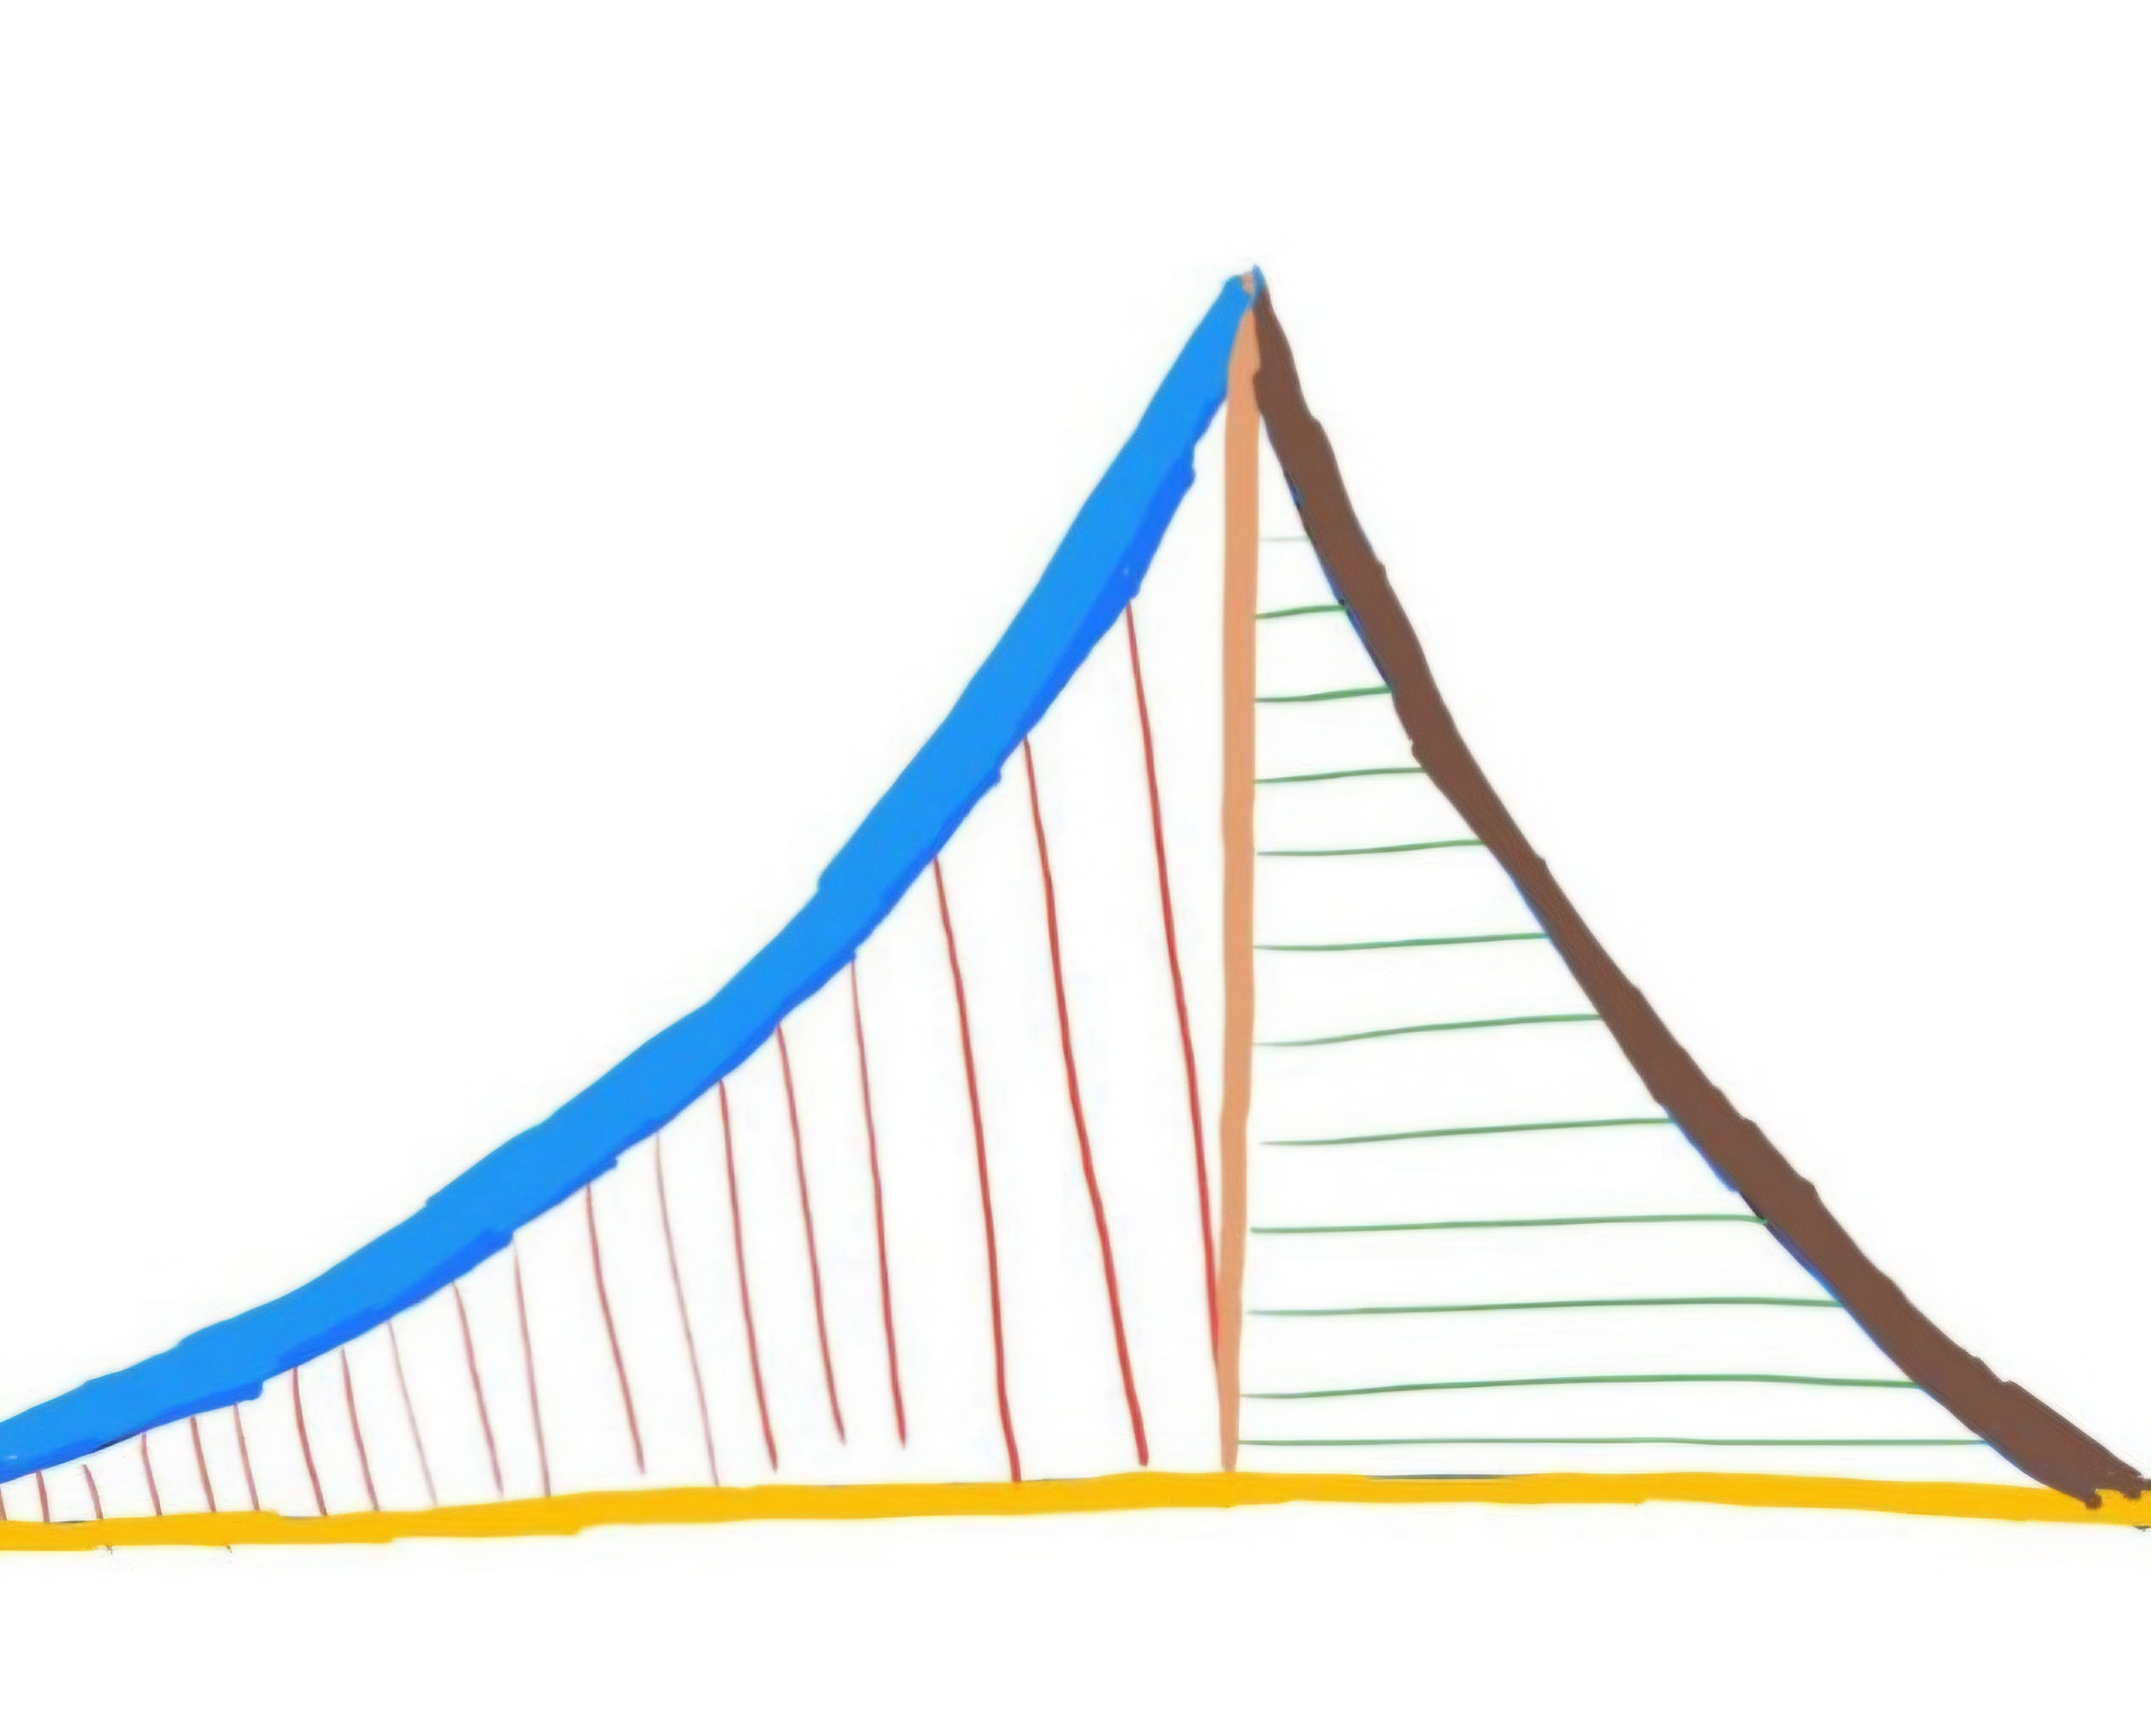
\includegraphics[width=0.2\columnwidth]{figs/logo.jpg}
\\
		{\huge	G. V. V. Sharma}\\Associate Professor,\\Department of Electrical Engineering, \\ IIT Hyderabad
	\end{center}
	%\end{flushleft}
%\IEEEpubid{\makebox[\columnwidth]{978-1-7281-5966-1/20/\$31.00 ©2020 IEEE \hfill} \hspace{\columnsep}\makebox[\columnwidth]{ }}
}
\maketitle

\newpage
\section*{About this Book}

This book introduces trigonometry through high school geometry. This approach relies more on trigonometric equations than cumbersome constructions which are usually non intuitive.
 All problems in the book are from NCERT mathematics textbooks from Class 9-12.  Exercises are from CBSE, JEE and Olympiad exam papers.   

The content is sufficient for all practical applications of trigonometry.
There is no copyright, so readers are free to print and share.  

This book is dedicated to my Hindi teacher in school, Shri Mandavi.
\begin{flushright}
\today
\end{flushright}
Github: https://github.com/gadepall/matgeo
		\\
License: https://creativecommons.org/licenses/by-sa/3.0/
\\
and
\\
https://www.gnu.org/licenses/fdl-1.3.en.html

\newpage


\tableofcontents

\newpage
%\twocolumn
\onecolumn


%\renewcommand{\theequation}{\theenumi}
\numberwithin{equation}{enumi}
%\numberwithin{figure}{enumi}
\numberwithin{figure}{subsection}
%\renewcommand{\thefigure}{\theenumi}
\renewcommand{\thetable}{\theenumi}

\section{Geometry}
%\subsection{Formulae}
%
\subsection{Right Angled Triangle}
\begin{enumerate}[label=\thesubsection.\arabic*.,ref=\thesubsection.\theenumi]
%
	\item 
A right angled triangle looks like Fig. \ref{fig:tri_right_angle}.
\begin{figure}[!ht]
\centering
\resizebox{0.6\columnwidth}{!}{%Code by GVV Sharma
%December 6, 2019
%released under GNU GPL
%Drawing a right angled triangle

\begin{tikzpicture}[scale=2]

%Triangle sides
\def\a{4}
\def\c{3}

%Marking coordiantes
\coordinate [label=above:$A$] (A) at (0,\c);
\coordinate [label=left:$B$] (B) at (0,0);
\coordinate [label=right:$C$] (C) at (\a,0);

%Drawing triangle ABC
\draw (A) -- node[left] {$\textrm{c}$} (B) -- node[below] {$\textrm{a}$} (C) -- node[above,,xshift=2mm] {$\textrm{b}$} (A);

%Drawing and marking angles
\tkzMarkAngle[fill=orange!40,size=0.5cm,mark=](A,C,B)
\tkzMarkRightAngle[fill=blue!20,size=.3](A,B,C)
\tkzLabelAngle[pos=0.65](A,C,B){$\theta$}
\end{tikzpicture}
}
\caption{Right Angled Triangle}
\label{fig:tri_right_angle}	
\end{figure}
with angles $\angle A,\angle B$ and $\angle C$ and sides $a, b$ and $c$.  The unique feature of this triangle is $\angle B$ which is defined to be $90\degree$.
\item
	For simplicity, let the greek letter $\theta = \angle C$.  We have the following definitions.
\begin{equation}
\label{eq:tri_trig_defs}
\begin{matrix}
	\sin \theta = \frac{c}{b} & 	\cos \theta = \frac{a}{b} \\[1ex]
	\tan \theta = \frac{c}{a} & \cot \theta = \frac{1}{\tan \theta} \\[1ex]
	\csc \theta = \frac{1}{\sin \theta} & \sec \theta = \frac{1}{\cos \theta}
	\end{matrix}
\end{equation}
\item  
	\begin{equation}
	\cos \theta = \sin \brak{90\degree - \theta}
	\label{eq:tri_baudh_comp}	
	\end{equation}
\item
In  \figref{fig:tri_baudh}, 
show that 
%
\begin{equation}
\label{ch1_budh_basic}
b = a \cos \theta + c \sin \theta
\end{equation}
%
\begin{figure}[!ht]
	\begin{center}
		\resizebox{0.6\columnwidth}{!}{%Code by GVV Sharma
%December 7, 2019
%released under GNU GPL
%Proof of Baudhyana Theorem

\begin{tikzpicture}
[scale=2,>=stealth,point/.style={draw,circle,fill = black,inner sep=0.5pt},]

%Triangle sides
\def\a{4}
\def\c{3}
\def\b{sqrt(\a^2+\c^2)}

%Trigonometric ratios
\def\ct{\a/\b}
\def\st{\c/\b}

%perp distance
\def\r{\a*\st}

%Section Ratio
\def\k{1.2}


%Labeling points
\node (A) at (0,\c)[point,label=above right:$A$] {};
\node (B) at (0, 0)[point,label=below left:$B$] {};
\node (C) at (\a, 0)[point,label=below right:$C$] {};

%Foot of perpendicular

\node (D) at ($({\r*\st}, {\r*\ct})$)[point,label=above right:$D$] {};


%Drawing triangle ABC
\draw (A) -- node[left] {$\textrm{c}$} (B) -- node[below] {$\textrm{a}$} (C) -- node[above,xshift=2mm] {$\textrm{b}$} (A);

%Joining BD
\draw (B)--(D);

%Drawing and marking angles
\tkzMarkAngle[fill=orange!40,size=0.5cm,mark=](A,C,B)
\tkzMarkAngle[fill=orange!40,size=0.4cm,mark=](D,B,A)
\tkzMarkAngle[fill=green!40,size=0.5cm,mark=](B,A,C)
\tkzMarkAngle[fill=green!40,size=0.5cm,mark=](C,B,D)
\tkzMarkRightAngle[fill=blue!20,size=.2](A,B,C)
\tkzMarkRightAngle[fill=blue!20,size=.2](B,D,A)
\tkzLabelAngle[pos=0.65](A,C,B){$\theta$}
\tkzLabelAngle[pos=0.65](A,B,D){$\theta$}
\tkzLabelAngle[pos=1](B,A,C){\rotatebox{-45}{$\alpha = 90\degree -\theta$}}
\tkzLabelAngle[pos=0.65](C,B,D){$\alpha$}

\end{tikzpicture}
}
	\end{center}
	\caption{Baudhayana Theorem}
	\label{fig:tri_baudh}	
\end{figure}
\solution We observe that
%
\begin{align}
CD &= a \cos \theta \\
AD &= c \cos\alpha = c \sin \theta \quad \brak{\text{From} \quad 
	\eqref{eq:tri_baudh_comp}	
	%\eqref{eq:tri_90-ang}
}
\end{align}
%
Thus,
\begin{equation}
CD + AD = b = a \cos \theta + c \sin \theta
\end{equation}
\item
From \eqref{ch1_budh_basic}, show that
%
\begin{equation}
%
\label{eq:tri_sin_cos_id}
\sin ^2 \theta + \cos ^2 \theta = 1
\end{equation}
%
\solution Dividing both sides of \eqref{ch1_budh_basic} by $b$, 
\begin{align}
1 &= \frac{a}{b}\cos\theta + \frac{c}{b}\sin\theta\\
\Rightarrow &\sin ^2 \theta + \cos ^2 \theta = 1 \quad \brak{\text{from} \quad \eqref{eq:tri_trig_defs}}
\end{align}
%
\item 
From \eqref{eq:tri_sin_cos_id}
\begin{align}
\label{eq:tri_sin_cos_minmax}
	\abs{\sin \theta} \le 1,\
	\abs{\cos \theta} \le 1
\end{align}
\item
	Using \eqref{ch1_budh_basic}, show that
	\begin{equation}
	\label{eq:tri_baudh}
	b^2 = a^2 + c^2
	\end{equation}
	\eqref{eq:tri_baudh} is known as the Baudhayana theorem.  It is also known as the Pythagoras theorem.
\\
\solution From \eqref{ch1_budh_basic},
\begin{align}
b &= a\frac{a}{b} + c \frac{c}{b} \quad \brak{\text{from} \quad \eqref{eq:tri_trig_defs}}\\
\implies b^2 &= a^2 + c^2
\end{align}
%
\item In a right angled triangle, the hypotenuse is the longest side.
\label{them:hyp_largest}
\\
\solution From 
	\eqref{eq:tri_baudh},
\begin{align}
	a \le b,\ c \le b.
\end{align}
\item $ABC$ is an isosceles triangle in which altitudes $BE$ and $CF$ are drawn to equal sides $AC$ and $AB$ respectively . Show that these altitudes are equal.
%
	\\
	\solution In $\triangle$s $BFC$ and $BEC$,
\begin{align}
	\label{eq:tri_isoc-alt}
	BF &= a \sin C,\
	CE = a \sin B 
	\\
	\implies BF &= CE, \because B = C.
\end{align}
\begin{figure}[H]
	\centering
		\resizebox{0.6\columnwidth}{!}{%Code by GVV Sharma
%July 8, 2023
%released under GNU GPL
%Drawing the triangle and angle bisectors


\begin{tikzpicture}
[scale=2,>=stealth,point/.style={draw,circle,fill=black,inner sep=0.5pt}]

% Coordinates of the triangle vertices
\def\a{5}
\def\b{4}
\def\c{4}

% Coordinates of A
\def\p{2.25}
\def\q{{sqrt(\c^2-\p^2)}}

% Labeling points
\node (A) at (\p,\q)[point,label=above right:$A$] {};
\node (B) at (0,0)[point,label=below left:$B$] {};
\node (C) at (\a,0)[point,label=below right:$C$] {};

%\draw (A) -- (B) -- (C) -- (A);
%Drawing triangle ABC
\draw (A) -- node[left] {$\textrm{c}$} (B) -- node[below] {$\textrm{a}$} (C) -- node[above,,xshift=2mm] {$\textrm{b}$} (A);

% Calculating altitudes
\coordinate (F) at ($ (B)!(C)!(A) $); % Foot of altitude from B to AC
\coordinate (E) at ($ (C)!(B)!(A) $); % Foot of altitude from C to AB

% Drawing the altitudes
\draw[dotted] (B) -- (E);
\draw[dotted] (C) -- (F);

% Labeling foot of the altitudes
\node (F) at (F)[point,label=left:$F$] {};
\node (E) at (E)[point,label=right:$E$] {};
\tkzMarkRightAngle[fill=blue!20,size=.2](B,E,A)
\tkzMarkRightAngle[fill=blue!20,size=.2](C,F,B)
\tkzFillAngle[fill=red!20,size=.3](C,B,A)
\tkzFillAngle[fill=red!20,size=.3](A,C,B)


\end{tikzpicture}


}
	\caption{$B = C$}
	\label{fig:tri_isoc-alt}
\end{figure}
\item $ABC$ is a triangle in which altitudes $BE$ and $CF$ to sides $AC$ and $AB$ are equal. Show that
%
$AB = AC$.
%
\\
\solution
	In \eqref{eq:tri_isoc-alt},
\begin{align}
	BE &= CF \implies 
	 a \sin C
	= a \sin B 
	\\
	\text{or, } B &= C
\end{align}
\end{enumerate}
\subsection{Sine and Cosine Formula}
\begin{enumerate}[label=\thesubsection.\arabic*.,ref=\thesubsection.\theenumi]
\item
\label{prob:tri_area_sin}
	Show that the area of $\Delta ABC$ in Fig. 	\ref{fig:tri_sss}	is $\frac{1}{2}ab \sin C$.
\begin{figure}[!ht]
	\begin{center}
			\resizebox{0.6\columnwidth}{!}{%Code by GVV Sharma
%December 7, 2019
%released under GNU GPL
%Drawing a triangle given 3 sides

\begin{tikzpicture}
[scale=2,>=stealth,point/.style={draw,circle,fill = black,inner sep=0.5pt},]

%Triangle sides
\def\a{6}
\def\b{5}
\def\c{4}
 
%Coordinates of A
%\def\p{{\a^2+\c^2-\b^2}/{(2*\a)}}
\def\p{2.25}
\def\q{{sqrt(\c^2-\p^2)}}

%Labeling points
\node (A) at (\p,\q)[point,label=above right:$A$] {};
\node (B) at (0, 0)[point,label=below left:$B$] {};
\node (C) at (\a, 0)[point,label=below right:$C$] {};

%Foot of perpendicular

\node (D) at (\p,0)[point,label=above right:$D$] {};

%Drawing triangle ABC
\draw (A) -- node[left] {$\textrm{c}$} (B) -- node[below] {$\textrm{a}$} (C) -- node[above,xshift=2mm] {$\textrm{b}$} (A);

%Drawing altitude AD
\draw (A) -- node[left] {$\textrm{h}$}(D);

%Drawing and marking angles
%\tkzMarkAngle[fill=orange!40,size=0.5cm,mark=](A,C,B)
%\tkzMarkAngle[fill=orange!40,size=0.4cm,mark=](D,B,A)
%\tkzMarkAngle[fill=green!40,size=0.5cm,mark=](B,A,C)
%\tkzMarkAngle[fill=green!40,size=0.5cm,mark=](C,B,D)
\tkzMarkRightAngle[fill=blue!20,size=.2](A,D,B)
%\tkzMarkRightAngle[fill=blue!20,size=.2](B,D,A)
%\tkzLabelAngle[pos=0.65](A,C,B){$\theta$}
%\tkzLabelAngle[pos=0.65](A,B,D){$\theta$}
%\tkzLabelAngle[pos=1](B,A,C){\rotatebox{-45}{$\alpha = 90\degree -\theta$}}
%\tkzLabelAngle[pos=0.65](C,B,D){$\alpha$}

\end{tikzpicture}
}
	\end{center}
	\caption{Area of a Triangle}
	\label{fig:tri_sss}	
\end{figure}

\solution We have
%
\begin{equation}
ar\brak{\Delta ABC} = \frac{1}{2}ah = \frac{1}{2}ab\sin C \quad \brak{\because \quad h = b \sin C}.
\label{eq:tri_area_sin}
\end{equation}

\item
	Show that 
	\begin{equation}
	\frac{\sin A}{a} = \frac{\sin B}{b} = \frac{\sin C}{c}
	\end{equation}

\solution 
\figref{fig:tri_sss} can be suitably modified to obtain 
\begin{align}
ar\brak{\Delta ABC} = 
\frac{1}{2}ab\sin C = \frac{1}{2}bc\sin A = \frac{1}{2}ca\sin B
	\label{tri:area-sin}
\end{align}
Dividing the above by $abc$, we obtain
	\begin{equation}
\label{eq:tri_sin_form}
	\frac{\sin A}{a} = \frac{\sin B}{b} = \frac{\sin C}{c}
	\end{equation}
This is known as the sine formula.	
%
\item 
	In \figref{fig:tri_isoc}, $AB = AC$.  Show that 
\begin{align}
	\angle B
	= \angle C 
\end{align}
\begin{figure}[H]
	\centering
		\resizebox{0.6\columnwidth}{!}{%Code by GVV Sharma
%July 8, 2023
%released under GNU GPL
%Drawing the triangle and angle bisectors


\begin{tikzpicture}
[scale=2,>=stealth,point/.style={draw,circle,fill=black,inner sep=0.5pt}]

% Coordinates of the triangle vertices
\def\a{5}
\def\b{4}
\def\c{4}

% Coordinates of A
\def\p{2.25}
\def\q{{sqrt(\c^2-\p^2)}}

% Labeling points
\node (A) at (\p,\q)[point,label=above right:$A$] {};
\node (B) at (0,0)[point,label=below left:$B$] {};
\node (C) at (\a,0)[point,label=below right:$C$] {};

% Drawing triangle ABC
\draw (A) -- (B) -- (C) -- (A);

% Calculating the coordinates of E using the angle bisector theorem
%\coordinate (E) at ($(A)!\b/(\b+\c)!(C)$);

% Drawing the angle bisector BE
%\draw[dashed] (B) -- (E);

% Labeling point E
%\node (E) at (E)[point,label=below right:$E$] {};

% Calculating the coordinates of F using the angle bisector theorem
%\coordinate (F) at ($(A)!\c/(\b+\c)!(B)$);

% Drawing the angle bisector CF
%\draw[dashed] (C) -- (F);

% Labeling point F
%\node (F) at (F)[point,label=below left:$F$] {};

% Calculating the intersection point O of BE and CF
%\coordinate (O) at (intersection of B--E and C--F);

% Drawing the intersection point O
%\node (O) at (O)[point,label=above:$O$] {};


\end{tikzpicture}


}
	\caption{}
	\label{fig:tri_isoc}
\end{figure}
\solution Using the sine formula, 
\begin{align}
	\frac{AB}{\sin C}
	&=\frac{AC}{\sin B}
	\\
	\implies \sin B &= \sin C
	\text{ or, } \angle B = \angle C.
\end{align}
%\end{enumerate}
\item
In Fig. \ref{fig:tri_cosine_formula}, show that
%
\begin{equation}
\label{eq:tri_cos_mat}
\begin{pmatrix}
0 & c & b \\
c & 0 & a \\
b & a & 0
\end{pmatrix}
\begin{pmatrix}
\cos A \\
\cos B \\
\cos C
\end{pmatrix}
= 
\begin{pmatrix}
a\\
b\\
c
\end{pmatrix}
\end{equation}
%
%
\begin{figure}[!ht]
	\begin{center}
		
		%\includegraphics[width=0.6\columnwidth]{figs/ch2_triang_ar}
		%\vspace*{-10cm}
		\resizebox{0.6\columnwidth}{!}{%Code by GVV Sharma
%December 7, 2019
%released under GNU GPL
%Drawing a triangle given 3 sides

\begin{tikzpicture}
[scale=2,>=stealth,point/.style={draw,circle,fill = black,inner sep=0.5pt},]

%Triangle sides
\def\a{6}
\def\b{5}
\def\c{4}
 
%Coordinates of A
%\def\p{{\a^2+\c^2-\b^2}/{(2*\a)}}
\def\p{2.25}
\def\q{{sqrt(\c^2-\p^2)}}

%Labeling points
\node (A) at (\p,\q)[point,label=above right:$A$] {};
\node (B) at (0, 0)[point,label=below left:$B$] {};
\node (C) at (\a, 0)[point,label=below right:$C$] {};

%Foot of perpendicular

\node (D) at (\p,0)[point,label=above right:$D$] {};

%Drawing triangle ABC
\draw (A) -- node[left] {$\textrm{c}$} (B) -- node[below] {$\textrm{a}$} (C) -- node[above,xshift=2mm] {$\textrm{b}$} (A);

%Drawing altitude AD
\draw (A) -- node[left] {$\textrm{h}$}(D);

\tkzMarkRightAngle[fill=blue!20,size=.2](A,D,B)

\node [below] at ($(B)!0.5!(D)$) {$x$};
\node [below] at ($(C)!0.5!(D)$) {$y$};

\end{tikzpicture}
}
	\end{center}
	\caption{The cosine formula}
	\label{fig:tri_cosine_formula}	
\end{figure}
\solution From Fig. \ref{fig:tri_cosine_formula}, 
%
\begin{align}
	a = x + y &= b \cos C + c \cos B = \myvec{  \cos C & \cos B } \myvec{ b \\ c }
	\\
&=\myvec{0 & b & c } \myvec{ \cos A \\ \cos C \\ \cos B } 
\end{align}
%
Similarly,
%
\begin{align}
b &= c \cos A + a \cos C 
=\myvec{c & 0 & a } \myvec{ \cos A \\ \cos C \\ \cos B } 
	\\
c &= b \cos A + a \cos B
=\myvec{b & a & 0 } \myvec{ \cos A \\ \cos C \\ \cos B } 
\end{align}
%
The above equations can be expressed in matrix form as
\eqref{eq:tri_cos_mat}.

\item Show that 
\begin{equation}
\label{eq:tri_cos_form}
\cos A = \frac{b^2+c^2-a^2}{2bc}
\end{equation}
%
\solution 
Using the properties of determinants,
%
\begin{align}
\cos A = \frac{
\begin{vmatrix}
a & c & b \\
b & 0 & a \\
c & a & 0
\end{vmatrix}
	}
	{
\begin{vmatrix}
0 & c & b \\
c & 0 & a \\
b & a & 0
\end{vmatrix}
	}
	=\frac{ab^2 + ac^2 - a^3}{abc + abc} 
= \frac{b^2 + c^2 - a^2}{2abc}
\end{align}
%
\item Find Hero's formula for the area of a triangle.
\\
\solution 
From \eqref{prob:tri_area_sin}, the area of $\triangle ABC$ is 
\begin{align}
\label{eq:tri_geo_area_sin_form}
 \frac{1}{2}ab\sin C
%\\
&=\frac{1}{2}ab\sqrt{1-\cos^2C} 
\quad \brak{\text{from } \eqref{eq:tri_sin_cos_id}
%\eqref{eq:tri_geo_baudh}
}
\\
&=\frac{1}{2}ab\sqrt{1-\brak{\frac{a^2+b^2-c^2}{2ab}}^2} \brak{\text{from } \eqref{eq:tri_cos_form}
}
\\
&=\frac{1}{4}\sqrt{\brak{2ab}^2-\brak{a^2+b^2-c^2}}
\\
&=\frac{1}{4}\sqrt{\brak{2ab+a^2+b^2-c^2}\brak{2ab-a^2-b^2+c^2}}
\\
&= \frac{1}{4}\sqrt{\cbrak{\brak{a+b}^2-c^2}\cbrak{c^2-\brak{a-b}^2}}
\\
&= \frac{1}{4}\sqrt{\brak{a+b+c}\brak{a+b-c}\brak{a+c-b}\brak{b+c-a}}
\label{eq:tri_ex_hero_temp}
\end{align}
Substituting 
%
\begin{align}
s=\frac{a+b+c}{2}
\end{align}
%
in \eqref{eq:tri_ex_hero_temp}, the area of $\triangle ABC$ is 
%
\begin{align}
\label{eq:tri_area_hero}
\sqrt{s\brak{s-a}\brak{s-b}\brak{s-c}}
\end{align}
%
This is known as Hero's formula.
\item Show that 
%
\begin{align}
\label{eq:trig_id_sin_inc}
\alpha > \beta \implies \sin \alpha > \sin \beta
\end{align}
%

\begin{figure}[!ht]
	\begin{center}
		
		%\includegraphics[width=\columnwidth]{figs/fig:tri_sin_inc}
		%\vspace*{-10cm}
		\resizebox{0.6\columnwidth}{!}{\begin{tikzpicture}
[scale =3,>=stealth,point/.style = {draw, circle, fill = black, inner sep = 1pt},]

\node (A) at (0,3)[point,label=above :$A$] {};
\node (B) at (3,0)[point,label=below :$B$] {};
\node (C) at (0,0)[point,label=below :$C$] {};
\node (D) at (0,1.5)[point,label=left :$D$] {};
\draw (A)--(B);
\draw (C)--(B);
\draw (A)--(C);
\draw (B)--(D);
\tkzMarkAngle[size=.4](A,B,D);
\tkzMarkAngle[size=.3](D,B,C);
\tkzMarkRightAngle[size=.15](A,C,B);

\node [above] at (1.6,1.5){$c$};
\node [below] at (1.6,0){$a$};
\node [below] at (1.6,1){$l$};
\node [above] at (-0.2,1.5){$b$};
\node [above] at (2.5,0){$\theta_2$};
\node [above] at (2.5,0.3){$\theta_1$};
\end{tikzpicture}}
	\end{center}
	\caption{}
	%\caption{$\sin \brak{\theta_1+\theta_2} = \sin\theta_1\cos\theta_2 + \cos\theta_1\sin\theta_2$}
	\label{fig:tri_sin_inc}	
\end{figure}
\solution In Fig. \ref{fig:tri_sin_inc}, 	
%
\begin{align}
ar\brak{\triangle ABD} &< ar \brak{\triangle ABC}
\\
\implies \frac{1}{2}lc \sin \theta_1 &<  \frac{1}{2}ac \sin \brak{\theta_1 + \theta_2 }
\\
\implies \frac{l}{a} &< \frac{\sin \brak{\theta_1 + \theta_2 }}{\sin \theta_1}
\\
\text{or, } 1 < \frac{l}{a} &< \frac{\sin \brak{\theta_1 + \theta_2 }}{\sin \theta_1}
\end{align}
%
from Theorem \ref{them:hyp_largest}, yielding 
\begin{align}
\implies \frac{\sin \brak{\theta_1 + \theta_2 }}{\sin \theta_1} > 1.
\end{align}

This proves \eqref{eq:trig_id_sin_inc}.
\end{enumerate}
%
\subsection{Trigonometric Identities}
\begin{enumerate}[label=\thesubsection.\arabic*.,ref=\thesubsection.\theenumi]
\item
	Using 
	\figref{fig:tri_sin_inc},
%Fig. \ref{trig_id_sin_theta}, 
show that 
	%
\begin{equation}
\label{trig_id_sin_theta_eq}
\sin  \theta_1 = \sin \brak{\theta_1 + \theta_2}\cos \theta_2 - \cos\brak{\theta_1+\theta_2}\sin\theta_2
\end{equation}	
	%
\iffalse
\begin{figure}[!ht]
	\begin{center}
		
		%\includegraphics[width=0.6\columnwidth]{figs/trig_id_sin_theta}
		%\vspace*{-10cm}
		\resizebox{0.6\columnwidth}{!}{\begin{tikzpicture}
[scale =3,>=stealth,point/.style = {draw, circle, fill = black, inner sep = 1pt},]

\node (A) at (0,3)[point,label=above :$A$] {};
\node (B) at (3,0)[point,label=below :$B$] {};
\node (C) at (0,0)[point,label=below :$C$] {};
\node (D) at (0,1.5)[point,label=left :$D$] {};
\draw (A)--(B);
\draw (C)--(B);
\draw (A)--(C);
\draw (B)--(D);
\tkzMarkAngle[size=.4](A,B,D);
\tkzMarkAngle[size=.3](D,B,C);
\tkzMarkRightAngle[size=.15](A,C,B);

\node [above] at (1.6,1.5){$c$};
\node [below] at (1.6,0){$a$};
\node [below] at (1.6,1){$l$};
\node [above] at (-0.2,1.5){$b$};
\node [above] at (2.5,0){$\theta_2$};
\node [above] at (2.5,0.3){$\theta_1$};
\end{tikzpicture}}
	\end{center}
	\caption{$\sin \brak{\theta_1+\theta_2} = \sin\theta_1\cos\theta_2 + \cos\theta_1\sin\theta_2$}
	\label{trig_id_sin_theta}	
\end{figure}
\fi
%

\solution The following equations can be obtained from the figure using the forumula for the area of a triangle
%
\begin{align}
ar \brak{\Delta ABC} &= \frac{1}{2}ac \sin\brak{\theta_1 + \theta_2} \\
&= ar \brak{\Delta BDC} + ar \brak{\Delta ADB} \\
&= \frac{1}{2}cl \sin{\theta_1} + \frac{1}{2}al \sin{\theta_2} \\ 
&= \frac{1}{2}ac \sin{\theta_1} \sec \theta_2 + \frac{1}{2}a^2 \tan{\theta_2} 
\end{align}
$\brak{\because
	l = a \sec \theta_2}$.  From the above,
\begin{align}
\sin\brak{\theta_1 + \theta_2} &=  \sin{\theta_1} \sec \theta_2 + \frac{a}{c} \tan{\theta_2} \\
	&=  \sin{\theta_1} \sec \theta_2 
+ \cos\brak{\theta_1 + \theta_2} \tan{\theta_2} 
\end{align}
Multiplying both sides by $\cos \theta_2$,
\begin{align}
\sin\brak{\theta_1 + \theta_2}\cos{\theta_2} =  \sin{\theta_1}  
+ \cos\brak{\theta_1 + \theta_2} \sin\theta_2  
\end{align}
%
resulting in
\eqref{trig_id_sin_theta_eq}.
\item
	Prove the following identities 
	%
	\begin{enumerate}
\item 
\begin{equation}
		\label{trig_id_sin_diff}
\sin\brak{\alpha - \beta} = \sin \alpha \cos \beta - \cos \alpha \sin \beta.
\end{equation}
\item 
\begin{equation}
\cos\brak{\alpha + \beta} = \cos \alpha \cos \beta - \sin \alpha \sin \beta.
		\label{trig_id_cos_diff}
\end{equation}

	\end{enumerate}
	%

\solution In \eqref{trig_id_sin_theta_eq}, let
%
\begin{equation}
\begin{split}
\theta_1 + \theta_2 &= \alpha \\
\theta_2 &=  \beta
\end{split}
\end{equation}
%
This gives \eqref{trig_id_sin_diff}.  In \eqref{trig_id_sin_diff}, replace $\alpha$ by 
%
$90{\degree} - \alpha$.  This results in
%
\begin{align}
\sin\brak{90{\degree} - \alpha - \beta}
	&=
\sin \brak{90{\degree} -\alpha} \cos \beta - \cos \brak{90{\degree} -\alpha} \sin \beta \\
	\implies \cos\brak{\alpha + \beta} &= \cos \alpha \cos \beta - \sin \alpha \sin \beta
\end{align}
% 
\item
	Using \eqref{trig_id_sin_theta_eq} and \eqref{trig_id_cos_diff}, show that
\begin{align}
\label{trig_id_sin_sum}
\sin\brak{\theta_1 + \theta_2} &= \sin\theta_1  \cos\theta_2 + \cos\theta_1\sin\theta_2
\\
\cos\brak{\theta_1 - \theta_2} &= \cos\theta_1  \cos\theta_2  \sin\theta_1\sin\theta_2
\label{trig_id_cos_sum}
\end{align}

%
\solution From \eqref{trig_id_sin_theta_eq},
%
\begin{align}
 \sin \brak{\theta_1 + \theta_2}\cos \theta_2 =\sin  \theta_1 +\cos\brak{\theta_1+\theta_2}\sin\theta_2 
\end{align}
%
Using \eqref{trig_id_cos_diff} in the above,
%
\begin{align}
\sin \brak{\theta_1 + \theta_2}\cos \theta_2 
=\sin  \theta_1 +\brak{\cos \theta_1\cos\theta_2 
	- \sin \theta_1\sin\theta_2}\sin\theta_2 
\end{align}
%
which can be expressed as
%
\begin{align}
\sin \brak{\theta_1 + \theta_2}\cos \theta_2 
=\sin  \theta_1 
+\cos \theta_1\cos\theta_2 \sin\theta_2 
		- \sin \theta_1\sin^2\theta_2
\end{align}
%
Since
%
\begin{equation}
\sin^2\theta_2 = 1- \cos^2\theta_2, 
\end{equation}
%
we obtain
%
\begin{align}
\sin \brak{\theta_1 + \theta_2}\cos \theta_2 
=\cos \theta_1\cos\theta_2 \sin\theta_2 
+ \sin \theta_1\cos^2\theta_2
\end{align}
%
resulting in
%
\begin{equation}
\sin \brak{\theta_1 + \theta_2}
=\cos \theta_1 \sin\theta_2 
+ \sin \theta_1\cos\theta_2
\end{equation}
%
after factoring out $\cos \theta_2$.  Using a similar approach, \eqref{trig_id_cos_sum} can also be proved.
\item Show that 
\begin{align}
\label{eq:trig_id_sum_diff1}
\sin \theta_1 + \sin \theta_2 &= 2\sin\brak{\frac{\theta_1+\theta_2}{2}}\cos\brak{\frac{\theta_1-\theta_2}{2}}
\\
\label{eq:trig_id_sum_diff2}
\cos \theta_1 + \cos \theta_2 &= 2\cos\brak{\frac{\theta_1+\theta_2}{2}}\cos\brak{\frac{\theta_1-\theta_2}{2}}
\\
\label{eq:trig_id_sum_diff3}
\sin \theta_1 - \sin \theta_2 &= 2\sin\brak{\frac{\theta_1-\theta_2}{2}}\cos\brak{\frac{\theta_1+\theta_2}{2}}
\\
\label{eq:trig_id_sum_diff4}
\cos \theta_1 - \cos \theta_2 &= 2\sin\brak{\frac{\theta_1+\theta_2}{2}}\cos\brak{\frac{\theta_2-\theta_1}{2}}
\end{align}
%
\\
\solution Let 
%
\begin{align}
\label{eq:trig_id_ang_sum_diff}
\begin{split}
\theta_1 = \alpha + \beta
\\
\theta_2 = \alpha - \beta
\end{split}
\end{align}
%
From \eqref{trig_id_sin_sum},
%
\begin{align}
\sin \theta_1 + \sin \theta_2  &= \sin \brak{\alpha + \beta} + \sin \brak{\alpha - \beta}
\\
&= \sin \alpha \cos \beta + \cos \alpha \sin \beta 
+\sin \alpha \cos \beta - \cos \alpha \sin \beta
\\
&= 2 \sin \alpha \cos \beta
\end{align}
%
resulting in \eqref{eq:trig_id_sum_diff1}
%
\begin{align}
\because \alpha = \frac{\theta_1 +\theta_2}{2}
,\
\beta = \frac{\theta_1 -\theta_2}{2}
\end{align}
from \eqref{eq:trig_id_ang_sum_diff}.  Other identities may be proved similarly.
%
\item Show that 
  \begin{align}
\label{eq:trig-id-2A-sin}
	  \sin 2 \theta &= 2 \sin \theta \cos \theta
	  \\
	  \cos 2 \theta &= 1 - 2 \sin^2 \theta 
	  =  2 \cos^2 \theta -1
	  \\
	  &= \cos^2 \theta -\sin^2 \theta 
\label{eq:trig-id-2A-cos}
  \end{align}
\end{enumerate}
%
\subsection{Incircle}
\begin{enumerate}[label=\thesubsection.\arabic*.,ref=\thesubsection.\theenumi]
\item  In  
	\figref{fig:tri_icentre}, the bisectors of $\angle B$ and $\angle C$	 meet at $\vec{I}$.
Show that $IA$ bisects $\angle A$.
\begin{figure}[!ht]
	\begin{center}
		
		\resizebox{0.6\columnwidth}{!}{%Code by GVV Sharma
%July 4, 2023
%released under GNU GPL
%Angle bisectors are concurrent

\begin{tikzpicture}
[scale=2,>=stealth,point/.style={draw,circle,fill = black,inner sep=0.5pt},]

%Triangle sides
\def\a{5}
\def\b{6}
\def\c{4}
 
%Coordinates of A
%\def\p{{\a^2+\c^2-\b^2}/{(2*\a)}}
\def\p{0.5}
\def\q{{sqrt(\c^2-\p^2)}}

%Labeling points
\node (A) at (\p,\q)[point,label=above right:$A$] {};
\node (B) at (0, 0)[point,label=below left:$B$] {};
\node (C) at (\a, 0)[point,label=below right:$C$] {};

%Circumcentre

\node (I) at (1.5,1.32287566)[point,label=right:$I$] {};
\node (D) at (1.5,0) {};
\node (E) at (2.375,2.3150324) {};
\node (F) at (0.1875,1.48823511) {};

%Drawing triangle ABC
%\draw (A) -- node[left] {$\textrm{c}$} (B) -- node[below] {$\textrm{a}$} (C) -- node[above,yshift=2mm] {$\textrm{b}$} (A);
\draw (A) --   (B) --   (C) --   (A);
%Drawing OA, OB, OC
\draw (I) -- node[right] {$l_1$}(A);
\draw (I) --  node[left,yshift=1mm] {$l_2$}(B);
\draw (I) --  node[right,yshift=2mm] {$l_3$}(C);

\iffalse
%Drawing OD, OE, OF
\draw (I) -- node[right] {$\textrm{r}$} (D);
\draw (I) -- node[below] {$\textrm{r}$} (E);
\draw (I) -- node[below] {$\textrm{r}$} (F);
\fi

\tkzMarkAngle[fill=green!60,size=.3](I,B,F)
\tkzMarkAngle[fill=green!40,size=.3](D,B,I)
%
%
\tkzMarkAngle[size=.3](F,A,I)
\tkzMarkAngle[size=.4](I,A,E)
\iffalse
\tkzMarkAngle[fill=red!60,size=.3](F,A,I)
\tkzMarkAngle[fill=red!40,size=.3](I,A,E)
\fi


\tkzMarkAngle[fill=orange!60](E,C,I)
\tkzMarkAngle[fill=orange!40](I,C,D)
%
\iffalse
\tkzMarkRightAngle[fill=blue!20,size=.3](A,E,I)
\tkzMarkRightAngle[fill=blue!20,size=.3](A,F,I)
\tkzMarkRightAngle[fill=blue!20,size=.3](I,D,C)

%Labeling x,y,z
\node (x1) at ($(B)!0.5!(D)$)[label=below:$x$] {};
\node (x2) at ($(B)!0.5!(F)$)[label=left:$x$] {};
\node (y1) at ($(C)!0.5!(D)$)[label=below:$y$] {};
\node (y2) at ($(C)!0.5!(E)$)[label=right:$y$] {};
\node (z1) at ($(A)!0.5!(E)$)[label=right:$z$] {};
\node (z2) at ($(A)!0.5!(F)$)[label=left:$z$] {};
\fi

\tkzLabelAngle[pos=0.65](B,A,I){$\theta$}
\tkzLabelAngle[pos=0.85,sloped](I,A,C){$A - \theta$}

\end{tikzpicture}
}
	\end{center}
	\caption{Incentre $I$ of $\triangle ABC$}
	\label{fig:tri_icentre}	
\end{figure}
\\
\solution
Using sine formula
in
\eqref{eq:tri_sin_form}
  \begin{align}
  \frac{l_1}{\sin\frac{C}{2}}
  = 
   \frac{l_3}{\sin \brak{A-\theta}}
  ,\
   \frac{l_3}{\sin\frac{B}{2}}
=\frac{l_2}{\sin\frac{C}{2}}
  ,\
\frac{l_2}{\sin \theta}
	  =
  \frac{l_1}{\sin\frac{B}{2}}
  \end{align}
  Multiplying the above equations, 
  \begin{align}
  \sin \theta &= \sin \brak{A - \theta}
  \\
	  \implies \theta &=A - \theta 
	  \text{ or, } \theta = \frac{A}{2}
  \end{align}
  \item 
	\figref{fig:tri_iradius}, 
	is obtained from 
	\figref{fig:tri_icentre}	
	with
  \begin{align}
	  ID \perp BC, \, 
	  IE \perp AC, \, 
	  IF \perp AB.
  \end{align}
  Show that 
  \begin{align}
	  ID=   
	  IE= 
	  IF=r 
	\label{eq:tri_iradius}	
  \end{align}
		\begin{figure}[!ht]
	\begin{center}
		\resizebox{0.6\columnwidth}{!}{%Code by GVV Sharma
%July 4, 2023
%released under GNU GPL
%Distance for the incentre to the sides is the same

\begin{tikzpicture}
[scale=2,>=stealth,point/.style={draw,circle,fill = black,inner sep=0.5pt},]

%Triangle sides
\def\a{5}
\def\b{6}
\def\c{4}
 
%Coordinates of A
%\def\p{{\a^2+\c^2-\b^2}/{(2*\a)}}
\def\p{0.5}
\def\q{{sqrt(\c^2-\p^2)}}

%Labeling points
\node (A) at (\p,\q)[point,label=above right:$A$] {};
\node (B) at (0, 0)[point,label=below left:$B$] {};
\node (C) at (\a, 0)[point,label=below right:$C$] {};

%Incentre

\node (I) at (1.5,1.32287566)[point,label=right:$I$] {};
\node (D) at (1.5,0)[point,label=below:$D$] {};
\node (E) at (2.375,2.3150324)[point,label=above right:$E$] {};
\node (F) at (0.1875,1.48823511)[point,label=left:$F$] {};

%Drawing triangle ABC
%\draw (A) -- node[left] {$\textrm{c}$} (B) -- node[below] {$\textrm{a}$} (C) -- node[above,yshift=2mm] {$\textrm{b}$} (A);
\draw (A) --   (B) --   (C) --   (A);
%Drawing OA, OB, OC
\draw (I) -- node[right] {$l_1$}(A);
\draw (I) --  node[left,yshift=1mm] {$l_2$}(B);
\draw (I) --  node[right,yshift=2mm] {$l_3$}(C);

%Drawing OD, OE, OF
\draw (I) -- node[right] {$\textrm{r}$} (D);
\draw (I) --  (E);
\draw (I) --  (F);

\tkzMarkAngle[fill=green!60,size=.3](I,B,F)
\tkzMarkAngle[fill=green!40,size=.3](D,B,I)
%
%
\iffalse
\tkzMarkAngle[size=.3](F,A,I)
\tkzMarkAngle[size=.4](I,A,E)
\fi
\tkzMarkAngle[fill=red!60,size=.3](F,A,I)
\tkzMarkAngle[fill=red!40,size=.3](I,A,E)


\tkzMarkAngle[fill=orange!60](E,C,I)
\tkzMarkAngle[fill=orange!40](I,C,D)
%
\tkzMarkRightAngle[fill=blue!20,size=.3](A,E,I)
\tkzMarkRightAngle[fill=blue!20,size=.3](A,F,I)
\tkzMarkRightAngle[fill=blue!20,size=.3](I,D,C)
\iffalse

%Labeling x,y,z
\node (x1) at ($(B)!0.5!(D)$)[label=below:$x$] {};
\node (x2) at ($(B)!0.5!(F)$)[label=left:$x$] {};
\node (y1) at ($(C)!0.5!(D)$)[label=below:$y$] {};
\node (y2) at ($(C)!0.5!(E)$)[label=right:$y$] {};
\node (z1) at ($(A)!0.5!(E)$)[label=right:$z$] {};
\node (z2) at ($(A)!0.5!(F)$)[label=left:$z$] {};

\tkzLabelAngle[pos=0.65](B,A,I){$\theta$}
\tkzLabelAngle[pos=0.85,sloped](I,A,C){$A - \theta$}
\fi

\end{tikzpicture}
}
	\end{center}
	\caption{Inradius $r$ of $\triangle ABC$}
	\label{fig:tri_iradius}	
\end{figure}
		\solution
In $\triangle$s $IDC$ and $IEC$, 
		\begin{align}
ID = IE=  \frac{l_3}{\sin\frac{C}{2}}
		\end{align}
		Similarly, 
in $\triangle$s $IEA$ and $IFA$, 
		\begin{align}
IF = IE=  \frac{l_1}{\sin\frac{A}{2}}
		\end{align}
		yielding 
	\eqref{eq:tri_iradius}	
  \item In
	\figref{fig:tri_iradius}, show that
  \begin{align}
	  BD=BF ,\, 
	  AE=AF ,\, 
	  CD=CE 
  \end{align}
  \solution  From 
\figref{fig:tri_iradius}, in $\triangle$s $IBD$ and $IBF$, 
		\begin{align}
			x = BD = BF = r \cot \frac{B}{2}
		\end{align}
		Similarly, other results can be obtained.
\item The circle with centre $\vec{I}$ and radius $r$ in  
	\figref{fig:tri_icircle}	
is known as the {\em incircle}. 
\begin{figure}[!ht]
	\begin{center}
		\resizebox{0.6\columnwidth}{!}{%Code by GVV Sharma
%December 10, 2019
%released under GNU GPL
%Drawing the incircle

\begin{tikzpicture}
[scale=2,>=stealth,point/.style={draw,circle,fill = black,inner sep=0.5pt},]

%Triangle sides
\def\a{5}
\def\b{6}
\def\c{4}

%Inradius
\def\r{1.3228756555322954}
 
%Coordinates of A
%\def\p{{\a^2+\c^2-\b^2}/{(2*\a)}}
\def\p{0.5}
\def\q{{sqrt(\c^2-\p^2)}}

%Labeling points
\node (A) at (\p,\q)[point,label=above right:$A$] {};
\node (B) at (0, 0)[point,label=below left:$B$] {};
\node (C) at (\a, 0)[point,label=below right:$C$] {};

%Circumcentre

\node (I) at (1.5,1.32287566)[point,label=right:$I$] {};
\node (D) at (1.5,0)[point,label=below:$D$] {};
\node (E) at (2.375,2.3150324)[point,label=above right:$E$] {};
\node (F) at (0.1875,1.48823511)[point,label=left:$F$] {};

%Drawing triangle ABC
\draw (A) -- node[left] {$\textrm{c}$} (B) -- node[below] {$\textrm{a}$} (C) -- node[above,yshift=2mm] {$\textrm{b}$} (A);
%Drawing OA, OB, OC
\draw (I) --  (A);
\draw (I) --  (B);
\draw (I) --  (C);

%Drawing OD, OE, OF
\draw (I) -- node[right] {$\textrm{r}$} (D);
\draw (I) -- node[below] {$\textrm{r}$} (E);
\draw (I) -- node[below] {$\textrm{r}$} (F);

%Drawing Incircle
\draw (I) circle (\r);



\tkzMarkAngle[fill=green!60,size=.3](I,B,F)
\tkzMarkAngle[fill=green!40,size=.3](D,B,I)
%
%
\tkzMarkAngle[fill=red!60,size=.3](F,A,I)
\tkzMarkAngle[fill=red!40,size=.3](I,A,E)


\tkzMarkAngle[fill=orange!60](E,C,I)
\tkzMarkAngle[fill=orange!40](I,C,D)
%
\tkzMarkRightAngle[fill=blue!20,size=.3](A,E,I)
\tkzMarkRightAngle[fill=blue!20,size=.3](A,F,I)
\tkzMarkRightAngle[fill=blue!20,size=.3](I,D,C)

%Labeling x,y,z
\node (x1) at ($(B)!0.5!(D)$)[label=below:$x$] {};
\node (x2) at ($(B)!0.5!(F)$)[label=left:$x$] {};
\node (y1) at ($(C)!0.5!(D)$)[label=below:$y$] {};
\node (y2) at ($(C)!0.5!(E)$)[label=right:$y$] {};
\node (z1) at ($(A)!0.5!(E)$)[label=right:$z$] {};
\node (z2) at ($(A)!0.5!(F)$)[label=left:$z$] {};


\end{tikzpicture}
}
	\end{center}
	\caption{Incircle of $\triangle ABC$}
	\label{fig:tri_icircle}	
\end{figure}
\item The lengths of tangents drawn from an external point to a circle are equal.
\item In an isosceles $\triangle ABC$, with $AB = AC$, $BE$ and $CF$ are the bisectors of $\angle B$ and $\angle C$ respectively.   Show that 
\begin{align}
BE = CF
	\label{eq:tri_isoc_ang_bsect}
\end{align}
\begin{figure}[H]
	\centering
		\resizebox{0.6\columnwidth}{!}{%Code by GVV Sharma
%July 8, 2023
%released under GNU GPL
%Drawing the triangle and angle bisectors


\begin{tikzpicture}
[scale=2,>=stealth,point/.style={draw,circle,fill=black,inner sep=0.5pt}]

% Coordinates of the triangle vertices
\def\a{5}
\def\b{4}
\def\c{4}

% Coordinates of A
\def\p{2.25}
\def\q{{sqrt(\c^2-\p^2)}}

% Labeling points
\node (A) at (\p,\q)[point,label=above right:$A$] {};
\node (B) at (0,0)[point,label=below left:$B$] {};
\node (C) at (\a,0)[point,label=below right:$C$] {};

% Drawing triangle ABC
\draw (A) -- (B) -- (C) -- (A);

% Calculating the coordinates of E using the angle bisector theorem
\coordinate (E) at ($(A)!\b/(\b+\c)!(C)$);

% Drawing the angle bisector BE
\draw[dashed] (B) -- (E);

% Labeling point E
\node (E) at (E)[point,label=below right:$E$] {};

% Calculating the coordinates of F using the angle bisector theorem
\coordinate (F) at ($(A)!\c/(\b+\c)!(B)$);

% Drawing the angle bisector CF
\draw[dashed] (C) -- (F);

% Labeling point F
\node (F) at (F)[point,label=below left:$F$] {};

% Calculating the intersection point O of BE and CF
\coordinate (I) at (intersection of B--E and C--F);

% Drawing the intersection point O
%\node (I) at (I)[point,label=above:$I$] {};


\end{tikzpicture}


}
	\caption{}
	\label{fig:tri_isoc_ang_bsect}
\end{figure}
\solution
%
In $\triangle$ s $BEC$ and $BFC$, using the sine formula, 
\begin{align}
	\label{eq:tri_isoc_ang_bsect-inter}
\begin{split}
	\frac{BE}{\sin C}
	&=\frac{BC}{\sin \brak{\frac{B}{2}+C}}
	\\
	\frac{CF}{\sin B}
	&=\frac{BC}{\sin \brak{\frac{C}{2}+B}}
\end{split}
\end{align}
$\because B = C$, from the above, we obtain
	\eqref{eq:tri_isoc_ang_bsect}.
\item Show that
\begin{align}
\sin 5\theta &= 5\sin \theta - 20\sin^3 \theta \cos^2 \theta + 16\sin^5 \theta \\
\sin 3\theta &= 3\sin \theta - 4\sin^3 \theta
\label{eq:sin3-5}
\end{align}
\item 
	In \figref{fig:tri_isoc_ang_bsect}, if $BE = CF$, show that the triangle is isosceles.
	\\
	\solution
	From \eqref{eq:tri_isoc_ang_bsect-inter},
\begin{align}
	\sin C
\sin \brak{\frac{C}{2}+B}
	&=
\sin \brak{\frac{B}{2}+C}
\sin B
\\
	\implies 2\sin C
\sin \brak{\frac{C}{2}+B}
	&=
2\sin B
\sin \brak{\frac{B}{2}+C}
\\
\cos \brak{B - \frac{C}{2}}
-\cos \brak{B + \frac{3C}{2}}
	&=
\cos \brak{C - \frac{B}{2}}
-\cos \brak{C + \frac{3B}{2}}
\end{align}
using \eqref{eq:trig_id_sum_diff4},
which can be expressed as
\begin{align}
\cos \brak{C - \frac{B}{2}}
-
\cos \brak{B - \frac{C}{2}}
-\cos \brak{C + \frac{3B}{2}}
+
	\cos \brak{B + \frac{3C}{2}}
	=0
\end{align}
which, using \eqref{eq:trig_id_sum_diff4},
yields
\begin{align}
 2\sin \brak{ \frac{B +C}{2}}
	\sin \sbrak{ \frac{3\brak{B -C}}{2}}
	+ 2\sin \sbrak{ 5\frac{\brak{B +C}}{2}}
	\sin \sbrak{ \frac{\brak{B -C}}{2}}
	=0
\label{eq:bisect-conv}
\end{align}
Let
\begin{align}
	\theta = \frac{B -C}{2},\
	\alpha= \frac{B +C}{2}
\end{align}
Substituting the above in 
\eqref{eq:bisect-conv},
\begin{align}
 \sin \alpha \sin 3\theta
	+ \sin 5 \alpha \sin \theta = 0
\label{eq:bisect-conv-at}
\end{align}
Substituting
from \eqref{eq:sin3-5}
in \eqref{eq:bisect-conv-at} and simplifying,
\begin{align}
 \sin \alpha \sin \theta
	\brak{3- 4\sin^2 \theta + 5- 20\sin^2 \alpha \cos^2 \alpha + 16\sin^4\alpha } = 0
%\label{eq:bisect-conv-at}
\end{align}
One possible solution of the above equation is
\begin{align}
	3- 4\sin^2 \theta + 5- 20\sin^2 \alpha \cos^2 \alpha + 16\sin^4\alpha  = 0
	\\
	4- 4\sin^2 \theta + 4- 20\sin^2 \alpha \brak{1-\sin^2 \alpha} + 16\sin^4\alpha  = 0
\end{align}
which, upon 
substituting from 
\eqref{eq:tri_sin_cos_id}
results in 
\begin{align}
	\cos^2 \theta + 1- 5\sin^2 \alpha  +36 \sin^4\alpha  = 0
	\\
	=
	\cos^2 \theta + \brak{1- 6\sin^2 \alpha}^2  + 7\sin^2\alpha  = 0
\end{align}
For the above equation to have a solution, 
\begin{align}
	\cos \theta = 0, \sin^2\alpha = \frac{1}{6}, \sin \alpha = 0. 
\end{align}
which is impossible.  Another possible solution is 
\begin{align}
	\sin \alpha = \sin \frac{B+C}{2} = 0
	\\
	\implies \cos \frac{A}{2} = 0, \text{ or, }
	A = \pi, 
\end{align}
which is impossible.  Hence, the only possible solution is
\begin{align}
	\sin \theta = \sin \frac{B-C}{2} = 0
	\\
	\implies \frac{B-C}{2} =0, \text{ or, }
	B = C.
\end{align}
\end{enumerate}
\subsection{Circumcircle}
\begin{enumerate}[label=\thesubsection.\arabic*.,ref=\thesubsection.\theenumi]
\item In 
	\figref{fig:tri-isosc},	
\begin{figure}[!ht]
	\begin{center}
		\resizebox{0.6\columnwidth}{!}{%Code by GVV Sharma
%July 6, 2023
%Revised July 7, 2023
%released under GNU GPL
%The Isosceles Triangle

\begin{tikzpicture}
[scale=2,>=stealth,point/.style={draw,circle,fill = black,inner sep=0.5pt},]

%Triangle sides
\def\a{5}
\def\b{6}
\def\c{4}
 
%Coordinates of A
%\def\p{{\a^2+\c^2-\b^2}/{(2*\a)}}
\def\p{0.5}
\def\q{{sqrt(\c^2-\p^2)}}

%Labeling points
%\node (A) at (\p,\q)[point,label=above right:$A$] {};
\node (B) at (0, 0)[point,label=below left:$B$] {};
\node (C) at (\a, 0)[point,label=below right:$C$] {};

%Circumcentre

\node (O) at (2.5,1.70084013)[point,label=above right:$O$] {};

%Drawing triangle OBC
%\draw (A) -- node[left] {$\textrm{c}$} (B) -- node[below] {$\textrm{a}$} (C) -- node[above,yshift=2mm] {$\textrm{b}$} (A);
%Drawing OA, OB, OC
%\draw (O) -- node[left] {$\textrm{R}$} (A);
\draw (O) -- node[below] {${R}$} (B);
\draw (O) -- node[below] {${R}$} (C);
\draw (B) -- node[below] {${a}$} (C);

\tkzMarkAngle[fill=blue!50,size=.3](C,B,O)
\tkzMarkAngle[fill=blue!50,size=.3](O,C,B)


\tkzMarkAngle[fill=red!10](B,O,C)
\tkzLabelAngle[pos=0.3](B,O,C){$\theta$}
%\tkzMarkAngle[fill=red!10](A,C,O)

\iffalse
\tkzMarkAngle[fill=orange!50,size=.3](B,A,O)
\tkzMarkAngle[fill=orange!50,size=.3](O,B,A)

\tkzLabelAngle[pos=0.5](O,C,B){$\theta_1$}
\tkzLabelAngle[pos=0.5](O,B,C){$\theta_1$}
\tkzLabelAngle[pos=0.5](O,A,B){$\theta_2$}
\tkzLabelAngle[pos=0.5](O,B,A){$\theta_2$}
\tkzLabelAngle[pos=1.5](O,A,C){$\theta_3$}
\tkzLabelAngle[pos=1.5](O,C,A){$\theta_3$}
\fi

\end{tikzpicture}
}
	\end{center}
	\caption{Isosceles Triangle}
	\label{fig:tri-isosc}	
\end{figure}
\begin{align}
	OB = OC=R
\end{align}
Such a triangle is known as an isosceles triangle.  Show that
\begin{align}
	\angle B = \angle C
\end{align}
\solution 
Using
\eqref{eq:tri_sin_form},
\begin{align}
	\frac{\sin B}{R} &= \frac{\sin C}{R}
	\\
\implies	{\sin B} &= {\sin C}
\\
	\text{or, } \angle B &= \angle C.
\end{align}
\item In 
	\figref{fig:tri-isosc},	
	show that 
  \begin{align}
	  a = 2R \sin\frac{ \theta }{2}
\label{eq:crad_cos2a}
  \end{align}
		\solution In $\triangle OBC$,  using the cosine formula from
\eqref{eq:tri_cos_form},
\begin{align}
	\cos \theta &= \frac{R^2+R^2 - a^2}{2R^2} = 1 -\frac{a^2}{2R^2}
	\\
	\implies \frac{a^2}{2R^2}&= 2\sin^2\frac{\theta}{2}
\end{align}
yielding 
\eqref{eq:crad_cos2a}.

\item In 
	\label{prob:tri-ccentre-def}
	\figref{fig:tri-perp-bis}, 
\begin{align}
OB = OC=R, 	BD = DC.
\end{align}
Show that $OD \perp BC$.
%
\begin{figure}[!ht]
	\begin{center}
		
		\resizebox{0.6\columnwidth}{!}{%Code by GVV Sharma
%July 7, 2023
%released under GNU GPL
%The perpendicular bisector

\begin{tikzpicture}
[scale=2,>=stealth,point/.style={draw,circle,fill = black,inner sep=0.5pt},]

%Triangle sides
\def\a{5}
\def\b{6}
\def\c{4}
 
%Coordinates of A
%\def\p{{\a^2+\c^2-\b^2}/{(2*\a)}}
\def\p{0.5}
\def\q{{sqrt(\c^2-\p^2)}}

%Labeling points
%\node (A) at (\p,\q)[point,label=above right:$A$] {};
\node (B) at (0, 0)[point,label=below left:$B$] {};
\node (C) at (\a, 0)[point,label=below right:$C$] {};
%Mid point
\node (D) at ($(B)!0.5!(C)$)[point,label=below:$D$] {};

%Circumcentre

\node (O) at (2.5,1.70084013)[point,label=above right:$O$] {};

%Drawing triangle OBC
%\draw (A) -- node[left] {$\textrm{c}$} (B) -- node[below] {$\textrm{a}$} (C) -- node[above,yshift=2mm] {$\textrm{b}$} (A);
%Drawing OA, OB, OC
%\draw (O) -- node[left] {$\textrm{R}$} (A);
\draw (O) -- node[below] {${R}$} (B);
\draw (O) -- node[below] {${R}$} (C);
\draw (B) -- (C);
%\draw (B) -- node[below] {${a}$} (C);
\draw (O) --   (D);

\tkzMarkAngle[fill=blue!50,size=.3](C,B,O)
\tkzMarkAngle[fill=blue!50,size=.3](O,C,B)
\tkzMarkRightAngle[fill=blue!30,size=.2](C,D,O)


%\tkzMarkAngle[fill=red!10](O,A,C)
%\tkzMarkAngle[fill=red!10](A,C,O)

\iffalse
\tkzMarkAngle[fill=orange!50,size=.3](B,A,O)
\tkzMarkAngle[fill=orange!50,size=.3](O,B,A)

\tkzLabelAngle[pos=0.5](O,C,B){$\theta_1$}
\tkzLabelAngle[pos=0.5](O,B,C){$\theta_1$}
\tkzLabelAngle[pos=0.5](O,A,B){$\theta_2$}
\tkzLabelAngle[pos=0.5](O,B,A){$\theta_2$}
\tkzLabelAngle[pos=1.5](O,A,C){$\theta_3$}
\tkzLabelAngle[pos=1.5](O,C,A){$\theta_3$}
\fi

\end{tikzpicture}
}
	\end{center}
	\caption{Perpendicular bisector.}
	\label{fig:tri-perp-bis}	
%github/geometrfigs/
\end{figure}
\item In 
	\figref{fig:tri_ccentre},
$OD$ and $OE$ are the perpendicular bisectors of sides $BC$ and $AC$ respectively.  Show that 
$OA = R$.
\begin{figure}[!ht]
	\begin{center}
		
		\resizebox{0.6\columnwidth}{!}{%Code by GVV Sharma
%December 9, 2019
%released under GNU GPL
%Locating the circumcentre

\begin{tikzpicture}
[scale=2,>=stealth,point/.style={draw,circle,fill = black,inner sep=0.5pt},]

%Triangle sides
\def\a{5}
\def\b{6}
\def\c{4}
 
%Coordinates of A
%\def\p{{\a^2+\c^2-\b^2}/{(2*\a)}}
\def\p{0.5}
\def\q{{sqrt(\c^2-\p^2)}}

%Labeling points
\node (A) at (\p,\q)[point,label=above right:$A$] {};
\node (B) at (0, 0)[point,label=below left:$B$] {};
\node (C) at (\a, 0)[point,label=below right:$C$] {};

%Circumcentre

\node (O) at (2.5,1.70084013)[point,label=above right:$O$] {};

%Drawing triangle ABC
\draw (A) -- node[left] {$\textrm{c}$} (B) -- node[below] {$\textrm{a}$} (C) -- node[above,yshift=2mm] {$\textrm{b}$} (A);
%Drawing OA, OB, OC
\draw (O) -- node[left] {$\textrm{R}$} (A);
\draw (O) -- node[below] {$\textrm{R}$} (B);
\draw (O) -- node[below] {$\textrm{R}$} (C);

\tkzMarkAngle[fill=blue!50,size=.3](C,B,O)
\tkzMarkAngle[fill=blue!50,size=.3](O,C,B)


%\tkzMarkAngle[fill=red!10](O,A,C)
%\tkzMarkAngle[fill=red!10](A,C,O)


\tkzMarkAngle[fill=orange!50,size=.3](B,A,O)
\tkzMarkAngle[fill=orange!50,size=.3](O,B,A)

\tkzLabelAngle[pos=0.5](O,C,B){$\theta_1$}
\tkzLabelAngle[pos=0.5](O,B,C){$\theta_1$}
\tkzLabelAngle[pos=0.5](O,A,B){$\theta_2$}
\tkzLabelAngle[pos=0.5](O,B,A){$\theta_2$}
\tkzLabelAngle[pos=1.5](O,A,C){$\theta_3$}
\tkzLabelAngle[pos=1.5](O,C,A){$\theta_3$}

\end{tikzpicture}
}
	\end{center}
	\caption{ Perpendicular bisectors of $\triangle ABC$ meet at $\vec{O}$.}
	\label{fig:tri_ccentre}	
\end{figure}
\item In
	\figref{fig:tri_ccentre},
	%\figref{fig:tri_ccircle-ang},
show that 
\begin{align}
\label{eq:tri_crad_R}
\frac{a}{\sin A} = \frac{b}{\sin B} = \frac{c}{\sin C} = 2R.
\end{align}
%
%
\solution
From 
\eqref{eq:ang-subtend-ccentre}
and 
\eqref{eq:crad_cos2a}
  \begin{align}
	  a = 2R \sin A
  \end{align}
  \item 
	\figref{fig:tri_ccircle-ang}
  shows the {\em circumcircle} of $\triangle ABC$.
\begin{figure}[!ht]
	\begin{center}
		\resizebox{0.6\columnwidth}{!}{%Code by GVV Sharma
%July 7, 2023
%released under GNU GPL
%The circumcircle

\begin{tikzpicture}
[scale=2,>=stealth,point/.style={draw,circle,fill = black,inner sep=0.5pt},]

%Triangle sides
\def\a{5}
\def\b{6}
\def\c{4}
\def\R{3.023715784073818}
 
%Coordinates of A
%\def\p{{\a^2+\c^2-\b^2}/{(2*\a)}}
\def\p{0.5}
\def\q{{sqrt(\c^2-\p^2)}}

% Vertices
\node (A) at (\p,\q)[point,label=above right:$A$] {};
\node (B) at (0, 0)[point,label=below left:$B$] {};
\node (C) at (\a, 0)[point,label=below right:$C$] {};
\iffalse
% Mid points
\node (D) at ($(B)!0.5!(C)$)[point,label=below:$D$] {};
\node (E) at ($(C)!0.5!(A)$)[point,label=right:$E$] {};
\node (F) at ($(B)!0.5!(A)$)[point,label=left:$F$] {};
\fi

%Circumcentre

\node (O) at (2.5,1.70084013)[point,label=right:$O$] {};

%Drawing triangle ABC
%\draw (A) -- node[above left, yshift=2mm] {$\textrm{c}$} (B) -- node[below right, xshift = 2mm] {$\textrm{a}$} (C) -- node[above,yshift=2mm] {$\textrm{b}$} (A);
\draw (A) --  (B) --  (C) --  (A);
%Drawing OA, OB, OC
%\draw (O) -- node[left] {$\textrm{R}$} (A);
\draw (O) -- node[below] {$\textrm{R}$} (B);
\draw (O) -- node[below] {$\textrm{R}$} (C);
\iffalse
%Drawing OD, OE, OF
\draw (O) --  (D);
\draw (O) --  (E);
\draw (O) --  (F);
\fi


%Drawing circumcircle
\draw (O) circle (\R);

\iffalse
\tkzMarkRightAngle[fill=blue!20,size=.2](O,D,C)
\tkzMarkRightAngle[fill=blue!20,size=.2](O,E,A)
\tkzMarkRightAngle[fill=blue!20,size=.2](O,F,B)
\fi

\tkzMarkAngle[fill=orange!10](B,O,C)
\tkzMarkAngle[fill=orange!10](B,A,C)
\tkzLabelAngle[pos=0.35](B,O,C){$\theta$}
\end{tikzpicture}
}
	\end{center}
	\caption{Circumcircle of $\triangle ABC$}
	\label{fig:tri_ccircle-ang}	
\end{figure}
\item Any point on the circle can be expressed as 
  \begin{align}
	  \vec{x} = \vec{O} + R\myvec{\cos \theta \\ \sin \theta}, \quad 0 \in \sbrak{0, 2\pi}
\label{eq:polar-ccentre}.
  \end{align}
  where $\vec{O}$ is the centere of the circle.
  \item Let
  \begin{align}
	  R = 1,\,
	  \vec{O} = \vec{0} ,\,
	  \vec{A} = \myvec{\cos \theta_1 \\ \sin \theta_1},\,
	  \vec{B} = \myvec{\cos \theta_2 \\ \sin \theta_2},\,
  \end{align}
Show that the distance
  \begin{align}
	  AB = \norm{\vec{A}-\vec{B}} = 
	   2 \sin \brak{\frac{\theta_1-\theta_2}{2}}
\label{eq:norm-polar-ccentre}
  \end{align}
  \solution 
  From 
\eqref{eq:polar-ccentre}.
  \begin{align}
	  \vec{A}-\vec{B} &= 
\myvec{\cos \theta_1-\cos \theta_2 \\ \sin \theta_1-\sin \theta_2}
\\
\implies 
	  \norm{\vec{A}-\vec{B}}^2 &= 
	  \brak{\vec{A}-\vec{B}}^\top
	  \brak{\vec{A}-\vec{B}} 
	  \\
	  &= 
	  \brak{\cos \theta_1-\cos \theta_2}^2 +\brak{\sin \theta_1-\sin \theta_2}^2
	  \\
	  &= 2\cbrak{1-
	  \cos \brak{\theta_1-\theta_2}} = 4 \sin^2 \brak{\frac{\theta_1-\theta_2}{2}}
  \end{align}
  yielding 
\eqref{eq:norm-polar-ccentre} from
\eqref{eq:trig-id-2A-cos}.
  \item In 
	\figref{fig:tri_ccircle-ang}, show that 
\begin{align}
	\cos A = \frac{
	  \brak{\vec{A}-\vec{B}}^\top
	  \brak{\vec{A}-\vec{B}} 
}
{
	  \norm{\vec{A}-\vec{B}}
	  \norm{\vec{A}-\vec{C}}
}
\label{eq:tri_cos_form-ccentre-norm},
\end{align}
  \item In 
	\figref{fig:tri_ccircle-ang},
show that 
  \begin{align}
	  \theta = 2A
\label{eq:ang-subtend-ccentre}.
  \end{align}
  \solution Let 
  \begin{align}
	  \vec{C} = \myvec{\cos \theta_3 \\ \sin \theta_3}
  \end{align}
  Then, 
  substituting 
  from 
\eqref{eq:norm-polar-ccentre}
in 
\eqref{eq:tri_cos_form},
%\eqref{eq:tri_cos_form-ccentre-norm},
  \begin{align}
	  \cos A &= \frac{4 \sin^2 \brak{\frac{\theta_1-\theta_2}{2}} +4\sin^2 \brak{\frac{\theta_1-\theta_3}{2}}-4 \sin^2 \brak{\frac{\theta_2-\theta_3}{2}}}{8 \sin \brak{\frac{\theta_1-\theta_2}{2}} \sin \brak{\frac{\theta_1-\theta_3}{2}}}
	  \\
	   &= \frac{2 \sin^2 \brak{\frac{\theta_1-\theta_2}{2}} +\cos \brak{{\theta_2-\theta_3}}- \cos \brak{{\theta_1-\theta_3}}}{4 \sin \brak{\frac{\theta_1-\theta_2}{2}} \sin \brak{\frac{\theta_1-\theta_3}{2}}}
  \end{align}
  from 
\eqref{eq:trig-id-2A-cos}. $\therefore$ From 
\eqref{eq:trig_id_sum_diff4},
  \begin{align}
	   \cos A &= \frac{2 \sin^2 \brak{\frac{\theta_1-\theta_2}{2}} +2\sin \brak{\frac{\theta_1-\theta_2}{2}}\sin \brak{\frac{\theta_1+\theta_2}{2}-\theta_3}}{4 \sin \brak{\frac{\theta_1-\theta_2}{2}} \sin \brak{\frac{\theta_1-\theta_3}{2}}}
	  \\
	   &= \frac{ \sin \brak{\frac{\theta_1-\theta_2}{2}} +\sin \brak{\frac{\theta_1+\theta_2}{2}-\theta_3}}{ 2\sin\brak{\frac{\theta_1-\theta_3}{2}}}
  \end{align}
  From 
\eqref{eq:trig_id_sum_diff1}, the above equation can be expressed as
  \begin{align}
\cos A	   &= \frac{ 2\sin \brak{\frac{\theta_1-\theta_3}{2}} \cos\brak{\frac{\theta_2-\theta_3}{2}}}{ 2\sin\brak{\frac{\theta_1-\theta_3}{2}}} = \cos\brak{\frac{\theta_2-\theta_3}{2}}
\label{eq:tri_ccentre_subtend-temp}
	   \\
	   \implies 2A &= \theta_2-\theta_3
\label{eq:tri_ccentre_subtend}
  \end{align}
  Similarly, 
  \begin{align}
	  \cos \theta = \frac{1 + 1 - 4\sin^2\brak{\frac{\theta_2-\theta_3}{2}}}{2} = \cos\brak{{\theta_2-\theta_3}}= \cos 2A
  \end{align}
\item
In Fig. \ref{fig:circ_tang_icept}, show that 
%
\begin{equation}
\theta = \alpha
		\label{fig:circ_tang_icept-equal}	
\end{equation}
%
\label{them:tang_icept_ang}
where $CP$ is the tangent.
\\
	%
	\solution
    Let
  \begin{align}
	  \vec{O} = \vec{0},\
	  \vec{A} = \myvec{\cos \theta_1 \\ \sin \theta_1},\,
	  \vec{B} =  \myvec{\cos \theta_2 \\ \sin \theta_2},\,
	  \vec{C} =  \myvec{\cos \theta_3 \\ \sin \theta_3}
  \end{align}
  Without loss of generality,  let 
  \begin{align}
	  \theta_3 = \frac{\pi}{2}
		\label{eq:circ_tang-line-t3}	
  \end{align}
  Then, 
  \begin{align}
	  \vec{C}-\vec{O} = \myvec{0 \\ 1}.
\implies	  \vec{C}-\vec{P} \equiv \myvec{1 \\ 0}
		\label{eq:circ_tang-line-pc},	
  \end{align}
  $\because CO \perp CP$.
From   
\eqref{eq:tri_cos_form-ccentre-norm},
and 
		\eqref{eq:circ_tang-line-pc},	
  \begin{align}
	  \cos \theta &= \frac{
		  \myvec{\cos \theta_3-\cos \theta_1 & \sin \theta_3-\sin \theta_1}
		  \myvec{1 \\ 0}
		  }
		  {
	   2 \sin \brak{\frac{\theta_1-\theta_3}{2}}
			  } 
			  \\
			  &=
	    \sin \brak{\frac{\theta_1+\theta_3}{2}}
	    =\cos\brak{\frac{\pi}{2}-\frac{\theta_1+\theta_3}{2}}
	    =\cos\brak{\frac{\pi}{4}-\frac{\theta_1}{2}}
  \end{align}
  upon substituting from 
		\eqref{eq:circ_tang-line-t3}.  Similarly, 	
		from
\eqref{eq:tri_ccentre_subtend-temp},
  \begin{align}
	  \cos \alpha = \cos \brak{\frac{\theta_1-\theta_3}{2}  }
	    =\cos\brak{\frac{\pi}{4}-\frac{\theta_1}{2}}
	  =\cos \theta
  \end{align}
%
	\begin{figure}[!ht]
		\begin{center}
			
			%\includegraphics[width=0.6\columnwidth]{figs/fig:circ_tang_icept}
			%\vspace*{-10cm}
			\resizebox{0.6\columnwidth}{!}{\begin{tikzpicture}
[scale =2,>=stealth,point/.style = {draw, circle, fill = black, inner sep = 1pt},]

\def\rad{2}
\coordinate [point, label={above: $O$ }] (O) at (0, 2);
\draw (O) circle (\rad);
\node (P) at (-4,0)[point,label=below :$P$] {};
\node (C) at (0,0)[point,label=below :$C$] {};
\node (A) at (-1.92,1.45)[point,label=above left :$A$] {};
\node (B) at (1.2,3.6)[point,label=above right :$B$] {};
\tkzMarkAngle[fill=orange!5](A,B,C)
\tkzLabelAngle[pos=0.35](A,B,C){$\alpha$}
\tkzMarkAngle[fill=orange!5](A,C,P)
\tkzLabelAngle[pos=0.35](A,C,P){$\theta$}
\iffalse
\draw (O)--(C);
\fi
\draw (P)--(C);
\draw (P)--(B);
\draw (A)--(C);
\draw (B)--(C);
\iffalse
\draw [thick,dashed](A)--(O);
\tkzMarkRightAngle[size=.2](P,C,O);
\tkzMarkAngle[size=.4](O,C,A);
\tkzMarkAngle[size=.2](C,A,O);
\tkzMarkAngle[size=.2](A,O,C);
\node [above] at (0.65,1.5){$r$};
\node [above] at (-0.9,1.7){$r$};
\node [above] at (0.1,1){$r$};
\draw (0.95,3.3) node{$\alpha$};
\draw (-0.2,1.7) node{$2\alpha$};
\draw (-0.2,0.5) node{$90-\alpha$};
\draw (-1.4,1.4) node{$90-\alpha$};
\fi
%\tkzMarkAngle[size=.5](B,C,O);
%\tkzMarkAngle[size=.3](P,A,C);

%\draw (-1.9,1) node{$\theta$};

%\draw (.1,.6) node{$\phi$};

\end{tikzpicture}
}
		\end{center}
		\caption{$\theta= \alpha$.}
		\label{fig:circ_tang_icept}	
	\end{figure}
\item
	In Fig. \ref{fig:circ_tang_icept}, show that $PA.PB = PC^2$.
\label{them:circ_tang_icept_prod}	
\\
\solution 
In $\triangle$s $APC$ and $BPC$, 
using
		\eqref{fig:circ_tang_icept-equal},	
  \begin{align}
	  \frac{AP}{\sin \theta} &= \frac{AC}{\sin P} 
	  \\
	  \frac{PC}{\sin \theta} &= \frac{BC}{\sin P} 
	  \\
	  \implies \frac{PC}{AP} &= \frac{BC}{AC}  \brak{= \frac{BP}{CP}}
  \end{align}
  which gives the desired result.
$\triangle$s $APC$ and $BPC$ are said to be {\em similar}.
\end{enumerate}
%
\subsection{Medians}
\begin{enumerate}[label=\thesubsection.\arabic*.,ref=\thesubsection.\theenumi]
  \item In 
	\figref{fig:tri_med}	
	\begin{align}
	AF = BF, \,
	AE = BE, 
	\end{align}
	and the medians $BE$ and $CF$ meet at $\vec{G}$.
	Show that
\begin{align}
	ar\brak{BEC}
	=ar\brak{BFC} = \frac{1}{2}ar\brak{ABC}
	\label{eq:median-area}
\end{align}
\begin{figure}[!ht]
	\begin{center}
		\resizebox{0.6\columnwidth}{!}{%Code by GVV Sharma
%July 8, 2023
%released under GNU GPL
%Drawing the medians

\begin{tikzpicture}
[scale=2,>=stealth,point/.style={draw,circle,fill = black,inner sep=0.5pt},]

%Triangle sides
\def\a{5}
\def\b{6}
\def\c{4}
 
%Coordinates of A
\def\p{2.25}
\def\q{{sqrt(\c^2-\p^2)}}

%Labeling points
\node (A) at (\p,\q)[point,label=above right:$A$] {};
\node (B) at (0, 0)[point,label=below left:$B$] {};
\node (C) at (\a, 0)[point,label=below right:$C$] {};

%Foot of median

%\node (D) at ($(B)!0.5!(C)$)[point,label=below:$D$] {};
\node (E) at ($(A)!0.5!(C)$)[point,label=right:$E$] {};
\node (F) at ($(B)!0.5!(A)$)[point,label=left:$F$] {};

%Drawing triangle ABC
\draw (A) -- node[] {} (B) -- node[below, yshift=-5mm] {$\textrm{a}$} (C) -- node[] {} (A);

%Drawing medians AD, BE and CF
\draw (B) -- (E);
\draw (C) -- (F);
%\draw (A) -- (D);

%Drawing EF
%\draw [dashed] (E) -- (F);

%Centroid
%\node (G) at ($(B)!0.67!(E)$)[label={[shift={(0.8,-0.5)}]$G$}] {};
\node (G) at ($(B)!0.67!(E)$)[point, label=below:$G$] {};

%Labeling sides
\node [right] at ($(A)!0.5!(E)$) {$\frac{b}{2}$};
\node [right] at ($(C)!0.5!(E)$) {$\frac{b}{2}$};
\node [left] at ($(B)!0.5!(F)$) {$\frac{c}{2}$};
\node [left] at ($(A)!0.5!(F)$) {$\frac{c}{2}$};
%\node [below] at ($(E)!0.5!(G)$) {$1$};
%\node [below] at ($(B)!0.5!(G)$) {$k_1$};
%\node [below] at ($(F)!0.5!(G)$) {$1$};
%\node [below] at ($(C)!0.5!(G)$) {$k_2$};
%\tkzLabelAnglepos=0.5{$\theta$}
%\tkzLabelAnglepos=0.5{$\theta$}
%\tkzFillAnglefill=red!20,size=.3
%\tkzFillAnglefill=red!20,size=.3
%\tkzMarkAnglecolor=red, fill=red!40,size=0.3
%\tkzMarkAnglecolor=red, fill=red!40,size=0.3
%\tkzMarkAnglefill=blue!50,size=.3
\iffalse
\node [above right] at ($(F)!0.5!(E)$) {$P$};
\fi

%\node (G) at ($(B)!0.67!(E)$)[label={[shift={(-0.8,-0.5)}]$G_1$}] {};

%
\end{tikzpicture}

}
	\end{center}
	\caption{$k_1=k_2$.}
	\label{fig:tri_med}	
\end{figure}
\solution
	From \eqref{tri:area-sin},
\begin{align}
	ar\brak{BEC} &= 
	\frac{1}{2}a\brak{\frac{b}{2}}\sin C 
	\\
	ar\brak{BFC}&=
	\frac{1}{2}a\brak{\frac{c}{2}}\sin  B
\end{align}
yielding
	\eqref{eq:median-area}.
\item The median divides a triangle into two triangle of equal area.
	\label{prob:median-area}.
\item 
	In \figref{fig:tri_med},	
	show that
\begin{align}
	ar\brak{CGE}
	=ar\brak{BGF} 
	\label{eq:median-sub-area}
\end{align}
\solution 
From 
	\figref{fig:tri_med}	
	and 
	\eqref{eq:median-area},
\begin{align}
	ar\brak{BGF}
	+
	ar\brak{BGC}
	=
	ar\brak{CGE}
	+
	ar\brak{BGC}
\end{align}
yielding 
	\eqref{eq:median-sub-area}.
\item In 
	\figref{fig:tri_med_isect},	show that
\begin{align}
	k_1=k_2
	\label{eq:med-ratio-eq}
\end{align}
\begin{figure}[!ht]
	\begin{center}
		\resizebox{0.6\columnwidth}{!}{%Code by GVV Sharma
%July 8, 2023
%released under GNU GPL
%Drawing the medians

\begin{tikzpicture}
[scale=2,>=stealth,point/.style={draw,circle,fill = black,inner sep=0.5pt},]

%Triangle sides
\def\a{5}
\def\b{6}
\def\c{4}
 
%Coordinates of A
\def\p{2.25}
\def\q{{sqrt(\c^2-\p^2)}}

%Labeling points
\node (A) at (\p,\q)[point,label=above right:$A$] {};
\node (B) at (0, 0)[point,label=below left:$B$] {};
\node (C) at (\a, 0)[point,label=below right:$C$] {};

%Foot of median

%\node (D) at ($(B)!0.5!(C)$)[point,label=below:$D$] {};
\node (E) at ($(A)!0.5!(C)$)[point,label=right:$E$] {};
\node (F) at ($(B)!0.5!(A)$)[point,label=left:$F$] {};

%Drawing triangle ABC
\draw (A) -- node[] {} (B) -- node[below, yshift=-5mm] {$\textrm{a}$} (C) -- node[] {} (A);

%Drawing medians AD, BE and CF
\draw (B) -- (E);
\draw (C) -- (F);
%\draw (A) -- (D);

%Drawing EF
%\draw [dashed] (E) -- (F);

%Centroid
%\node (G) at ($(B)!0.67!(E)$)[label={[shift={(0.8,-0.5)}]$G$}] {};
\node (G) at ($(B)!0.67!(E)$)[point, label=below:$G$] {};

%Labeling sides
\node [right] at ($(A)!0.5!(E)$) {$\frac{b}{2}$};
\node [right] at ($(C)!0.5!(E)$) {$\frac{b}{2}$};
\node [left] at ($(B)!0.5!(F)$) {$\frac{c}{2}$};
\node [left] at ($(A)!0.5!(F)$) {$\frac{c}{2}$};
% Adding new labels
\node [above] at ($(G)!0.5!(E)$) {$p$};
\node [above] at ($(B)!0.5!(G)$) {$k_1p$};
\node [above] at ($(G)!0.5!(F)$) {$q$};
\node [above] at ($(C)!0.5!(G)$) {$k_2q$};
%\node [below] at ($(E)!0.5!(G)$) {$1$};
%\node [below] at ($(B)!0.5!(G)$) {$k_1$};
%\node [below] at ($(F)!0.5!(G)$) {$1$};
%\node [below] at ($(C)!0.5!(G)$) {$k_2$};
\tkzLabelAngle[pos=0.5](C,G,E){$\theta$}
\tkzLabelAngle[pos=0.5](F,G,B){$\theta$}
\tkzFillAngle[fill=red!20,size=.3](C,G,E)
\tkzFillAngle[fill=red!20,size=.3](F,G,B)
%\tkzMarkAngle[color=red, fill=red!40,size=0.3](C,G,E)
%\tkzMarkAngle[color=red, fill=red!40,size=0.3](F,G,B)
%\tkzMarkAngle[fill=blue!50,size=.3](C,G,E)
\iffalse
\node [above right] at ($(F)!0.5!(E)$) {$P$};
\fi

%\node (G) at ($(B)!0.67!(E)$)[label={[shift={(-0.8,-0.5)}]$G_1$}] {};

%
\end{tikzpicture}
}
	\end{center}
	\caption{Equal areas.}
	\label{fig:tri_med_isect}	
\end{figure}
\solution
	From \eqref{eq:median-sub-area},
\begin{align}
	\frac{1}{2}p\brak{k_1q} \sin \theta
	&=\frac{1}{2}q\brak{k_2p}\sin \theta
\end{align}
	yielding \eqref{eq:med-ratio-eq}.
\item In 
	\figref{fig:tri_med_meet}, show that 	
\begin{align}
	k_3 = k
\label{eq:med-ratio-eq-k3}
\end{align}
\solution 
	From \probref{prob:median-area},
\begin{align}
\begin{split}
	ar\brak{AGE}
	&=ar\brak{CGE}
	\\
	ar\brak{AGF}
	&=ar\brak{BGF}
\end{split}
\\
\implies
\begin{split}
	\frac{1}{2}p\brak{k_3r}\sin \alpha
	&=\frac{1}{2}p\brak{kq}\sin \theta
	\\
	\frac{1}{2}q\brak{k_3r}\sin \beta
	&=\frac{1}{2}q\brak{kp} \sin \theta
\end{split}
\end{align}
yileding upon division
\begin{align}
	p\sin \alpha &= q \sin \beta
	\\
	\implies 
	\frac{1}{2}kpr\sin \alpha &= \frac{1}{2}kqr \sin \beta
	\\
	\implies ar\brak{BGD}
	&=ar\brak{CGD}
\end{align}
Thus, 
	from \probref{prob:median-area}, $AD$ is also a median.
	Consequently, 
	from
	\eqref{eq:med-ratio-eq} we obtain
\eqref{eq:med-ratio-eq-k3}.
%
\begin{figure}[H]
	\begin{center}
		\resizebox{0.6\columnwidth}{!}{%Code by GVV Sharma
%December 10, 2019
%released under GNU GPL
%Drawing the median

\begin{tikzpicture}
[scale=2,>=stealth,point/.style={draw,circle,fill = black,inner sep=0.5pt},]

%Triangle sides
\def\a{5}
\def\b{6}
\def\c{4}
 
%Coordinates of A
\def\p{2.25}
\def\q{{sqrt(\c^2-\p^2)}}

%Labeling points
\node (A) at (\p,\q)[point,label=above right:$A$] {};
\node (B) at (0, 0)[point,label=below left:$B$] {};
\node (C) at (\a, 0)[point,label=below right:$C$] {};

%Foot of median

\node (D) at ($(B)!0.5!(C)$)[point,label=below:$D$] {};
\node (E) at ($(A)!0.5!(C)$)[point,label=right:$E$] {};
\node (F) at ($(B)!0.5!(A)$)[point,label=left:$F$] {};

%Drawing triangle ABC
\draw (A) -- node[] {} (B) -- node[below, yshift=-5mm] {$\textrm{a}$} (C) -- node[] {} (A);

%Drawing medians AD, BE and CF
\draw (B) -- (E);
\draw (C) -- (F);
\draw (A) -- (D);

%Drawing EF
%\draw [dashed] (E) -- (F);

%Centroid
\node (G) at ($(B)!0.67!(E)$)[label={[shift={(0.8,-0.5)}]$G$}] {};

%Labeling sides
\node [right] at ($(A)!0.5!(E)$) {$\frac{b}{2}$};
\node [right] at ($(C)!0.5!(E)$) {$\frac{b}{2}$};
\node [left] at ($(B)!0.5!(F)$) {$\frac{c}{2}$};
\node [left] at ($(A)!0.5!(F)$) {$\frac{c}{2}$};

\node [above] at ($(G)!0.5!(E)$) {$p$};
\node [above] at ($(B)!0.5!(G)$) {$kp$};
\node [above] at ($(G)!0.5!(F)$) {$q$};
\node [above] at ($(C)!0.5!(G)$) {$kq$};
%\node [below] at ($(E)!0.5!(G)$) {$1$};
%\node [below] at ($(B)!0.5!(G)$) {$2$};
%\node [below] at ($(F)!0.5!(G)$) {$1$};
%\node [below] at ($(C)!0.5!(G)$) {$2$};
%\node [right] at ($(D)!0.5!(G)$) {$1$};
\node [right] at ($(A)!0.5!(G)$) {$k_3r$};
\node [right] at ($(D)!0.5!(G)$) {$r$};
%\node [below] at ($(D)!0.5!(C)$) {$1$};
%\node [below] at ($(B)!0.5!(D)$) {$k_4$};
\tkzLabelAngle[pos=0.6](A,G,F){$\beta$}
\tkzLabelAngle[pos=0.6](D,G,C){ $\beta$}
\tkzFillAngle[fill=green!20,size=.3](A,G,F)
\tkzFillAngle[fill=green!20,size=.3](D,G,C)
\tkzLabelAngle[pos=0.4](E,G,A){$\alpha$}
\tkzLabelAngle[pos=0.4](B,G,D){$\alpha$}
\tkzFillAngle[fill=blue!20,size=.3](E,G,A)
\tkzFillAngle[fill=blue!20,size=.3](B,G,D)
\tkzLabelAngle[pos=0.5](C,G,E){$\theta$}
\tkzLabelAngle[pos=0.5](F,G,B){$\theta$}
\tkzFillAngle[fill=red!20,size=.3](C,G,E)
\tkzFillAngle[fill=red!20,size=.3](F,G,B)
\iffalse
\node [above right] at ($(F)!0.5!(E)$) {$P$};
\fi

%\node (G) at ($(B)!0.67!(E)$)[label={[shift={(-0.8,-0.5)}]$G_1$}] {};

%
\end{tikzpicture}

}
	\end{center}
	\caption{$k_3=k$.}
	\label{fig:tri_med_meet}	
\end{figure}
\item In 
	\figref{fig:tri_med_sim}, show that $k = 2$.
	\\
\solution Using the cosine formula, 
\begin{align}
	DE^2 &= \brak{\frac{b}{2}}^2+\brak{\frac{c}{2}}^2-2\brak{\frac{b}{2}}\brak{\frac{c}{2}}\cos A  
	\\
	a^2&= b^2+b^2-2bc\cos A  
	\\
	\implies DE &= \frac{a}{2}
\end{align}
$\because \triangle EGF \sim \triangle BGC, k = 2$.
\begin{figure}[H]
	\begin{center}
		\resizebox{0.6\columnwidth}{!}{%Code by GVV Sharma
%July 8, 2023
%released under GNU GPL
%Drawing the medians

\begin{tikzpicture}
[scale=2,>=stealth,point/.style={draw,circle,fill = black,inner sep=0.5pt},]

%Triangle sides
\def\a{5}
\def\b{6}
\def\c{4}
 
%Coordinates of A
\def\p{2.25}
\def\q{{sqrt(\c^2-\p^2)}}

%Labeling points
\node (A) at (\p,\q)[point,label=above right:$A$] {};
\node (B) at (0, 0)[point,label=below left:$B$] {};
\node (C) at (\a, 0)[point,label=below right:$C$] {};

%Foot of median

\node (D) at ($(B)!0.5!(C)$)[point,label=below:$D$] {};
\node (E) at ($(A)!0.5!(C)$)[point,label=right:$E$] {};
\node (F) at ($(B)!0.5!(A)$)[point,label=left:$F$] {};

%Drawing triangle ABC
\draw (A) -- node[] {} (B) -- node[below, yshift=-5mm] {$\textrm{a}$} (C) -- node[] {} (A);

%Drawing medians AD, BE and CF
\draw (B) -- (E);
\draw (C) -- (F);
%\draw (A) -- (D);

%Drawing DE
\draw [dashed] (F) -- (E);

%Centroid
\node (G) at ($(B)!0.67!(E)$)[point, label=below:$G$] {};

%Labeling sides
\node [right] at ($(A)!0.5!(E)$) {$\frac{b}{2}$};
\node [right] at ($(C)!0.5!(E)$) {$\frac{b}{2}$};
\node [left] at ($(B)!0.5!(F)$) {$\frac{c}{2}$};
\node [left] at ($(A)!0.5!(F)$) {$\frac{c}{2}$};

% Adding new labels
\node [above] at ($(G)!0.5!(E)$) {$p$};
\node [above] at ($(B)!0.5!(G)$) {$kp$};
\node [above] at ($(G)!0.5!(F)$) {$q$};
\node [above] at ($(C)!0.5!(G)$) {$kq$};

\end{tikzpicture}

}
	\end{center}
	\caption{k = 2}
	\label{fig:tri_med_sim}
\end{figure}


\end{enumerate}

\section{Triangle}
\subsection{NCERT}
\begin{enumerate}[label=\thesubsection.\arabic*.,ref=\thesubsection.\theenumi]

\item  $D$ is a point on the side $BC$ of a $\triangle ABC$ such that  $\angle  ADC =  \angle  BAC$. Show that $CA^2 = CB.CD$.
%
\item $BL$ and $CM$ are medians of a $\triangle ABC$ right angled at $A$. Prove that $4 (BL^2 + CM^2
) = 5 BC^2$ .
\item   $D$ is a point on side $BC$ of  $\triangle  ABC$ such that
$\frac{BD}{CD}= \frac{AB}{AC}  $.  Prove that $AD$ is the bisector of  $\angle  BAC$.
\item P is a point in the interior of a parallelogram $ABCD$. Show that
\begin{enumerate}
\item $ar (APB) + ar (PCD) = \frac{1}{ 2}ar (ABCD)$
\item $ar (APD) + ar (PBC) = ar (APB) + ar (PCD)$
\end{enumerate}
%
\item $E$ is any point on median $AD$ of a  $\triangle  ABC$. Show that $ar (ABE) = ar (ACE)$.
\item  In a $\triangle ABC, E$ is the mid-point of median $AD$. Show that $ar (BED) = \frac{1}{ 4}ar(ABC)$.
%
\item  $ABC$ is a triangle in which  $\angle  ABC > 90\degree$ and $AD  \perp  CB$ produced. Prove that
$ AC^2= AB^2 + BC^2 + 2 BC . BD$.
\item In a right triangle, prove that the line-segment joining the mid-point of the hypotenuse to the opposite vertex is half the hypotenuse.
\item Show that of all line segments drawn from a given point not on it, the perpendicular line segment is the shortest.
\item $ABCD$ is a trapezium with $AB  \parallel  DC$. $E$ and $F$ are points on non-parallel sides $AD$ and $BC$ respectively such that $EF$ is parallel to $AB$. Show that
$\frac{AE}{ED}=\frac{ BF}{  FC}$ .
\item $ABCD$ is a trapezium in which $AB  \parallel  DC$ and its diagonals intersect each other at the point $O$. Show
that
$\frac{AO}{ BO}=\frac{CO}{  DO}$
\item The diagonals of a quadrilateral $ABCD$ intersect each other at the point $O$ such that $\frac{AO}{ BO}=\frac{CO}{  DO}$.   Show that $ABCD$ is a trapezium.
\item  Diagonals of a trapezium $ABCD$ with $AB  \parallel  DC$ intersect each other at the point $O$. If $AB = 2 CD$, find the ratio of the areas of $\triangle s AOB$ and $COD$.
\item   $D$ is a point on side $BC$ of  $\triangle  ABC$ such that
$\frac{BD}{CD}= \frac{AB}{AC}  $.  Prove that $AD$ is the bisector of  $\angle  BAC$.
\end{enumerate}

\subsection{CBSE}
\begin{enumerate}
	\item In an equilateral $\triangle$ ABC, D is a point on side BC such that $ BD =\frac{1}{3}BC$. Prove that $9(AD)^2 = 7(AB)^2$.
	\hfill\brak{10, 2018}\item Prove that, in a right triangle, the  square on the hypotenuse is equal to sum of the squares on the other two sides.
	\hfill\brak{10, 2018}\item Prove that the area of an equilateral triangle described on one side of the square is equal to half of the area of the equilateral triangle described on one of its diagonal.
	\hfill\brak{10, 2018}\item If the area of two similar triangles are equal, prove that they are congruent.
\hfill\brak{10, 2018}
\item In figure,\figref{fig:rightangled4} BN and CM are medians of a $\triangle$ ABC right-angled at A. Prove that \begin{align}4(BN^2 +CM^2) = 5BC^2\end{align} 
\begin{figure}[!ht]
\centering
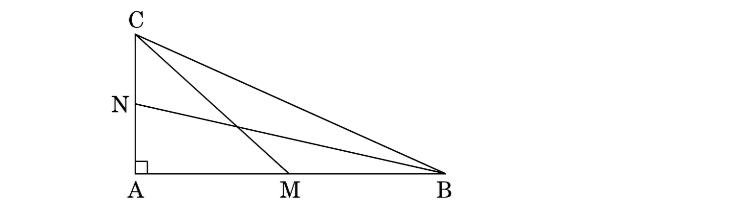
\includegraphics[width=\columnwidth]{cbse/figs/rightangled}
\caption{Right-angled triangle}
\label{fig:rightangled4}
\end{figure}

\hfill\brak{10, 2022}\item $\vec{Case Study - 1:}$
\begin{center}
$\vec{Kite Festival}$\\
\end{center}
Kite festival is celebrated in many countries at different times of the year. in India, every year 14th
January is celebrated as international kite Day. on his day many people visit India and participate in the festival by flying various kinds of kites.
\\The picture given below \figref{fig:kites5} , three kites flying together.
\begin{figure}[!ht]
\centering
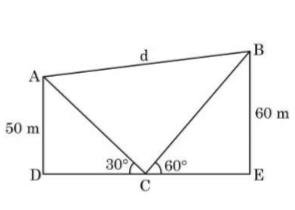
\includegraphics[width=\columnwidth]{cbse/figs/kites}
\caption{kites flying to gether}
\label{fig:kites5}
\end{figure}
\\In \figref{fig:kites5}, the angles of elevation of two kites (point C) are found to be $\degree{30}$ and  $\degree{60}$ respectively. Taking \begin{align}AD = 50 m\end{align} and\begin{align} BE = 60 m\end{align}
find
\begin{enumerate}
\item The length of string used (take them straight) for kites A and B as shown in the figure.
\item The distance 'd' between these two kites
\end{enumerate}
\hfill\brak{10, 2022}
\item Simplest form of 
 \begin{align}
     \frac{1 + \tan^{2}{A}}{1 + \cot^{2}{A}}
 \end{align}is .

\hfill\brak{10, 2020}\item Write the value of
 \begin{align}
	     \sin^{2}{30\degree} + \cos^{2}{60\degree}
	\end{align}.
\hfill\brak{10, 2020}\item If $A$, $B$ and $C$ are interior angles of $ \triangle ABC$, then show that
	\begin{align}
	    \cos \brak{\frac{B + C}{2}}=\sin \brak{\frac{A}{2}}
	\end{align}
      
\hfill\brak{10, 2020}\item Prove that : 
        \begin{align}
           (\sin^{4}{\theta} - \cos^{4}{\theta} + 1)\csc^{2}{\theta} = 2 
        \end{align}
\hfill\brak{10, 2020}
\item
If
\begin{align}
\cos\brak{\sin^{-1}{\frac{2}{\sqrt{5}}} + \cos^{-1}{x}} = 0
\end{align}
then $x$ is equal to
		\begin{multicols}{4}
\begin{enumerate}
	\item $\frac{1}{\sqrt{5}}$
	\item $-\frac{2}{\sqrt{5}}$
	\item $\frac{2}{\sqrt{5}}$
        \item $1$
\end{enumerate}
		\end{multicols}
\hfill\brak{12, 2020}
\item prove that \begin{align} \frac{\sin A-2 \sin^3A}{2\cos^3A-\cos A}=\tan A\end{align} 
  \hfill\brak{10, 2023}\item \begin{align} \sec A (1-\sin A)(\sec A+\tan A)=1\end{align} 

\hfill\brak{10, 2023}\item If 
\begin{align}
    4\cot^2 45\degree - \sec^2 60\degree + \sin^2 60\degree + p = \frac{3}{4}, 
\end{align}
then find the value of $p$.
\hfill\brak{10, 2023}\item If 
\begin{align}
    \cos A+ \cos^2A=1,
\end{align}then find the value of 
\begin{align}
\sin^2A+\sin^4A.
\end{align}
\hfill\brak{10, 2023}\item Prove that:\\
\begin{align}
\brak{\frac{1}{\cos\theta}-\cos\theta}\brak{\frac{1}{\sin\theta}-\sin\theta} = \frac{1}{\tan\theta+\cot\theta}
\end{align}




\hfill\brak{10, 2023}\item If $2\tan A=3$, then the value of $\frac{4sin A + 3\cos A}{4\sin A - 3\cos A}$ is
\begin{enumerate}
\item $\frac{7}{\sqrt{13}}$
\item $\frac{1}{\sqrt{13}}$
\item $3$
\item does not exist
\end{enumerate}



    \hfill\brak{10, 2023}\item $\brak{\sec^2\theta - 1}\brak{\csc^2\theta - 1}$  is equal to:
    \begin{enumerate}
   \item $-1$
   \item  $1$
   \item  $0$
   \item  $2$
        \end{enumerate}
   \hfill\brak{10, 2023}\item Evaluate $2\sec^2\theta+3\csc^2\theta-2\sin\theta\cos\theta$ if
   \begin{align}
      \theta=45\degree
   \end{align}
   
   \hfill\brak{10, 2023}\item If
   \begin{align}
       \sin\theta-\cos\theta=0
   \end{align}
   ,then find the value of $\sin^4\theta+\cos^4\theta$.
  \hfill\brak{10, 2023}
    \item If $\sin \theta=0$, then the value of $\tan^2\theta+\cot^2\theta$ is
    \begin{enumerate}
        \item $2$
        \item $4$
        \item $1$
        \item $\frac{10}{9}$
    \end{enumerate}
    \hfill\brak{10, 2022}\item $5\tan^2 \theta - 5\sec^2\theta = \underline{\hspace{2cm}}$
    \hfill\brak{10, 2022}\item In  \figref{fig:as.jpeg}, a tower stands vertically on the ground. From a point on the ground, which is $80m$ away from the foot of the tower, the angle of elevation of the tower is found to be $30\degree$. Find the height of the tower.
    \begin{figure}[H]
        \centering
        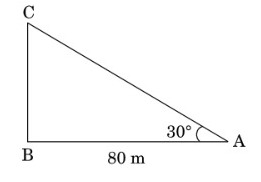
\includegraphics[width=70mm]{cbse/figs/as.jpeg}
        \caption{as.jpeg}
        \label{fig:as.jpeg}
    \end{figure}
    \hfill\brak{10, 2022}\item Show that 
    \begin{align}
        \cos(38\degree) \cos(52\degree) - \sin(38\degree)\sin(52\degree) = \cos(90\degree).
    \end{align}
    \hfill\brak{10, 2022}\item Prove that 
    \begin{align}
        \frac{\sin\theta}{\cot\theta+\csc\theta} = 2+\frac{\sin\theta}{\cot\theta-\csc\theta}.
    \end{align}
    \hfill\brak{10, 2022}\item Given 
    \begin{align}
        15 \cot (A) = 8,
    \end{align}
    find the values of $\sin (A)$ and $\sec (A)$.
    \hfill\brak{10, 2022}\item The angles of depression of the top and bottom of a tower as seen from the top of a $60\sqrt{3}m$ high cliff are $45\degree$ and $60\degree$ respectively. Find the height of the tower. (Use $\sqrt{3}=1.73$)
    \hfill\brak{10, 2022}\item The angle of elevation of the top of a building from the foot of the tower is $30\degree$ and the angle of elevation of the top of the tower from the foot of the building is $60\degree$. If the tower is $50$ meters high, then find the height of the building.
    \hfill\brak{10, 2022}\item From a point on a bridge across a river, the angles of depression of the banks on opposite sides of the river are $30\degree$ and $60\degree$ respectively. If the bridge is at a height of $3$ meters from the banks, then find the width of the river. 
    \hfill\brak{10, 2022}\item In \figref{fig:ak}, Gadisar Lake is located in the Jaisalmer district of Rajasthan. It was built by the King of Jaisalmer and rebuilt by Gadsi Singh in the $14$th century. The lake has many Chhatris. One of them is shown below:
    \begin{figure}[H]
        \centering
    	 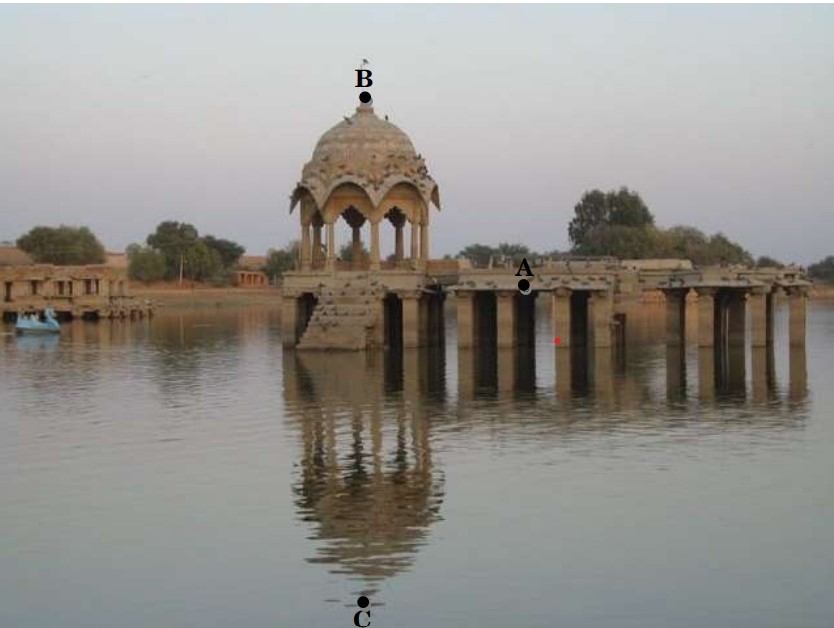
\includegraphics[width=70mm]{cbse/figs/ak.jpeg}
        \caption{ak.jpg}
        \label{fig:ak}
    \end{figure}
    Observe the picture. From a point $A$ $h$ meters above the water level, the angle of elevation of the top of Chhatri (point $B$) is $45\degree$ and the angle of depression of its reflection in the water (point $C$) is $60\degree$ . If the height of Chhatri above water level is (approximately) $10$ meters, then 
    \begin{enumerate}
        \item Draw a well-labeled figure based on the above information.
        \item Find the height ($h$) of the point $A$ above water level. (Use $\sqrt{3}=1.73$) 
    \end{enumerate}

    \hfill\brak{10, 2022}\item In \figref{fig:su.jpeg}, from a point on a bridge across a river, the angles of depression of the banks on opposite sides of the river are $30\degree$ and $45\degree$. If the bridge is at a height of $8$ meters from the banks, then find the width of the river.
    \begin{figure}[H]
        \centering
        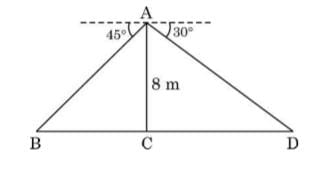
\includegraphics[width=70mm]{cbse/figs/su.jpeg}
        \caption{su.jpg}
        \label{fig:su.jpeg}
    \end{figure}
    
    \hfill\brak{10, 2022}\item Case Study-1:
    
    In \figref{fig:kite.jpeg}, Kite Festival is celebrated in many countries at different times of the year. In India, every year on $14^{th}$ January is celebrated as International Kite Day. On this day, many people visit India and participate in the festival by flying various kinds of kites.
    
    \begin{figure}[H]
	\centering
        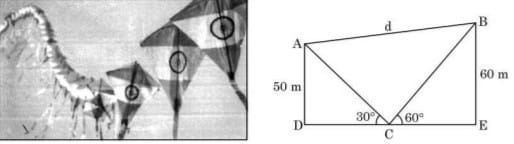
\includegraphics[width=70mm]{cbse/figs/kite.jpeg}
        \caption{kites}
        \label{fig:kite.jpeg}
    \end{figure}
    
    In Fig. 5, the angles of elevation of two kites (Point $A$ and $B$) from the hands of a man (Point $C$) are found to be $30\degree$ and $60\degree$ respectively. Taking $AD = 50$ meters and $BE = 60$ meters, find:
    \begin{enumerate}
        \item The lengths of strings used (take them straight) for kites $A$ and $B$ as shown in the figure.
        \item The distance $d$ between these two kites.
    \end{enumerate}
    
    \hfill\brak{10, 2022}\item Two boats are sailing in the sea $80$ meters apart from each other towards a cliff $AB$. The angles of depression of the boats from the top of the cliff are $30\degree$ and $45\degree$ respectively, as shown in \figref{fig:boat.jpeg}
    
    \begin{figure}[H]
        \centering
        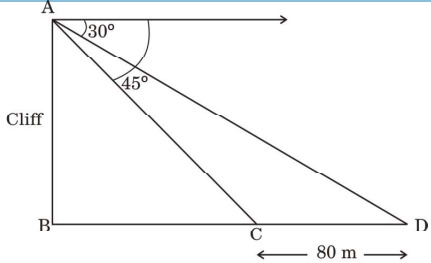
\includegraphics[width=70mm]{cbse/figs/boat.edit.jpeg}
        \caption{boat}
        \label{fig:boat.jpeg}
    \end{figure}
    
    Find the height of the cliff.
    
    \hfill\brak{10, 2022}\item The angle of elevation of the top $Q$ of a vertical tower $PQ$ from a point $X$ on the ground is $60\degree$. From a point $Y$, $40$ meters vertically above $X$, the angle of elevation of the top $Q$ of tower $PQ$ is $45\degree$. Find the height of the tower $PQ$ and the distance $PX$. (Use $\sqrt{3} = 1.73$)
    
    \hfill\brak{10, 2022}\item An Aeroplane at an altitude of $200$ meters observes the angles of depression of opposite points on the two banks of a river to be $45\degree$ and $60\degree$. Find the width of the river. (Use $\sqrt{3} = 1.732$)
    
    \hfill\brak{10, 2022}\item From the top of an $8$ meter high building, the angle of elevation of the top of a cable tower is $60\degree$ and the angle of depression of its foot is $45\degree$. Determine the height of the tower. (Take $\sqrt{3} = 1.732$).
    
    \hfill\brak{10, 2022}\item As observed from the top of a lighthouse $60$ meters high from the sea level, the angles of depression of two ships are $45\degree$ and $60\degree$. If one ship is exactly behind the other on the same side of the lighthouse, then find the distance between the two ships. (Use $\sqrt{3} = 1.732$)
    
    \hfill\brak{10, 2022}\item At a point on the level ground, the angle of elevation of the top of a vertical tower is found to be $\alpha$, such that $\tan\alpha = \frac{5}{12}$. On walking $192$ meters towards the tower, the angle of elevation $\beta$ is such that $\tan\beta = \frac{3}{4}$. Find the height of the tower.
    
    \hfill\brak{10, 2022}\item $\tan^{-1}\frac{1}{\sqrt{3}} - \cot^{-1}\frac{-1}{\sqrt{3}}$
    
    \hfill\brak{10, 2022}\item Two angles of a triangle are $\cot^{-1}2$ and $\cot^{-1}3$. The third angle of the triangle is?
    
    \hfill\brak{10, 2022}\item Solve for $x$:
    \begin{align}
        \sin^{-1}(1-x) - 2 \sin^{-1} x = \frac{\pi}{2}
    \end{align}
\hfill\brak{10, 2022}
\item If $2\cos  \theta = \sqrt{3}$ , then find the value of $\theta$
\hfill\brak{10, 2021}\item  In $\triangle ABC$, right-angled at $A$, if $AB=7 cm$ and $AC=24 cm$, then find $\sin B$
and $\tan C$.

\hfill\brak{10, 2021}\item If  $\sin (A+B) = \sqrt{3}/2,
 \sin (A-B) = 1/2,$ Where $0\degree<A+B<90\degree; A>B$, then find the values of $A$ and $B$.

\hfill\brak{10, 2021}\item  Simplify :
\begin{align}
\frac{\sin 30\degree + \tan 45\degree-\cos 60\degree}{\sec 30\degree + \cos 60\degree + \cot 45\degree} 
\end{align}


\hfill\brak{10, 2021}\item Prove that :
\begin{align}
 \sec \theta (1-\sin\theta)(\sec\theta+ \tan\theta)=1
\end{align}

\hfill\brak{10, 2021}\item Prove that :
\begin{align}
\frac{1+\sec A}{\sec A}=\frac{\sin^2 A}{1-\cos A} 
\end{align}

\hfill\brak{10, 2021}\item If  $\tan \theta = 4/3$, find the value 
$\frac{2\sin \theta -3\cos \theta}{2\sin\theta+3\cos\theta}$

\hfill\brak{10, 2021}\item If x=  $a\cos\theta$ and y=$b\sin\theta$, then find the value of   $b^2x^2+a^2y^2$

\hfill\brak{10, 2021}\item Prove that :
\begin{align}
\frac{\tan\theta-\cot\theta}{\sin\theta\cos\theta}=\tan^2\theta-\cot^2\theta 
\end{align}
\hfill\brak{10, 2021}\item Prove that:
\begin{align}
(\sec\theta-\tan\theta)^2 =\frac{1+\sin\theta}{1-\sin\theta}
\end{align}

		\hfill\brak{10, 2021}\item If $3\sin A = 1$, then find the value of $\sec A$.
		\hfill\brak{10, 2021}\item Show that: $\frac{1 + \cot^2{\theta}}{1 + \tan^2{\theta}} = \cot^2{\theta}$.
\hfill\brak{10, 2021}\item Simplify :$${\csc^{2}{60\degree} \sin^{2}{30\degree} - \sec^{2}{60\degree}}$$
	\hfill\brak{10, 2021}\item If $\tan{\theta} + \cot{\theta}$ = $\frac{4 \sqrt{3}}{3}$, then find the value of $\tan^{2}{\theta} + \cot^{2}{\theta}$. 
		\hfill\brak{10, 2021}\item Prove:$$\frac{1}{(\cot A)(\sec A) - \cot A} - \csc A = \csc A - \frac{1}{(\cot A)(\sec A) + \cot A}$$
		\hfill\brak{10, 2021}\item Prove:$$\sin^{6} A + 3\sin^{2} A \cos^{2} A = 1 - \cos^{6}  A$$
		\hfill\brak{10, 2021}\item A man on the top of a vertical tower observes a car moving at a uniform speed coming directly towards it. If it takes $18$ minutes for the angle of depression to change from $30\degree$ to $60\degree$, how soon after this will the car reach the tower ?

		\hfill\brak{10, 2021}\item A girl on a ship standing on a wooden platform, which is $50$ m above water level, observes the angle of elevation of a top of a hill as $30\degree$ and the angle of depression of the base of the hill as $60\degree$. Calculate the distance of the hill from the platform and the height of the hill.
\hfill\brak{10, 2021}
\item Two angles of a triangle are  $\cot^{-1}2$ and $\cot^{-1}3$.The third angle of the
triangle is \rule{30pt}{1pt}

\hfill\brak{12, 2021}\item Prove that $2\tan^{-1}\frac{1}{2} + \tan^{-1}\frac{1}{7} = \tan^{-1}\frac{31}{17}$

\hfill\brak{12, 2021}\item $ \sin \sbrak[\frac{\pi}{3}-\sin^{-1}(\frac{-1}{2})] $ is equal to:

\begin{enumerate}

\item $\frac{1}{2}$
\item $\frac{1}{3}$
\item -1
\item 1

\end{enumerate}

\hfill\brak{12, 2021}\item $ \sin(\tan^{-1}x)$,where $\abs{x} \le 1 $,is equal to:

\begin{enumerate}

\item$\frac{x}{\sqrt{1-x^2}}$
\item$\frac{1}{\sqrt{1-x^2}}$ 
\item$\frac{1}{\sqrt{1+x^2}}$
\item$\frac{x}{\sqrt{1+x^2}}$

\end{enumerate}  

\hfill\brak{12, 2021}\item Simplest form of $ \tan^{-1}(\frac{\sqrt{1+\cos x}+\sqrt{1-\cos x}}{\sqrt{1+\cos x}- \sqrt {1- \cos x}}) , \pi < x < \frac{3\pi}{2}$ is:

\begin{enumerate}

  \item$\frac{\pi}{4} - \frac{x}{2}$
  \item$\frac{3\pi}{2} - \frac{x}{2}$
  \item$-\frac{x}{2}$
  \item${\pi} - \frac{x}{2}$

\end{enumerate}
\hfill\brak{12, 2021}
\item Prove that 
\begin{align*}
    \sin^{-1}\frac{4}{5}+\tan^{-1}\frac{5}{12}+\cos^{-1}\frac{63}{65}=\frac{\pi}{2}
\end{align*}
\hfill\brak{12, 2019}
\item Find the value of $\sin\brak{\cos^{-1}{\frac{4}{5}}+{\tan^{-1}{\frac{2}{3}}}}$.
\hfill\brak{12, 2019}\item Solve for x:
\begin{align*}
\tan^{-1}\brak{x+1}+\tan^{-1}\brak{x-1}=\tan^{-1}\brak{\frac{8}{31}}
\end{align*}
\hfill\brak{12, 2019}\item Prove that :
\begin{align*}
\cos^{-1}\brak{\frac{12}{13}}+\sin^{-1}\brak{\frac{3}{5}}=\sin^{-1} \brak{\frac{56}{65}}
\end{align*}
\hfill\brak{12, 2019}

\item If $\tan^{-1}x-\cot^{-1}x =\tan^{-1}\brak{\frac{1}{ \sqrt3}}, x>0$ ,find the value of $x$ and hence find the value of $\sec^{-1}\left(\dfrac{2}{x}\right)$.

\hfill\brak{12, 2019}\item  If
\begin{align*}
 \sin^{-1} \brak{\dfrac{3}{x}} + \sin^{-1}\brak{\dfrac{4}{x}}=\dfrac{\pi}{2} 
\end{align*}
then find the value of $x$. 

\hfill\brak{12, 2019}\item Find the value of $x$, if $\tan \brak{\sec^{-1}\brak{\frac{1}{x}}} = \sin \brak{\tan^{-1}{2}},x > 0$.
\hfill\brak{12, 2019}

\item  Evaluate:
\begin{align*}
    \frac {\tan 65\degree}  {\cot 25\degree}
\end{align*}

\hfill\brak{10, 2019}\item Express $\brak{{\sin 67\degree}+ {\cos 75\degree}}$ in terms of trigonometric ratios of the angle between $0\degree$ and $45\degree$.

\hfill\brak{10, 2019}\item Prove that :
\begin{align*}
    \brak{\sin \theta+1+\cos \theta} \brak{\sin\theta-1+\cos\theta}.\sec\theta \csc\theta=2
\end{align*}

\hfill\brak{10, 2019}\item Prove that :
\begin{align*}
      \sqrt{\frac{\sec\theta-1}{\sec\theta+1}} + \sqrt{\frac{\sec\theta+1}{\sec\theta-1}} = 2\csc\theta
\end{align*}

\hfill\brak{10, 2019}\item If $\sec\theta + \tan\theta=m$, show that $\frac{m^2-1}{m^2+1} = \sin\theta$.

\hfill\brak{10, 2019}\item Prove that :
\begin{align*}
    2 (\sin^6\theta +\cos^6\theta) - 3 (\sin^4\theta + \cos^4\theta) + 1 = 0
\end{align*}

\hfill\brak{10, 2019}\item Find $A$ and $B$ if $\sin \brak{A + 2B}=\frac{\sqrt{3}}{2}$ and $\cos \brak{A + 4B} = 0$, where $A$ and $B$ are acute angles.





\hfill\brak{10, 2019}\item Evaluate :
 \begin{align*}
	     \sin^{2}{60\degree} + 2\tan{45\degree} - \cos^{2}{30\degree}. 
      \end{align*}

\hfill\brak{10, 2019}\item Evaluate :
\begin{align*}
\left(\frac{3\tan 41\degree}{\cot 90\degree}\right)^2 - \left(\frac{\sin 3\degree \sec 55\degree}{\tan 10\degree \tan 20\degree \tan 60\degree \tan 70\degree \tan 80\degree}\right)^2
\end{align*}

\hfill\brak{10, 2019}\item Prove that :
\begin{align*}
\frac{\tan \theta}{1-\cot \theta} + \frac{\cot \theta}{1- \tan \theta} = 1+ \sec \theta  \csc  \theta   
\end{align*}

\hfill\brak{10, 2019}\item Prove that :
\begin{align*}
    \frac{\sin \theta}{\cot \theta + \csc \theta} = 2 + \frac{\sin \theta}{\cot \theta - \csc \theta}
\end{align*}

\hfill\brak{10, 2019}\item Evaluate :
\begin{align*}
\left(\frac{3\sin 43\degree}{\cos 47\degree}\right)^2 - \frac{\cos 37\degree \csc 53\degree}{\tan 5\degree \tan 25\degree \tan 45\degree \tan 65\degree \tan 85\degree}
\end{align*}


 \hfill\brak{10, 2019}\item If $\sin A = \frac{3}{4}$, calculate $\sec A$.


\hfill\brak{10, 2019}\item If $\tan$ $\alpha$ = ${\frac {5}{12}}$, find the value of $\sec$ $\alpha$.

\hfill\brak{10, 2019}\item $A$, $B$ and $C$ are interior angles of a triangle $ABC$. Show that
\begin{enumerate}
\item  $\sin$ $ \brak{{\frac {B+C}{2}}} = \cos {\frac {A}{2}}$
\item  If $\angle A = 90 \degree$ , then find the value of $\tan \brak{{\frac{B+C}{2}}}$ 
\end{enumerate} 

\hfill\brak{10, 2019}\item If $\tan \brak{A + B} = 1$ and $\tan \brak{A - B} = \frac{1}{\sqrt{3}}$ , $0\degree$ $<$ $A + B$ $<$ $90\degree$, $A > B$, then find the values of $A$ and $B$.

\hfill\brak{10, 2019}\item If $1 + \sin^2 \theta  = 3 \sin \theta \cos \theta$, then prove that $\tan$ $\theta = 1 $ or $\tan$ $\theta = \frac{1}{2}$

\hfill\brak{10, 2019}\item Prove that :
\begin{align*}
\frac{\tan^3 \theta}{1+\tan^2 \theta} + \frac{\cot^3 \theta}{1 + \cot^2 \theta} =  \sec \theta  \csc  \theta - 2 \sin \theta \cos \theta  
\end{align*}


\hfill\brak{10, 2019}\item If $\sin{x} + \cos{y}= 1$ ; $x=30\degree$  and  $y$ is an acute angle, find the value of $y$ .

\hfill\brak{10, 2019}\item Find the value of $\cos {48\degree} - \sin {42\degree}$.

\hfill\brak{10, 2019}\item Prove that :
\begin{align*}
   {\frac{\tan\theta}{1-\tan\theta}} - {\frac{\cot\theta}{1-\cot\theta}}={\frac{\cos\theta+ \sin\theta}{\cos\theta-\sin\theta}}
\end{align*} 

\hfill\brak{10, 2019}\item If ${\cos\theta + \sin\theta} = {\sqrt 2}{\cos\theta}$, show that ${\cos\theta - \sin\theta} = {\sqrt 2}{\sin\theta}$.

\hfill\brak{10, 2019}\item Prove that :
\begin{align*}
    {\frac{(1+\cot\theta+\tan\theta)(\sin\theta-\cos\theta)}{(\sec^3\theta-\csc^3\theta)}} = \sin^2\theta \cos^2\theta
\end{align*}

\hfill\brak{10, 2019}\item Evaluate :
\begin{align*}
    {\frac{\csc^2(90\degree - \theta)-\tan^2\theta)}{2(\cos^2 37\degree + \cos^2 53\degree)}} - {\frac{2\tan^2 30\degree \sec^2 37\degree \cdot \sin^2 53\degree}{\csc^2 63\degree - \tan^2 27\degree}} 
\end{align*}	




  \hfill\brak{10, 2019}\item Prove that \begin{align*} \brak{\sin\theta + \csc\theta}^2 + \brak{\cos\theta + \sec\theta}^2 = 7 + \tan^2\theta + \cot^2\theta\end{align*}.
  \hfill\brak{10, 2019}\item Prove that \begin{align*}\brak{1+\cot A - \csc A} \brak{1 + \tan A +\sec A} = 2 \end{align*}.
  \hfill\brak{10, 2019}\item Prove that \begin{align*} \frac{\sin A-\cos A+1}{\sin A+ \cos A-1} =\frac{1}{\sec A-\tan A}\end{align*}
  \hfill\brak{10, 2019}\item Find $A$ if \begin{align*}\tan 2A = \cot (A-24\degree)\end{align*}
  \hfill\brak{10, 2019}\item Find the value of \begin{align*}(\sin^2 33\degree+ \sin^2 57\degree)\end{align*}
  
  
  \hfill\brak{10, 2019}\item if If $\sec\theta = x + \frac{1}{4x}$, where $x \neq 0$, find $(\sec\theta + \tan\theta)$.
  \hfill\brak{10, 2019}\item prove that \begin{align*} \frac{\tan^2A}{\tan^2 A-1}+\frac{\csc^2 A}{\sec^2 A-\csc^2 A}=\frac{1}{1-2\cos^2 A}\end{align*}
\hfill\brak{10, 2019}
\item If $4$ $\tan\theta=3$, evaluate \begin{align*}\brak {\frac{4 \sin\theta - \cos\theta + 1 }{ 4 \sin\theta + \cos\theta - 1 } } \end{align*}   

\hfill\brak{10, 2018}\item If $\tan2A = \cot(A-18\degree)$, where $2A$ is an acute angle, find the value of $A$.

\hfill\brak{10, 2018}\item What is the value of $ \brak{\cos^2 67\degree - \sin^2 23\degree}$ ?

\hfill\brak{10, 2018}\item  Prove that:$\brak{\frac{\sin A - 2sin^3 A}{2 \cos^3 A-\cos A} = \tan A }$

			\hfill\brak{10, 2018}
\item Find the value of
	\begin{align*}
		\tan^{-1}\sqrt{3}-\cot^{-1}\brak{\sqrt{-3}}
	\end{align*}
 \hfill\brak{12, 2018}\item Prove that 
			\begin{align*}
		3\sin^{-1}x=\sin^{-1}\brak{3x-4x^3}, x\in\brak{\frac{-1}{2},\frac{1}{2}}
			\end{align*} 

\hfill\brak{12, 2018}\item Prove that :
	\begin{align*}
		\cos^{-1}\brak{\frac{12}{13}}+\sin^{-1}\brak{\frac{3}{5}}=\sin^{-1} \brak{\frac{56}{65}}
	\end{align*}
 \hfill\brak{12, 2018}\item Prove that :
         \begin{align}
          \sin^{-1}\brak{\dfrac{8}{17}}+\cos^{-1}\brak{\dfrac{4}{5}}=\cot^{-1}\brak{\dfrac{36}{77}}
         \end{align}

\hfill\brak{12, 2018}\item Prove that :
    \begin{align*}
       \sin^{-1}\dfrac{4}{5}+\tan^{-1}\dfrac{5}{12}+\cos^{-1}\dfrac{63}{65}=\dfrac{\pi}{2}
    \end{align*}

\hfill\brak{12, 2018}\item If $\tan^{-1}{x} - \cot^{-1} {x}= tan^{-1}\brak{\frac{1}{\sqrt{3}}},$ $x > 0,$ find the value of $x$ and hence find the value of $\sec^{-1}\brak{\frac{2}{x}}$.
 \hfill\brak{12, 2018}\item If $\sin^{-1}\brak{\frac{3}{x}} + \sin^{-1}\brak{\frac{4}{x}} = \frac{\pi}{2}$, then find the value of $x$.
 \hfill\brak{12, 2018}\item Find  the value of $x$, if $\tan\brak{\sec^{-1}\brak{\dfrac{1}{x}}}  = \sin \brak{\tan^{-1}{2}},x>0$.

\hfill\brak{12, 2018}
\item Find the value of $\sin\brak{\cos^{-1}{\frac{4}{5}}+{\tan^{-1}{\frac{2}{3}}}}$
\hfill\brak{12, 2018}\item Solve for $x$:
	\begin{align*}
	\tan^{-1}\brak{x+1}+\tan^{-1}\brak{x-1}=\tan^{-1}\brak{\dfrac{8}{31}}
	\end{align*}
\hfill\brak{12, 2018}
\item Solve : $\tan^{-1}4x+\tan^{-1}6x=\frac{\pi}{4}$
\hfill\brak{12, 2018}
\item Solve for x :  $\tan^{-1}(2x)+\tan^{-1}(3x)=\frac{\pi}{4}$
\hfill\brak{12, 2018}

\item if $\tan^{-1}\dfrac{x-3}{x-4} + \tan^{-1}\dfrac{x+3}{x+4} =\dfrac{\pi}{4}$, then find the value of $x$ .
\hfill\brak{12, 2017}

	\item Prove that $ 2\sin^{-1} \brak{\frac{3}{5}} - \tan^{-1} \brak{\frac{17}{31}} = \frac{\pi}{4}$

	\hfill\brak{12, 2016}\item Solve the equation for $x$: $\cos (\tan^{-1}) = \sin \brak{\cot^{-1} \frac{3}{4}} = \sin \brak{\cot^{-1} \frac{3}{4}}$

	
	\hfill\brak{12, 2016}\item Solve for 
	\begin{align*}
		x: \tan^{-1}(x-1) + \tan^{-1}x + \tan^{-1}(x+1) = \tan^{-1}3x
	\end{align*}

	\hfill\brak{12, 2016}\item Prove that 
	\begin{align*}
	\tan^{-1} \brak{\frac{6x-8x^{3}}{1-12x^{2}}} - \tan^{-1} \brak{\frac{4x}{1-4x^{2}}} = \tan^{-1}2x;
	\end{align*}
	\begin{align*}
		\abs{2x} < \frac{1}{\sqrt{3}}
	\end{align*}

 	\hfill\brak{12, 2016}\item Prove that 
	\begin{align*}
		2\sin^{-1}\brak{\frac{3}{5}}-\tan^{-1}\brak{\frac{17}{31}} = \frac{\pi}{4}
	\end{align*}
	\hfill\brak{12, 2016}\item Solve the equation for x:
	\begin{align*}
	\cos\brak{\tan^{-1}x} = \sin\brak{\cot^{-1}\frac{3}{4}}
	\end{align*}
\hfill\brak{12, 2016}
\item Prove that $2\tan^{-1}\brak{\frac{1}{2}}+\tan^{-1}\brak{\frac{1}{7}} = \sin^{-1}\brak{\frac{31}{25\sqrt{2}}}$. 

\hfill\brak{12, 2015}\item Solve for x: $\tan^{-1}\brak{\frac{1-x}{1+x}} = \frac{1}{2}\tan^{-1}x$, $x>0$. 
\hfill\brak{12, 2015}
\item The length of the shadow of a tower on the plane ground is $\sqrt{3}$ times the height of the tower.Find the angle of elevation of the sun.

\hfill\brak{10, 2023}\item  The angle of elevation of the top of a tower from a point on the ground which is $30$ m away from the foot of the tower,is $30\degree$ .Find the height of the tower.

\hfill\brak{10, 2023}\item  As observed from the top of a $75$ m high lighthouse from the sea-level,the angles of depression of two ships are $30\degree$ and $60\degree$.If one ship is exactly behind the other on the same side of the lighthouse,find the distance between two ships.$\brak{Use \sqrt{3} = 1.73}$

\hfill\brak{10, 2023}\item  From a point on the ground,the angle of elevation of the bottom and top of a transmission tower fixed at the top of $30$ m high building are $30\degree$ and $60\degree$, respectively.Find the height of the transmission tower.$\brak{Use \sqrt{3} = 1.73}$
 \hfill\brak{10, 2023}   

\item A straight highway leads to the foot of a tower.A man standing on the top of the $75$ m high tower observes two cars at angles of depression of $30\degree$ and $60\degree$,Which are approaching the foot of the tower.If one car is exactly behind the other on the same side of the tower,find the distance between the two cars.
    \hfill\brak{10, 2023}\item From the top of a $7$ m high building, the angle of elevation of the top of a cable tower is $60\degree$ and the angle of depression of its foot is $30\degree$.Determine the height of the tower.(take $\sqrt{3}=1.73$)
\hfill\brak{10, 2023}\item The angle of elevation of the top of a tower $24$ m high from the foot of another tower in the same plane is ${60}{\degree}$. The angle of elevation of the top of second tower from the foot of the first tower is ${30}{\degree}$. Find the distance between two towers and the height of the other tower. Also, find the length of the wire attached to the tops of both the towers.
\hfill\brak{10, 2023}\item A spherical balloon of radius $r$ subtends an angle of ${60}{\degree}$ at the eye of an observer. If the angle of elevation of its centre is ${45}{\degree}$ from the same point, then prove that height of the centre of the balloon is $\sqrt{2}$ times its radius.
    \hfill\brak{10, 2023}

\item A vertical pole is $100$ metres high. Find the angle subtended by the pole at a point on
the ground $100 \sqrt{3}$ meters from the base of the pole.

    \hfill\brak{10, 2021}\item The angle of elevation of the top of a tower from a point is found to be $60\degree$.At a point $40$ m above the first point, the angle of elevation of the top of the tower is $45\degree$.Find the height of the tower.
    \hfill\brak{10, 2021}\item A statue $1.6$m tall stands on the top of a pedestal. From a point on the ground, the angle of elevation of the top of statue is $60\degree$ and from the same point, the angle of elevation of the top of the pedestal is $45\degree$.Find the height of the pedestal.
    \hfill\brak{10, 2021}\item Two poles, $6$m and $11$ m high, stand vertically on the ground. If the distance between their feet is $12$ m, find the distance between their tops.

	\hfill\brak{10, 2021}\item The angle of elevation of the top of a tower from a point on the ground,which is $30$ m away from the foot of the tower is $45\degree$ .What is the height of the tower ?
	\hfill\brak{10, 2021}\item Find the sun's altitude if the shadow of a 15 m high tower is ${15}\sqrt{3}$ m.
	\hfill\brak{10, 2021}\item From a point on the ground, $20$ m away from the foot of vertical tower, the angle of elevation of the top of the tower is $60\degree$. Find the height of the tower.
			\hfill\brak{10, 2021}\item In $\triangle$ $ABC$, $AB = {4\sqrt{3}}$ cm, $AC = 8 cm$ and $BC = 4 cm$. The angle $B$ is
				\begin{enumerate}
\item $120\degree$
\item $90\degree$
\item $60\degree$
\item $45\degree$
				\end{enumerate}
	\hfill\brak{10, 2021}\item To explain how trignometry can be used measure the height of an inaccessible object, a teacher gave the following example to students :

		A TV tower stands vertically n the bank of a canal. From a point on the other bank direct opposite the tower, the angle of the elevation of the top of the tower is $60\degree$.From another point 20 m away from this point to the foot of the tower, the angle of elevation of the top of the tower is $30\degree$ (as shown in Figure 1).

		\begin{figure}[H]
			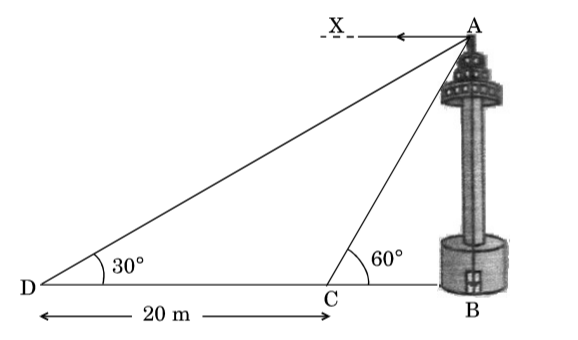
\includegraphics[width=0.75\columnwidth]{cbse/figs/Problem.png}
			\caption{Projection of Tower}
			\label{fig:traingle}
		\end{figure}
		Based on the above, answer the following questions :
		\begin{enumerate}
			\item The width of the canal is
				\begin{enumerate}
					\item ${10}\sqrt{3} m$
					\item ${20}\sqrt{3} m$
					\item $10 m$
					\item $20 m$
				\end{enumerate}
			\item Height of the tower is
				\begin{enumerate}
					\item ${10}\sqrt{3} m$
					\item $10 m$
					\item ${20}\sqrt{3} m$
					\item $20 m$
				\end{enumerate}
			\item Distance of the foot of the tower from the point $D$ is
				\begin{enumerate}
					\item $20 m$
					\item $30 m$
					\item $10 m$
					\item ${20}\sqrt{3} m$
				\end{enumerate}
\end{enumerate}
\hfill\brak{10, 2021}
\item In \figref{fig:Fig-4.png}, the angle of elevation of the top of a tower from a point $C$ on the ground, which is $30m$ away from the foot of the tower, is $30\degree$. Find the height of the tower.      
\begin{figure}[H]
\centering
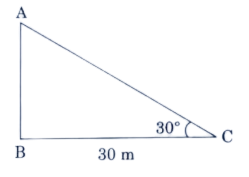
\includegraphics[width=0.75\columnwidth]{cbse/figs/Fig-4.png}
\caption{}      
\label{fig:Fig-4.png}
\end{figure}
\hfill\brak{10, 2020}\item A statue $1.6m$ tall, stands on the top of a pedestal. From a point on the ground, the angle of elevation of the top of the statue is $60\degree$ and from the same point the angle of elevation of the top of the pedestal is $45\degree$. Find the height of the pedestal.(Use $\sqrt{3}=1.73$)
\hfill\brak{10, 2020}
\item A moving boat is observed from the top of a $150m$ high cliff moving away from the cliff. The angle of depression of the boat changes from $60\degree$ to $45\degree$ in $2$ minutes. Find the speed of the boat in m/min.

\hfill\brak{10, 2019}\item There are two poles, one each on either bank of a river just opposite to each other. One pole is $60m$ high. From the top of this pole, the angle of depression of the top and foot of the other pole are $30\degree$ and $60\degree$respectively. Find the width of the river and height of the other pole.

\hfill\brak{10, 2019}\item Two poles of equal heights are standing opposite to each other on either side of the road which is $80 m$ wide. From a point $P$ between them on the road, the angle of elevation of the top of a pole is $60\degree$ and the angle of depression from the top of the other pole of point $P$ is $30\degree$. Find the heights of the poles and the distance of the point $P$ from the poles.

\hfill\brak{10, 2019}\item Amit, standing on a horizontal plane, finds a bird flying at a distance of $200 m$ from him at an elevation of $30\degree$. Deepak standing on the roof of a $50 m$ high building, finds the angle of elevation of the same bird to be $45\degree$. Amit and Deepak are on opposite sides of the bird. Find the distance of the bird from Deepak.

\hfill\brak{10, 2019}\item From a point $P$ on the ground, the angle of elevation of the top of a tower is $30\degree$ and that of the top of the flag-staff fixed on the top of the tower is $\sqrt{5}$. If the length of the flag-staff is $5 m$, find the height of the tower. (Use $\sqrt{3}= 1.732$).


\hfill\brak{10, 2019}\item The shadow of a tower standing on a level ground is found to be $40 m$ longer when the Sun's altitude is $30\degree$ than when it was $60\degree$. Find the height of the tower. $(Given \sqrt{3} = 1.732)$

\hfill\brak{10, 2019}\item A man in a boat rowing away from a light house $100m$  high takes $2$ minutes to change the angle of elevation of the top of the light house from $60\degree$ to $30\degree$. Find the speed of the boat in metres per minute. [Use $\sqrt{3}=1.732$]
\hfill\brak{10, 2019}\item Two poles of equal heights are standing opposite each other on either side of the road, which is $80 m$  wide. From a point between them on the road, the angles of elevation of the top of the poles are $60\degree$ to $30\degree$ respectively. Find the height of the poles and the distances of the point from the poles.
\hfill\brak{10, 2019}
		\item As observed from the top of a $100 m$ high light house from the sea level, the angles of depression of two ships are $30\degree$ and $45\degree$. If one ship is exactly behind the other on the same side of the light house, find the distance between the two ships. ({\textbf{Use}} $\sqrt3 = 1.732$)
\hfill\brak{10, 2018}
\item A statue, $1.46$m tall, stands on a pedestal. From a point on the ground the angle of elevation of the top of the statue is $60\degree{}$ and from the same point angle of elevation of the top of the pedestal is $45\degree{}$. Find the height of the pedestal. $\brak{use \sqrt{3}=1.73}$
\hfill\brak{10, 2018}
\item A ladder, leaning against a wall, makes an angle of $60 \degree$ with the horizontal.If the foot of the ladder is $2.5$ m away from the wall, find the length of the ladder.\\
\hfill\brak{10, 2016}\item  A man standing on the deck of a ship, which is $10$ m above water level, observes the angle of elevation of the top of a hill as $ 60\degree $ and the angle of depression of the base of hill as $ 30 \degree $. Find the distance of the hill from the ship and the height of the hill.\\
\hfill\brak{10, 2016}\item The angle of elevation of the top $Q$ of a vertical tower $PQ$ from a point $X$ on the ground is $ 60\degree $. From a point $Y$, $40$ m vertically above $X$, the angle of elevation of the top $Q$ of tower is $ 45 \degree $. Find the height of the tower $PQ$ and the distance $PX$. $\brak{\text{Use }\sqrt{3} = 1.73}$\\
\hfill\brak{10, 2016}
\item A boy standing on a horizontal plane finds a bird flying at a distance of $100 m$ from him at an elevation of $30\degree$. A girl standing on the roof of a $20 m$ high building, finds the elevation of the same bird to be $45\degree$. The boy and the girl are on the opposite sides of the bird. Find the distance of the bird from the girl. (Given ${\sqrt 2}= 1.414$)

\hfill\brak{10, 2019}\item The angle of elevation of an aeroplane from a point $A$ on the ground is $60\degree$. After a flight of $30 $seconds , the angle of elevation changes to $30\degree$. If the plane is flying at a constant height of $3600\sqrt 3 $ metres, find the speed of the aeroplane.

\hfill\brak{10, 2019}
\item If $\sin\theta+\cos\theta=\sqrt{2}\cos\brak{90\degree{}-\theta}$, find the value of $\cot\theta$.
\hfill\brak{10, 2018}\item Prove that : $\dfrac{1}{\cosec\theta+\cot\theta}-\dfrac{1}{\sin\theta}=\dfrac{1}{\sin\theta}-\dfrac{1}{\cosec\theta-\cot\theta}$
\hfill\brak{10, 2018}\item If $\tan\theta+\sin\theta=m$, $\tan\theta-\sin\theta=n$, show that $m^{2}-n^{2}=4\sqrt{mn}$
\hfill\brak{10, 2018}\item Prove that : $\brak{\dfrac{\sin A}{1-\cos A}-\dfrac{1-\cos A}{\sin A}}.\brak{\dfrac{\cos A}{1-\sin A}-\dfrac{1-\sin A}{\cos A}}=4$.
\hfill\brak{10, 2018}
\item If a tower $30$ m high, casts a shadow $10\sqrt{3}$ m long on a ground, then what is the angle of elevation of the sun ?
\hfill\brak{10, 2017}\item A man observes a car from the top of a tower, which is  moving towards the tower with a uniform speed. If the angle of depression of the car changes from $30\degree$ to $45\degree$ in $12$ minutes, find the time taken by the car now to reach the tower.
\hfill\brak{10, 2017}\item An aeroplane is flying at a height of $300 m$ above the ground. Flying at this height, the angles of depression from the aeroplane of two points on both banks of a river in opposite directions are $45\degree$ and $60\degree$ respectively. Find the width of the river. 
\hfill $\sbrak{Use \sqrt 3 = 1.732}$
\hfill\brak{10, 2017}\item On a straight line passing through the foot of a tower, two points $C$$D$ are at distances of $4$ m
and $16$ m from the foot respectively. If the angles of elevation from$C$$D$ of the top tower are complementary, then find the height of the tower.  
\hfill\brak{10, 2017}\item From the top of a tower, $100$ m high, a man observes two cars on the opposite sides of the tower and in same straight line with its base, with angles of depression $30\degree$ and $45\degree$. Find the distance between the cars.
\hfill  $\sbrak{Take \sqrt{3} = 1.732}$
\hfill\brak{10, 2017}

\item Solve for $x$: $\tan^{-1}(x-1) + \tan^{-1}x + \tan^{-1}(x+1) = \tan^{-1}3x$.
\hfill\brak{12, 2016}\item Prove that $\tan[\frac{6x-8x^3}{1-12x^2}]-\tan^{-1}[\frac{4x}{1-4x^2}]=\tan^{-1}2x:|2x|<\frac{1}{\sqrt{3}}$
\hfill\brak{12, 2016}\item Solve for x: $tan^{-1}(\frac{2-x}{2+x}) = \frac{1}{2} tan^{-1}\frac{x}{2},x>0$
\hfill\brak{12, 2016}
\item At a point $A$, $20$ metres above the level of water in a lake, the angle of elevation of a cloud is $30 \degree.$ The angle of depression of the reflection of the cloud in the lake, at $A$ is $60\degree .$ Find the distance of the cloud from $A$.
\hfill\brak{10, 2015}\item In Figure \ref{Figure 1}, a tower $AB$ is $20$ m high and $BC$, its shadow on the ground,is $20\sqrt{3}$ m long. Find the sun's altitude.
\begin{figure}[h!]
	\centering
    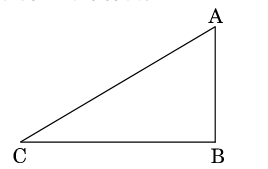
\includegraphics[width=\columnwidth]{cbse/figs/cbse_30_3_1.png}
	\caption{}
	\label{Figure 1}
\end{figure}
\hfill\brak{10, 2015}\item The angle of elevation of an aeroplane from a point $A$ on the ground is $60 \degree  $. After a flight of $15$ seconds, the angle of elevation changes to $  30 \degree.$ If the aeroplane is flying at a constant height of $1500\sqrt{3}$ m, find the speed of the plane in km/hr.
\hfill\brak{10, 2015}
\item A kite is flying at a height of $30 \text{ m}$ from the ground. The length of string from the kite to the ground is $60 \text{ m}$. Assuming that there is no slack in the string, the angle of elevation of the kite at the ground is 
\hfill\brak{10, 2012}\item From a point on the ground, which is $15\text{ m}$ away from the foot of a vertical tower, the angle of elevation of the top of the tower, is found to be $60\degree$. The height of the tower in $\brak{\text{in metres}}$ is 
\hfill\brak{10, 2012}\item The length of shadow of a tower on the plane ground is $\sqrt 3 \text{ m}$ times the height of the tower. The angle of elevation of sun is : 
\hfill\brak{10, 2012}\item The angles of depression of the top and bottom of a tower as seen from the top of a $60\sqrt 3 \text{ m}$ high cliff are $45\degree$ and $60\degree$ respectively. Find the height of the tower. 
%Trigonometry
\hfill\brak{10, 2012}\item In a flight of $2800 \text{ km}$, an aircraft was slowed down due to bad weather. Its average speed is reduced by $100 \text{ km/h}$ and time is increased by $30$ minutes. Find the original duration of flight. 
%Trigonometry
\hfill\brak{10, 2012}\item The angles of elevation and depression of the top and bottom of a light-house from the top of a $60 \text{ m}$ high building are $30\degree$ and $60\degree$ respectively. Find 
\begin{enumerate}
\item the difference between the heights of the light-house and the building. 
\item the distance between light-house and building. 
\end{enumerate}
%trigonometry
\hfill\brak{10, 2012}\item The angles of depression of two ships from the top of a light house and on the same side of it are found to be $45\degree$ and $30\degree$. if the ships are $200 \text{ km}$ apart, find the height of the light house. 
\hfill\brak{10, 2012}\item The angle of elevation of the top of a hill at the foot of a tower is $60\degree$ and the angle of depression from the top of the tower of the foot of the hill is $30\degree$. If the tower is $50\text{ m}$ high, find the height of the hill. 
\hfill\brak{10, 2012}\item From the top of a tower $50\text{ m}$ high, the angle of depression of the top of a pole is $45\degree$ and from the foot of the pole, the angle of elevation of the top of the tower is $60\degree$. find the height of the pole if the pole and tower stand on the same plane. 
\hfill\brak{10, 2012}\item The angle of depression from the top of a tower of a point $A$ on the ground is $30\degree$. On moving a distance of $20\text{ m}$ from the point $A$ towards the foot of the tower to a point $B$ the angle of elevation of the top of the tower from point $B$ is $60\degree$. Find the height of the tower and its distance from point $A$.
\hfill\brak{10, 2012}
\item A tower stands vertically on the ground. From a point on the ground which is $25$ m away from the foot of the tower, the angle of elevation of the top of the tower is found to be $45\degree$. Then the height $\brak{in\,meters}$ of the tower is



\hfill\brak{10, 2011}\item The angle of elevation of the top of a vertical tower from a point on the ground is $60\degree$. From another point $10$ m vertically above the first, its angle of elevation is $30\degree$. Find the height of the tower.


\hfill\brak{10, 2011}\item From the top of a vertical tower, the angles of depression of two cars, in the same straight line with the base of the tower, at an instant are found to be $45\degree$ and $60\degree$. If the cars are $100$ m apart and are on the same side of the tower, find the height of the tower. 

[Use $\sqrt{3} = 1.73$]
\hfill\brak{10, 2011}
    \item The angle of elevation of the top of a tower from a point on the ground, which is 30 m away from the foot of the tower is 45°. The height of the tower (in metres) is
    \hfill\brak{10, 2011}\item From the top of a tower $100$ $m$ high, a man observes two cars on the opposite sides of the tower with angles of depression $30^\circ$ and $45^\circ$ respectively. Find the distance between the cars. [Use $\sqrt{3}=1.73$].
    \hfill\brak{10, 2011}\item Two poles of equal heights are standing opposite to each other on either side of the road, which is $100m$ wide. From a point between them on the road, the angles of elevation of the top of the poles are $60^\circ$ and $30^\circ$, respectively. Find the height of the poles.
\hfill\brak{10, 2011}


\item Write the principal value of $\sec^{-1} \brak{-2}$.

\hfill\brak{12, 2010}\item Prove the following:
    \begin{align*}
        \cos \sbrak{\tan^{-1} \cbrak{\sin \brak{cot^{-1} x}}} = \sqrt{\frac{1 + x^2}{2 + x^2}}
    \end{align*}

\hfill\brak{12, 2010}\item Prove the following:
    \begin{align*}
        \tan^{-1} x + \tan^{-1} \brak{\frac{2x}{1 - x^2}} = \tan^{-1} \brak{\frac{3x - x^3}{1 - 3x^2}}
    \end{align*}
\hfill\brak{12, 2010}
\item A man standing on the deck of a ship, which is 10 m above the water level, observes the
angle of elevation of the top of a hill as 60° and the angle of depression of the base of the hill as
300. Calculate the distance of the hill from the ship and the height of the hill.

\hfill\brak{10, 2006}\item From a window $x$ meters high above the ground in a street, the angles of elevation and depression of the top and foot of the other house on the opposite side of the street are $\alpha$ and $\beta$ respectively. Show that the height of the opposite house is $x(1 + \tan \alpha \cot \beta)$ meters.

\hfill\brak{10, 2006}
\item Find the value of $\tan^{-1} (-\frac{1}{\sqrt{3}}) + \cot^{-1}(\frac{1}{\sqrt{3}}) + \tan^{-1}[\sin(-\frac{\pi}{2})]$
	 \hfill\brak{10, 2024}
\item If $\sec\theta - \tan\theta = m$, then the value of $\sec\theta + \tan\theta$ is:

 \hfill\brak{10, 2024}\item If $\cos(\alpha + \beta) = 0$ then the value of $\cos\left(\frac{\alpha + \beta}{2}\right)$ is equal to:
hfill\brak{10, 2024}

\item Simplify: $\cos^{-1}x + \cos^{-1}\sbrak{\frac{x}{2}{\frac{\sqrt{3-3x^2}}{2}}};-\frac{1}{2} \leq x \leq 1$

\hfill\brak{12, 2024}\item\textbf{ Evaluate:} $2\sqrt{2} \cos 45\degree \sin 10\degree + 2\sqrt{3} \cos 30\degree$

\hfill\brak{10, 2024}\item If  $A = 60\degree$ and  $B = 30\degree$, verify that : $\sin\brak{A + B} = \sin A \cos B + \cos A \sin B$

\hfill\brak{10, 2024}\item Prove that : $\frac{\tan{\theta}}{1 - \cot{\theta}} + \frac{\cot{\theta}}{1 - \tan{\theta}} = 1 + \sec
{\theta}\csc{\theta}$
\hfill\brak{10, 2024}\item A pole $6m$ high is fixed on the top of a tower. The angle of elevation of the top of the pole observe
d from a point $P$ on the ground is $60\degree$ and the angle of depression of the point $P$ from the top of
 the tower is $45\degree$. Find the height of the tower and the distance of point $P$ from the foot of the t
ower
\hfill\brak{10, 2024}

\item If $ a = \sin^{-1}\left(\frac{\sqrt{2}}{2}\right) + \cos^{-1}\left(\frac{-1}{2}\right) $ and $ b = \tan^{-1}(\sqrt{3}) + \cot^{-1}\left(\frac{-1}{\sqrt{3}}\right) $, then find the value of $a + b$.





\hfill\brak{12, 2024}\item Find the value k if 
\\ 
	\begin {align}
	\sin^{-1} \left[k \tan \left( 2\cos^{-1} \frac {\sqrt{3}}{2}\right)\right]= \frac{\pi}{3}.
\end {align}
\hfill\brak{12, 2024}

\item If $4 \cot^{2}45\degree-\sec^{2}60\degree+\sin^{2}60\degree+p=\frac{3}{4},$ then find the value of p.

\hfill\brak{10, 2023}\item If $\cos A$ + $\cos^{2}A = 1$ ,then find the value of $\sin^{2}A$ + $\sin^{4}A$

\hfill\brak{10, 2023}\item The length of the shadow of a tower on the plane ground is $ \sqrt3 $ times the height of the tower. Find the angle of elevation of the sun.

\hfill\brak{10, 2023}\item The angle of elevation of the top of a tower from a point on the ground which is $30 \mathrm{m}$ away from the foot of the tower,is $30\degree$.Find the height of the tower.

\hfill\brak{10, 2023}\item Prove that :
\begin{align}
	\brak{\frac{1}{\cos\theta}-\cos\theta} \brak{\frac{1}{\sin\theta}-\sin\theta} = \frac{1}{\tan\theta + \cot\theta}
\end{align}

\hfill\brak{10, 2023}\item As observed from the top of a $75 \mathrm{m}$ high lighthouse from the sea-level, the angles of depression of two ships are $30\degree$ and $60\degree$. If one ship is exactly behind the other on the same side of the lighthouse, find the distance between the two ships.\\
	$\brak{Use \sqrt{3} = 1.73}$

\hfill\brak{10, 2023}\item From a point on the ground, the angle of elevation of the bottom and top of a transmission tower fixed at the top of $30 \mathrm{m}$ high building are $30\degree$ and $60\degree$, respectively. Find the height of the transmission tower. $\brak{Use\sqrt{3} = 1.73}$.
	\hfill\brak{10, 2023}\item If a pole 6 m high casts a shadow $2 \times \sqrt{3}$m long on the ground,then sun's elevation is:
	\begin{enumerate}
\item $60\degree$
\item $45\degree$
\item $30\degree$
\item $90\degree$
	\end{enumerate}
 \hfill\brak{10, 2023}\item $ (\sec^2 \theta - 1)(\cosec^2 \theta - 1)$
is equal to:
\begin{enumerate}
\item $-1$
\item $1$
\item $0$
\item $2$
\end{enumerate}

\hfill\brak{10, 2023}\item
Evaluate \begin{align}
2\sec^2\theta + 3\csc^2\theta - 2\sin\theta\cos\theta  \ \text{if} \ \theta = 45\degree.
\end{align}
\hfill\brak{10, 2023}\item 
If \begin{align} 
\sin\theta - \cos\theta = 0, \text{ then find the value of }\sin^4\theta + \cos^4\theta.
\end{align}
\hfill\brak{10, 2023}\item
Prove that \begin{align} \frac{\sin{A}-2sin^3{A}}{2\cos^3{A}-\cos{A}}=\tan{A} \end{align}
\hfill\brak{10, 2023}\item
Prove that \begin{align} \sec{A\brak{1-\sin{A}}\brak{\sec{A}+\tan{A}}}=1. \end{align}
\hfill\brak{10, 2023}\item
	A straight highway leads to the foot of a tower. A man standing on the top of the $75 \mathrm{m}$ high tower observes two cars at angles of depression of $30^\circ$ and $60^\circ$, which are approaching the foot of the tower. If one car is exactky behind the other on the same side of the tower, fin
d the dist
ance between the two cars. use \brak{\sqrt{3}=1.73}.
\hfill\brak{10, 2023}\item
	From the top of a $7 \mathrm{m}$ building, the angle of elevation of the top a cable tower is 60\degree and the angle of depression of its foot is 30\degree. Determine the height of the tower.

\hfill\brak{10, 2023}

\end{enumerate}

\subsection{JEE}
 \subsection*{Fill In The Blanks}
%\begin{enumerate}[label=\thesubsection.\arabic*,ref=\thesubsection.\theenumi]

%\iffalse

\title{Properties of Triangle}
\author{ee24btech11051 - Prajwal}
\section{fitb}
\fi
%\begin{enumerate}
%\end{enumerate}



%\end{document}



%\end{enumerate}
\iffalse
\subsection*{JEE Mains / AIEEE}
\begin{enumerate}[label=\thesubsection.\arabic*,ref=\thesubsection.\theenumi]

\iffalse
\title{Sequence and Series}
\author{DHAWAL-ee24btech11015}
\section{mains}
\fi

        \item The sum of the radii of inscribed and circumscribed circles for an $n$ sided regular polygon of side $a$, is \hfill\brak{2003}
\begin{multicols}{4}
\begin{enumerate}
        \item $\frac{a}{4} \cot{\brak{\frac{\pi}{2n}}}$         
        \item $ a \cot{\brak{\frac{\pi}{n}}}$ 
        \item $\frac{a}{2} \cot{\brak{\frac{\pi}{2n}}}$ 
        \item $ a \cot{\brak{\frac{\pi}{2n}}}$
\end{enumerate}
\end{multicols}

\item In a triangle $\Delta{ABC}$, medians AD and BE are drawn. If AD$=4,\angle{DAB}=\frac{\pi}{6} \text{ and } \angle{ABE}=\frac{\pi}{3},$ then the area of the $\Delta{ABC}$ is \hfill\brak{2003}
\begin{multicols}{4}
\begin{enumerate}
        \item $\frac{64}{3}$                    
        \item $\frac{8}{3}$ 
        \item $\frac{16}{3}$ 
        \item $\frac{32}{3\sqrt{3}}$
\end{enumerate}
\end{multicols} 

\item If in $\Delta{ABC}\;a\cos^2\brak{\frac{\vec{C}}{2}} + c\cos^2\brak{\frac{\vec{A}}{2}} = \frac{3b}{2},$ then the sides $a,b\text{ and }c$ \hfill\brak{2003}
\begin{multicols}{4}
\begin{enumerate}
        \item satisfy $a+b=c$                    
        \item are in A.P. 
        \item are in G.P. 
        \item are in H.P.
\end{enumerate}
\end{multicols} 

\item The sides of a triangle are $\sin\alpha,\cos\alpha \text{ ad } \sqrt{1+\sin\alpha\cos\alpha}$ for some $0<\alpha<\frac{\pi}{2}.$ Then the greatest angle of the triangle is \hfill\brak{2004}
\begin{multicols}{4}
\begin{enumerate}
        \item $150\degree$                    
        \item $90\degree$ 
        \item $120\degree$
        \item $60\degree$
\end{enumerate}
\end{multicols} 

\item A person standing on the bank of a river observes that the angle of elevation of the top of a tree on the opposite bank of the river is $60\degree$ and when he retires $40$ meters away from the tree, the angle of elevation becomes $30\degree$. The breadth of the river is 

\hfill\brak{2004}
\begin{multicols}{4}
\begin{enumerate}
        \item $60m$                    
        \item $30m$ 
        \item $40m$ 
        \item $20m$
\end{enumerate}
\end{multicols} 

\item In a triangle $\Delta{ABC}$, let $\angle{C}=\frac{\pi}{2}.$ If $r$ is the inradius and $R$ is the circumradius of the triangle $\Delta{ABC},$ then $2\brak{R+r}$ equals \hfill\brak{2005}
\begin{multicols}{4}
\begin{enumerate}
        \item $b+c$                    
        \item $a+b$ 
        \item $a+b+c$ 
        \item $c+a$
\end{enumerate}
\end{multicols} 

\item If in a $\Delta ABC,$ let the altitudes from the vertices $\vec{A,B,C}$ on opposite sides are in H.P., then $\sin \vec{A},\sin \vec{B},\sin \vec{C}$ are in \hfill\brak{2005}
\begin{multicols}{4}
\begin{enumerate}
        \item $G.P.$                    
        \item $A.P.$ 
        \item $A.P.-G.P.$ 
        \item $H.P.$
\end{enumerate}
\end{multicols} 

\item A tower stand at the centre of a circular park. $\vec{A}$ and $\vec{B}$ are two points on the boundary of the park such that AB $\brak{=a}$ subtends an angle of $60\degree$ at the foot of the tower, and the angle of elevation of the top of the tower from $\vec{A}$ or $\vec{B}$ is $30\degree.$ The height of the tower is \hfill\brak{2007}
\begin{multicols}{4}
\begin{enumerate}
        \item $\frac{a}{\sqrt{3}}$                    
        \item $a\sqrt{3}$ 
        \item $\frac{2a}{\sqrt{3}}$ 
        \item $2a\sqrt{3}$
\end{enumerate}
\end{multicols} 

\item AB is a vertical pole with $\vec{B}$ at the ground level and $\vec{A}$ at the top. A man finds that the angle of elevation the the point $\vec{A}$ from a certain point $\vec{C}$ on the ground is $60\degree.$ He moves away from the pole along the line BC to a point $\vec{D}$ such that $\text{CD}=7m.$ From $\vec{D}$ the angle of elevation of point $\vec{A}$ is $45\degree.$ Then the height of the pole is  

\hfill\brak{2008}
\begin{multicols}{4}
\begin{enumerate}
        \item $\frac{7\sqrt{3}}{2}\frac{1}{\sqrt{3}-1}m$          
        \item $\frac{7\sqrt{3}}{2}\brak{\sqrt{3}+1}m$ 
        \item $\frac{7\sqrt{3}}{2}\brak{\sqrt{3}-1}m$ 
        \item $\frac{7\sqrt{3}}{2}\frac{1}{\sqrt{3}+1}m$
\end{enumerate}
\end{multicols} 

\item For a regular polygon, let $r$ and $R$ be the radii of the inscribed and the circumscribed circles. A false statement among the following is \hfill\brak{2010}
\begin{enumerate}
        \item There is a regular polygon with $\frac{r}{R}=\frac{1}{\sqrt{2}}$                    
        \item There is a regular polygon with $\frac{r}{R}=\frac{2}{3}$ 
        \item There is a regular polygon with $\frac{r}{R}=\frac{\sqrt{3}}{2}$ 
        \item There is a regular polygon with $\frac{r}{R}=\frac{1}{2}$
\end{enumerate}

\item A bird is sitting on the top of a vertical pole $20m$ high and its elevation from a point $\vec{O}$ on the  ground is $45\degree.$ It flies off horizontally straight away from the point $\vec{O}$. After one second, the elevation of the bird from $\vec{O}$ is reduced to $30\degree.$ Then the speed in \brak{in\:m/s} of the bird is \hfill\brak{JEE M 2014}
\begin{multicols}{4}
\begin{enumerate}
        \item $20\sqrt{2}$                    
        \item $20\brak{\sqrt{3}-1}$ 
        \item $40\brak{\sqrt{2}-1}$ 
        \item $40\brak{\sqrt{3}-\sqrt{2}}$
\end{enumerate}
\end{multicols} 

\item If the angle of elevation of the top of a tower from three colinear points $\vec{A},\vec{B}\text{ and }\vec{C}$ on a line leading to foot of the tower, are $30\degree,45\degree \text{and}  60\degree$ respectively, then the ratio, $\text{AB}:\text{BC},$ is: 
\hfill\brak{JEE M 2015}
\begin{multicols}{4}
\begin{enumerate}
        \item $1:\sqrt{3}$                    
        \item $2:3$ 
        \item $\sqrt{3}:1$ 
        \item $\sqrt{3}:\sqrt{2}$
\end{enumerate}
\end{multicols} 

\item Let a vertical tower AB have its end $\vec{A}$ on the level ground. Let $\vec{C}$ be the  mid-point of AB and $\vec{P}$ be a point on the ground such that $\text{AP}=2\text{AB}.$ If $\angle{BPC}=\beta,$ then $\tan \beta$ is equal to: \hfill\brak{JEE M 2017}
\begin{multicols}{4}
\begin{enumerate}
        \item $\frac{4}{9}$                    
        \item $\frac{6}{7}$ 
        \item $\frac{1}{4}$ 
        \item $\frac{2}{9}$
\end{enumerate}
\end{multicols} 

\item $\Delta{PQR}$ is a triangular park with $\text{PQ}=\text{PR}=200m$. A T.V. tower stands at the mid-point of QR. If the angles of the elevation of the top of the tower at $\vec{P,Q \text{ and } R}$ are respectively $45\degree , 30\degree \text{ and } 30\degree,$ then the height of the tower \brak{in\:m} is: \hfill\brak{JEE M 2018}
\begin{multicols}{4}
\begin{enumerate}
        \item $50$                    
        \item $100\sqrt{3}$ 
        \item $50\sqrt{2}$ 
        \item $100$
\end{enumerate}
\end{multicols} 




\end{enumerate}
\subsection*{MCQs with Multiple Correct Answers}
\begin{enumerate}[label=\thesubsection.\arabic*,ref=\thesubsection.\theenumi]

\iffalse
\title{Properties of Triangles}
\author{EE24Btech11022 - Eshan sharma}
\section{mcq-multiple}
\fi
%begin{document}
%begin{enumerate}

%end{enumerate}
%end{document}




\end{enumerate}
\subsection*{MCQs with a Single Correct Answer}
\begin{enumerate}[label=\thesubsection.\arabic*,ref=\thesubsection.\theenumi]

\iffalse
\title{Properties of Triangle}
\author{ee24btech11051 - Prajwal}
\section{mcq-single}
\fi
    \item If the bisector of the angle $P$ of a triangle $PQR$ meets $QR$ in $S$, then
\begin{multicols}{4}
    \begin{enumerate}
        \item $QS = SR$
        \item $QS : SR = PR : PQ$
        \item $QS : SR = PQ : PR$
        \item None of these \hfill (1979)
    \end{enumerate}
\end{multicols}
    \item From the top of a light-house $60 meter$ high with its base at the sea level the angle of depression of a boat is  $15\degree$. The distance of the boat from the foot of the light house.
	    \begin{multicols}{2}    
\begin{enumerate}
    \item $\brak{\frac{\sqrt{3}-1}{\sqrt{3}+1}}60\ metres $
    \item $\brak{\frac{\sqrt{3}+1}{\sqrt{3}-1}}60\ metres $
    \item $\brak{\frac{\sqrt{3}+1}{\sqrt{3}-1}}^2 60\ metres $
    \item none of these 
\end{enumerate}
	    \end{multicols}
		 \hfill (1983 - 2 Marks)
    \item In the triangle $ABC$, angle $A$ is the greater than angle $B$. If the measures of the angles $A$ and $B$ satisfies the equation $3\sin x - 4 \sin^3 x - k = 0, 0<k<1$ , then the measure of the angle $C$ is 
	    \begin{multicols}{2}
	    \begin{enumerate}
     \item $\frac{\pi}{3}$
     \item $\frac{\pi}{2}$
     \item $\frac{2\pi}{3}$
     \item $\frac{5\pi}{6}$ 
\end{enumerate}
	    \end{multicols}
		\hfill (1985 - 2 Marks)
    \item If the lengths of the sides of triangles are $3,5,7$ then the largest angles of the triangle is
	    \begin{multicols}{2}
	    \begin{enumerate}
     \item $\frac{\pi}{2}$
     \item $\frac{5\pi}{6}$
     \item $\frac{2\pi}{3}$
     \item $\frac{3\pi}{4}$ 
	    \end{enumerate}
	    \end{multicols}
		\hfill (1986 - 2 Marks)
%\end{enumerate}
%\end{document}




\iffalse
\let\negmedspace\undefined
\let\negthickspace\undefined
\documentclass[journal]{IEEEtran}
\usepackage[a5paper, margin=10mm, onecolumn]{geometry}
%\usepackage{lmodern} % Ensure lmodern is loaded for pdflatex
\usepackage{tfrupee} % Include tfrupee package

\setlength{\headheight}{1cm} % Set the height of the header box
\setlength{\headsep}{0mm}     % Set the distance between the header box and the top of the text

\usepackage{gvv-book}
\usepackage{gvv}
\usepackage{cite}
\usepackage{amsmath,amssymb,amsfonts,amsthm}
\usepackage{algorithmic}
\usepackage{graphicx}
\usepackage{textcomp}
\usepackage{xcolor}
\usepackage{txfonts}
\usepackage{listings}
\usepackage{enumitem}
\usepackage{mathtools}
\usepackage{gensymb}
\usepackage{comment}
\usepackage[breaklinks=true]{hyperref}
\usepackage{tkz-euclide} 
\usepackage{listings}
% \usepackage{gvv}                                        
\def\inputGnumericTable{}                                 
\usepackage[latin1]{inputenc}                                
\usepackage{color}                                            
\usepackage{array}                                            
\usepackage{longtable}                                       
\usepackage{calc}                                             
\usepackage{multirow}                                         
\usepackage{hhline}                                           
\usepackage{ifthen}                                           
\usepackage{lscape}
\bibliographystyle{IEEEtran}
\vspace{3cm}

\title{CHAPTER - 13\\Properties of Triangles}
\author{EE24BTECH11061 - Rohith Sai}
\maketitle

\renewcommand{\thefigure}{\theenumi}
\renewcommand{\thetable}{\theenumi}

\section{mcq-single}
\fi

%\begin{enumerate}
\item In a triangle $ABC$, $\angle B = \frac{\pi}{3}$ and $\angle C = \frac{\pi}{4}$. Let $\vec{D}$ divide $BC$ internally in the ratio $1\colon3$ then $\frac{\sin\angle BAD}{\sin \angle CAD}$ is equal to
\begin{enumerate}
\item $\frac{1}{\sqrt6}$
\item $\frac{1}{3}$
\item $\frac{1}{\sqrt3}$
\item $\sqrt{\frac{2}{3}}$
\end{enumerate}
\hfill (1995S)

\item In a triangle $ABC$, $2ac\sin\frac{1}{2}\brak{A-B+C} = $
\begin{enumerate}
\item $a^2 + b^2 - c^2$
\item $c^2 + a^2 - b^2$
\item $b^2 - c^2 - a^2$
\item $c^2 - a^2 - b^2$
\end{enumerate}
\hfill (2000S)

\item In a triangle $ABC$, let $\angle C = \frac{\pi}{2}$. If $\vec{r}$ is the inradius and $\vec{R}$ is the circumradius of the triangle, then $2\brak{r+R}$ is equal to
\begin{enumerate}
\item $a+b$
\item $b+c$
\item $c+a$
\item $a+b+c$
\end{enumerate}
\hfill (2000S)

\item A pole stands vertically inside a triangular park $\triangle ABC$. If the angle of elevation of the top of the pole from each corner of the park is same, then in $\triangle ABC$ the foot of the pole is at the
\begin{enumerate}
\item centroid
\item circumcentre
\item incentre
\item orthocentre
\end{enumerate}
\hfill (2000S)

\item A man from the top of a $100$ metres high tower sees a car moving towards the tower at an angle of depression of $30\degree$. After some time, the angle of depression becomes $60\degree$. The distance (in metres) travelled by the car during this time is
\begin{enumerate}
\item $100\sqrt{3}$
\item $\frac{200\sqrt{3}}{3}$
\item $\frac{100\sqrt{3}}{3}$
\item $200\sqrt{3}$
\end{enumerate}
\hfill (2001S)

\item Which of the following pieces of data does NOT uniquely determine an acute-angled triangle $\triangle ABC$ ($\vec{R}$ being the radius of the circumcircle)?
\begin{enumerate}
\item $a, \sin A, \sin B$
\item $a, b, c$
\item $a, \sin B, R$
\item $a, \sin A, R$
\end{enumerate}
\hfill (2002S)

\item If the angles of a triangle are in the ratio $4\colon1\colon1$, then the ratio of the longest side to the perimeter is
\begin{enumerate}
\item $\sqrt{3}\colon2+\sqrt{3}$
\item $1\colon6$
\item $1\colon2+\sqrt{3}$
\item $2\colon3$
\end{enumerate}
\hfill (2003S)

\item The sides of a triangle are in the ratio $1\colon\sqrt{3}\colon2$, then the angles of the triangle are in the ratio
\begin{enumerate}
\item $1\colon3\colon5$
\item $2\colon3\colon4$
\item $3\colon2\colon1$
\item $1\colon2\colon3$
\end{enumerate}
\hfill (2004S)

\item In an equilateral triangle, $3$ coins of radii $1$ unit each are kept so they touch each other and also the sides of the triangle. Area of the triangle is 
\begin{figure}[htp]
    \centering
    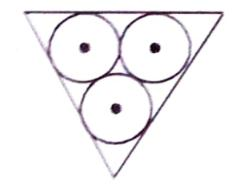
\includegraphics[width=2.5cm]{figs/figure.png}
    \label{fig:figure}
\end{figure}
\begin{enumerate}
\item $4+2\sqrt{3}$
\item $6+4\sqrt{3}$
\item $12+\frac{7\sqrt{3}}{4}$
\item $3+\frac{7\sqrt{3}}{4}$
\end{enumerate}
\hfill (2005S)

\item In a triangle $ABC$, $a, b, c$  are the lengths of its sides and $A, B, C$ are the angles of triangle $ABC$. The correct relation is given by
\begin{enumerate}
\item $\brak{b-c} \sin \brak{\frac{B-C}{2}} = a \cos \brak{\frac{A}{2}}$
\item $\brak{b-c} \cos \brak{\frac{A}{2}} = a \sin \brak{\frac{B-C}{2}}$
\item $\brak{b-c} \sin \brak{\frac{B+C}{2}} = a \cos \brak{\frac{A}{2}}$
\item $\brak{b-c} \cos \brak{\frac{A}{2}} = a \sin \brak{\frac{B+C}{2}}$
\end{enumerate}
\hfill (2005S)

\item One angle of an isosceles $\triangle$ is $120\degree$ and radius of its incircle $= \sqrt{3}$. Then the area of the triangle in sq. units is 
\begin{enumerate}
\item $7+12\sqrt{3}$
\item $12-7\sqrt{3}$
\item $12+7\sqrt{3}$
\item $4\pi$
\end{enumerate}
\hfill (2006 - 3M, -1)

\item Let $ABCD$ be a quadrilateral with area $18$, with side $AB$ parallel to the side $CD$ and $2AB = CD$. Let $AD$ be perpendicular to $AB$ and $CD$. If a circle is drawn inside the quadrilateral $ABCD$ touching all the sides, then the radius is
\begin{enumerate}
\item $3$
\item $2$
\item $\frac{3}{2}$
\item $1$
\end{enumerate}
\hfill (2007 - 3 Marks)

\item If the angles $A, B$ and $C$ of a triangle are in an arithmetic progression and if $\vec{a}, \vec{b}$ and $\vec{c}$ denote the lengths of the sides opposite to $A, B$ and $C$ respectively, then the value of the expression $\frac{a}{c}\sin 2C + \frac{c}{a} \sin 2A$ is
\begin{enumerate}
\item $\frac{1}{2}$
\item $\frac{\sqrt{3}}{2}$
\item $1$
\item $\sqrt{3}$
\end{enumerate}
\hfill (2010)

\item Let $PQR$ be a triangle of area $\Delta$ with $a=2, b= \frac{7}{2}$ and $c=\frac{5}{2}$, where $\vec{a}, \vec{b}$ and $\vec{c}$ are the lengths of the sides of the triangle opposite to the angles at $P, Q$ and $R$ respectively. Then $\frac{2\sin P - \sin 2P}{2\sin P + \sin 2P}$ equals
\begin{enumerate}
\item $\frac{3}{4\Delta}$
\item $\frac{45}{4\Delta}$
\item $\brak{\frac{3}{4\Delta}}^2$
\item $\brak{\frac{45}{4\Delta}}^2$
\end{enumerate}
\hfill (2012)

\item In a triangle the sum of two sides is $\vec{x}$ and the product of the same sides is $\vec{y}$. If $x^2-c^2=y$, where $\vec{c}$ is the third side of the triangle, then the ratio of the inradius to the circum-radius of the triangle is
\begin{enumerate}
\item $\frac{3y}{2\brak{x+c}}$
\item $\frac{3y}{2c\brak{x+c}}$
\item $\frac{3y}{4x\brak{x+c}}$
\item $\frac{3y}{4c\brak{x+c}}$
\end{enumerate}
\hfill (JEE Adv. 2014)

%\end{enumerate}


\end{enumerate}
\subsection*{Subjective Questions}
\begin{enumerate}[label=\thesubsection.\arabic*,ref=\thesubsection.\theenumi]

\iffalse
\title{Properties of Triangles}
\author{EE24Btech11022 - Eshan sharma}
\section{subjective}
\fi
%begin{document}
%begin{enumerate}
     \item A triangle $ABC$ has sides $AB=AC=5 cm$ and $BC =6 cm$. Triangle $A'B'C'$ is the reflection of the triangle $ABC$ in a line parallel to $AB$ placed at a distance of $2$ cm from $AB$, outside the triangle $ABC$. Triangle $A"B"C"$ is the reflection of the triangle $A'B'C'$ in a line parallel $B'C'$ placed at a distance of $2 cm$ from $B'C'$ outside the triangle $A'B'C'$. Find the distance between $\vec{A}$ and $\vec{A'}$.\hfill {(1978)}
     \item 
     \begin{enumerate}
     	\item If a circle is inscribed in a right angled triangle $ABC$ right angled at $\vec{B}$, show that the diameter of the circle is equal to $AB+BC-AC$.
     	\item If a triangle is inscribed in a circle, then the product of any two sides of the triangle is equal to the product of the diameter and perpendicular distance of the third side from the opposite vertex. Prove the above statement.
     \end{enumerate}
     \hfill {(1979)}
     \item
     \begin{enumerate}
     	\item A baloon is observed simultaneously from three points $\vec{A},\vec{B} \text{ and } \vec{C}$ on a straight road directly beneath it. The angular elevation at $\vec{B}$ is twice that at $\vec{A}$ and angular elevation at $\vec{C}$ is thrice that of $\vec{A}$. If the distance between $\vec{A}$ and $\vec{B}$ is $a$ and the distance between $\vec{B}$ and $\vec{C}$ is $b$, find height of baloon in terms of $a \text{ and } b$.
     	\item Find the area of the smaller part of a disc of radius $10 cm$, cut off by a chord $AB$ which subtends an angle of $22\frac{1}{2} \degree$ at the circumference.
     \end{enumerate}
     \hfill {(1980)}
     \item $ABC$ is a triangle. $\vec{D}$ is the middle point of $BC$. If $AD$ is perpendicular to $AC$, then prove that $\cos{A}\cos{C} = \frac{2(c^{2}-a^{2}}{3ac}$.
     \hfill {(1980)}
     \item $ABC$ is a triangle with $AB=AC$. $\vec{D}$ is any point on the side $BC$. $\vec{E}$ and $\vec{F}$ are points on the side $AB \text{ and } AC$, respectively, such that $DE$ is parallel to $AC, \text{ and } DF$ is parallel to $AB$. Prove that \\
     $DF + FA + AE + ED = AB+AC$
     \hfill {(1980)} 
%end{enumerate}
%end{document}

\iffalse
\title{13/A/E/6-21}
\author{EE24BTECH11040 - Mandara Hosur}
\section{subjective}
\fi

%\begin{enumerate}

\item 
\begin{enumerate}
\item $PQ$ is a vertical tower. $P$ is the foot and $Q$ is the top of the tower. $A$, $B$, $C$ are three points in the horizontal plane through P. The angles of elevation of $Q$ from $A$, $B$, $C$ are equal, and each is equal to $\theta$. The sides of the triangle $ABC$ are $a$, $b$, $c$; and the area of the triangle $ABC$ is $\Delta$. Show that the height of the tower is $\frac{abc\tan{\theta}}{4\Delta}$.
\item $AB$ is a vertical pole. The end $A$ is on the level ground. $C$ is the middle point of $AB$. $P$ is a point on the level ground. The portion $CB$ subtends an angle $\beta$ at $P$. If $AP=nAB$ then show that $\tan{\beta}=\frac{n}{2n^2+1}$.
\end{enumerate}

\hfill{\brak{1980}}

\item Let the angles $A$, $B$, $C$ of a triangle $ABC$ be in A.P. and let $b:c=\sqrt{3}:\sqrt{2}$. Find the angle $A$. 

\hfill{\brak{1981 - 2 Marks}}

\item A vertical pole stands at a point $Q$ on a horizontal ground. $A$ and $B$ are points on the ground, $d$ meters apart. The pole subtends angles $\alpha$ and $\beta$ at $A$ and $B$ respectively. $AB$ subtends an angle $\gamma$ at $Q$. Find the height of the pole. 

\hfill{\brak{1982 - 3 Marks}}

\item Four ships $A$, $B$, $C$ and $D$ are at sea in the following relative positions: $B$ is on the straight line segment $AC$, $B$ is due North of $D$ and $D$ is due west of $C$. The distance between $B$ and $D$ is 2 km. $\angle{BDA}=40\degree$, $\angle{BCD}=25\degree$. What is the distance between $A$ and $D$? $\sbrak{\text{Take} \sin{25\degree}=0.423}$

\hfill{\brak{1983 - 3 Marks}}

\item The ex-radii $r_1$, $r_2$, $r_3$ of $\Delta ABC$ are in H.P. Show that its sides $a$, $b$, $c$ are in A.P.

\hfill{\brak{1983 - 3 Marks}} 

\item For a triangle $ABC$ it is given that $\cos{A}+\cos{B}+\cos{C}=\frac{3}{2}$. Prove that the triangle is equilateral. 

\hfill{\brak{1984 - 4 Marks}}

\item With usual notation, if in a triangle $ABC$; $\frac{b+c}{11}=\frac{c+a}{12}=\frac{a+b}{13}$ then prove that $\frac{\cos{A}}{7}=\frac{\cos{B}}{19}=\frac{\cos{C}}{25}$. 

\hfill{\brak{1984 - 4 Marks}}

\item A ladder rests against a wall at an angle $\alpha$ to the horizontal. Its foot is pulled away from the wall through a distance $a$, so that it slides a distance $b$ down the wall making an angle $\beta$ with the horizontal. Show that $a=b\tan{\frac{1}{2}\brak{\alpha+\beta}}$.

\hfill{\brak{1985 - 5 Marks}}

\item In a triangle $ABC$, the median to the side $BC$ is of length $\frac{1}{\sqrt{11-6\sqrt{3}}}$ and it divides the angle $A$ into angles $30\degree$ and $45\degree$. Find the length of the side $BC$.

\hfill{\brak{1985 - 5 Marks}}

\item If in a triangle $ABC$, $\cos{A}\cos{B}+\sin{A}\sin{B}\sin{C}=1$, show that $a:b:c=1:1:\sqrt{2}$.

\hfill{\brak{1986 - 5 Marks}}

\item A sign-post in the form of an isosceles triangle $ABC$ is mounted on a pole of height $h$ fixed to the ground. The base $BC$ of the triangle is parallel to the ground. A man standing on the ground at a distance $d$ from the sign-post finds that the top vertex $A$ of the triangle subtends an angle $\beta$ and either of the other two vertices subtends the same angle $\alpha$ at his feet. Find the area of the triangle. 

\hfill{\brak{1988 - 5 Marks}}

\item $ABC$ is a triangular park with $AB=AC=100$m. A television tower stands at the midpoint of $BC$. The angles of elevation of the top of the tower at $A$, $B$, $C$ are $45\degree$, $60\degree$, $60\degree$, respectively. Find the height of the tower. 

\hfill{\brak{1989 - 5 Marks}}

\item A vertical tower $PQ$ stands at a point $P$. Points $A$ and $B$ are located to the South and East of $P$ respectively. $M$ is the mid point of $AB$. $PAM$ is an equilateral triangle; and $N$ is the foot of the perpendicular from $P$ on $AB$. Let $AN=20$ metres and the angle of elevation of the top of the tower at $N$ is $\tan^{-1}{2}$. Determine the height of the tower and the angles of elevation of the top of the tower at $A$ and $B$.

\hfill{\brak{1990 - 4 Marks}}

\item The sides of a triangle are three consecutive natural numbers and its largest angle is twice the smallest one. Determine the sides of the triangle.

\hfill{\brak{1991 - 4 Marks}}

\item In a triangle of base $a$ the ratio of the other two sides is $r\brak{<1}$. Show that the altitude of the triangle is less than or equal to $\frac{ar}{1-r^2}$.

\hfill{\brak{1991 - 4 Marks}}

\item A man notices two objects in a straight line due west. After walking a distance $c$ due north he observes that the objects subtend an angle $\alpha$ at his eye; and, after a further distance $2c$ due north, and angle $\beta$. Show that the distance between the objects is $\frac{8c}{3\cot{\beta}-\cot{\alpha}}$; the height of the man is being ignored. 

\hfill{\brak{1991 - 4 Marks}}

%\end{enumerate}

%\end{document}



\end{enumerate}
\fi

\subsection{Circle}
\begin{enumerate}[label=\thesubsection.\arabic*.,ref=\thesubsection.\theenumi]
\item  The perpendicular from the centre of a circle to a chord bisects the chord. 
\item  The line drawn through the centre of a circle to bisect a chord is perpendicular to the chord.
\item  There is one and only one circle passing through three non-collinear points. 
\item  Equal chords of a circle (or of congruent circles) are equidistant from the centre (or corresponding centres).
\item Chords equidistant from the centre (or corresponding centres) of a circle (or of congruent circles) are equal.
%
\item AB is a diameter of the circle, $CD$ is a chord equal to the radius of the circle. $AC$ and $BD$ when extended intersect at a point $E$. Prove that $\angle AEB = 60\degree$.
\item If the non-parallel sides of a trapezium are equal, prove that it is cyclic.
\item Prove that the line of centres of two intersecting circles subtends equal angles at the
two points of intersection.
\item  The angle subtended by an arc at the centre is double the angle subtended by it at any point on the remaining part of the circle.
\item Angles in the same segment of a circle are equal. \item  Angle in a semicircle is a right angle. 
\item  If a line segment joining two points subtends equal angles at two other points lying on the same side of the line containing the line segment, the four points lie on a circle. 
	\iffalse
\begin{enumerate}
\begin{figure}[!ht]
\centering
\resizebox{\columnwidth}{!}{	\begin{tikzpicture}
[scale=2,>=stealth,point/.style={draw,circle,fill = black,inner sep=0.5pt},]

%Triangle sides
\def\a{5}
\def\b{6}
\def\c{4}
\def\R{3.023715784073818}

%Coordinates of A
%\def\p{0.5}
\def\p{((\a^2+\c^2-\b^2)/(2*\a))}
\def\q{{sqrt(\c^2-\p^2)}}

\def\x{((\a^2+\b^2-\c^2)/(2*\a))}
\def\y{{sqrt(\b^2-\x^2)}}

%Labeling points
%\node (A) at ($({((\a^2+\c^2-\b^2)/(2*\a))},{sqrt(\c^2-\x^2)} )$)[point,label=above right:$A$] {};
\node (A) at ($({((\a^2+\c^2-\b^2)/(2*\a))},{sqrt(\c^2-\p^2)} )$)[point,label=below left:$A$] {};
\node (B) at (0, 0)[point,label=below left:$B$] {};
\node (C) at (\a, 0)[point,label=below right:$C$] {};
\node (D) at ($({((\a^2+\b^2-\c^2)/(2*\a))},{sqrt(\b^2-\x^2)} )$)[point,label=below left:$D$] {};
%\node (E) at ($({(\a)}, {((\a)/((\a^2+\b^2-\c^2)/(2*\a))*(sqrt(\c^2-\p^2))})$)[point,label=below right:$E$] {};
%Circumcentre

\node (O) at (2.5,1.70084013)[point,label=above right:$O$] {};

%Drawing triangle ABC
\draw (A) -- node[left] {$\textrm{c}$} (B) -- node[below] {$\textrm{a}$} (C) -- node[above,yshift=2mm] {$\textrm{b}$} (A);

\draw (D) -- node[left] {$\textrm{e}$} (B);
\draw (D) -- node[left] {$\textrm{d}$} (C);

%\draw[dashed] (E) -- node[left] {$\textrm{}$} (B);
%\draw[dashed] (E) -- node[left] {$\textrm{}$} (C);
%Drawing OA, OB, OC
%\draw (O) -- node[left] {$\textrm{R}$} (A);
%\draw (O) -- node[below] {$\textrm{R}$} (B);
%\draw (O) -- node[below] {$\textrm{R}$} (C);
\draw (O) circle (\R);

%\tkzMarkAngle[fill=blue!50,size=.3](C,B,A)
%\tkzMarkAngle[fill=blue!50,size=.3](O,C,B)


%\tkzMarkAngle[fill=red!50](O,A,C)
\tkzMarkAngle[fill=red!50,size=.3](B,D,C)
%\tkzMarkAngle[fill=red!50,size=.3](B,E,C)

\tkzMarkAngle[fill=orange!50,size=.3](B,A,C)
%\tkzMarkAngle[fill=orange!50,size=.3](O,B,A)
\tkzMarkAngle[fill=red!50,size=.3](B,D,C)
\tkzMarkAngle[fill=red!50,size=.3](C,B,D)
\tkzMarkAngle[fill=red!50,size=.3](D,C,B)
%\tkzLabelAngle[pos=0.5](A,C,B){$\theta_1$}
%\tkzLabelAngle[pos=0.5](O,B,C){$\theta_1$}
\tkzLabelAngle[pos=0.5](B,D,C){$\theta_2$}
%\tkzLabelAngle[pos=0.5](B,E,C){$\theta_3$}

\tkzLabelAngle[pos=0.5](B,A,C){$\theta_1$}
%\tkzLabelAngle[pos=1.5](O,C,A){$\theta_3$}
\tkzLabelAngle[pos=0.5](C,B,D){$\beta_2$}
\tkzLabelAngle[pos=0.5](D,C,B){$\alpha_2$}

	
	\end{tikzpicture}
	}
\caption{ }
\label{fig:8.5.13_C_circle}	
\end{figure}
%
\item {\em Construction: }See Fig. \ref{fig:8.5.13_C_circle}.  The input parameters are
% 
\begin{align}
\vec{A} &= \myvec{p \\ q}
\\
\vec{B} &= \myvec{0 \\ 0}
\\
\vec{C} &= \myvec{a\\ 0} 
\end{align}
\subitem $\theta_1$ is obtained using
%
\begin{align}
\cos{\theta_1} = \frac{\brak{\vec{A}-\vec{B}}^T\brak{\vec{A}-\vec{C}}}{\norm{\vec{A}-\vec{B}}\norm{\vec{A}-\vec{C}}}
\end{align}
\subitem Let 
\begin{align}
\vec{D} &= b\myvec{\cos \beta_2\\ b \sin \beta_2} 
\label{eq:8.5.13_D}
\end{align}
From the given information, $\theta_2 = \theta_1$
\begin{align}
\implies \frac{b}{\sin\brak{\theta_2 + \beta_2}} = \frac{a}{\sin \theta_2}
\label{eq:8.5.13_b}
\end{align}
%
Choosing an appropriate value of $\beta_2$, $b$ and $\vec{D}$ can be obtained from \eqref{eq:8.5.13_D} and \eqref{eq:8.5.13_b} respectively.
\subitem The circumcircle of $\triangle ABC$ can then be drawn and it can be verified that $\vec{D}$ lies on it.

\item {Proof: } Let 
\begin{align}
\vec{O} = \myvec{0\\0}
\end{align}
%
be the circumcentre of $\triangle ABC$ and let $r$ be the radius.  Assuming that
\begin{align}
\label{eq:8.5.13_A}
\vec{A} &= r\myvec{\cos \theta_1\\\sin\theta_1},
\vec{B} = r\myvec{\cos \theta_2\\\sin\theta_2}
\\
\vec{C} &= r\myvec{\cos \theta_3\\\sin\theta_3},
\vec{D} = k\myvec{\cos \theta_4\\\sin\theta_4}
\label{eq:8.5.13_Dp}
\end{align}
in Fig. \ref{fig:8.5.13_C_circle}, from the given information
\begin{align}
 \frac{\brak{\vec{A}-\vec{B}}^T\brak{\vec{A}-\vec{C}}}{\norm{\vec{A}-\vec{B}}\norm{\vec{A}-\vec{C}}} = 
 \frac{\brak{\vec{D}-\vec{B}}^T\brak{\vec{D}-\vec{C}}}{\norm{\vec{D}-\vec{B}}\norm{\vec{D}-\vec{C}}} 
\label{eq:8.5.13_inner}
\end{align}
\begin{multline}
\because \brak{\vec{A}-\vec{B}}^T\brak{\vec{A}-\vec{C}} = \norm{\vec{A}}^2 - \vec{A}^T\vec{B}
\\
- \vec{B}^T\vec{A}+ \vec{B}^T\vec{C}
\label{eq:8.5.13_inner_expand}
\end{multline}
from \eqref{eq:8.5.13_A}-\eqref{eq:8.5.13_Dp}, \eqref{eq:8.5.13_inner_expand} can be expressed as
\begin{multline}
r^2\lsbrak{1 - \cos \brak{\theta_1-\theta_2} }
\\
\rsbrak{-  \cos \brak{\theta_1-\theta_3}+ \cos \brak{\theta_2-\theta_3}}
\\
=  r^2\brak{1-p_{12}- p_{13}+ p_{23}}
\label{eq:8.5.13_abc_inner}
\end{multline}
which can be expressed as
\begin{multline}
2r^2\lsbrak{ \sin^2 \brak{\frac{\theta_1-\theta_2}{2}} }
\\
+
\rsbrak{  \sin \brak{\frac{\theta_1-\theta_2}{2}}\sin \brak{\frac{\theta_1+\theta_2}{2} - \theta_3}}
\\
= 2r^2 \sin \brak{\frac{\theta_1-\theta_2}{2}} 
\\
\times
\sbrak{\sin \brak{\frac{\theta_1-\theta_2}{2}}
 + \sin \brak{\frac{\theta_1+\theta_2}{2} - \theta_3}}
\\
= 4r^2 \sin \brak{\frac{\theta_1-\theta_2}{2}} 
\\
\times \sin \brak{\frac{\theta_1-\theta_3}{2}} \cos \brak{\frac{\theta_2-\theta_3}{2}}
\label{eq:8.5.13_abc_innercos}
\end{multline}
%
Similarly, 
\begin{multline}
 \brak{\vec{D}-\vec{B}}^T\brak{\vec{D}-\vec{C}} = \norm{\vec{D}}^2 - \vec{D}^T\vec{B}
\\
- \vec{B}^T\vec{D}+ \vec{B}^T\vec{C}
\end{multline}
which can be expressed using \eqref{eq:8.5.13_A}-\eqref{eq:8.5.13_Dp} as
\begin{multline}
 k^2 -rk \cos\brak{\theta_2-\theta_4}
\\
-rk \cos\brak{\theta_3-\theta_4}+r^2 \cos\brak{\theta_2-\theta_3}
\\
=  k^2 -rk p_{24}-rk p_{34}+r^2  p_{23}
\label{eq:8.5.13_inner_dexpand}
\end{multline}
%
Similarly, 
\begin{align}
\norm{\vec{A}-\vec{B}}^2 &= 2r^2\sbrak{1 -  \cos \brak{\theta_1-\theta_2} } 
\\
&= 2r^2\brak{1 - p_{12}}
\label{eq:8.5.13_inner_normab}
\\
&=2 \sin^2 \brak{\frac{\theta_1-\theta_2}{2}} 
\label{eq:8.5.13_inner_normabcos}
\\
\norm{\vec{A}-\vec{C}}^2 &= 2r^2\sbrak{1 -  \cos \brak{\theta_1-\theta_3} } 
\\
&= 2r^2\brak{1 - p_{13}}
\label{eq:8.5.13_inner_normac}
\\
&=2 \sin^2 \brak{\frac{\theta_1-\theta_3}{2}} 
\label{eq:8.5.13_inner_normaccos}
\\
\norm{\vec{D}-\vec{B}}^2 &= k^2 + r^2 - 2kr \cos\brak{\theta_2-\theta_4} 
\\
&= k^2+r^2 - 2kr p_{24}
\label{eq:8.5.13_inner_normdb}
\\
\norm{\vec{D}-\vec{C}}^2 &= k^2 + r^2 - 2kr \cos\brak{\theta_3-\theta_4} 
\\
&= k^2+r^2 - 2kr p_{34}
\label{eq:8.5.13_inner_normdc}
\end{align}
%
Substituting from \eqref{eq:8.5.13_inner_dexpand}, \eqref{eq:8.5.13_abc_inner},
\eqref{eq:8.5.13_inner_normab},
\eqref{eq:8.5.13_inner_normac},
\eqref{eq:8.5.13_inner_normdb},
\eqref{eq:8.5.13_inner_normdc}
 in \eqref{eq:8.5.13_inner}, 
\begin{multline}
\frac{r^2\brak{1-p_{12}- p_{13}+ p_{23}}}{\sqrt{2r^2\brak{1 - p_{12}}}\sqrt{2r^2\brak{1 - p_{13}}}} 
\\
= \frac{k^2 -rk p_{24}-rk p_{34}+r^2  p_{23}}{\sqrt{k^2+r^2 - 2kr p_{24}}\sqrt{k^2+r^2 - 2kr p_{34}}}
\end{multline}
which can be expressed as 
\begin{multline}
\frac{1-p_{12}- p_{13}+ p_{23}}{2\sqrt{\brak{1 - p_{12}}\brak{1 - p_{13}}}}
\\
= \frac{x^2 -x p_{24}-x p_{34}+  p_{23}}{\sqrt{\brak{x^2+1 - 2x p_{24}}\brak{x^2+1 - 2x p_{34}}}}
\label{eq:8.5.13_inner_x}
\end{multline}
upon substituting
\begin{align}
x =\frac{k}{r}.
\label{eq:8.5.13_xkr}
\end{align}
From \eqref{eq:8.5.13_abc_innercos}, \eqref{eq:8.5.13_inner_normabcos}
and \eqref{eq:8.5.13_inner_normaccos},
\begin{multline}
\frac{1-p_{12}- p_{13}+ p_{23}}{2\sqrt{\brak{1 - p_{12}}\brak{1 - p_{13}}}} 
\\
= \cos \brak{\frac{\theta_2-\theta_3}{2}}
\label{eq:8.5.13_inner_123}
\end{multline}
Similarly, it can be shown that
\begin{multline}
\frac{1-p_{24}- p_{34}+ p_{23}}{2\sqrt{\brak{1 - p_{24}}\brak{1 - p_{34}}}} 
\\
= \cos \brak{\frac{\theta_2-\theta_3}{2}}
\label{eq:8.5.13_inner_234}
\end{multline}
From \eqref{eq:8.5.13_inner_123} and \eqref{eq:8.5.13_inner_234}, \eqref{eq:8.5.13_inner_x}
can be expressed as
\begin{multline}
\frac{1-p_{24}- p_{34}+ p_{23}}{2\sqrt{\brak{1 - p_{24}}\brak{1 - p_{34}}}} 
\\
= \frac{x^2 -x p_{24}-x p_{34}+  p_{23}}{\sqrt{\brak{x^2+1 - 2x p_{24}}\brak{x^2+1 - 2x p_{34}}}}
\label{eq:8.5.13_inner_x23}
\end{multline}
It is obvious that 
\begin{align}
x = 1
\end{align}
%
is a solution of \eqref{eq:8.5.13_inner_x23}
\begin{align}
\implies k = r
\end{align}
from \eqref{eq:8.5.13_xkr}.


\end{enumerate}
\fi
\item  The sum of either pair of opposite angles of a cyclic quadrilateral is 180$\degree$.
\item  If sum of a pair of opposite angles of a quadrilateral is 180$\degree$, the quadrilateral is cyclic.
%
\item AB is a diameter of the circle, $CD$ is a chord equal to the radius of the circle. $AC$ and $BD$ when extended intersect at a point $E$. Prove that $\angle AEB = 60\degree$.
\item Two circles of radii 5 cm and 3 cm intersect at two points and the distance between their centres is 4 cm. Find the length of the common chord.
\item Two chords $AB$ and $CD$ of lengths 5 cm and 11 cm respectively of a circle are parallel
to each other and are on opposite sides of its centre. If the distance between $AB$ and
$CD$ is 6 cm, find the radius of the circle.
\item The lengths of two parallel chords of a circle are 6 cm and 8 cm. If the smaller chord is
at distance 4 cm from the centre, what is the distance of the other chord from the
centre?
\item  Two concentric circles are of radii 5 cm and 3 cm. Find the length of the chord of the larger circle which touches the smaller circle.
\item A $\triangle ABC$ is drawn to circumscribe a circle of radius 4 cm such that the segments $BD$ and $DC$ into which $BC$ is divided by the point of contact $D$ are of lengths 8 cm and 6 cm respectively. Find the sides $AB$ and $AC$.
\item $PQ$ is a chord of length 8 cm of a circle of radius 5 cm. The tangents at $P$ and $Q$ intersect at a point $T$. Find the length $TP$.
\item Two circles intersect at two points $A and B$. $AD$ and $AC$ are diameters to the two circles. Prove that $B$ lies on the line segment $DC$.
\item Prove that the quadrilateral formed (if possible) by the internal angle bisectors of any quadrilateral is cyclic.
\item  The perpendicular from the centre of a circle to a chord bisects the chord. 
\item  The line drawn through the centre of a circle to bisect a chord is perpendicular to the chord.
\item  There is one and only one circle passing through three non-collinear points. 
\item  Equal chords of a circle (or of congruent circles) are equidistant from the centre (or corresponding centres).
\item If a line intersects two concentric circles (circles with the same centre) with centre O at A, B, C and D, prove that AB = CD.
	\iffalse
\begin{enumerate}
\begin{figure}[!ht]
\centering
\resizebox{\columnwidth}{!}{\begin{tikzpicture}[scale = 0.5,>=stealth,point/.style={draw,circle,fill=black, inner sep=0.5pt},]
\node (O) at (0, 0)[point,label=above:$O$] {};
\node (A) at (-8.66, -5)[point,label=below:$A$] {};
\node (B) at (-4.89, -5)[point,label=below:$B$] {};
\node (C) at (4.89, -5)[point,label=below:$C$] {};
\node (D) at (8.66, -5)[point,label=below:$D$] {};
\node (M) at (0,-5)[point,label=below:$M$] {};

\draw (0,0) circle(7cm);
\draw (0,0) circle(10cm);
\draw (A) -- node[below=5pt]{}(B) -- (C) -- (D);
\draw[dotted] (O) -- node[below=5pt]{}(M);
\draw[dotted] (O) -- node[below=5pt]{}(A);
\draw[dotted] (O) -- node[below=5pt]{}(B);
\draw[dotted] (O) -- node[below=5pt]{}(C);
\draw[dotted] (O) -- node[below=5pt]{}(D);

\tkzMarkRightAngle[fill=blue!20, mark=|](O,M,B)

\end{tikzpicture}}
\caption{}
\label{fig:8.5.40_circle_1}	
\end{figure}

\item  {\em Construction: } See Fig. \ref{fig:8.5.40_circle_1}.	 The input parameters are
\begin{align}
\vec{O} &= \myvec{0\\0},
\vec{A} &= r_1\myvec{\cos \theta_1\\ \sin \theta_1}
\vec{D} &= r_2\myvec{\cos \theta_2\\ \sin \theta_2}
\end{align}
The two concentric circles  with centre $\vec{O}$ and radii $r_1$ and $r_2$ are drawn.

\subitem The equation of $AD$ is 
\begin{align}
\label{eq:8.1.40_line}
\vec{x} = \vec{A} + \lambda \brak{\vec{A}-\vec{D}}
\end{align}
Points $\vec{B}$ and $\vec{D}$ are obtained as the intersection of $AB$ and the circle with equation
\begin{align}
\label{eq:8.1.40_circle}
\norm{\vec{x}}^2 = r_2^2
\end{align}
From \eqref{eq:8.1.40_circle}
and \eqref{eq:8.1.40_circle}, 
\begin{align}
\norm{\vec{A} + \lambda \brak{\vec{A}-\vec{D}}}^2 = r_2^2
\end{align}
\begin{multline}
\lambda^2\norm{\vec{A}-\vec{D}}^2 + 2\lambda \vec{A}^T\brak{\vec{A}-\vec{D}} 
\\
+ \norm{\vec{A}}^2 -r_2^2 =0
\label{eq:8.1.40_quad}
\end{multline}
Solving the above quadratic equation yields two values for $\lambda$ yielding $\vec{B}$ and $\vec{C}$.  
\begin{align}
\vec{M} = \frac{\vec{B}+\vec{C}}{2}
\end{align}


\item {\em Proof: } In Fig. \ref{fig:8.5.40_circle_1}, 
\begin{align}
\triangle OMB \cong \triangle OMC
\\
\triangle OMA \cong \triangle OMD
\end{align}
resulting in 
\begin{align}
AM = DM
\\
BM = CM
\\
\implies AB = CD
\end{align}

\end{enumerate}
\fi
\item A chord of a circle is equal to the radius of the
circle. Find the angle subtended by the chord at
a point on the minor arc and also at a point on the
major arc.
\item If diagonals of a cyclic quadrilateral are diameters of the circle through the vertices of
the quadrilateral, prove that it is a rectangle.
\item If the non-parallel sides of a trapezium are equal, prove that it is cyclic.
	\iffalse
\begin{enumerate}

\begin{figure}[!ht]
\centering
\resizebox{\columnwidth}{!}{\begin{tikzpicture}[scale=1.5,>=stealth,point/.style={draw,circle,fill = black,inner sep=0.5pt},]
      
%Labeling points
\node (A) at (0, 0)[point,label=below left:$A$] {};
\node (B) at (5, 0)[point,label=below right:$B$] {};
\node (C) at (3.9, 3)[point,label=above right:$C$] {};
\node (D) at (1.1, 3)[point,label=above left:$D$] {};
\node (P1) at (1.1, 0)[point,label=below right:$P_1$] {};
\node (P2) at (3.9, 0)[point,label=below left:$P_2$] {};
\node (O) at (2.5, 0.79)[point,label=below:$O$]{};

%Drawing quad ABCD
\draw (A) -- node[below=6pt]{$b$}(B) -- (C) -- (D) -- (A);
\draw[dotted] (D) -- node[right = 7pt]{$h$}(P1)(P2)--(C);
\draw[dotted] (O) circle(2.62);
%marking line segment
\tkzMarkSegments[mark=|,size=6pt](A,D C,B)
\tkzMarkSegments[mark=s||,size=6pt](P1,D C,P2)

%marking angles
\tkzMarkAngle[fill=orange!40,size=0.5cm,mark=](P1,A,D)
\tkzMarkAngle[fill=orange!40,size=0.5cm,mark=](D,C,B)
\tkzMarkRightAngle[fill=blue!20](D,P1,A)
\tkzMarkRightAngle[fill=blue!20](C,P2,B)
\tkzLabelAngle[pos=0.75](P1,A,D){$\theta$}
\tkzLabelAngle[pos=0.75](D,C,B){$\alpha$}

\end{tikzpicture} }
\caption{}
\label{fig:8.5.43_trapezium}	
\end{figure}
%
\item {\em Construction: }See Fig. \ref{fig:8.5.43_trapezium}
The input parameters are
\begin{align}
\vec{A} &=\myvec{0\\0},
\vec{B} &= \myvec{b\\0}, \label{eq:8.5.43_constr_b}
\\
\vec{C} &= \myvec{b - h\cot{\theta}\\h}\label{eq:8.5.43_constr_c}\\ 
\vec{D} &= h\myvec{\cot{\theta}\\ 1}\label{eq:8.5.43_constr_d}	\end{align}
%
which are sufficient to draw the trapezium.  The circumcircle of $\triangle ABC$ is then drawn.  This circle passes through $\vec{D}$.

From \eqref{eq:8.5.43_constr_b} - \eqref{eq:8.5.43_constr_d}
\begin{align}
\vec{B} - \vec{A} &= \myvec{b\\0}\label{eq:8.5.43_dir1}\\
\vec{D} - \vec{C} &= \myvec{2h\cot{\theta}-b\\0}\label{eq:8.5.43_dir2}\\
\vec{D} - \vec{A} &= \myvec{h\cot{\theta}\\h}\label{eq:8.5.43_dir3}\\
\vec{B} - \vec{C} &= \myvec{h\cot{\theta}\\-h}\label{eq:8.5.43_dir4}
\end{align}

Finding the scalar products:
\begin{align}
\brak{\vec{D} - \vec{A}}^T\brak{\vec{B} - \vec{A}} &= \norm{\vec{D}-\vec{A}} 
\norm{ \vec{B}-\vec{A}} \cos{\theta}\label{eq:8.5.43_scalar1}\\
\brak{\vec{D} - \vec{C}}^T\brak{\vec{B} - \vec{C}} &= \norm{\vec{D}-\vec{C}} 
\norm{ \vec{B}-\vec{C}} \cos{\alpha}\label{eq:8.5.43_scalar2}
\end{align}

Dividing \eqref{eq:8.5.43_scalar2} with \eqref{eq:8.5.43_scalar1},
\begin{align}
\frac{\brak{\vec{D} - \vec{A}}^T\brak{\vec{B} - \vec{A}}}{\brak{\vec{D} - \vec{C}}^T\brak{\vec{B} - \vec{C}}} &= \frac{\norm{\vec{D}-\vec{A}}\ 
\norm{ \vec{B}-\vec{A}} \cos{\theta}}{\norm{\vec{D}-\vec{C}} 
\norm{ \vec{B}-\vec{C}} \cos{\alpha}}\label{eq:8.5.43_scalar3}
\end{align}\\
$\because \norm{ \vec{D} - \vec{A} } = \norm{ \vec{B} - \vec{C}} $, \eqref{eq:8.5.43_scalar3} can be simplified to the form
\begin{align}
\frac{\brak{\vec{D} - \vec{A}}^T\brak{\vec{B} - \vec{A}}}{\brak{\vec{D} - \vec{C}}^T\brak{\vec{B} - \vec{C}}} &= \frac{\norm{ \vec{B}-\vec{A}} \cos{\theta}}{\norm{\vec{D}-\vec{C}}cos{\alpha}}
\end{align}
%
Substituting values from \eqref{eq:8.5.43_dir1}, \eqref{eq:8.5.43_dir2}, \eqref{eq:8.5.43_dir3} and \eqref{eq:8.5.43_dir4}:
\begin{align}
\frac{bh\cot{\theta}}{\brak{2h\cot{\theta}-b}h\cot{\theta}} &= \frac{b\cos{\theta}}{b-2h\cot{\theta}}\\
\implies\cos{\alpha} &= -\cos{\theta}\\
\implies \alpha + \theta &= 180\degree
\end{align}

$\therefore ABCD$ is a cyclic quadilateral.

\end{enumerate}
\fi

\item Two circles intersect at two points $B$ and $C$.
Through $B$, two line segments $ABD$ and $PBQ$
are drawn to intersect the circles at $A, D$ and $P$,
$Q$ respectively. Prove that
$\angle ACP = \angle QCD$.
\item If circles are drawn taking two sides of a triangle as diameters, prove that the point of
intersection of these circles lie on the third side.
\item Prove that the line of centres of two intersecting circles subtends equal angles at the
two points of intersection.
\item Let the vertex of an angle $ABC$ be located outside a circle and let the sides of the angle
intersect equal chords $AD$ and $CE$ with the circle. Prove that $\angle ABC$ is equal to half the
difference of the angles subtended by the chords $AC$ and $DE$ at the centre.
\item Prove that the circle drawn with any side of a rhombus as diameter, passes through
the point of intersection of its diagonals.
\item $ABCD$ is a parallelogram. The circle through $A, B$ and $C$ intersect $CD$ (produced if
necessary) at $E$. Prove that $AE = AD$.
\item $AC$ and $BD$ are chords of a circle which bisect each other. Prove that (i) $AC$ and $BD$ are
diameters, (ii) $ABCD$ is a rectangle.
\item Bisectors of angles $A, B$ and $C$ of a $\triangle ABC$ intersect its circumcircle at $D, E$ and
$F$ respectively. Prove that the angles of the $\triangle DEF$ are $90\degree – \frac{A}{2}, 90\degree – \frac{B}{2}$ and $90\degree – \frac{C}{2}$.
\item Two congruent circles intersect each other at points A and B. Through A any line segment PAQ is drawn so that $P, Q$ lie on the two circles. Prove that $BP = BQ$.
\item In any $\triangle ABC$, if the angle bisector of $\angle A$ and perpendicular bisector of $BC$ intersect, prove that they intersect on the circumcircle of the $\triangle ABC$.
%
%
\item Prove that in two concentric circles, the chord of the larger circle, which touches the smaller circle, is bisected at the point of contact.
%
%
%
\end{enumerate}

\subsection{Olympiad}
\begin{enumerate}
\item $AB$ is tangent to the circles $CAMN$ and $NMBD$. $M$ lies between $C$ and $D$ on the line $CD$, and $CD$ is parallel to $AB$. The chords $NA$ and $CM$ meet at $P$; the chords $NB$ and $MD$ meet at $Q$. The rays $CA$ and $DB$ meet at $E$. Prove that $PE = QE$.\hfill(IMO 2000)
    \item Let $ABCD$ be a convex quadrilateral with perpendicular diagonals. If $AB = 20$, $BC = 70$, and $CD = 90$, then what is the value of $DA$?\hfill(PRERMO 2014)
    \item In a triangle with integer side lengths, one side is three times as long as a second side, and the length of the third side is $17$. What is the greatest possible perimeter of the triangle?\hfill(PRERMO 2014)
    \item In a triangle $ABC$, $X$ and $Y$ are points on the segments $AB$ and $AC$, respectively, such that $ AX : XB = 1 : 2 $ and $ AY : YC = 2 : 1.$If the area of triangle $AXY$ is $10$, then what is the area of triangle $ABC$?\hfill(PRERMO 2014)
    \item Let $XOY$ be a triangle with $\angle XOY = 90\degree$. Let $M$ and $N$ be the midpoints of legs $OX$ and $OY$, respectively. Suppose that $XN = 19$ and $YM = 22$. What is $XY$?\hfill(PRERMO 2014)
\item $PS$ is a line segment of length 4 and $O$ is the midpoint of $PS$. A semicircular arc is drawn with $PS$ as diameter. Let $X$ be the midpoint of this arc. $Q$ and $R$ are points on the arc $PXS$ such that $QR$ is parallel to $PS$ and the semicircular arc drawn with $QR$ as diameter is tangent to $PS$. What is the area of the region $QXROQ$ bounded by the two semicircular arcs?\hfill(PRERMO 2012)
\item $O$ and $I$ are the circumcentre and incentre of $\triangle ABC$ respectively. Suppose $O$ lies in the interior of $\triangle ABC$ and $I$ lies on the circle passing through $B$, $O$, and $C$. What is the magnitude of $\angle BAC$ in degrees?\hfill(PRERMO 2012)
\item In $\triangle ABC$, we have $AC = BC = 7$ and $AB = 2$. Suppose that $D$ is a point on line $AB$ such that $B$ lies between $A$ and $D$ and $CD = 8$. What is the length of the segment $BD$?\hfill(PRERMO 2012)
\item In rectangle $ABCD$, $AB = 5$ and $BC = 3$. Points $F$ and $G$ are on line segment $CD$ so that $DF = 1$ and $GC = 2$. Lines $AF$ and $BG$ intersect at $E$. What is the area of $\triangle ABE$?\hfill(PRERMO 2012)
\item A triangle with perimeter 7 has integer side lengths. What is the maximum possible area of such a triangle?\hfill(PRERMO 2012)
\item $ABCD$ is a square and $AB$ = 1 Equilateral triangles $AYB$ and $CXD$ are drawn such that $X$ and $Y$ are inside the square.What is the length of $XY$?\hfill(PRERMO 2012)
\item The figure below shows a broken piece of a circular plate made of glass.
    
	  
		\begin{figure}[h!]
    \centering
	    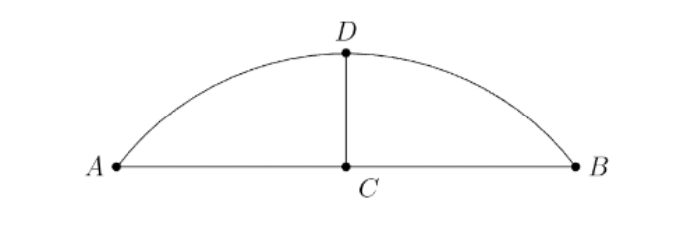
\includegraphics[width=\columnwidth]{olympiad/figs/permo.jpg}
    \end{figure}



    $ C $ is the midpoint of $ AB $, and $ D $ is the midpoint of arc $ AB $. Given that $ AB = 24 $ cm and $ CD = 6 $ cm, what is the radius of the plate in centimeters? (The figure is not drawn to scale.)\hfill(PRERMO 2015)

    \item A $ 2 \times 3 $ rectangle and a $ 3 \times 4 $ rectangle are contained within a square without overlapping at any interior point, and the sides of the square are parallel to the sides of the two given rectangles. What is the smallest possible area of the square? \hfill(PRERMO 2015)

    \item What is the greatest possible perimeter of a right-angled triangle with integer side lengths if one of the sides has length 12? \hfill(PRERMO 2015)

    \item In rectangle $ ABCD $, $ AB = 8 $ and $ BC = 20 $. Let $ P $ be a point on $ AD $ such that $ \angle BPC = 90\degree $. If $ r_1, r_2, r_3 $ are the radii of the incircles of triangles $ APB, BPC $, and $ CPD $, what is the value of $ r_1 + r_2 + r_3 $? \hfill(PRERMO 2015)


\item In the acute-angled triangle $ABC$, let $D$ be the foot of the altitude from $A$, and $E$ be the midpoint of $BC$. Let $F$ be the midpoint of $AC$. Suppose $ \angle BAE = 40\degree $. If $ \angle DAE = \angle DFE $, what is the magnitude of $ \angle ADF $ in degrees?\hfill(PRERMO 2015)

\item The circle $ \omega $ touches the circle $ \Omega $ internally at $ P $. The center $ O $ of $ \Omega $ is outside $ \omega $. Let $XY$ be a diameter of $ \Omega $ which is also tangent to $ \omega $. Assume $ PY > PX $. Let $ PY $ intersect $ \omega $ at $ Z $. If $ YZ = 2PZ $, what is the magnitude of $ \angle LPYX $ in degrees? \hfill(PRERMO 2015)
	\item On each side of an equilateral triangle with side length $n$ units, where $n$ is an integer,$1 \leq n \leq 100$ , consider $n - 1$ points that divide the side into $n$ equal segments.Through these points, draw lines parallel to the sides of the triangle, obtaining a net of equilateral triangles of side length one unit. On each of the vertices of these small triangles, place a coin head up. Two coins are said to be adjacent if the distance between them is $1$ unit. A move consists of flipping over any three mutually adjacent coins. Find the number of values of $n$ for which it is possible to turn all coins tail up after a finite number of moves.\hfill(IOQM 2015)


	\item In an equilateral triangle of side length $6$, pegs are placed at the vertices and also evenly along each side at a distance of $1$ from each other. Four distinct pegs are chosen from the $15$ interior pegs on the sides (that is, the chosen ones are not vertices of the triangle) and each peg is joined to the respective opposite vertex by a line segment.If $N$ denotes the number of ways we can choose the pegs such that the drawn linesegments divide the interior of the triangle into exactly nine regions, find the sum ofthe squares of the digits of $N$.\hfill(IOQM 2015)		
	\item In a triangle $ABC$, let $E$ be the midpoint of $AC$ and $F$ be the midpoint of $AB$. The medians $BE$ and $CF$ intersect at $G$. Let $Y$ and $Z$ be the midpoints of $BE$ and $CF$, respectively. If the area of triangle $ABC$ is 480, find the area of triangle $GYZ$.\hfill(IOQM 2015)
	    \item The six sides of a convex hexagon $A_{1}A_{2}A_{3}A_{4}A_{5}A_{6}$ are colored red. Each of the diagonals of the hexagon is colored either red or blue. If $N$ is the number of colorings such that every triangle $A_{i}A_{j}A_{k}$ , where $1 \leq i < j < k \leq 6$ , has at least one redside, find the sum of the squares of the digits of $N$ .\hfill(IOQM 2015)
    \item Let $X$ be the set of all even positive integers $n$ such that the measure of the angle of some regular polygon is $n$ degrees. Find the number of elements in $X$ .\hfill(IOQM 2015)
    
    \item Let $ABCD$ be a unit square. Suppose $M$ and $N$ are points on $BC$ and $CD$, respectively, such that the perimeter of triangle $MCN$ is $2$. Let $O$ be the circumcenter of triangle $MAN$, and $P$ be the circumcenter of triangle $MON$. If $\left(\frac{OP}{OA}\right)^2 = \frac{m}{n}$ for some relatively prime positive integers $m$ and $n$, find the value of $m + n$.\hfill(IOQM 2015)
    
    \item Let $ABC$ be a triangle in the $xy$-plane, where $B$ is at the origin $\brak{0, 0}$. Let $BC$ be produced to $D$ such that $BC : CD = 1 : 1$, $CA$ be produced to $E$ such that $CA : AE = 1 : 2$, and $AB$ be produced to $F$ such that $AB : BF = 1 : 3$. Let $G\brak{32, 24}$ be the centroid of triangle $ABC$ and $K$ be the centroid of triangle $DEF$. Find the length $GK$.\hfill(IOQM 2015)
    
    \item In the coordinate plane, a point is called a lattice point if both of its coordinates are integers. Let $A$ be the point $\brak{12, 84}$. Find the number of right-angled triangles $ABC$ in the coordinate plane where $B$ and $C$ are lattice points, having a right angle at the vertex $A$ and whose incenter is at the origin $\brak{0, 0}$.\hfill(IOQM 2015)
    
    \item A trapezium in the plane is a quadrilateral in which a pair of opposite sides are parallel. A trapezium is said to be non-degenerate if it has positive area. Find the number of mutually non-congruent, non-degenerate trapeziums whose sides are four distinct integers from the set $\cbrak{5, 6, 7, 8, 9, 10}$.\hfill(IOQM 2015)
    
    \item In triangle  $ABC$, point $ A_1 $ lies on side $ BC $ and point $B_1$ lies on side $ AC $. Let  $P$ and $ Q $ be points on segments 
$AA_1$ and $BB_1 $, respectively, such that   $PQ \parallel AB$.

Let
 $P_1$ be a point on line  $PB_1$ such that $B_1$ lies strictly between 
$P$ and $P_1$, and $\angle PP_1C$ = $\angle BAC$. Similarly, let $Q_1$ 
be a point on line $QA_1$ such that $A_1$ lies strictly between $Q$ and 
$Q_1$, and $ \angle CQ_1Q$ = $\angle CBA $.
Prove that points $P, Q, P_1,$ and $Q_1$ are concyclic.
\hfill(IMO 2019)


\item
 Let $I$ be the in center of acute triangle $ABC$ with $AB$ $\neq AC$. 
The incircle $\omega$ of $ABC$ is tangent to sides $ BC$, $CA$, and $AB$
 at points $D$,  $E$, and $F$, respectively. 


The line 
through $D$ perpendicular to $EF$ meets $\omega$ again at $R$. Line $AR$
 meets $omega$ again at $P$. The circumcircles of triangles $PCE$ and 
$PBF$ meet again at $Q$.

Prove that lines $DI$ and $PQ$ meet on the line through $ A$ that is perpendicular to $AI$.
\hfill(IMO 2019)
\item consider the convex quadrilateral ABCD.The point P is the interior of ABCD.The following ratio equalities hold:
\begin{align}
\angle PAD: \angle PBA: \angle DPA =1:2:3 = \angle CBP: \angle BAP: \angle BPC.
\end{align} 
prove
 that the following three lines meet in a point:the internal bisectors 
of angles $\angle ADP$ and $\angle PCB$ and the perpendicular bisector 
of segment AB
\hfill(IMO 2020)
\item Prove that there exists a positive constant c such that the following statement is true:
Consider an integer n\textgreater1, and a set S of n points in the plane such that the distance between
any
 two different points in S is at least 1. It follows that there is a 
line l separating S such that the distance from any point of S to l is 
at least $cn^\frac{-1}{3}$
(A line l separates a set of points S if some segment joining two points in S crosses l.)
Note. Weaker results with  replaced by $cn^\alpha$ may be awarded points depending on the value of the constant $ \alpha$ \textgreater1/3.
   \hfill(IMO 2020)
\item Let D be an interior point of the acute triangle ABC with AB \textgreater AC so that $\angle DAB = \angle CAD$.The point E on the segment AC satisfies $\angle ADE=\angle BCD$,the point F on the segment AB satisfies $\angle FDA=\angle DBC$,and the point X on the line AC satisfies CX=BX. let $O_{1}$ and $O_{2}$ be the circumcentres of the triangles ADC and EXD,respectively.Prove that the lines BC,EF,and $O_{1} O_{2}$ are concurrent
 \hfill(IMO 2021)
\item Let r be a circle with centre I,and ABCD a convex quadrilateral such that each of the segments AB,BC,CD and DA is a tangent to r.Let \ohm be the circumcircle of the triangle AIC.The extension of BA beyond A meets \ohm at X,and the extension of BC beyond C meets \ohm at Z.The extensions of AD and CD beyond D meet \ohm at Y and T,respectively.Prove that
\begin{align}
    AD+DT+TX+XA=CD+DY+YZ+ZC
\end{align}
 \hfill(IMO 2021)
 \item
Let $ABCDE$  be a convex pentagon such that  $BC = DE$.  Assume that there is a point  $T$  inside  $ABCDE$ with  $TB = TD$,  $TC = TE$  and  $\angle{ABT} = \angle{TEA}$.  Let line  $AB$  intersect 
lines $CD$  and  $CT$  at points  $P$  and $Q$,  respectively. Assume that the points  $P, B, A, Q$  occur on their line in that order. Let line  $AE$  intersect lines  $CD$  and  $DT$  at points  $R$  and  $S$,  respectively. Assume 
that the points $ R, E, A, S $ occur on their line in that order. Prove that the points $ P, S, Q, R $ lie on a circle. \hfill(IM0 2022)
\item
Let  $ABC$ be an acute-angled triangle with  $AB \leq AC$. Let $\Omega$  be the circumcircle of  $ABC$.  Let  $S$ be the midpoint of the arc  $CB$  of  $\Omega$ containing $A$.  The perpendicular from $A$  to  $BC$ meets  $BS$  at  $D$  and meets  $\Omega$  again at$E \neq A$. The line through $
D$ parallel to  $BC$  meets line  $BE$ at  $L$.  Denote the circumcircle of triangle  $BDL$  by  $\omega$.  Let  $\omega$  meet  $\Omega$  again at  $P \neq B$.Prove that the line tangent to $\omega$ at  $P$  meets line $BS$  on the internal angle bisector of  $\angle{BAC}$. \hfill(IMO 2023)
\item
Let  $ABC$  be an equilateral triangle. Let $A_{1}, B_{1}, C_{1}$  be interior points of  $ABC$  such that $ BA_{1} = A_{1}C, CB_{1} = B_{1}A, AC_{1} = C_{1}B,$  and $\angle{BAC} + \angle{CB_{1}A} + \angle{AC_{1}B} = 480^{\circ}.$  Let $ BC_{1}$ and $CB_{1}$  meet at $A_{2}$,  let  $CA_{1}$ and  $A
C_{1}$  meet at  $B_{2}$,  and let  $AB_{1}$ and  $BA_{1}$  meet at  $C_{2}$. Prove that if triangle  $A_{1}B_{1}C_{1}$  is scalene, then the three circumcircles of triangles $AA_{1}A_{2}, BB_{1}B_{2}$  and  $CC_{1}C_{2}$ all pass through two common points.
$\brak{\text{Note: no 2 sides have equal length.}}$ \hfill(IMO 2023)
\item
Let  $ABC$  be a triangle with $ AB \leq AC \leq BC $.  Let the incentre and incircle of triangle   $ABC$  be  $I$ and  $\omega$, respectively. Let $X$ be the point on line  $BC$  different from  $C$  such that the line   through  $X$  parallel to  $AC$  is tangent to  $\omega$.  Similarly, let  $
Y$ be the point on line  $BC$  different from  $B$  such that the line through  $Y$ parallel to  $AB$  is tangent to  $\omega$.  Let $AI$  intersect the circumcircle of  triangle $ABC$  again at  $P \neq A$. Let  $K$  and $L$  be the midpoints of  $AC$  and  $AB$,  respectively.  Prove that  $\angle{KIL} + \angle{YPX} = 180^{\circ}.$ \hfill(IMO 2024)
\item Three points $ X, Y, Z $ are on a straight line such that $ XY = 10 $ and $ XZ = 3 $. What is the product of all possible values of $ YZ $?\hfill(Prermo 2013)

\item Let $ AD $ and $ BC $ be the parallel sides of a trapezium $ ABCD $. Let $ P $ and $ Q $ be the midpoints of the diagonals $ AC $ and $ BD $. If $ AD = 16 $ and $ BC = 20 $, what is the length of $ PQ $?\hfill(Prermo 2013)

\item In a triangle $ ABC $, let $ H $, $ I $, and $ O $ be the orthocenter, incenter, and circumcenter, respectively. If the points $ B $, $ H $, $ I $, and $ C $ lie on a circle, what is the magnitude of $ \angle BOC $ in degrees?\hfill(Prermo 2013)

\item Let $ ABC $ be an equilateral triangle. Let $ P $ and $ S $ be points on $ AB $ and $ AC $, respectively, and let $ Q $ and $ R $ be points on $ BC $ such that $ PQRS $ is a rectangle. If $ PQ = \sqrt{3} \times PS $ and the area of $ PQRS $ is $ \frac{28}{3} $, what is the length of $ PC $?\hfill(Prermo 2013)

\item Let $ A_1, B_1, C_1, D_1 $ be the midpoints of the sides of a convex quadrilateral $ ABCD $ and let $ A_2, B_2, C_2, D_2 $ be the midpoints of the sides of the quadrilateral $ A_1B_1C_1D_1 $. If $ A_2B_2C_2D_2 $ is a rectangle with sides 4 and 6, then what is the product of the lengths of the diagonals of $ ABCD $?\hfill(Prermo 2013)

\item Let $ S $ be a circle with center $ O $. A chord $ AB $, not a diameter, divides $ S $ into two regions $ R_1 $ and $ R_2 $. Let $ S_1 $ be a circle with center in $ R_1 $ touching $ AB $, the circle $ S $ internally. Let $ S_2 $ be a circle with center in $ R_2 $ touching $ AB $ at $ Y $, the circle $ S $ internally, and passing through the center of $ S $. The point $ X $ lies on the diameter passing through the center of $ S_2 $, and $ \angle YXO = 30^\circ $. If the radius of $ S_2 $ is 100, then what is the radius of $ S $?\hfill(Prermo 2013)

\item In a triangle $ ABC $ with $ \angle BCA = 90^\circ $, the perpendicular bisector of $ AB $ intersects segments $ AB $ and $ AC $ at $ X $ and $ Y $, respectively. If the ratio of the area of quadrilateral $ BXYC $ to the area of triangle $ ABC $ is 13:18 and $ BC = 12 $, then what is the length of $ AC $?\hfill(Prermo 2013)
\item $A$ convex hexagon has the property that for a ny pair of opposite sides the distance between their midpoints is $\frac{\sqrt{3}}{2}$ times the sum of their lengths Show that all the hexagon's angles are equal.\hfill(IMO 2003)
\item $ABCD$ is cyclic. The feet of the perpendicula r from $D$ to the lines $AB$, $BC$, $CA$ are $P, Q,R $ respectivel$y$. Show that the angle bisectors of $ ABC$ and $CDA$ meet on the line $AC$ iff $RP = RQ$.\ hfill(IMO 2003)
\item Let $ABC$ be an acute-angled triangle with circumcentre $0$. Let $P$ on $BC$ be the foot o f the altitude from $A$. \\Suppose that $\textless BC S$ $\leq$ $\angle ABC+30^0$. \\Prove that $\textless CAB+\leq cop \angle 90^o$.\hfill(IMO 2001)
\item In a triangle $ABC$, let $AP$ bisect $\angle B AC$, with $P$ on $BC$, and let $BQ$ bisect $\angle A BC$, with $Q$ on $CA$. It is known that $\angle BAC= 60^0$ and that $AB+BP=AQ+QB$. What are the possible angles of triangle $ABC$?\hfill(IMO 2001)
\item $BC$ is a diameter of a circle center $0$. $A$ is any point on the circle with $\angle AOC \textgreater 60^0$. $EF$ is the chord which is the perpendicular bisector of $AO$. $D$ is the midpoint of the minor arc $AB$. The line through $0$ parallel to $AD$ meets $AC$ at $J$. Show that $J$ is the inc enter of triangle $CEF$.\hfill(IMO 2002)
\item $n\textgreater2$ circlesof radius $1$ are drawn in the plane so that no line meets more th an two of the circles. Their centers are $0_{1}, 0_{ 2}\dots0_{n}$. Show that $\sum_{i\textless}$ $1/0_{i }0_{j}\leq \brak{n-1} \frac{\pi}{4}$.\hfill(IMO 2002)
\item In the plane two different points $O$ and $A$ are given.  For each point $X$ of the plane, other than $O$, denote by $a\brak{X}$  the measure of the angle between $OA$ and $OX$ in radians countrclockwise from $OA\brak {O\leq a\brak{X}<2\pi}$. Let $C\brak{X}$ be the circle  with center $O$ and radius of length $\frac {OX+a\brak{X}}{OX}$. each  point  of the plane is colored by one of a finite number of colors. Proveoint $Y$ for which $a\brak{y}>0$ such that color appears on  the circumference of the circle $C\brak{Y}$.\hfill(IMO 1984)
\item Let $ABCD$ be a convex quadrilateral such tha the line $CD$ is a  tangent to the circle on $AB$ as diameter. Prove that the line $AB$ is a tangent to the  circle on $CD$ as diameter if and only if the lines $BC$ and $AD$ are parallel.\hfill(IMO 1984)
\item Let $d$ be the sum of the lengths of all the diagonals of a plane convex polygon with $n$ vertices $\brak{n>3}$,and let $p$ be its perimeter.Prove that.\begin{align*}                                    In-3<\frac{2d}{p}<\myvec{\frac{n}{2}}\myvec{\frac{n+1}{2}}-2,\end{align*}
		Where $\myvec{x}$ denotes the gratest integer not excee    ding $x$  \hfill(IMO 1984)

	
\item let $A$ be one of the two distinct points of intersection of two unequal coplanar tangents to the circles $C_1$ and $C_2$ with centers $ O_1$ and $O_2$, respectively. One of the common tangents to the circles touches $C_1$ at $P_1$ and $C_2$ at $P_2$, while the other touches $C_1$ at $Q_1$ and $C_2$ at $Q_2$.  Let $M_1$ be the midpoint of $P_1Q_1$,$M_2$ be the midpoint of $P_2Q_2$ prove that $\angle O_1AO_2 =\angle M_1AM_2$.\hfill(IMO1983)

     \item $A$ circle has center on the side $AB$ of the cyclic quadrilateral $ABCD$. The other three sides are tangent to the circle. Prove that $AD+BC = AB$.\hfill(IMO 1985)

\item A circle with center $O$ passes through the vertices $A$ and $C$ of triangle $ABC$ and intersects the segments $AB$ and $BC$ again at distinct points $K$ and $N$ respectively. The circumscribed circle of the triangle $ABC$ and $EBN$ intersect at exactly two distinct points $B$ and $M$. Prove that angle $OMB$ is a right angle.\hfill(IMO 1985)
\item $P$ is a point inside a given triangle $ABC.D, E, F$ are the feet of the perpendiculars from $P$ to the lines $BC, CA, AB$ respectively. Find all $P$ for which \\ $\frac{BC}{PD}+\frac{CA}{PE}+\frac{AB}{PF}$ is least. \hfill(IMO 1981)
\item Three congruent circles have a common point $O$ and lie inside     a given triangle. Each circle touches a pair of sides of the triangle. Prove that the incenter and the circumcenter of the triangle and   the point $O$  are collinear\hfill(IMO 1981)     
\item A non-isosceles triangle $A_1 A_2 A_3$ is given with sides $a_1,a_2,a_3$ ($a_i$ is the sid    e opposite $A_i$). For all $i = 1, 2, 3, M_i$ is the midpoint of side $a_i$ and $T_i$ is the point where     the incircle touches side $a_i$. Denote by $S_i$ the reflection. of $T_i$ in the interior bisector of anngle $A_i$. Prove that the lines $M_1,S_1$,$ M_2S_2$ and $M_3S_3$ are concurrent.\hfill(IMO 1982)
 \item The diagonals $AC$ and $CE$ of the regular hexagon $ABCDEF$ are divided by the inner points $M$ and $N$, respectively, so that \begin{align*} \frac{AM}{AC}=\frac{CN}{CE}=r.
                   \end{align*}
 Determine r if $B,$ $M,$ and $N$ are collinear. \hfill(IMO 1982)
 \item Let $S$ be a square with sides of length $100$, and let $L$ be a path with in $S$ which does not meet itself and which is composed of line segments $A_0A_1, A_1A_2,.... A_{n-1}A_1$ with $A_0 \neq A_n$.     Suppose that for every point $P$ of the boundary of $S$ there is a point of $L$ at a distance from $P$ not greater than $\frac{1}{2}$. Prove that there are two points $X$ and $Y$ in  $\&$ such that the distance between $X$ and $Y$ is not greater than $1$, and the length of that part of $L$ which lies between $X$ and $Y$ is not smaller than $198$.\hfill(IMO 1982)
\item A triangle $A_1A_2A_3$ and a point $P_0 $are given in the plane.We define $A_s
    =A_s-3$ for all $s\geq4$ .We construct a set of points $P_1$, $P_2$,$P_3$\dots,such that $P_{k+1}$ is the image of $P_k$ under a rotation with center $A_{k+1}$ through angle $120^\circ$ clockwise $\brak{for \space k=0,1,2,3\dots}$ .Prove that if $P_{1986}$=$P_0$, then thetriangle $A_1A_2A_3$ is equilateral .\hfill(IMO 1986)

    \item Let $A$, $B$ be adjacent vertices of a regular n-gon $\brak{n\leq5}$ in the plane having center at $O$. A triangle $XYZ$, which is congruent to and initially conincides with $OAB$, moves in the plane in such a way that $Y$ and $Z$ each trace out the whole boundary of the polygon, $X$ remaining inside the polygon. Find the locus of $X$.\hfill(IMO 1986)

    \item In an acute-angled triangle $ABC$ the interior bisector of the angle $A$ intersects $BC$ at $L$ and intersects the circumcircle of $ABC$ again at $N$. From point $L$ perpendiculars are drawn to $AB$ and $AC$, the feet of these perpendiculars being $K$ and $M$respectively. Prove that the quadrilateral $AKNM$ and the triangle $ABC$ have equal areas.\hfill(IMO 1987)

    \item Prove that there is no function $f$ from the set of non-negative integers into itself such that $f\brak{f\brak{n}}=n+1987$ for every $n$.\hfill(IMO 1987)

    \item Consider two coplanar circles of radii $R$ and $r$ $\brak{R > r}$ with the same center. Let $P$ be a fixed point on the smaller circle and $B$ a variable point on the lar ger circle. The line $BP$ meets the larger circle again at $C$. The perpendicular $l$ to $BP $ at $P$ meets the smaller circle again at $A$. (If $l$ is tangent to the circle at $P$ then $A = P$)
                 $\brak{i}$ Find the set of values of $BC^2+CA^2+AB^2$ 
                 $\brak{ii}$ Find the locus of the midpoint of $BC$.\hfill(IMO 1988)

\item $ABC$ is a triangle right-angled at $A$, and $D$ is the foot of the altitude from $A$. The straight line joining the incenters of the triangles $ABD$, $ACD$ intersects the sides $AB$, $AC$ at the points $K$, $L$ respectively. $S$ and $T$ denote the areas of the triangles $ABC$ and $AKL$ respectively. Show that $S\geq 2T$.\hfill(IMO 1988)
\item Problem $5$. A configuration of $4027$ points in the plane is called Colombian if it consists of $2013$ red points and $2014$ blue points, and no three of the points of the configuration are collinear. By drawing some lines, the plane is divided into several regions. An arrangement of lines is good for a Colombian configuration if the following two conditions are satisfied:
 * no line passes through any point of the configuration;
* no region contains points of both colours

Find the least value of $k$ such that for any Colombian configuration of $4027$ points, there is a good arrangement of $k$ lines \hfill(Imo 2013)
\item Problem 6. Let the excircle of triangle $ABC$ opposite the vertex $A$ be tangent to the side $BC$ at the point $A_1$. Define the points $B_1$, on $CA$ and $C_1$, on $AB$ analogously, using the excircles opposite $B$ and $C$. respectively. Suppose that the circumcentre of triangle $A_1B_1C_1$, lies on the circumcircle of triangle $ABC$. Prove that triangle $ABC$ is right-angled. \hfill(Imo 2013)
                        
	The excircle of triangle $ABC$ opposite the vertex $A$ is the circle that is tangent to the line segment $BC$, to the ray $AB$ beyond $B$, and to the ray $AC$ beyond $C$. The excircles opposite $B$ and $C$ are similarly defined. \hfill(Imo 2013)
\item problem7 Let $ABC$ be an acute-angled triangle with orthocentre$ H$, and let $W$ be a point on the side $BC$, lying strictly between $B$ and $C$. The points $M$ and $N$ are the fect of the altitudes from $B$ and $C$, respectively. Denote by $w_1$ the circumcircle of $BWN$, and let $X$ be the point on wy such that $WX$ is a diameter of $w_1$ Analogously, denote by $w_2$ the circumcircle of $CWM$. and let $Y$ be the point on such that $WY$ is a diameter of Prove that $X$, $Y$ and Hare collinear. \hfill(Imo 2013)
	
\item Problem 8. Let $ Q_{>0}$ be the set of positive rational mumbers. Let $f: Q_{>0} \rightarrow R$ be a function satisfying the following three conditions:
	\begin{enumerate}
		\item for all $x,y\epsilon  Q>0$, we have $f\brak{x} f\brak{y} \geq  f\brak{xy}$
		\item for all $x,y\epsilon Q>0$,we have$f\brak{x+y} \geq f\brak{x}+f\brak{y}$
		\item there exists a rational number $a> 1$ such that $f\brak{a}=a$.
			
		prove that $F\brak{x}=x$ for all $x \epsilon Q>0$.
	\end{enumerate} \hfill(Imo 2013)			
\item Problem 9. let $n\geq 2$ be an integer. Consider an $n\times n$ chessboard consisting of $n^2$ unit squares. A configuration of $n$ rooks on this board is peaceful if every row and every column contains exactly one rook. Find the greatest positive integer $k$ such that, for each peaceful configuration of $n$ rooks, there is a $k\times k$ square which does not contain a rook on any of its $k^2$ unit squares. \hfill(Imo 2014)
	
\item Problem 10. Convex quadrilateral $ABCD$ has $\angle ABC= \angle CDA = 90 \degree$ Point His the foot of the perpendicular from A to BD. Points S and T lie on sides $AB and AD$, respectively, such that $H$ lies inside triangle $SCT$ and $\angle CHS- \angle CSB = 90 \degree , \angle THC- \angle DTC = 90\degree$ .
	Prove that line $BD$ is tangent to the circumcircle of triangle $TSH$. \hfill(Imo 2014)
\item Problem 4. Points $P and Q$lie on side $BC$ of acute-angled triangle $ABC$ so that $\angle PAB= \angle BCA$ and $\angle CAQ=\angle ABC.$ Points $M$ and $N$ lie on lines $AP$ and $AQ,$ respectively, such that $P$ is the midpoint of $AM,$ and $Q$ is the midpoint of $AN.$ Prove that lines $BM and CN$ intersect on circumcircle of triangle $ABC$ \hfill(Imo 2014)
\item Problem 11. A set of lines in the plane is in general position if no two are parallel and no three pass through the same point. A set of lines in general position cats the plane into regions, some of which have finite area; we call these its finite regions. Prove that for all sufficiently large $n$. in any set of a lines in general position it is possible to colour at least $\sqrt n$ of the lines blue in such a way that none of its finite regions has a completely blue boundary.

	Note: Results with $\sqrt n$ replaced by $c \sqrt n$  will be awarded points depending on the value of the constant $c$. \hfill(Imo 2014)
	
\item Problem 12. We say that a finite set $S$ of points in the plane is balanced if, for any two different points $A and B$ in $S$, there is a point Cin Ssuch that $AC=BC$. We say that $S$ is centre-free if for any three different points $A, B$ and $C$ in $S$, there is no point $P$ in $S$ such that $PA=PB=PC$
	\begin{enumerate} 

\item  Show that for all integers $n\geq3$, there exists a balanced set consisting of $n$ points.

\item  Determine all integers $n\geq3$ for which there exists a balanced centre-free set consisting of $n$ points.
	\end{enumerate}	\hfill(Imo 2015)	
	
\item Problem 13. Determine all triples $\brak{a, b, c}$ of positive integers such that each of the numbers
			 $ ab-c, bc-a,ca-b$\\
		is a  power of $2$\\(A power of 2 is an integer of the form $2^n$,Where $n$ is a non-negative integer). \hfill(Imo 2015)
		
\item Problem 14. Let $ABC$ be an acute triangle with $AB\textgreater AC$ Let I be its circumcircle, $H$ its orthocentre, and $F$ the foot of the altitude from $A$. Let $M$ be the midpoint of $BC$. Let $Q$ he the point on $T$ such that $\angle HQA= 90$, and let $K$ be the point on $T$ such that $\angle HKQ=90\degree.$ Assume that the points$ A, B, C, K and Q$ are all different, and lie on $T$ in this order.

	Prove that the circumcircles of triangles $KQH$ and $FKM$ are tangent to each other. \hfill(Imo2015)
\item Problem 15. Triangle $ABC$ has circumcircle $\ohm$ and circumcentre $O$. A circle $T$ with centre. A intersects the segment $BC$ at points $D and E$, such that $B, D, E $and Care all different and lie on line $BC$ in this onter. Let $F and G $be the points of intersection of $T and \ohm$. such that $A. F B. C and G $lie on \ohm in this order. Let $K $ he the second point of intersection of the circumcircle of triangle $BDF$ and the segment $AB$. Let $L$ be the second point of intersection of the circumcircle of triangle $CGE$ and the segment $CA$
	Suppose that the lines $FKand GL$ are different and intersect at the point $X$. Prove that $X$ lies on the line $AO$. \hfill(Imo 2015)
\item Problem 16. Let $R$ be the set of real numbers. Determine all functions $f:R\rightarrow R$ satisfying the equation
	\begin{align}
		f\brak{x+f\brak{x+y}}+f\brak{xy}=x+f\brak{x+y}+yf\brak{x}
	\end{align}
for all real numbers $x$ and $y$ \hfill(Imo2015)

\item problem17 the sequence $a_1,a_2, \ldots$ of an integers satisfies the following conditions;
	\begin{enumerate}
		\item $1\leq a_{j} \leq2015$ for all $j\geq 1;$
		\item $k+a_{k} \neq l+a_{l}$ for all $1\leq k \textless l.$
	\end{enumerate}	
prove that there exist two positive integers $b and N$ such that

$\mydet {\sum_{j=m+1}^{n} \brak {aj-b} }\leq 1007^2$

for all integers $m and n$ satisfying $n > m\geq N$ \hfill(Imo 2015)
\item Prove that the set $\cbrak{1,2,.........,1989}$ can be expressed as the disjoint union of subsets $A_i$\brak{i=1,2,........,117} such that :
\brak{i} Each $A_i$ contains $17$ elements ;
		\brak{ii} The sum of all the elements in each $A_i$ is the same . \hfill(IMO 1989)


\item In an acute-angled triangle $ABC$ the internal bisector of angle $A$ meets the circumcircle of the triangle again at $A_1$. Points $B_1$ and $C_1$ are defined similarly. Let $A_0$ be the point of intersection of the line $AA_1$ with the external bisectors of angles $B$ and $C$. Points $B_0$ and $C_0$ are defined similarly. Prove that: 

\brak{i} The area of the triangle $A_0$ $B_0C_0$ is twice the area of the hexagon $AC_1BA_1CB_1$

\brak{ii} The area of the triangle $A_0B_0C_0$ is at least four times the area of the triangle $ABC$. \hfill(IMO 1989)

\item Let $n$ and $k$ be positive integers and let $S$ be a set of $n$ points in the plane such that

\brak{i} No three points of $S$ are collinear, and 

\brak{ii} For any point $P$ of $S$ there are at least $k$ points of $S$ equidistant from $P$. \hfill(IMO 1989)

		Prove that: \begin{align*}k < \frac{1}{2} + \sqrt{2n}.\end{align*}

	\item Let $ABCD$ be a convex quadrilateral such that the sides ${AB, AD, BC}$ satisfy $AB= AD + BC$. There exists a point. $P$ inside the quadrilateral at a distance $h$ from the line $CD$ such that $AP= h+ AD$ and $BP= h + BC$. Show that:\begin{align*}
	\frac{1}{\sqrt{h}}\geq\frac{1}{\sqrt{AD}}+\frac{1}{\sqrt{BC}}\end{align*}. \hfill(IMO 1989)


   \item Chords $AB$ and $CD$ of a circle imersect at a point $E$ inside the circle. Let $M$ be an interior point of the segment $EB$. The tangen    t line at $E$ to the circle through $D, E$. and $M$ intersects the lines $BC$ and $AC$ at $F$ and $G$. respectively,                                      If \begin{align*}\frac{AM}{AB}=t \end{align*}      
  find \begin{align*} \frac{EG}{EF}\end{align*}  
	  in terms of t .\hfill(IMO 1990)


      \item Let $n_3$ and consider a set $E$ of $2_{n-1}$ distinct points on a circle. Suppose that exactly $k$ of these points are to he colored black. Such a coloring is $"good"$ if there is at least  one pair of black points such that the interior of one of the ares between them contains exactly in points from $E$. Find the smallest value of $k$ so that every such coloring of $k$ points of $E$ is good \hfill(IMO 1990)


     \item Given an initial integer $n_0 > 1$, two players. $A$ a    nd $B$, choose integers $n_1, n_2 , n_3,.......$ alternately accordi    ng to the following rules:
           Knowing $n_{2k}$, $A$ chooses any integer $n_{2k+2}$ such that \begin{align*} n_{2k}\leq n_{2k+1} \leq n^{2}_2{k} \end{align*}
   Knowing $n_{2k+1}$ , $B$ chooses any integer $n_{2k+2}$ such that \begin{align*}
              \frac{n_{2k+1}}{n_{2k+2}}\end{align*}
  is a prime raised to a positive integer power.
	Plaver $A$ wins the game by choosing the number $1990$: player $B$ wins by choosing the number $1$. For which $n_0$ does:
\brak{a}$A$ have a winning strategy?
\brak{b} $B$ have a winning strategy?
\brak{c} Neither player have a winning strategy?\hfill(IMO 1990)

\item Prove that there exists a convex $1990$-gon with the following     two properties
\brak{a} All angles are equal.
\brak{b} The lengths of the 1990 sides are the numbers $1^2, 2^2, 3^    2$,.....,$1990^2$ in some order.\hfill(IMO 1990)

\item Let $ABC$ be a triangle and $P$ an interior point of $ABC$.     Show that at least one of the angles $\angle{PAB}, \angle{PBC}, \angle{PCA}$ is less than or equal to $30\degree$.\hfill(IMO 1991)

\item Equilateral triangles $ABK$, $BCL$, $CDM$, $DAN$ are constructed inside the square $ABCD$. Prove that the midpoints of the four segments $KL$, $LM$, $MN$, $NK$ and the midpoints of the eight segments $AKBK$, $BL$, $CL$, $CM$, $DM$, $DN$, $AN$ are the twelve vertices of a regular dodecagon.\hfill(Imo 1977).
\item $P$ is a given point inside a given sphere.Three mutually perpendic ular rays from Pintersect the sphere at points $U, V$, and $W$; $Q$ denotes the vertex diagonally opposite to $P$ in the parallelepiped determined by $PU, PV$, and $PW$.     Find the locus of $Q$ for all such triads of rays from $P$\hfill(Imo 1978)
\item In triangle $ABC$, $AB = AC$. A circle is t    angent internally to the circumcircle of triangle $ABC$ and also to sides $AB, AC$ at $P. Q$, respectively. Prove that the midpoint of segment $PQ$ is the center of the incircle of triangle $ABC.$\hfill(Imo 1978)

\item A prism with pentagons $A1 A2 A3 A4 A5$ and $B1 B2 B3 B4 B5$, as top and bottom faces is given. Each side of the two pentagons and each of the line- segments $A,B$ for all $i, j = 1,\ldots,5$, is colored either red or green. Every triangle whose vertices are vertices of the prism and whose sides have all been colored has two sides of a different color. Show that all $10$ sides of the top and bottom faces are the same color.\hfill(Imo 1979) 
\item Two circles in a plane intersect. Let $A$ be one of the points of intersection. Starting simultaneously from $A$ two points move with constant speeds, each point travelling along its own circle in the same sense. The two points return to $A$ simultaneously after one revolution. Prove that there is a fixed point $P$ in the plane such that, at any time, the distances from $P$ to the moving points are equal.\hfill(Imo 1979) 
\item Given a plane $\pi$, a point $P$ in this plane and a point $Q$ not in $\pi$, find all points$R$ in $\pi$ such that the ratio $\brak{QP+PA}/Q R$ is a maximum. \hfill(Imo 1979)
\item Let $I$ be the incenter of triangle $ABC$. Let the incircle of $ABC$ touch the sides $BC$,$CA$, and $AB$ at $K$, $L$, and $M$, respectively.The line through $B$ parallel to $MK$ meets the lines $LM$ and $LK$ at $R$ and $S$, respectively. Prove that angle $RIS$ is acute.\hfill(IMO 1998)

\item Determine all finite sets $S$ of at least three points in the plane which satisfy the following condition:\\for any two distinct points $A$ and $B$ in $S$, the perpendicular bisector of the line segment $AB$ is an axis of symmetry for $S$.\hfill( IMO 1999)

\item Two circles ${G_{1}}$ and ${G_{2}}$ are contained inside the circle $G$, and are tangent to $G$ at the distinct points $M$ and $N$, respectively. ${G_{1}}$ passes through the center of ${G_{2}}$. The line passing through the two points of intersection of ${G_{1}}$ and ${G_{2}}$ meets $G$ at $A$ and $B$. The lines $MA$ and $MB$ meet ${G_{1}}$ at $C$ and $D$, respectively. Prove that $CD$ is tangent to ${G_{2}}$.\hfill(IMO 1999)
                      	
\item ${A_{1}} {A_{2}} {A_{3}}$ is an acute-angled triangle. The foot of the altitude from ${A_{i}}$ is ${K_{i}}$ and the incircle touches the side opposite ${A_{i}}$ at ${L_{i}}$. The line ${K_{1}}{K_{2}}$ is reflected in the line ${L_{1}}{L_{2}}$. Similarly, the line ${K_{2}}{K_{3}}$ is reflected in ${L_{2}}{L_{3}}$ and ${K_{3}}{K_{1}}$ is reflected in ${L_{3}}{L_{1}}$. Show that the three new lines form a triangle with vertices on the incircle.\hfill(IMO 2000)
\item In the convex quadrilateral $ABCD$,the diagonals $AC$ and $BD$ are perpendicular and the oppositesides $AB$ and $DC$ are not parallel.Suppose that thepoint $P$, where the perpendicular bisectors of $AB$and $DC$ meet, is inside $ABCD$. Prove that $ABCD$ is a cyclic quadrilateral ifand only if the triangles$ABP$ and $CDP$ have equalareas.\hfill(IMO 1998) 
\item Let $ABC$ be an acute-angled triangle  with $AB$ $\neq$ $AC$.The circle with diameter $BC$ intersects the sides $AB$ and $AC$ at $M$ and $N$ respectively.Denote by $O$ the midpoint of the side $BC$.The bisector of the angles $<$$BAC$ and $<$$MON$ intersects at $R$.Prove that the circumcircles of the triangles $BMR$ and $CNR$ have a common point on the side $BC$ \hfill(IMO 2004)
 \item In a convex quadrilateral ABCD the diagonal BD does not bisect the angles ABC and CDA.The point P lies inside ABCD and satisfies
 \begin{align*}
 \angle{PBC}=\angle{DBA} and \angle{PDC}=\angle{BDA}.
 \end{align*}
Prove that ABCD is a cyclic quadrilateral if and only if AP=CP \hfill(IMO 2004)
	\item Six points are chosen on the sides of an equilateral triangle $ABC$:
     $A_1$,$A_2$ on $BC$,$B_1$,$B_2$ on $CA$ and $C_1$,$C_2$ on $AB$, such that they are the vertices of a convex hexagon $A_1A_2$ $B_1B_2$ $C_1C_2$ with equal side lengths.Prove that the line $A_1B_2$,$B_1C_2$ and $C_1A_2$ are concurrent.\hfill(IMO 2005)
     \item prove that $x,y,z$ be three positve real such that $xyz$ $\geq{1}$.Prove that                                                            \begin{align*}
\frac{x^5-x^2}{x^5+y^2+z^2} + \frac{y^5-y^2}{x^2+y^5+z^2} + \frac{z^5-z^2} {x^2+y^2+z^5} \geq{0}                                                 \end{align*} \hfill(IMO 2005)
\item Let $ABCD$ be a fixed convex quadrilateral with $BC$ = $DA$ and
    $BC$ not parallel with $DA$. Let two variable points $E$ and $F$ lie of the sides $BC$ and $DA$, respectively and satisfy $BEDF$. The lines $AC$and $BD$ meet at $P$,the lines $BD$ and $EF$ meet at $Q$, the lines $EF$ and $AC$ meet at $R$.Prove that the circumcircles of the triangles $PQR$, as $E$ and $F$ vary,have a common point other than $P$.\hfill(IMO 2005)
 \item In a mathematical competition, in which $6$ problems were posed to the participants, every two of these problems were solved by more than $\frac{2}{5}$ of the contestants. Moreover, no contestant solved all the $6$ problems. Show that there are at least $2$ contestants who solved exactly $5$ problems each.\hfill(IMO 2005)
\item Let $P$ be a regular 2006-gon. A diagonal of $P$ is called good if its endpoints divide the boundary of $P$ into two parts, cach composed of an odd mumber of sides of P.The sides of Pare also called good.Suppose $P$ has been dissected into triangles by 2003 diagonals, no two of which have a common point in the interior of $P$. Find the maximum number  of isosceles triangles having two good sides that could appear in such a configuration\hfill(IMO 2006)
\item Assign to each side $b$ of a convex polygon $P$ the maximum area of a triangle that has $b$ as a side and is contained in $P$. Show that the sum of the areas assigned to the sides of $P$ is at least twice the area of $P$.\hfill(IMO 2006)
\item Consider five points $A,B,C,D$ and $E$ such that $ABCD$ is a parallelogram and $BCED$ is a cycle quadrilateral.Let $l$ be a line passing through A. suppose that $l$ intersts the interior of the segment $DC$ at $F$ and intersects line $BC$ at $G$.suppose also that $EF=EG=EC$. Prove that $l$ is the bisector of angle $DAB$.\hfill(IMO 2007)
	\item In triangle $ABC$ the bisector of angle $BCA$ intersects the circumcircle again at $R$, the perpendicular bisector of $BC$ at $P$, and the perpendicular bisector of $AC$ at $Q$. The midpoint of $BC$ is $K$ and the midpoin of $AC$ is $L$.Prove that the triangles $RPK$ and $RQL$ have the same area.\hfill(IMO 2007)
	\item An acute-angled triangle $ABC$ has orthocentre $H$.The circle passing through $H$ withcentre the midpoint of $BC$ intersects the line $BC$ at $A1$ and $A2$. Similarly, the circle passing through $H$ with centre the midpoint of $CA$ intersects the line $CA$ at $B1$ and $B2$,and the circle passing throughH with centre the midpoint of $AB$ intersects the line $AB$ at $C1$ and $C2$. Show that $A1$, $A2$, $B1$, $B2$,$C1$, $C2$ lie on a circle.\hfill(IMO 2008)
	\item Let $ABCD$ be a convex quadrilateral with $|BA| \neq |BC|$.Denote the incircles of triangles $ABC and ADC$ by $\omega_{1} and \omega_{2}$ respectively.Suppose that there exists a circle $\omega$ tangent to the ray $BA$ beyond $A$ and tothe ray $BC$ beyond $C$, which is also tangent to the lines $AD$ and $CD$.Prove that the common external tangents of $\omega_{1}$ and $\omega_{2}$ intersect on $\omega$.\hfill(IMO 2008)
		\item Let $ABC$ be a triangle with circumcentre $O$. The points $P$ and $Q$ are interior points of the sides $CA and AB$, respectively. Let $K,L$ and $M$ be the midpoints of the segments $BP$, $CQ$ and $PQ$, respectively, and let $\lceil$ bethe circle passing through $K,L$ and $M$. Suppose that the line $PQ$ is tangent to the circle $\lceil$. Prove that $OP=OQ$.\hfill(IMO 2009)
	\item Let $ABC$ be a triangle with $AB=AC$. Theangle bisectors of $\angle CAB$ and $\angle ABC$ meet the sides $BC$ and $CA$ at $D$ and $E$, respectively. Let $K$ be the incentre of triangle $ADC$.Suppose that $ \angle BEK$=$45\degree$. Find all possible values of $\ angle CAB$.\hfill(IMO 2009)
	\item Let $A$,$B$,$C$,$D$ be four distinct points on a line, in that order. The circles with diameters $AC$ and $BD$ intersect at $X$ and $Y$. The line $XY$ meets $BC$ at $Z$. Let $P$ be a point on the line $XY$ other than $Z$. The line $CP$ intersects the circle with diameter $AC$ at $C$ and $M$, and the line $BP$ intersects the circle with diameter $BD$ at $B$ and $N$. Prove that the lines $AM$, $DN$, $XY$ are concurrent.\hfill(IMO 1995)
\item  We are given a positive interger $r$ and a rectangular board $ABCD$ with dimensions $\mydet{AB} =20$, $\mydet{BC}=12$. The rectangle is divided into a grid of $20\times12$ unit squares. The following moves are permitted on the board: one can move from one square to another only if the distance between the centers of the two squares is $\sqrt{r}$. The task is to find a sequence of moves leading from the square with $A$ as a vertex to the square with $B$ as a vertex.
\begin{enumerate}
\item Show that the task cannot be done if $r$ is divisible by $2$ or $3$.
 \item Prove that the task is possible when $r=73$.
 \item Can the task be done when $r=97$?\hfill(IMO 1996)
\end{enumerate}
 \item In the plane the points with integer coordinates are the vertices of unit squares. The squares are colored alternately black and white (as on a chessboard).
For any pair of positive integers $m$ and $n$, consider a right-angled triangle whose vertices have integer coordinates and whose legs, of lengths $m$ and $n$, lie along edges of the square s.
Let $S_1$ be the total area of the black part of triangle ans $S_2$ be the total area of white part. Let
  \begin{align}
          f(m,n)=\mydet{S_1-S_2}.
  \end{align}
  \begin{enumerate}
\item calculate $f(m,n)$ for all positive integers $m$ and $n$ which are either both even or both odd.
 \item Prove that $f(m,n) \leq \frac{1}{2}max\cbrak{m,n}$ for all $m$ and $n$
  \item Show that there is no constant $C$ such that $f(m,n)<c$ for all $m$ and $n$.\hfill(IMO 1997)
  \end{enumerate}	

\item Let $P$ be a point inside triangle $ABC$ such     that                                         
\begin{align}                                      
	\angle{APB}-\angle{ACB}=\angle{APC}-\angle{ BC}.
 \end{align}                                       
Let $D$, $E$ be the incenters of triangles $APB$ ,$APC$, respectively. Show that $AP$ ,$BD$, $CE$ meet at a point.\hfill(IMO 1996)
\item Let $ABCDEF$ be a convex hexagon such that $A$ is parallel to $DE$, $BC$ is parallel to $EF$, and $CD$ is parallel to $FA$. Let $R_A$, $R_C$, $R_E$ denote the circumradii of triangles $FAB$, $BCD$, $DEF$, respectively, and let $P$ denote the perimeter of the hexagon. Prove that            
\begin{align}                                            R_A+R_C+R_E\geq\frac{p}{2}.\hfill(IMO 1996)  
\end{align}
\item The angle at $A$ is the smallest angle of triangle $ABC$. The point $B$ and $C$ divide the circumcircle of the triangle into two arcs. Let $U$ be an interior point of the arc between $B$ and $C$ which does not contain $A$. The perpendicular bisectors of  $AB$ and $AC$ meet the line $AU$ at $V$ and $W$, respctively. The lines $BV$ and $CW$ meet at $T$. Show that
 \begin{align}
AU=TB+TC.\hfill(IMO 1997)
 \end{align}                                   
\item Determine all integers $n>3$ for which there exist $n$ points $A_1\dots,A_n$ in the plane, no three collinear, and real numbers $r_1,\dots,r_n$ such that for $1\leq{i}<{j}<{k}\leq{n}$, the area of $\triangle A_iA_jA_k$ is $r_i+r_j+r_k$.\hfill(IMO 1995)
\item Let $ABCDEF$ be a convex hexagon with $AB=BC=CD$ and $DE=EF=FA$, such that $\angle{BCD}=\angle{EFA}=\frac{\pi}{3}$. Suppose $G$ and $H$ are points in the interior of the hexagon such that $\angle{AGB}=\angle{DHE}=\frac{2\pi}{3}$. Prove that $AG+GB+GH+DH+HE\geq CF$.\hfill (IMO 1995)
\item Let $a$, $b$, $c$ be positive real numbers such that $abc=1$. Prove that.
\begin{align}
\frac{1}{a^3(b+c)}+\frac{1}{b^3(c+a)}+\frac{1}{c^3(a+b)}\geq\frac{3}{2}.\hfill(IMO 1995)
 \end{align}.
 \item Triangle $BCF$ has a right angle at $B$. Let $A$ be the point on line $CF$ such that \begin{align}FA=FB and F\end{align} lies between $A$ and $C$. Point $D$ is chosen such that \begin{align}DA = DC and AC\end{align} is the bisector of $\angle DAB.$ Point $E$ is chosen such that \begin{align}EA= ED and AD\end{align} is the bisector of $\angle EAC$. Let $M$ be the midpoint of $CF$. Let $X$ be the point such that $AMXE$ is a parallelogram \begin{align}(where AM || EX and AE || MX)\end{align}. Prove that lines \begin{align}BD, FX, and ME\end{align} are concurrent.\hfill (IMO 2016)
\item \begin{align}Let P=A_1A_2... A_k\end{align} be a convex polygon in the plane. The vertices \begin{align}A_1, A_2,... A_k \end{align} have integral coordinates and lie on a circle. Let $S$ be the area of $P$. An odd positive integer $n$ is given such that the squares of the side lengths of $P$ are integers divisible by $n$. Prove that $2S$ is an integer divisible by $n$.\hfill(IMO 2016)
\item $A$ hunter and an invisible rabbit play a game in the Euclidean plane. The rabbit's starting point, $Ag$, and the hunter's starting point, $Bo$, are the same. After $n-1$ rounds of the game, the rabbit is at point $An-$ and the hunter is at point $B-1$. In the $nth$ round of the game, three things occur in order.\hfill (IMO 2017)        
	(i) The rabbit moves invisibly to a point $A$, such that the distance between $An-1$ and $A$,, is exactly $1$.                    
	(ii) $A$ tracking device reports a point $P$, to the hunter. The only guarantee provided by the tracking device to the hunter is that the distance between $P$ and $A$, is at most $1$.
 (iii) The hunter moves visibly to a point $B$, such that the distance between $Bu-1$ and $Bn$ is exactly $1$. Is it always possible, no matter how the rabbit moves, and no matter what points are reported by the tracking device, for the hunter to choose her moves so that after $10$ rounds she can ensure that the distance between her and the rabbit is at most $1002.$
  \begin{enumerate}[label=(\roman*)]
  \item The rabbit moves invisibly to a point An such that the distance between $An-1$ and An is exactly $1$.
 \item $A$ tracking device reports a point $Pa$ to the hunter. The only guarantee provided by the tracking device to the hunter is that the distance between $    P$, and $An$, is at most $1$.
\item The hunter moves visibly to a point $B,$ such that the distance between $B-1$ and $B$, is exactly $1$.
 \end{enumerate}
 Is it always possible, no matter how the rabbit moves, and no matter what points are reported by the tracking device, for the hunter to choose her moves so that after $10$ rounds she can ensure that the distance between her and the rabbit is at most $100?$\hfill (IMO 2017)
\item Let Rand $S$ be different points on a circle and such that $RS$ is not a diameter. Let $E$ be the tange    nt line to $2$ at $R$. Point $T$ is such that $S$ is the midpoint of the line segment $RT$. Point $J$ is chosen on the shorter are $RS$ of $Q$ so that the circumcircle $I$ of triangle $JST$ intersects ( at two distinct points. Let $A$ be the common point of $I$ and that is closer to $R$. Line $AJ$ meets again at $K$. Prove that the line $KT$ is tangent to $\gamma$.\hfill (IMO 2017)
\item An integer $N\leq2$ is given. A collection of $N(N+1)$ soccer players, no two of whom are of the same h    eight, stand in a row. Sir Alex wants to remove $N(N-1)$ players from this row leaving a new row of $2N$ players in which the following $V$ conditions hold.\hfill (IMO 2017)                                         
	\begin{enumerate}                
		\item no one stands between the two tallest players,        
\item no one stands between the third and fourth tallest players.                                       
\item no one stands between the two shortest players.                                                           
	\end{enumerate}                         
	Show that this is always possible.
\item Let $I$ be the circumcircle of acute-angled triangle $ABC$. Points $D$ and $E$     lie on segments \begin{align}AB and Ac,\end{align} respectively, such that $AD=AE$. The per    pendicular bisectors of $BD$ and $CE$ intersect the minor arcs $AB$ and $AC$ of $I$ at point    s $F$ and $G$, respectively. Prove that the lines $DE$ and $FG$ are parallel (or are the same line).\hfill (IMO 2018)
\item An anti-Pascal triangle is an equilateral triangular array of numbers such that, excep    t for the numbers in the bottom row, each number is the absolute value of the difference of the two numbers immediately below it. For example, the following array is an anti-Pascal triangle with four rows which contains every integer from $1$ to $10$.
	Does there exist an anti-Pascal triangle with $2018$ rows which contains every integer from \begin{align}1 to 1+2 +....+2018?\end{align} \hfill (IMO 2018)
		\item $A$ convex quadrilateral $ABCD$ satisfies \begin{align}AB.CD=BC.DA.\end{align} Point $X$ lies inside. $ABCD$ so that \begin{align}\angle XAB=\angle XCD and \angle XBC=\angle XDA.    \end{align} Prove that\begin{align}\angle BXA+\angle DXC=180^\circ\end{align}.\hfill (IMO 2018)
\item In the plane let $C$ be a circle, $L$ a line  tangent to the circle $C$, and $M$ a point on $L$. Find the locus of all points $P$ with the following property: there exists two points $Q,R$ on $L$ such that $M$ is the midpoint of $QR$ and $C$ is the inscribed circle of triangle $PQR$.  \hfill(IMO 1992)
\item Let $D$ be a point inside acute triangle $ABC$ such that $\angle ADB$ $=$ $\angle ACB$ $+$ $\pi/2$ and $AC \cdot BD = AD \cdot BC$.
 
  $(a)$ Calculate the ratio $(AB \cdot CD) / (AC \cdot B)$.
 
 $(b)$ Prove that the tangents at $C$ to the circumcircles of $\triangle ACD$ and $\triangle BCD$ are perpendicular. \hfill(IMO 1993)
		
\item For three points $P, Q, R$ in the plane, we define $m(PQR)$ as the minimum length of the three a
ltitudes of $\triangle PQR$. (If the points are collinear, we set $m(PQR) = 0$.)                                                                           
  Prove that for points $A, B, C, X$ in the plane,
                                                     $m(ABC) \leq m(ABX) + m(AXC) + m(XBC)$. \hfill(IMO 1993)
\item $ABC$ is an isosceles triangle with $AB = AC$. Suppose that  
	1. $M$ is the midpoint of $BC$ and $O$ is the point on the line $AM$ such that $OB$ is perpendicular t    o $AB$;                                                                               
2. $Q$ is an arbitrary point on the segment $BC$ different from $B$ and $C$;                           
 3. $E$ lies on the line $AB$ and $F$ lies on the line $AC$ such that $E$, $Q$, $F$ are distinct and collinear.
 
		 Prove that $OQ$ is perpendicular to $EF$ if and only if $QE=QF$.    \hfill(IMO 1994)
\item In a triangle $ABC$, let $I$ denote the incenter. Let the lines $AI$, $BI$, and $CI$ intersect the incircle at $P$, $Q$, and $R$, respectively. If $\angle BAC = 40\degree$, what is the value of $\angle QPR$ in degrees?\hfill(PRERMO 2014)
\item Four real constants $a, b, A, B$ are given, and \begin{align}
f\brak{\theta} = 1 - a\cos\theta - b \sin \theta     - A \cos 2\theta - B \sin 2\theta  
\end{align}. Prove that if 
\begin{align}f\brak{\theta} \textgreater= 0 
	\end{align} ,for all real $\theta$, then
\begin{align} a^{2} + b^{2} \leq 2 and A^{2} + B^{2} \geq = 1 
\end{align}\hfill(Imo 1977)

		
	

\end{enumerate}

\section{Identities}
\subsection{NCERT}
 \begin{enumerate}[label=\thesubsection.\arabic*,ref=\thesubsection.\theenumi,itemsep=1ex]
%\numberwithin{equation}{enumi}
%
\item If $\cos x = -\frac{3}{5}, x$ lies in the third quadrant, find the values of other five trigonometric function.
%
\\
\solution
	In \figref{fig:ncert-id-1}, 
\begin{align}
	a &= -3, b = 5, c = -4
	\\
\implies \cos x &= -\frac{3}{5}\,
\sin x = -\frac{4}{5}\,
\tan x = \frac{-4}{-3}
\end{align}
\begin{figure}[H]
	\begin{center}
		{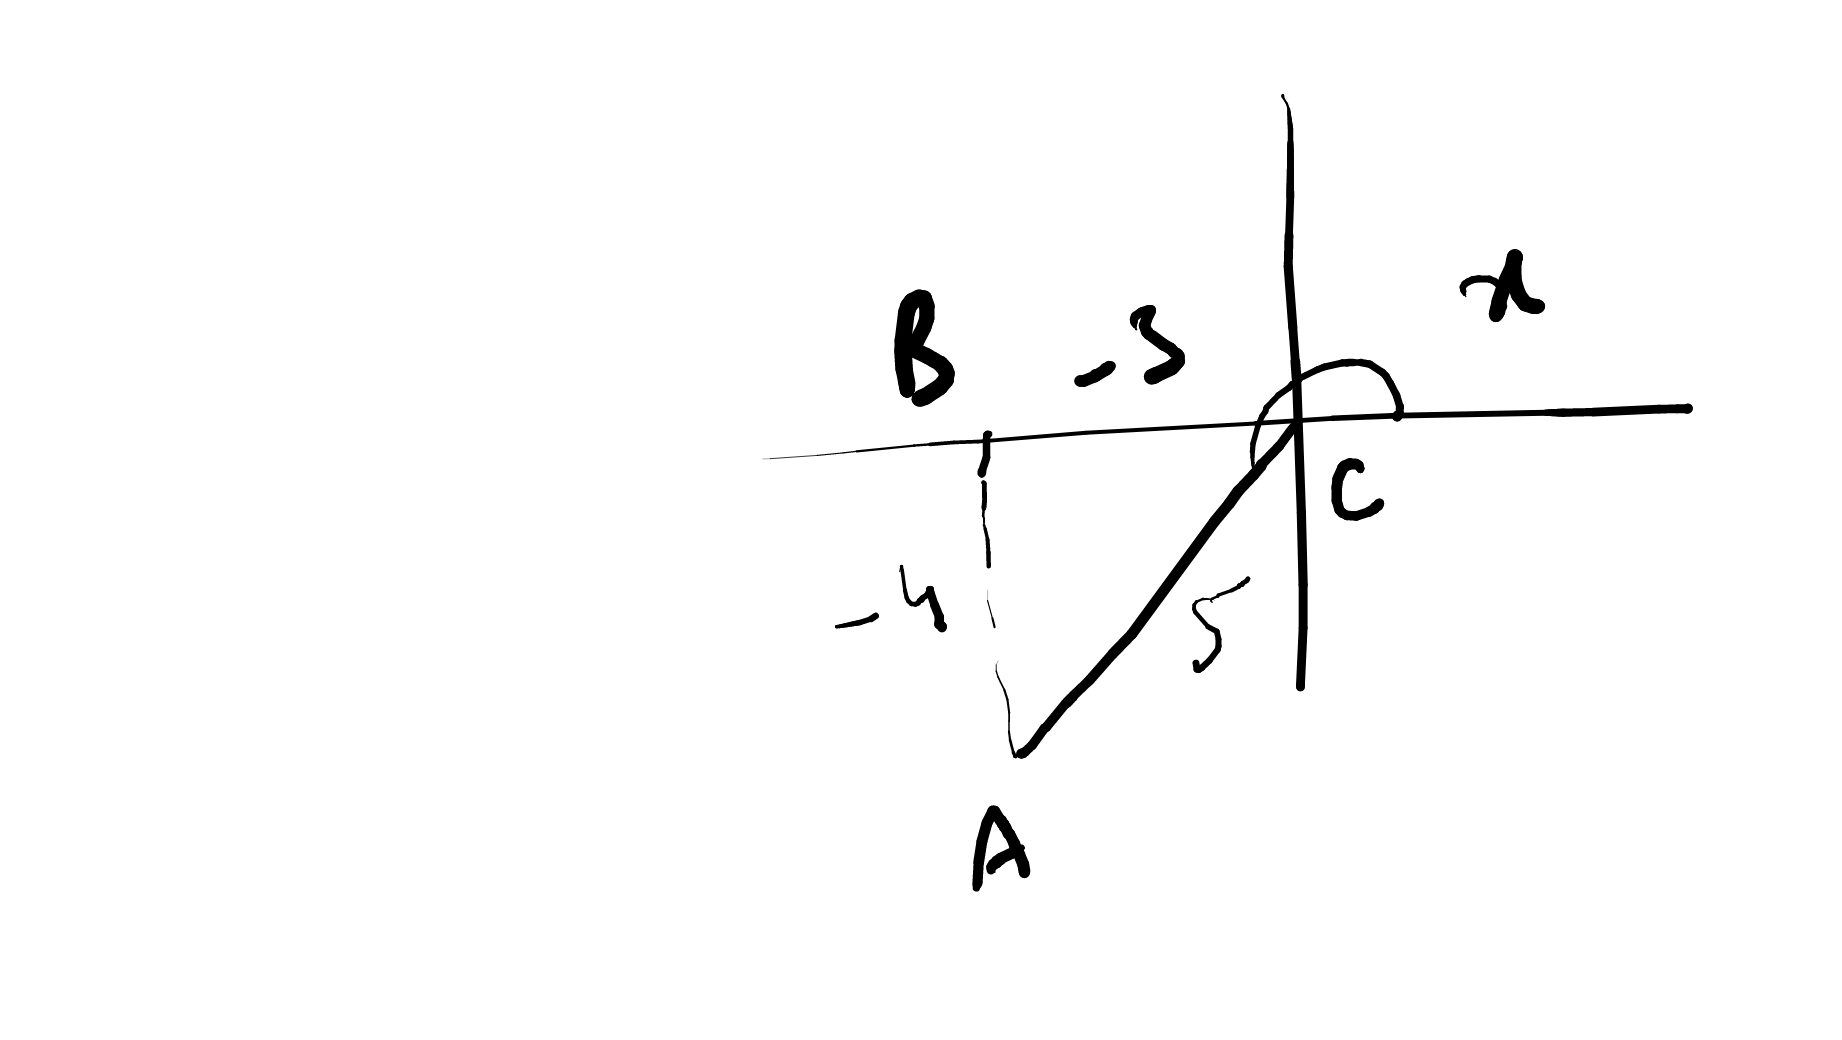
\includegraphics[width=0.6\columnwidth]{figs/ncert/id/1.png}}
	\end{center}
	\caption{}
	\label{fig:ncert-id-1}	
\end{figure}
\item If $\cot x = - \frac{5}{12}, x$ lies in the second quadrant, find the values of other five trigonometric function.
%
\\
\solution
	In \figref{fig:ncert-id-2}, 
\begin{align}
	a &= -5, b = 13, c = 12 
	\\
\implies \cos x &= -\frac{5}{13}\,
\sin x = \frac{12}{13}\,
\tan x = -\frac{12}{5}
\end{align}
\begin{figure}[H]
	\begin{center}
		{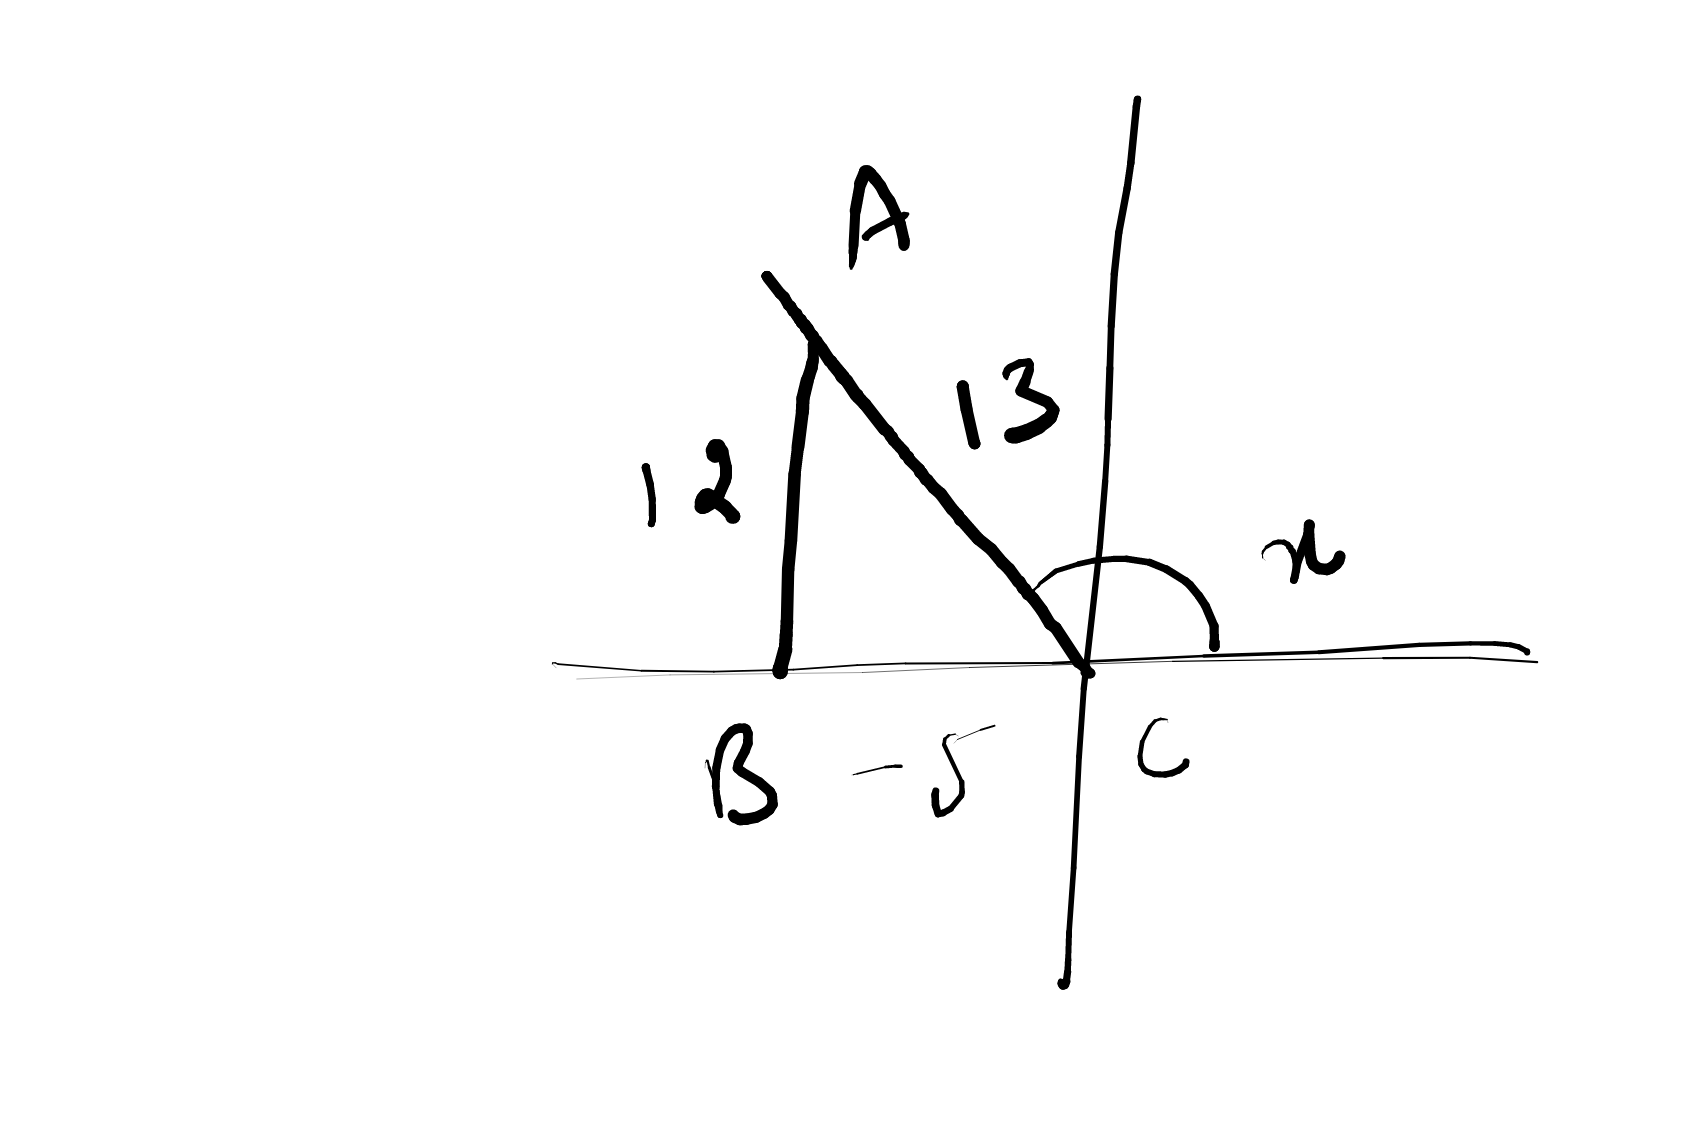
\includegraphics[width=0.6\columnwidth]{figs/ncert/id/2.png}}
	\end{center}
	\caption{}
	\label{fig:ncert-id-2}	
\end{figure}
\item Find the value of $\sin \frac{31\pi}{3}$.
%
	\\
		\solution 
\begin{align}
	\sin \frac{31\pi}{3} &= 
	\sin \brak{10 \pi+\frac{\pi}{3}} 
	\\
	&= 
	\sin \brak{\frac{\pi}{3}} = \frac{1}{2}
\end{align}
\item Find the value of $\cos\brak{-1710\degree}$.
%
	\\
		\solution 
\begin{align}
	\cos\brak{-1710\degree}	&= 
\cos\brak{-5\times360\degree+90\degree}	 
\\
	&=\cos{90\degree}	= 0
\end{align}
\item Prove that $3\sin\frac{\pi}{6}\sec\frac{\pi}{3}-4\sin\frac{5\pi}{6}\cot\frac{\pi}{4} = 1.$
%
	\\
	\solution
\begin{align}
	3\sin\frac{\pi}{6}\sec\frac{\pi}{3}-4\sin\frac{5\pi}{6}\cot\frac{\pi}{4} &= 
	3\frac{\sin\frac{\pi}{6}}{\cos\brak{\frac{\pi}{2}-\frac{\pi}{6}}}-4\sin\brak{\pi - \frac{\pi}{6}}  
	\\
	&=
	3\frac{\sin\frac{\pi}{6}}{\sin\frac{\pi}{6}}-4\sin\brak{ \frac{\pi}{6}}  
	= 1
\end{align}
upon substituting numerical values.
\item Find the value of $\sin 15\degree$.
%
	\\
	\solution 
\begin{align}
	1 - 2 \sin^2 15 &= \cos 30 = \frac{\sqrt{3}}{2}
	\\
	\implies 
	\sin 15 &= \sqrt{\frac{1-\frac{\sqrt{3}}{2}}{2}}
	 = \frac{\sqrt{2-\sqrt{3}}}{2}
	 \label{eq:id-sin15}
\end{align}
\item Find the value of $\tan\frac{13\pi}{12}$.
%
	\\
	\solution 
\begin{align}
\tan\frac{13\pi}{12}
	&=
	\tan\brak{\pi+\frac{\pi}{12}}
=\tan\frac{\pi}{12}
\end{align}
%
Since
\begin{align}
	2 \cos^2 15 -1 &= \cos 30 = \frac{\sqrt{3}}{2},
	\\
	\cos15 &= \sqrt{\frac{1+\frac{\sqrt{3}}{2}}{2}}
	 = \frac{\sqrt{2+\sqrt{3}}}{2}
	 \label{eq:id-cos15}
	 \\
	 \therefore 
	\tan\frac{\pi}{12} &= \frac{\sin 15}{\cos15}
	 = \frac{\sqrt{2-\sqrt{3}}}{\sqrt{2+\sqrt{3}}}
	 \label{eq:id-tan15}
\end{align}
upon substituting from 
	 \eqref{eq:id-sin15}.
\item Prove that 
\begin{align}
	\frac{\sin\brak{x+y}}{\sin\brak{x-y}} = \frac{\tan x + \tan y}{\tan x - \tan y}.
	 \label{eq:id-cosxcosy}
\end{align}
%
	\\
	\solution
\begin{align}
\frac{\sin\brak{x+y}}{\sin\brak{x-y}} = \frac{\sin x \cos y +\sin y \cos x }{\sin x \cos y -\sin y \cos x }
\end{align}
Dividing the numerator and denominator by $\cos x \cos y$
%
yields
	 \eqref{eq:id-cosxcosy}.
\item Show that
\begin{align}
	 \label{eq:id-tanx2x3x}
\tan3x\tan2x\tan x = \tan3x-\tan2x-\tan x
\end{align}
%
\\
\solution
\begin{align}
	\tan3x = \tan \brak{2x +\tan x} &= \frac{\tan 2x + \tan x}{1 - \tan x \tan 2x}
	\\
	\implies 
	\tan3x \brak{1 - \tan x \tan 2x}&= {\tan 2x + \tan x}
\end{align}
%
yielding
	 \eqref{eq:id-tanx2x3x}.
\item Prove that
\begin{align}
\cos\brak{\frac{\pi}{4}+x} + \cos\brak{\frac{\pi}{4}-x} = \sqrt 2\cos x.
	 \label{eq:id-sqrt2cosx}
\end{align}
%
\\
\solution
\begin{align}
\cos\brak{\frac{\pi}{4}+x} + \cos\brak{\frac{\pi}{4}-x} = 
2\cos\brak{\frac{\pi}{4}} \cos x  
\end{align}
yielding
	 \eqref{eq:id-sqrt2cosx}
	 after substituting numerical values.
%
\item Prove that 
%
\begin{align}
\frac{\cos7x+\cos5x}{\sin7x-\sin 5x} 
=\cot x
	 \label{eq:id-cotx}
\end{align}
%
\\
\solution
\begin{align}
\frac{\cos7x+\cos5x}{\sin7x-\sin 5x} 
=\frac{2\cos6x\cos x}{2\cos 6x\cos x} 
\end{align}
yielding
	 \eqref{eq:id-cotx}.
\item Prove that 
\begin{align}
	\frac{\sin5x-2\sin3x+\sin x}{\cos5x-\cos x} = \tan x.
	 \label{eq:id-tanx}
\end{align}
%
\\
\solution
\begin{align}
	\frac{\sin5x-2\sin3x+\sin x}{\cos5x-\cos x} 
	&=
	-\frac{2\sin3x\cos2x-2\sin3x}{2\sin 3x\sin 2x}
	\\
	&=
	\frac{1-\cos2x}{\sin2x} = \frac{2\sin^2 x}{2\sin x\cos x}
\end{align}
	 yielding \eqref{eq:id-tanx}.
%
\item If $\sin x=\frac{3}{5}, \cos y=-\frac{12}{13}$, where $x$ and $y$
both lies in second quadrant, find the value of
$\sin\brak{x+y}$.
%
\\
\solution 
From the given information,
\begin{align}
	\cos x &= -\frac{4}{5},
	\sin y = \frac{5}{13}
	\\
	\implies 
	\sin\brak{x+y} &= -\frac{3}{5}\times \frac{12}{13} - \frac{4}{5}\times \frac{5}{13}
	\\
	&=-\frac{56}{65}
\end{align}
%
\item Prove that
\begin{align}
\cos2x\cos\frac{x}{2}-\cos3x\cos\frac{9x}{2}=\sin5x\sin\frac{5x}{2}.
	 \label{eq:id-sin5x}.
\end{align}
%
\\
\solution 
\begin{align}
\cos2x\cos\frac{x}{2}
	&=\frac{1}{2}\brak{\cos\brak{2x+\frac{x}{2}}+\cos\brak{2x-\frac{x}{2}}}
	\\
\cos3x\cos\frac{9x}{2}
	&=\frac{1}{2}\brak{\cos\brak{3x+\frac{9x}{2}}+\cos\brak{3x-\frac{9x}{2}}}
\end{align}
Also,
\begin{align}
	\cos\brak{2x+\frac{x}{2}}-
\cos\brak{3x+\frac{9x}{2}}
	&= 2\sin 5x \sin \frac{5x}{2}
\\
\cos\brak{2x-\frac{x}{2}}
-
\cos\brak{3x-\frac{9x}{2}}
	&= 0
\end{align}
%
yielding
	 \eqref{eq:id-sin5x} after some algebra.
\item Find the value of $\tan\frac{\pi}{8}$.
%
	\\
	\solution
\begin{align}
	\tan 2\theta = \frac{2\tan \theta}{1-\tan^2\theta}
\label{eq:id-tantheta}
\end{align}
For $\theta = \frac{\pi}{8}$,  we obtain
\begin{align}
	 \frac{2\tan \theta}{1-\tan^2\theta}=1
	 \implies 
	{\tan^2\theta}+{2\tan \theta}- 1=0
\end{align}
yielding
\begin{align}
	\tan \theta = \sqrt{2}-1 
\end{align}
by taking the positive root of the quadratic.
%
\item If $\tan x=\frac{3}{4}, \pi<x<\frac{3\pi}{2}$, find the value of $\sin\frac{x}{2},\cos\frac{x}{2}$ and $\tan\frac{x}{2}$.
%
	\\
	\solution $ \frac{\pi}{2}<\frac{x}{2} <\frac{3\pi}{4} $, hence $\frac{x}{2}$
	lies in the $2^{nd}$
	quadrant.
%
	For $\theta = \frac{x}{2}$
	in
\eqref{eq:id-tantheta},
\begin{align}
	3{\tan^2\theta}+{8\tan \theta}- {3}=0
	\\
	\implies
	\tan\frac{x}{2}=\tan \theta = -3
\end{align}
by taking the negative root.
From
	\figref{fig:ncert-id-3},	
\begin{align}
	\cos \frac{x}{2} = -\frac{1}{\sqrt{10}},
	\sin\frac{x}{2} = \frac{3}{\sqrt{10}}
\end{align}
\begin{figure}[H]
	\begin{center}
		{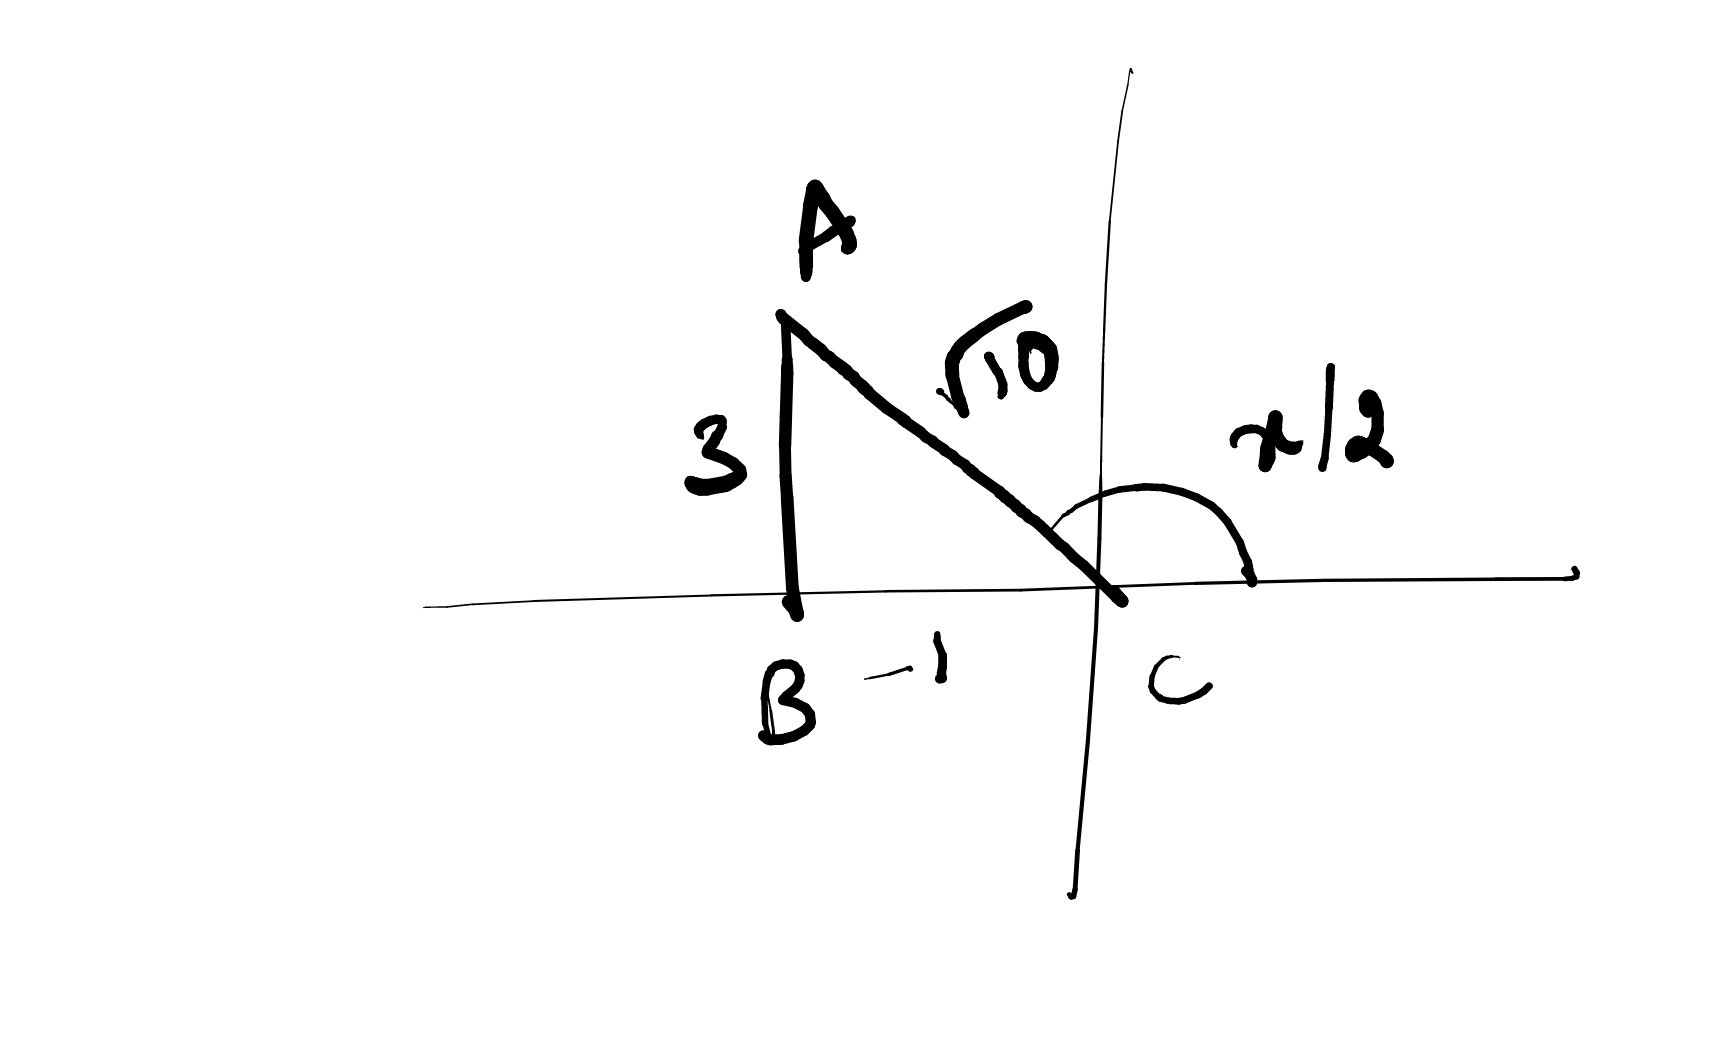
\includegraphics[width=0.6\columnwidth]{figs/ncert/id/3.png}}
	\end{center}
	\caption{}
	\label{fig:ncert-id-3}	
\end{figure}
\item Prove that
$\cos^{2}x+\cos^{2}\brak{x+\frac{\pi}{3}}+\cos^{2}\brak{x-\frac{\pi}{3}}=\frac{3}{2}$.
%
\\
\solution The LHS can be expressed as
\begin{multline}
	\frac{1 + \cos 2x + 1 + \cos\brak{2x+\frac{2\pi}{3}}+ 1+\cos\brak{2x-\frac{2\pi}{3}}}{2}
	\\
	=
	\frac{3}{2} +
	\frac{\cos 2x + 2\cos2x\cos \brak{\frac{2\pi}{3}}}{2}
\end{multline}
yielding the RHS upon substituting numerical values.
\item Find the values of other five trigonometric functions 
\begin{enumerate}
	\item $\cos x=-\frac{1}{2}$, $x$  lies in third quadrant.
	\item $\sin x= \frac{3}{5} $,$ x$  lies in second quadrant.
	\item $\cot x= \frac{3}{4}$,$ x$  lies in third quadrant.
	\item $\sec x= \frac{13}{5}$, $x$  lies in fourth quadrant.
	\item $\tan x=-\frac{5}{12}$, $x$  lies in second quadrant.
\end{enumerate}
%
\solution
\begin{enumerate}
	\item 
	See \figref{fig:ncert-id-4}.	
\begin{align}
	\sin x = -\frac{\sqrt{3}}{2},
	\tan x = {\sqrt{3}}
\end{align}
\begin{figure}[H]
	\begin{center}
		{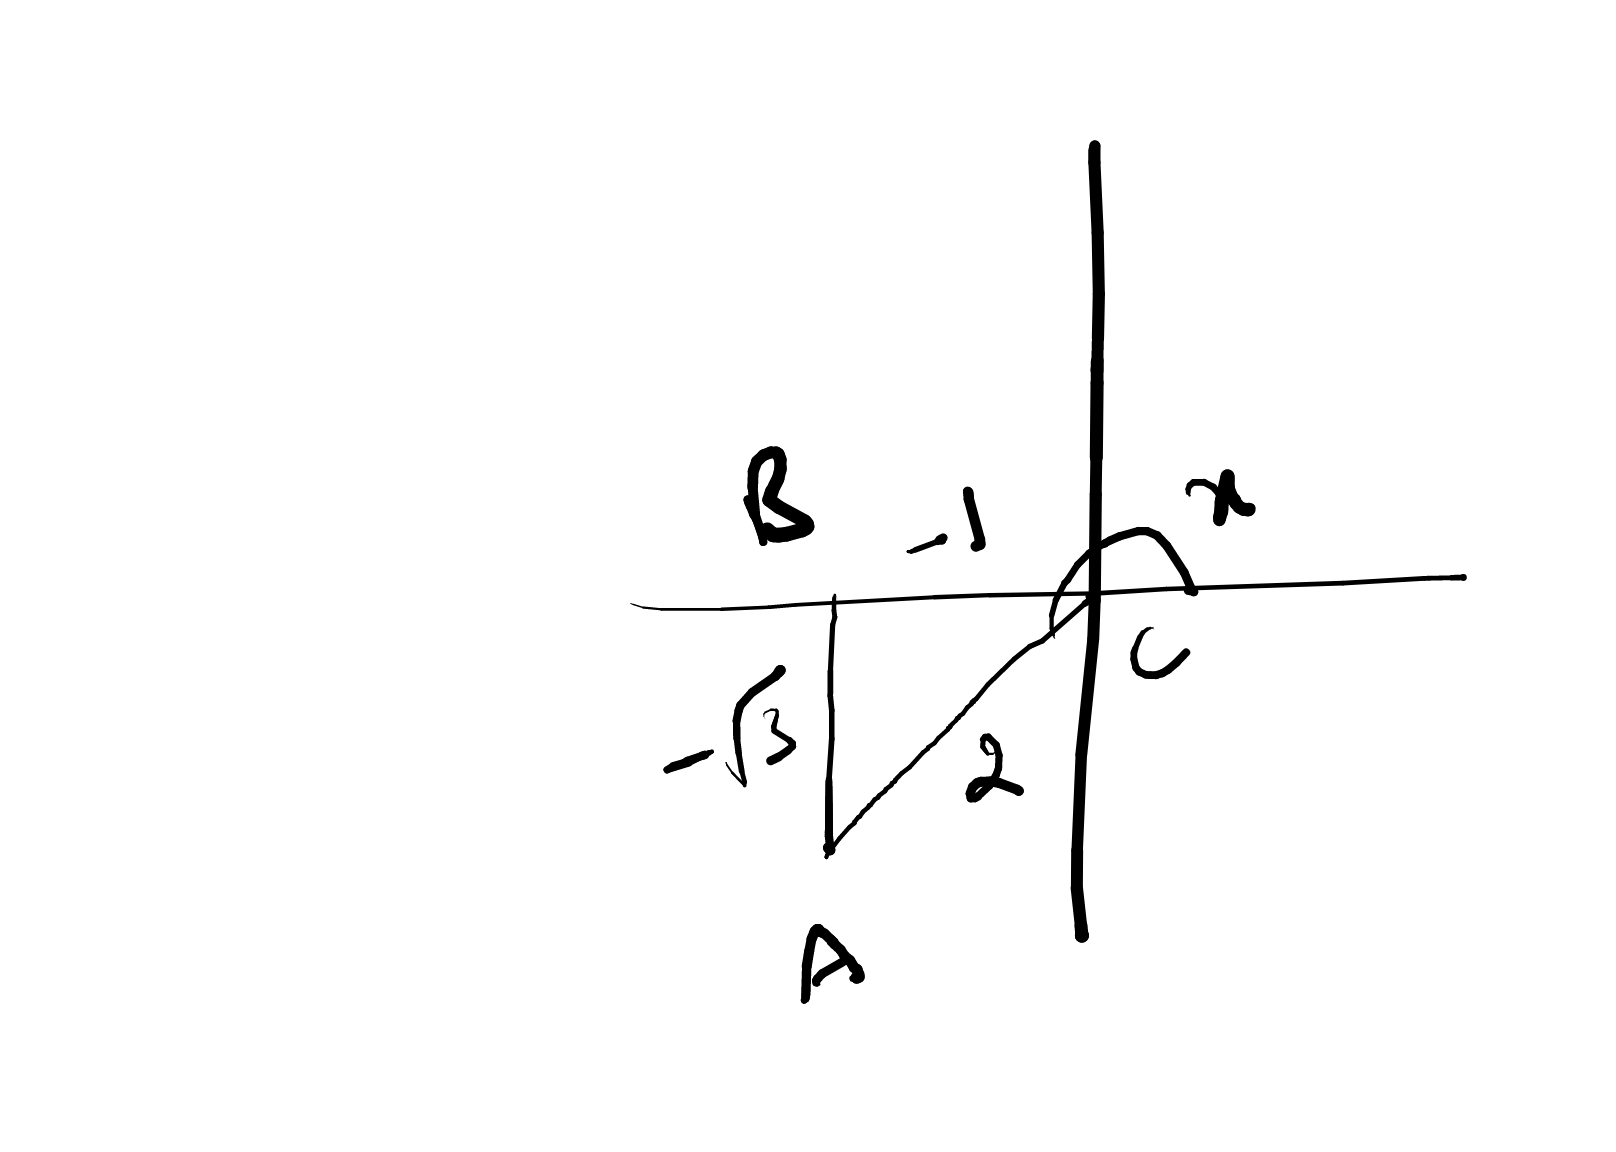
\includegraphics[width=0.6\columnwidth]{figs/ncert/id/4.png}}
	\end{center}
	\caption{}
	\label{fig:ncert-id-4}	
\end{figure}
	\item 
	See \figref{fig:ncert-id-5}.	
\begin{align}
	\cos x = -\frac{4}{5},
	\tan x = -\frac{3}{4}.
\end{align}
\begin{figure}[H]
	\begin{center}
		{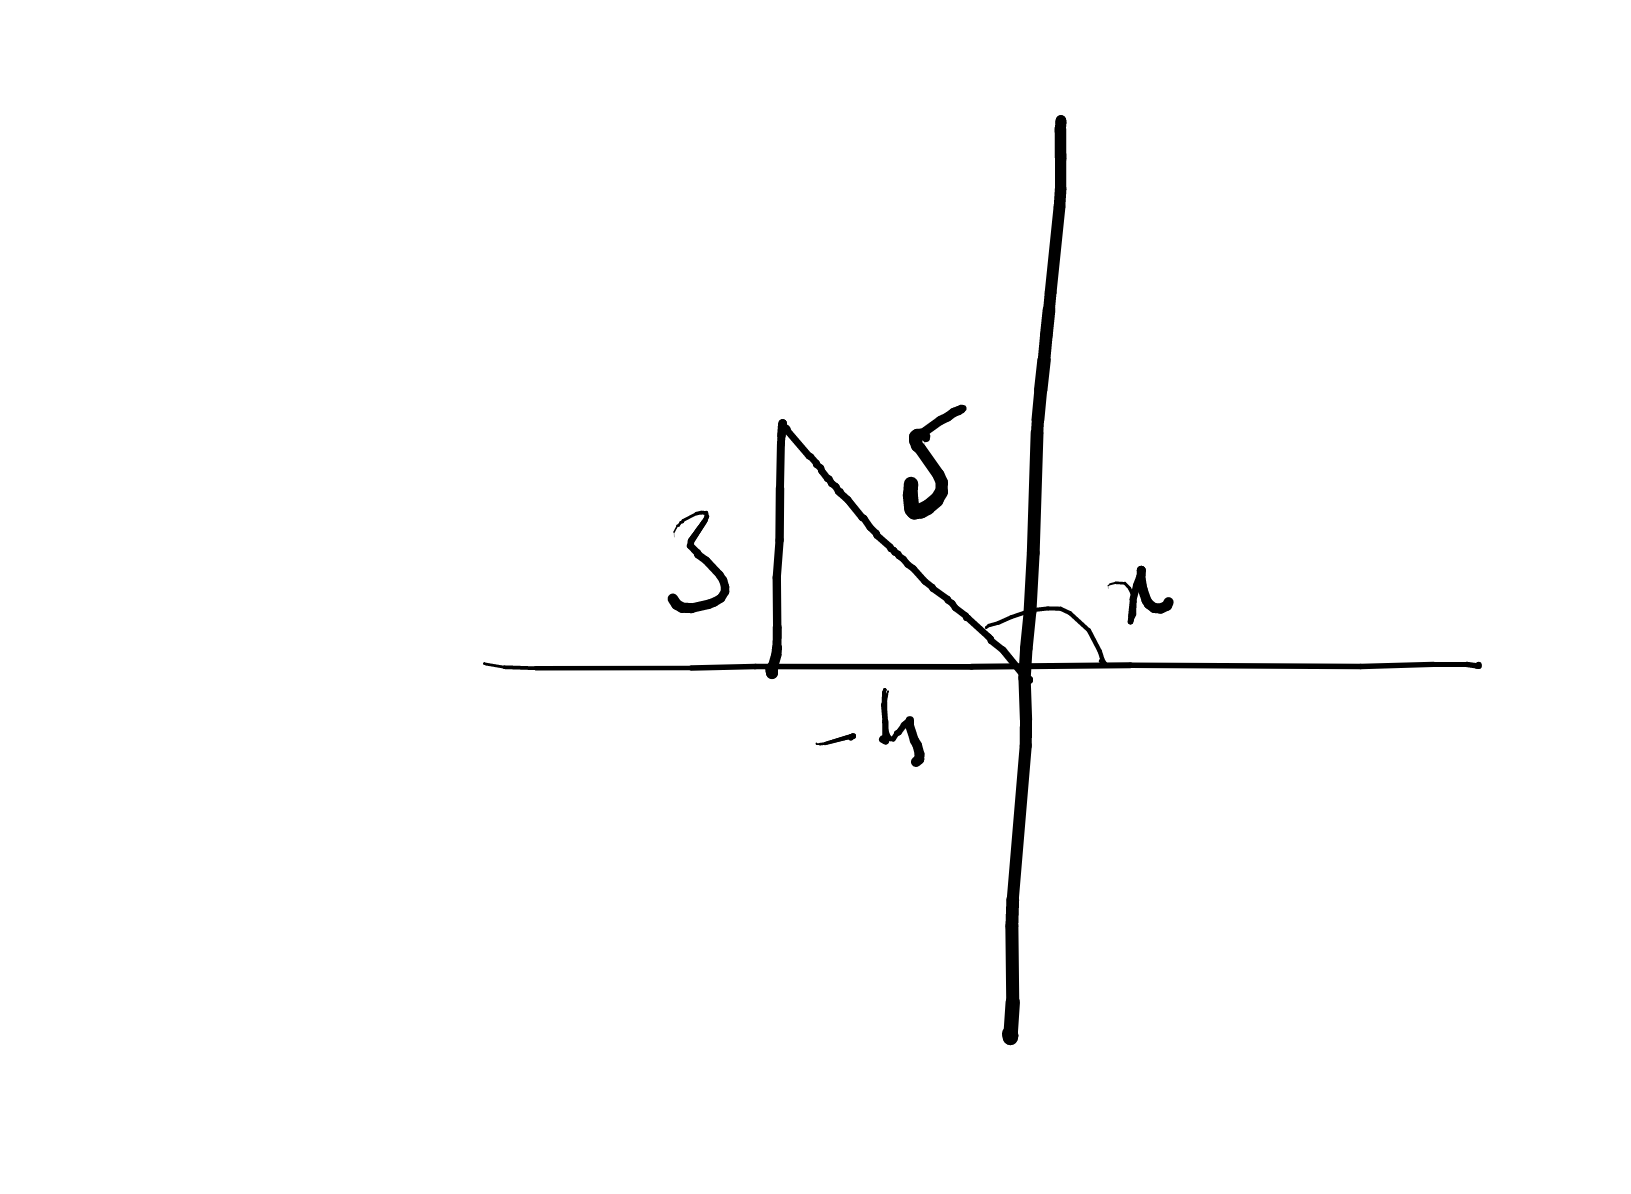
\includegraphics[width=0.6\columnwidth]{figs/ncert/id/5.png}}
	\end{center}
	\caption{}
	\label{fig:ncert-id-5}	
\end{figure}
	\item 
	See \figref{fig:ncert-id-6}.
\begin{align}
	\cos x = -\frac{3}{5},
	\sin x = -\frac{4}{5},
	\tan x = \frac{4}{3}.
\end{align}
\begin{figure}[H]
	\begin{center}
		{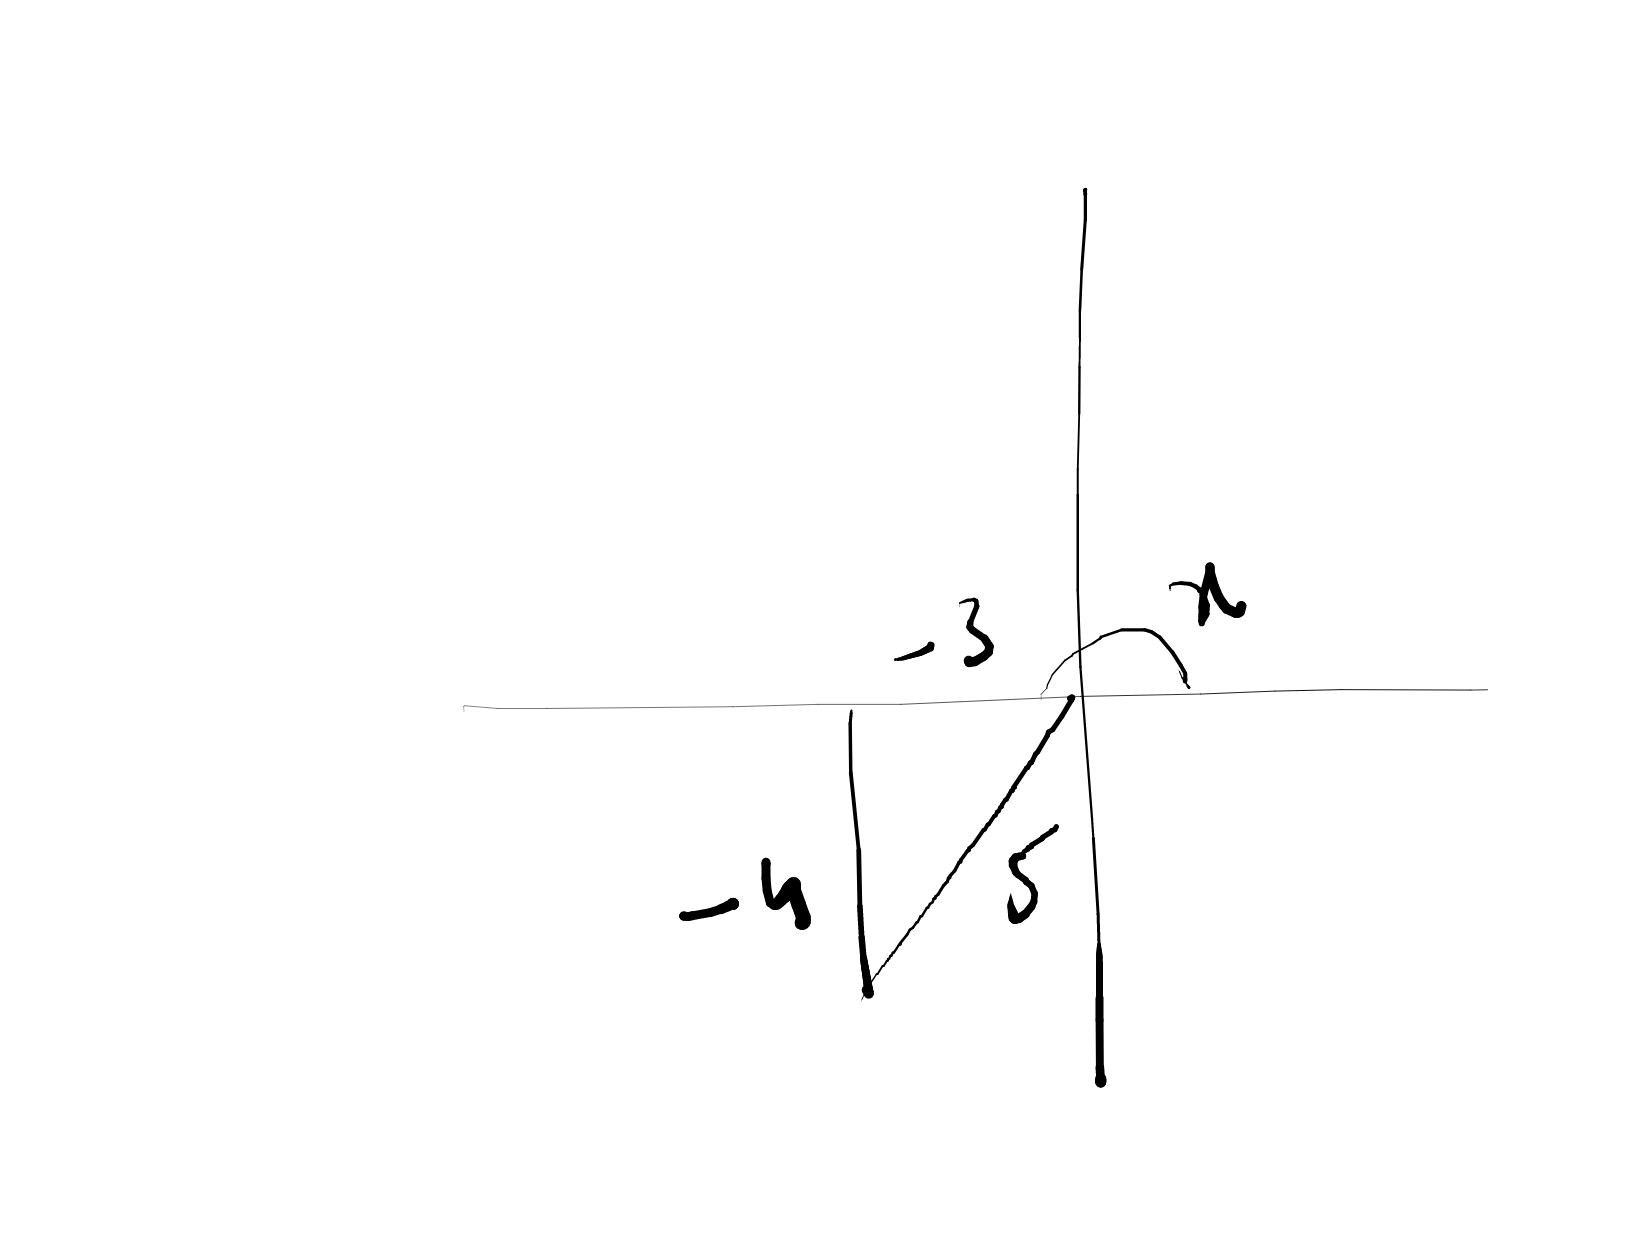
\includegraphics[width=0.6\columnwidth]{figs/ncert/id/6.png}}
	\end{center}
	\caption{}
	\label{fig:ncert-id-6}	
\end{figure}
	\item 
	See \figref{fig:ncert-id-7}.	
\begin{align}
	\cos x = \frac{5}{13},
	\sin x = -\frac{12}{13},
	\tan x = -\frac{12}{5}.
\end{align}
\begin{figure}[H]
	\begin{center}
		{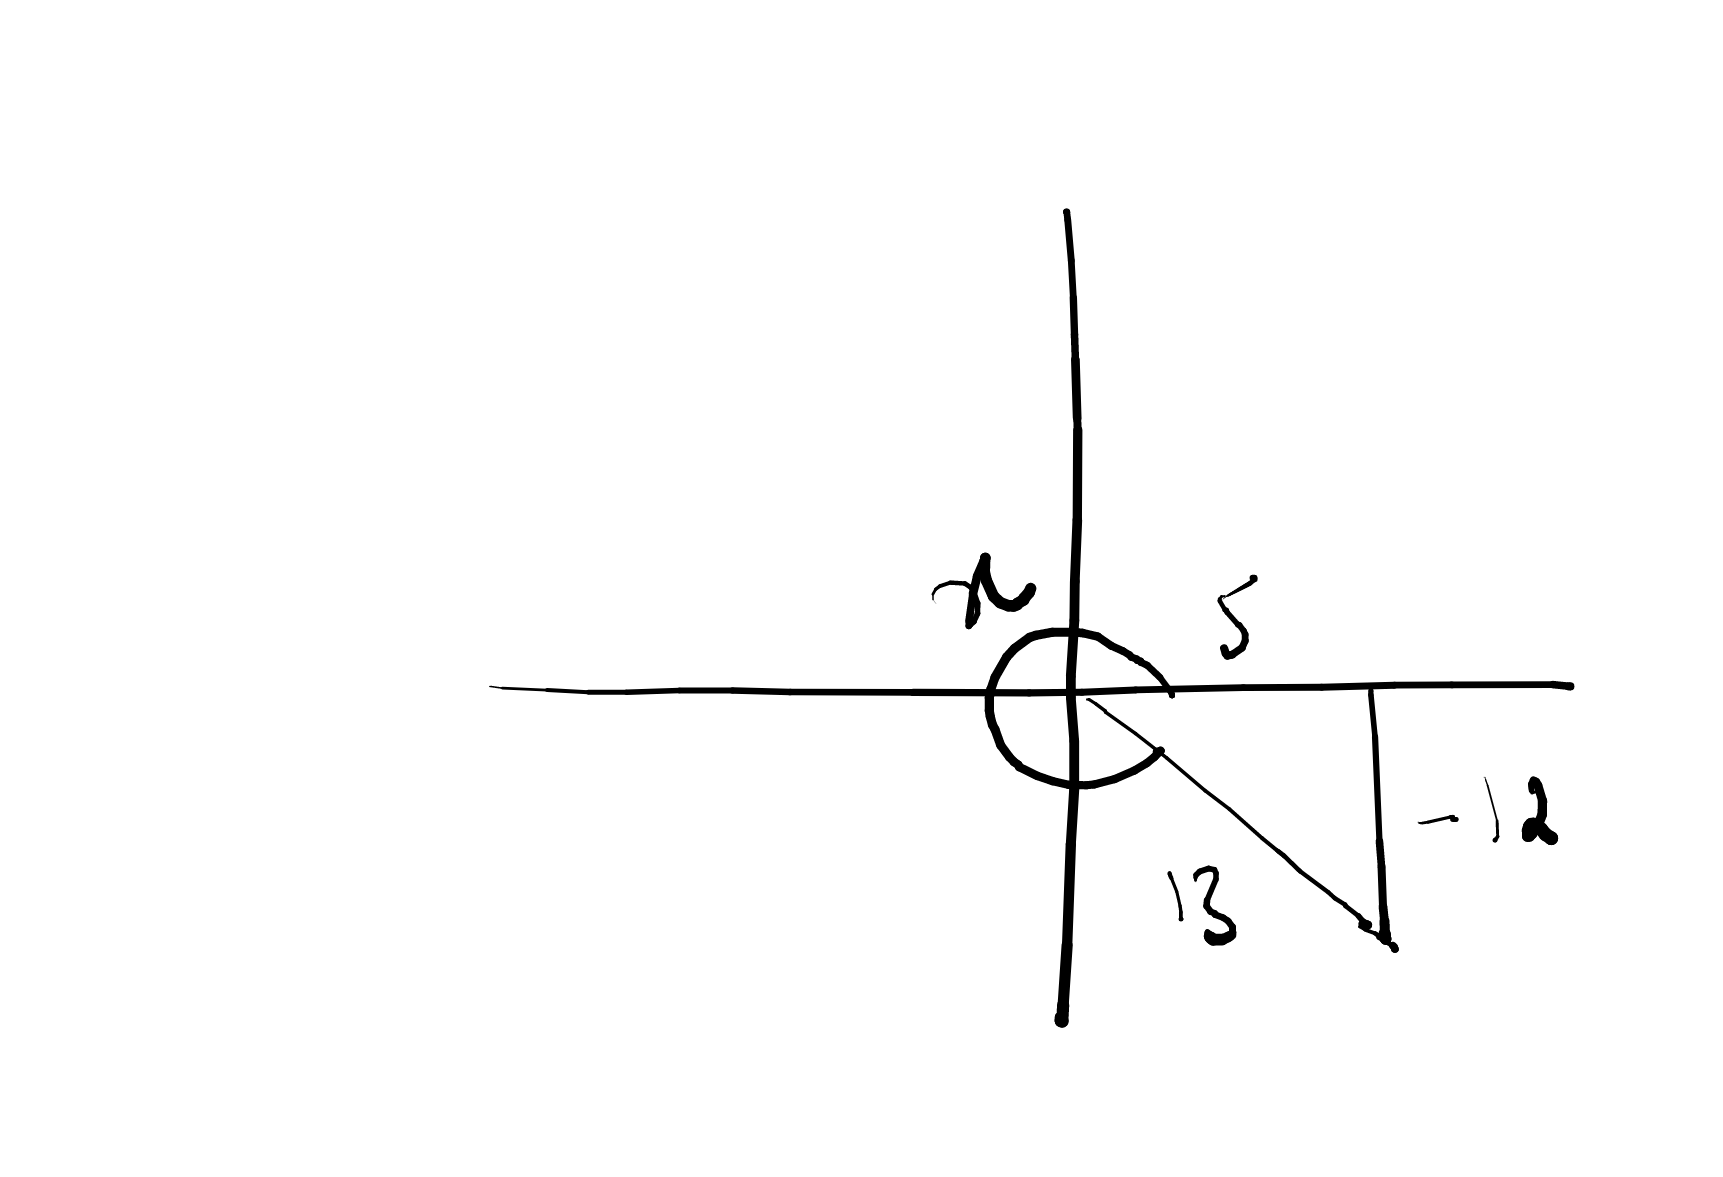
\includegraphics[width=0.6\columnwidth]{figs/ncert/id/7.png}}
	\end{center}
	\caption{}
	\label{fig:ncert-id-7}	
\end{figure}
	\item 
	See \figref{fig:ncert-id-8}.	
\begin{align}
	\cos x = -\frac{12}{13},
	\sin x = \frac{5}{13}
\end{align}
\begin{figure}[H]
	\begin{center}
		{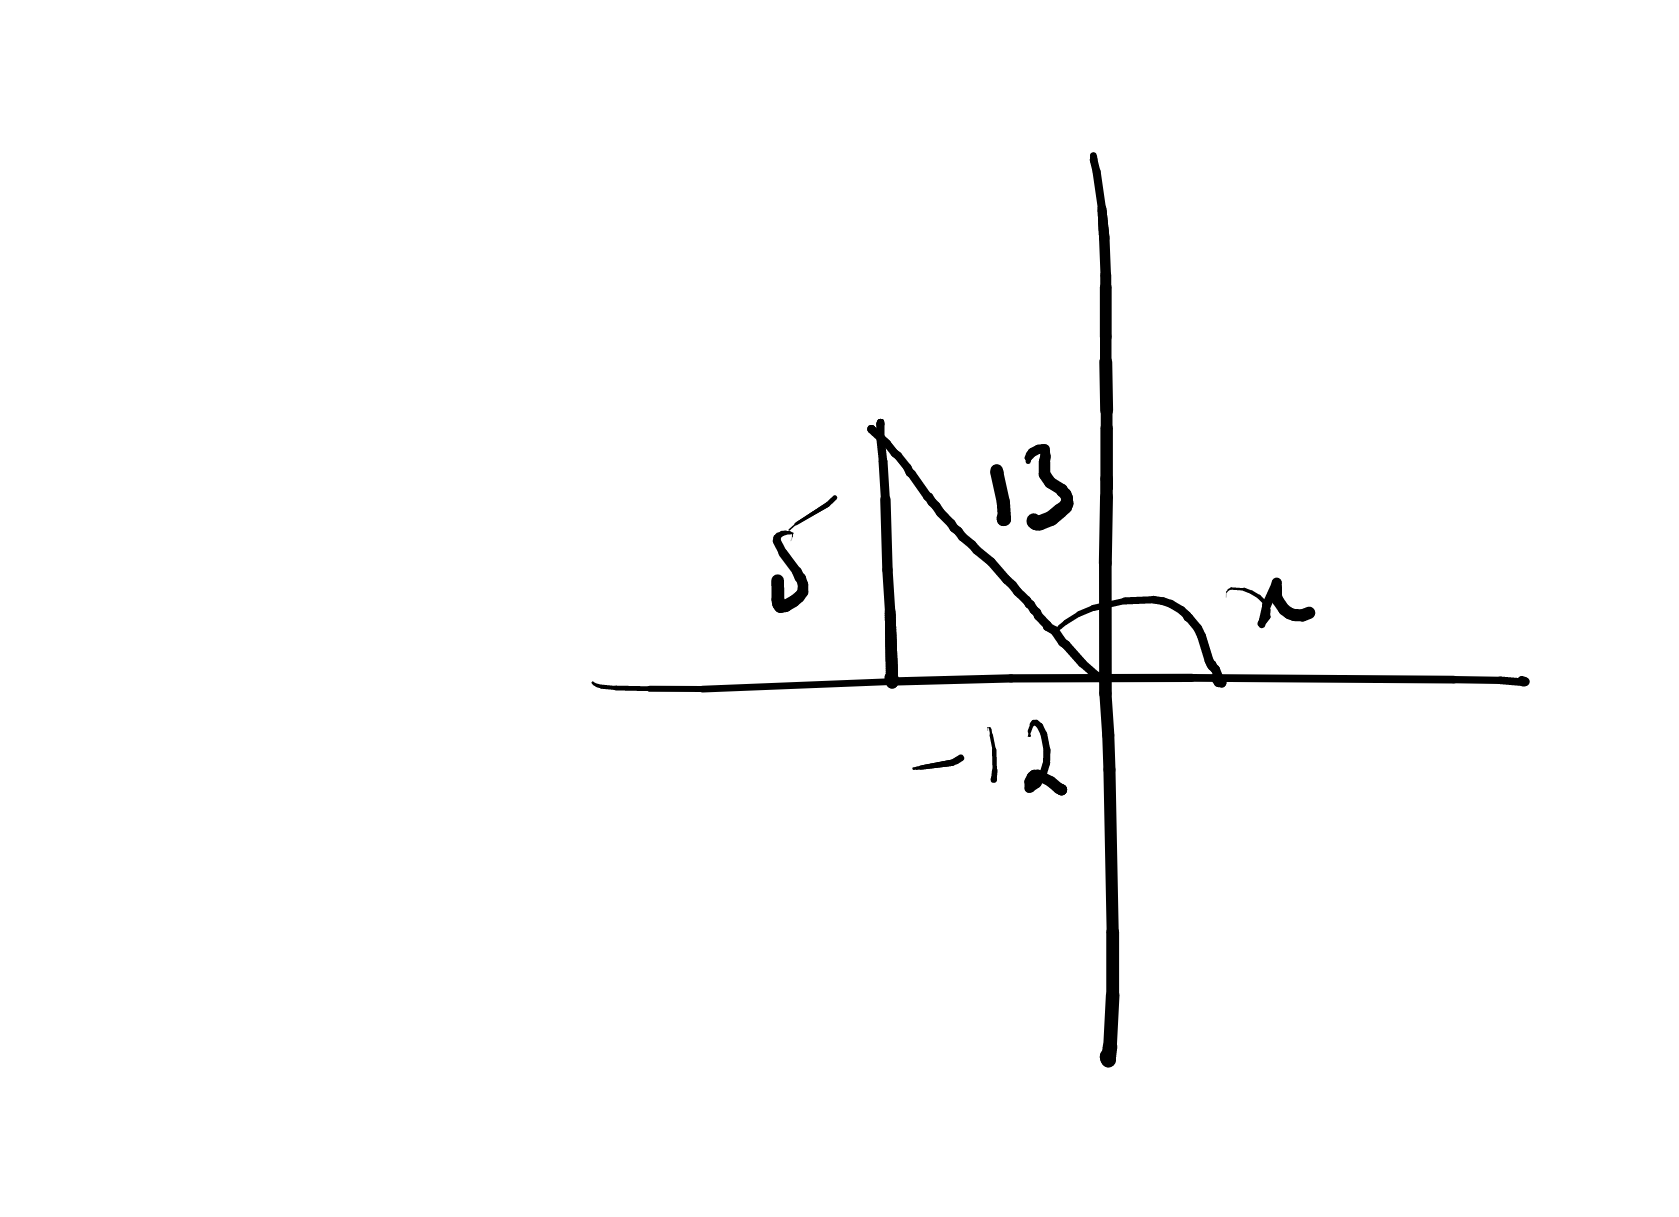
\includegraphics[width=0.6\columnwidth]{figs/ncert/id/8.png}}
	\end{center}
	\caption{}
	\label{fig:ncert-id-8}	
\end{figure}
\end{enumerate}
\item Find the values of the trigonometric functions
\begin{multicols}{2}
\begin{enumerate}
\item $\sin765\degree$
\item $\csc\brak{-1410\degree}$
\item $\tan\frac{19\pi}{3}$
\item $\sin\frac{-11\pi}{3}$
\item $\cot\frac{-15\pi}{4}$
\end{enumerate}
\end{multicols}
%
\solution
\begin{enumerate}
\item 
\begin{align}
	\sin765\degree &= \sin \brak{2\times 360\degree + 45 \degree}
	\\
	&= \sin 45\degree = \frac{1}{\sqrt{2}}
\end{align}
\item 
\begin{align}
	\csc\brak{-1410\degree}&=	
\csc\brak{-4\times 360\degree + 30 \degree}
\\
	&= \csc 30 \degree = {2}
\end{align}
\item 
\begin{align}
\tan\frac{19\pi}{3}
	&=	
	\tan\brak{6\pi + \frac{\pi}{3}}
	\\
	&= \tan \frac{\pi}{3}= {\sqrt{3}}
\end{align}
\item 
\begin{align}
\sin\frac{-11\pi}{3}
	&=\sin\brak{-4\pi +\frac{\pi}{3}}
	\\
	&=\sin{\frac{\pi}{3}}=\frac{\sqrt{3}}{2}
\end{align}
\item $\cot\frac{-15\pi}{4}$
\begin{align}
\cot\frac{-15\pi}{4}
	&=\cot\brak{-4\pi+\frac{\pi}{4}}
	\\
	&=\cot{\frac{\pi}{4}}=1
\end{align}
\end{enumerate}
\item Prove that
\begin{multicols}{2}
\begin{enumerate}
\item $\sin^{2}\frac{\pi}{6}+\cos^{2}\frac{\pi}{3}-\tan^{2}\frac{\pi}{4}=-\frac{1}{2}$
\item $2\sin^{2}\frac{\pi}{6}+\csc^{2}\frac{7\pi}{6}\cos^{2}\frac{\pi}{3}=\frac{3}{2}$
\item $\cot^{2}\frac{\pi}{6}+\csc\frac{5\pi}{6}+3\tan^{2}\frac{\pi}{6}$=6
\item $2\sin^{2}\frac{3\pi}{4}+2\cos^{2}\frac{\pi}{4}+2\sec^{2}\frac{\pi}{3}$=10
\end{enumerate}
\end{multicols}
%
\solution
\begin{enumerate}
\item The LHS is
\begin{align}
\sin^{2}\frac{\pi}{6}+\sin^{2}\frac{\pi}{6}-1
	&=
\sin^{2}\frac{\pi}{6}-\cos^{2}\frac{\pi}{6}
\\
	&=-\cos\frac{\pi}{3}=-\frac{1}{2}
\end{align}
\item The LHS can be expressed as
\begin{align}
	2\sin^{2}\frac{\pi}{6}+\frac{\cos^{2}\frac{\pi}{3}}{\sin^{2}\brak{\pi +\frac{\pi}{6}}} &= 
	2\sin^{2}\frac{\pi}{6}+\frac{\sin^{2}\frac{\pi}{6}}{\sin^{2}{\frac{\pi}{6}}} = \frac{1}{2} + 1 
\end{align}
\item The LHS equals
\begin{align}
	\tan^{2}\frac{\pi}{6}+\cot^{2}\frac{\pi}{6}+\csc\brak{\pi-\frac{\pi}{6}}+2\tan^{2}\frac{\pi}{6}
	&=
	\brak{\tan\frac{\pi}{6}+\cot\frac{\pi}{6}}^2-2+\csc{\frac{\pi}{6}}+2\tan^{2}\frac{\pi}{6}
	\\
	&=
	\sec^2\frac{\pi}{6}\csc^2\frac{\pi}{6}-2+2+2\tan^{2}\frac{\pi}{6}
	\\
	&=
	4\sec^2\frac{\pi}{6}+2\tan^{2}\frac{\pi}{6}
	\\
	&=
	4+6\tan^2\frac{\pi}{6} = 6
\end{align}
\item The LHS can be expressed as
\begin{align}
	2\sin^{2}\brak{\pi -\frac{\pi}{4}}+2\cos^{2}\frac{\pi}{4}+2\sec^{2}\frac{\pi}{3} &= 
	2\brak{\sin^{2}\frac{\pi}{4}+\cos^{2}\frac{\pi}{4}}+8
\end{align}
\end{enumerate}
\item Find the value of
\begin{multicols}{2}
\begin{enumerate}
\item$\sin75\degree$
\item $\tan15\degree$
\end{enumerate}
\end{multicols}
%
\solution
\begin{enumerate}
\item 
\begin{align}
\sin 75\degree 
=\cos 15\degree 
\end{align}
	 which is available in \eqref{eq:id-cos15}.
\item See
	 \eqref{eq:id-tan15}.
\end{enumerate}
\item Prove that 
 $\cos\brak{\frac{\pi}{4}-x}\cos\brak{\frac{\pi}{4}-y}-\sin\brak{\frac{\pi}{4}-x}\sin\brak{\frac{\pi}{4}-y}=\sin\brak{x+y}$.
%
 \\
 \solution
 The LHS can be expressed as
\begin{align}
	\cos\brak{\frac{\pi}{4}-x+\frac{\pi}{4}-y}&=\cos\sbrak{\frac{\pi}{2}-\brak{x+y}}
\end{align}
which is equal to the RHS.
\item Prove that 
$$\frac{\tan\brak{\frac{\pi}{4}+x}}{\tan\brak{\frac{\pi}{4}-x}}=\brak{\frac{1+\tan x}{1-\tan x}}^{2}.$$
%
\solution
\begin{align}
	{\tan\brak{\frac{\pi}{4}+x}}&=\frac{\tan\frac{\pi}{4}+\tan x}{1-\tan\frac{\pi}{4}\tan x}
	\\
	&=\frac{1+\tan x}{1-\tan x}
	\\
{\tan\brak{\frac{\pi}{4}-x}}&=\frac{\tan\frac{\pi}{4}-\tan x}{1+\tan\frac{\pi}{4}\tan x}
	\\
	&=\frac{1-\tan x}{1+\tan x}
\end{align}
From the above, the desired result is obtained.
\item Prove that
$$\frac{\cos\brak{\pi+x}\cos\brak{-x}}{\sin\brak{\pi-x}\cos\brak{\frac{\pi}{2}+x}}=\cot^{2}x.$$
%
\solution
The LHS can be expressed as
\begin{align}
	\frac{-\cos x\cos\brak{-x}}{\sin x\brak{-\sin x}}
\end{align}
yielding the RHS.
\item Prove that
$\cos\brak{\frac{3\pi}{2}+x}\cos\brak{2\pi+x}\sbrak{\cot\brak{\frac{3\pi}{2}-x}+\cot\brak{2\pi +x}}=1$.
%
\\
\solution The LHS can be expressed as 
\begin{align}
	\sin x\cos x\sbrak{\tan x+\cot x}=
\sin x\cos x\sec x\csc x
\end{align}
yielding the RHS.
\item Prove that
$\sin\brak{n+1}x\sin\brak{n+2}x+\cos\brak{n+1}x\cos\brak{n+2}x=\cos x.$
%
\\
\solution The LHS can be expressed as
\begin{align}
	\frac{1}{2}\sbrak{\cos x - \cos\brak{\frac{n+3}{2}x}+\cos x+\cos\brak{\frac{n+3}{2}x}}
\end{align}
yielding the RHS.
\item Prove that
$\cos\brak{\frac{3\pi}{4}+x}-\cos\brak{\frac{3\pi}{4}-x}=-\sqrt 2\sin x.$
%
\\
\solution  The LHS can be expressed as 
\begin{align}
-2\sin x \sin \frac{3\pi}{4}
=-2\sin x \sin \frac{\pi}{4}
\end{align}
yielding the RHS.
\item Prove that
$\sin^{2}6x-\sin^{2}4x=\sin2x\sin10x.$
%
\\
\solution  The LHS can be expressed as 
\begin{align}
	\frac{\cos 8x - \cos 12 x }{2}
\end{align}
yielding the RHS.
\item Prove that
$\cos^{2}2x-\cos^{2}6x=\sin4x\sin8x.$
%
\\
\solution  The LHS can be expressed as 
\begin{align}
	\frac{\cos 4x - \cos 12 x }{2}
\end{align}
yielding the RHS.
\item Prove that
$\sin2x+2\sin4x+\sin6x=4\cos^{2}x\sin4x.$
%
\\
\solution  The LHS can be expressed as 
\begin{align}
	\sin2x+\sin6x+2\sin4x&=2\sin4x\cos 2x + 2\sin 4x
	\\
	&=2\sin4x\brak{1+\cos 2x} 
\end{align}
yielding the RHS.
\item Prove that
$\cot4x\brak{\sin5x+\sin3x}= \cot x\brak{\sin5x-\sin3x}.$
%
\\
\solution  
\begin{align}
	LHS = 
2\cot4x\sin4x\cos x
\\
	&= 
2\cos4x\sin x
	\\
	RHS&=2\cot x\cos 4x \sin x
\end{align}
\item Prove that
$$\frac{\cos9x-\cos5x}{\sin17x-\sin3x}=-\frac{\sin2x}{\cos10x}.$$
%
\solution
\begin{align}
LHS = -\frac{2 \sin7x\sin 2x}{2\cos 10x\sin7x}
=RHS
\end{align}
\item Prove that
$$\frac{\sin5x+\sin3x}{\cos5x+\cos3x}=\tan4x.$$
%
\solution
\begin{align}
LHS = \frac{2\sin4x\cos 2x}{2\cos4x\cos2x}=RHS
\end{align}
\item Prove that
$$\frac{\sin x-\sin y}{\cos x+\cos y}=\tan\brak{\frac{x-y}{2}}.$$
%
\solution 
\begin{align}
LHS = \frac{2\sin \brak{\frac{x+y}{2}}\cos\brak{\frac{x-y}{2}}}{2\cos\brak{\frac{x+y}{2}}\cos\brak{\frac{x-y}{2}}}=RHS
\end{align}
\item Prove that
$$\frac{\sin x+\sin3x}{\cos x+\cos3x}=\tan2x.$$
%
\solution 
\begin{align}
	LHS=
\frac{2\sin 2x \cos x}{2\cos 2x\cos x}=RHS
\end{align}
\item Prove that
$$\frac{\sin x-\sin3x}{\sin^{2}x-\cos^{2}x}=2\sin x.$$
%
\solution
\begin{align}
LHS = \frac{-2\sin x\cos2x}{-\cos{2}x}=RHS
\end{align}

\item Prove that
$$\frac{\cos4x+\cos3x+\cos2x}{\sin4x+\sin3x+\sin2x}=\cot3x.$$
%
\solution
\begin{align}
LHS &= \frac{2\cos3x\cos x+\cos3x}{2\sin3x\cos x+\sin3x}
\\
&= \frac{\cos3x\brak{\cos x+1}}{\sin3x\brak{\cos x+1}}
=RHS
\end{align}
\item Prove that
\begin{align}
\cot x\cot2x-\cot2x\cot3x-\cot3x\cot x=1.
\label{eq:cot}
\end{align}
%
\\
\solution
\begin{align}
	\cot x  = \cot\brak{3x-2x} &= \frac{\cot 3x \cot 2x +1}{\cot 2x - \cot 3x}
	\\
	\implies 
\cot x\cot2x-\cot3x\cot x &=1+\cot2x\cot3x
\end{align}
yielding  
\eqref{eq:cot}.
\item Prove that
\begin{align}
\tan4x=\frac{4\tan x\brak{1-\tan^{2}x}}{1-6\tan^{2}x+\tan^{4}x}.
\label{eq:tan4x-ans}
\end{align}
%
\solution
\begin{align}
\label{eq:tan4x}
\tan 4x &= 
 \frac{2\tan 2x}{1-\tan^{2} 2x}
 \\
\tan 2x &= 
 \frac{2\tan x}{1-\tan^{2} x}
\label{eq:tan2x}
\end{align}
Substituting \eqref{eq:tan4x}
in \eqref{eq:tan4x}
yileds
\eqref{eq:tan4x-ans}.
\item Prove that
\begin{align}
\label{eq:cos4x}
\cos4x=1-8\sin^{2}x\cos^{2}x.
\end{align}
%
\solution
\begin{align}
	\cos 4x  &= 1 - 2 \sin^2 2x
	\\
	&=1 - 2 \brak{2 \sin x \cos x}^2 = RHS
\end{align}
\item Prove that
\begin{align}
\label{eq:cos6x}
\cos6x=32\cos^{6}x-48\cos^{4}x+18\cos^{2}x-1.
\end{align}
%
\solution
\begin{align}
	\cos 6x&= 4 \cos^3 2x - 3 \cos 2x 
	\\
	&= 4 \brak{2 \cos^2 x - 1}^3 - 3 \brak{2\cos^2 x - 1} = RHS
\end{align}

after some algebra.
%
\item Prove that
\begin{enumerate}
\item 2$\cos\frac{\pi}{13}\cos\frac{9\pi}{13}+\cos\frac{3\pi}{13}+\cos\frac{5\pi}{13}=0$
\item $\brak{\sin3x+\sin x}\sin x+\brak{\cos3x-\cos x}\cos x=0$
\item $\brak{\cos x+\cos y}^{2}+\brak{\sin x-\sin y}^{2}=4\cos^{2}\brak{\frac{x+y}{2}}$
\item $\brak{\cos x-\cos y}^{2}+\brak{\sin x-\sin y}^{2}=4\sin^{2}\brak{\frac{x-y}{2}}$
\item $\sin x+\sin3x+\sin5x+\sin7x=4\cos x\cos2x\sin4x$
\item $$\frac{\brak{\sin7x+\sin5x}+\brak{\sin9x+\sin3x}}{\brak{\cos7x+\cos5x}+\brak{\cos9x+\cos3x}}=\tan6x$$
\item $\sin3x+\sin2x-\sin x=4\sin x\cos\frac{x}{2}\cos\frac{3x}{2}$
\end{enumerate}
%
\solution 
\begin{enumerate}
\item 
\begin{align}
	LHS &= 	2\cos\frac{\pi}{13}\cos\frac{9\pi}{13}+2\cos\frac{4\pi}{13}\cos\frac{\pi}{13}
	\\
	&=
		2\cos\frac{\pi}{13}\brak{\cos\frac{9\pi}{13}+2\cos\frac{4\pi}{13}}
		\\
		&=
		4\cos\frac{\pi}{13}\brak{\cos\frac{\pi}{2}\cos\frac{5\pi}{26}}=RHS. 
\end{align}
\item 
\begin{align}
	LHS &= \cos x\cos3x +\sin x\sin3x+ \sin^2 x-\cos^2 
	\\
	 &= \cos 2x - \cos 2x  = RHS
\end{align}
\item 
\begin{align}
	LHS &= \cos^{2} x+\cos^{2} y+\sin ^{2}x+\sin ^{2}y
	+2\brak{\cos x\cos y-\sin x\sin y}
 \\
	&=2 
	+2\cos\brak{ x+ y} = RHS
\end{align}
\item 
\begin{align}
	LHS &= \cos^{2} x+\cos^{2} y+\sin ^{2}x+\sin ^{2}y
	-2\brak{\cos x\cos y+\sin x\sin y}
 \\
	&=2 
	-2\cos\brak{ x+ y} = RHS
\end{align}
\item 
\begin{align}
	LHS&=\sin x+\sin7x+\sin3x+\sin5x
\\
	&=
2\sin 4x\cos3x+2\sin4x\sin x
\\
	&=
	2\sin 4x\brak{\cos3x+\sin x}=RHS
\end{align}
\item 
\begin{align}
	LHS&=\frac{2\sin6x\cos x+2\sin6x\cos3x}{2\cos6x\cos x+2\cos6x\cos3x}
	\\
	&=\frac{\sin6x\brak{\cos x+\cos3x}}{\cos6x\brak{\cos x+\cos3x}}
	=RHS
\end{align}
\item 
\begin{align}
	LHS &= \sin3x+\sin2x-\sin x
	\\
	 &= 2\sin\frac{3x}{2}\cos\frac{3x}{2}+2\cos\frac{3x}{2}\sin\frac{x}{2}
	\\
	 &= 2\cos\frac{3x}{2}\brak{\sin\frac{3x}{2}+\sin\frac{x}{2}} = RHS
\end{align}
\end{enumerate}
\item Find $\sin\frac{x}{2},\cos\frac{x}{2}$ and $\tan\frac{x}{2}$ in each of the following
\begin{enumerate}
\item $\tan x=-\frac{4}{3}$, $x$  in second quadrant. 
\item $\sin x=\frac{1}{4}$, $x$   in second quadrant.
\item $\cos x=-\frac{1}{3}$, $x$  in third quadrant.
\end{enumerate}
\solution
\begin{enumerate}
\item  Using
\eqref{eq:id-tantheta},
\begin{align}
	\tan {x} = \frac{2\tan \frac{x}{2}}{1-\tan^2\frac{x}{2}}
	\\
	\implies 
\tan {x}	\tan^2\frac{x}{2}+2\tan \frac{x}{2}-\tan {x}   = 0
	\\
	\text{or, }  \tan \frac{x}{2} &= \cot x\brak{-1 \pm \sqrt{1 + \tan^2 x}}
	\\
	&=\cot x\brak{-1 \pm \sec x}
\end{align}
Since 
\begin{align}
	\tan x &= -\frac{4}{3}, \sec x = -\frac{5}{3}
	\\
	\implies \tan \frac{x}{2} &= -\frac{3}{4}\brak{-1\pm\frac{5}{3}}
	\\
	&= 2
\end{align}
by taking the positive root.
\item 
	Since
\begin{align}
	\cos x &= -\frac{4}{\sqrt{15}},
	\\
	\cos \frac{x}{2} &= \sqrt{\frac{1+\cos x}{2}},
	\label{eq:cosxcosx/2}
	\\
	&= \sqrt{\frac{\sqrt{15}-4}{2{\sqrt{15}}}}
\end{align}
\item 
	Substituting in \eqref{eq:cosxcosx/2}
\begin{align}
	\cos \frac{x}{2} &= -\sqrt{\frac{1-\frac{1}{3}}{2}}
	\\
	&=-\frac{1}{\sqrt{3}}
\end{align}
\end{enumerate}
	\item Show that $\tan^{-1}\brak{\frac{1}{2}}+\tan^{-1}\brak{\frac{2}{11}}=\tan^{-1}\brak{\frac{3}{4}}$.
	\item Express 
		$\tan^{-1}\brak{\frac{\cos x}{1-\sin x}},
-\frac{3\pi}{2} < y < \frac{\pi}{2}$
		in the simplest form.
	\item Write
		$\cot^{-1}\brak{\frac{1}{\sqrt{x^2-1}}},
x > 1$
		in the simplest form.
	\item Find the value of
		$\cos\brak{\sec^{-1}x +\csc^{-1}x},
		\abs{x} \ge 1$.
\end{enumerate}
Prove the following
\begin{enumerate}[label=\thesubsection.\arabic*,ref=\thesubsection.\theenumi,resume*,itemsep=1ex]
	\item 
		$3\sin^{-1}x =\sin^{-1}\brak{3x-4x^3},
		x \in \sbrak{-\frac{1}{2},\frac{1}{2}}$.
	\item 
		$3\cos^{-1}x =\cos^{-1}\brak{4x^3-3x},
		x \in \sbrak{\frac{1}{2},{1}}$.
	\item $\tan^{-1}\brak{\frac{2}{11}}+\tan^{-1}\brak{\frac{7}{24}}=\tan^{-1}\brak{\frac{1}{2}}$.
	\item $2\tan^{-1}\brak{\frac{1}{2}}+\tan^{-1}\brak{\frac{1}{7}}=\tan^{-1}\brak{\frac{31}{17}}$.
\end{enumerate}
Write the following functions in the simplest form
\begin{enumerate}[label=\thesubsection.\arabic*,ref=\thesubsection.\theenumi,resume*,itemsep=1ex]
	\item 
		$\tan^{-1}\brak{\frac{\sqrt{1+x^2}-1}{x}},
x \ne 0$.
	\item 
		$\tan^{-1}\brak{\frac{1}{\sqrt{x^2-1}}},
		\abs{x} > 1$.
	\item 
		$\tan^{-1}\brak{\sqrt{\frac{1-\cos x}{1+\cos x}}},
		0 < {x} < \pi$.
	\item 
		$\tan^{-1}\brak{\frac{\cos x-\sin x}{\cos x+\sin x}},
-\frac{\pi}{4} < x < \frac{3\pi}{4}$.
	\item 
		$\tan^{-1}\brak{\frac{x}{\sqrt{a^2-x^2}}},
		\abs{x} < a$.
	\item 
		$\tan^{-1}\brak{\frac{3a^2x-x^3}{{a^3-3ax^2}}},
		a > 0,
		-\frac{a}{\sqrt{3}} < x < \frac{a}{\sqrt{3}}$
\end{enumerate}
Find the values of each of the following
\begin{enumerate}[label=\thesubsection.\arabic*,ref=\thesubsection.\theenumi,itemsep=1ex]
	\item 
		$\tan^{-1}\sbrak{2\cos \brak{2\sin^{-1}\frac{1}{2}}}$
	\item 
		$\cot\brak{\tan^{-1}a + \cot^{-1}a}$
	\item
		$\tan\frac{1}{2}\sbrak{\sin^{-1}\brak{\frac{2x}{1+x^2}}+\cos^{-1}\brak{\frac{1-y^2}{1+y^2}}},
		\abs{x} < 1, y > 0,  xy < 1$.
\item 	Show that $\sin^{-1}\brak{\frac{3}{5}}-\sin^{-1}\brak{\frac{8}{17}}=\cos^{-1}\brak{\frac{84}{85}}$.
\item 	Show that $\sin^{-1}\brak{\frac{12}{13}}+\cos^{-1}\brak{\frac{4}{5}}+\tan^{-1}\brak{\frac{63}{16}}=\pi$.
	\item Simplify
		$\tan^{-1}\brak{\frac{a\cos x-b\sin x}{b\cos x+a\sin x}}$, if $
\frac{a}{b}\tan x > -1$.
    
\end{enumerate}
Prove that
\begin{enumerate}[label=\thesubsection.\arabic*,ref=\thesubsection.\theenumi,resume*,itemsep=1ex]
	\item $2\sin^{-1}\brak{\frac{3}{5}} = \tan^{-1}\brak{\frac{24}{7}}$.
\item $\sin^{-1}\brak{\frac{8}{17}} +\sin^{-1}\brak{\frac{3}{5}} = \tan^{-1}\brak{\frac{77}{36}}$.
\item $\cos^{-1}\brak{\frac{4}{5}} +\cos^{-1}\brak{\frac{12}{13}} = \cos^{-1}\brak{\frac{33}{65}}$.
\item $\cos^{-1}\brak{\frac{12}{13}} +\sin^{-1}\brak{\frac{3}{5}} = \sin^{-1}\brak{\frac{56}{65}}$.
\item $\tan^{-1}\brak{\frac{63}{16}} =\sin^{-1}\brak{\frac{5}{13}} + \cos^{-1}\brak{\frac{3}{5}}$.
\item $\tan^{-1}\brak{\frac{1}{5}} +\tan^{-1}\brak{\frac{1}{7}} + \tan^{-1}\brak{\frac{1}{3}}+ \tan^{-1}\brak{\frac{1}{8}} = \frac{\pi}{4}$.
\end{enumerate}
Prove that
\begin{enumerate}[label=\thesubsection.\arabic*,ref=\thesubsection.\theenumi,resume*,itemsep=1ex]
	\item 
		$\tan^{-1}\sqrt{x}=\frac{1}{2}\cos^{-1}\brak{\frac{1-x}{1+x}}, x \in \sbrak{0,1}$.
	\item 
		$\cot^{-1}\brak{\frac{\sqrt{1+\sin x}+\sqrt{1-\sin x}}{{\sqrt{1+\sin x}-\sqrt{1-\sin x}}}}=\frac{x}{2}, x \in \brak{0,\frac{\pi}{4}}$.
	\item 
		$\tan^{-1}\brak{\frac{\sqrt{1+ x}-\sqrt{1- x}}{{\sqrt{1+ x}+\sqrt{1- x}}}}=\frac{\pi}{4}-\frac{1}{2}\cos^{-1}x, -\frac{1}{\sqrt{2}} \le x \le 1$.
	\item 	$\frac{9\pi}{8}-\frac{9}{4}\sin^{-1}\brak{\frac{1}{3}}=\frac{9}{4}\sin^{-1}\brak{\frac{2\sqrt{2}}{3}}$.
	\item $\sin\brak{\tan^{-1}x}, \abs{x}<1$ is equal to
\begin{enumerate}
\begin{multicols}{4}
\item $\frac{x}{\sqrt{1-x^2}}$
\item $\frac{1}{\sqrt{1-x^2}}$
\item $\frac{1}{\sqrt{1+x^2}}$
\item $\frac{x}{\sqrt{1+x^2}}$
\end{multicols}
\end{enumerate}
	\item 
		$\tan^{-1}\brak{\frac{x}{y}}-\tan^{-1}\brak{\frac{x-y}{x+y}}$ is equal to
\begin{enumerate}
\begin{multicols}{4}
\item $\frac{\pi}{2}$
\item $\frac{\pi}{3}$
\item $\frac{\pi}{4}$
\item $\frac{3\pi}{4}$
\end{multicols}
\end{enumerate}
\end{enumerate}

\section{Equations}
\subsection{NCERT}
 \begin{enumerate}[label=\thesubsection.\arabic*,ref=\thesubsection.\theenumi]
\item Find the principal solutions of the equation $\sin x = \frac{\sqrt 3}{2}$.
%
	\\
		\solution 
\begin{align}
	x = \frac{\pi}{3}, \frac{2\pi}{3}
\end{align}
%
\item Find the principal solutions of the equation $\tan x = -\frac{1}{\sqrt 3}$.
%
	\\
\solution
\begin{align}
	x = \frac{5\pi}{6}, -\frac{\pi}{6}
\end{align}
%
\item Find the solution of $\sin x = -\frac{\sqrt 3}{2}$.
%
	\\
\solution
\begin{align}
	x = \frac{4\pi}{3}
\end{align}
%
\item Solve $\cos x = \frac{1}{2}$.
%
	\\
\solution
%
\begin{align}
	x = 2k\pi \pm \frac{\pi}{3}
\end{align}
\item Solve 
\begin{align}
\tan2x=-\cot\brak{x+\frac{\pi}{3}}
	\label{eq:eq-tan2x}
\end{align}
%
	\\
		\solution
	\eqref{eq:eq-tan2x}
	can be expressed as
\begin{align}
\frac{\sin2x}{\cos2x}=-\frac{\cos\brak{x+\frac{\pi}{3}}}{\sin\brak{x+\frac{\pi}{3}}}
\\
	\implies \cos\brak{x-\frac{\pi}{3}} = 0
	\\
	\text{or, } x = 2k \pi \pm \frac{\pi}{2} + \frac{\pi}{3}
\end{align}
\item Solve $\sin2x-\sin4x+\sin6x=0$.
%
	\\
		\solution
\begin{align}
	LHS &= 
\sin2x+\sin6x-\sin4x
\\
	&=
2\sin4x\cos2x-\sin4x
\\
	&=\sin 4x \brak{2\cos2x - 1}
	\\
	\implies \sin 4x &= \sin 0
	\cos 2x = \cos \frac{\pi}{3},\,
\end{align}
Therefore, the possible solutions are
\begin{align}
	x = k \frac{\pi}{4},\,
	x = k\pi \pm \frac{\pi}{6}.
\end{align}
%
\item Solve 2$\cos^{2}x+3\sin x=0$.
	\\
	\solution
\begin{align}
	LHS &= 2\brak{1-\sin^2x}+3\sin x
\end{align}
%
yielding the quadratic
\begin{align}
	 2\sin^2x-3\sin x -2= 0
\end{align}
with roots
\begin{align}
	\sin x = 2, -\frac{1}{2}
\end{align}
Thus, the only possible solution is
\begin{align}
	\sin x &= \sin \brak{\pi + \frac{\pi}{6}}
\\
	\implies x &= n\pi + \brak{-1}^n\frac{7\pi}{6}
\end{align}
\item Find the general solution for each of the following equations
\begin{enumerate}
\item $\cos4x=\cos2x$.
\item $\cos3x+\cos x-\cos2x=0$.
\item $\sin2x+\cos x=0$.
\item $\sec^{2}2x=1-\tan2x$.
\item $\sin x+\sin3x+\sin5x=0$.
\end{enumerate}
%
\solution
\begin{enumerate}
\item The solution is
\begin{align}
	4x &= 2k\pi \pm 2x
	\\
	\implies x &= \frac{k\pi}{3}, k\pi
\end{align}
\item 
\begin{align}
	LHS &=\cos3x+\cos x-\cos2x
	\\
	&=2\cos2x\cos x-\cos2x=0
	\\
	\implies \cos 2x= 0, \cos x = \frac{1}{2}
\end{align}
Thus, 
\begin{align}
	x = k\pi \pm \frac{\pi}{4}, 2k\pi \pm \frac{\pi}{3}
\end{align}
\item 
\begin{align}
	LHS = \cos\brak{\frac{\pi}{2}-2x}+\cos x = 0
	\\
	\implies 
\cos x =	 \cos\brak{\frac{\pi}{2}-2x} 
	 \\
	 \implies x = 2k\pi \pm \brak{\frac{\pi}{2}-2x} 
\end{align}
yielding
\begin{align}
	x = 
	  \frac{2k\pi }{3}+\frac{\pi}{6},\,
	x = 
	  2k\pi +\frac{\pi}{2}
\end{align}
\item 
\begin{align}
LHS = 1+\tan^2 2x=1-\tan2x
\\
\implies 
	\tan 2x\brak{1+\tan2x} = 0
	\\
	\text{or, }
	\tan 2x = 0, \tan2x = -1= \tan \frac{3\pi}{4} 
\end{align}
yielding
\begin{align}
	x = \frac{k\pi}{2}, \frac{k\pi}{2}+\frac{3\pi}{8} 
\end{align}
\item 
\begin{align}
	LHS &= \sin x+\sin5x+\sin3x
	\\
	&= 2\sin 3x\cos 2x+\sin3x
	\\
	&= \sin 3x\brak{2\cos 2x+1}=0
\end{align}
yielding
\begin{align}
 \sin 3x=\sin 0, \cos 2x=\cos \frac{2\pi}{3}
 \\
	\text{or, }
	x = \frac{k\pi}{3}, x = k\pi \pm \frac{\pi}{3}
\end{align}
\end{enumerate}
\item Find the principal and general solutions of the following equations
\begin{enumerate}
\item $\tan x=\sqrt 3$.
\item $\sec x=2$.
\item $\cot x=-\sqrt 3$.
\item $\csc x=-2$.
\end{enumerate}
\solution
\begin{enumerate}
\item 
\begin{align}
\tan x=\tan \frac{\pi}{3}
\\
\implies x = k\pi + \frac{\pi}{3}
\end{align}
\item 
\begin{align}
\cos x=\cos \frac{\pi}{3}
\\
\implies x = 2k\pi \pm \frac{\pi}{3}
\end{align}
\item 
\begin{align}
\tan x=\tan \frac{5\pi}{6}
\\
\implies
x = k\pi + \frac{5\pi}{6}
\end{align}
\item 
\begin{align}
\sin x=\sin \frac{7\pi}{6}
\\
	\implies x = k\pi + \brak{-1}^k\frac{7\pi}{6}
\end{align}
\end{enumerate}
\item 	Solve $\tan^{-1}2x +\tan^{-1}3x=\frac{\pi}{4}$.
	\item If 
		$\sin\brak{\sin^{-1}\brak{\frac{1}{5}} + \cos^{-1}x}=1$, then find the value of $x$.
	\item If 
		$\tan^{-1}\brak{\frac{x-1}{x-2}} +\tan^{-1}\brak{\frac{x+1}{x+2}}=\frac{\pi}{4}$, then find the value of $x$.
\end{enumerate}

\subsection{JEE}
 \subsection*{Fill In The Blanks}
\begin{enumerate}[label=\thesubsection.\arabic*,ref=\thesubsection.\theenumi]

\iffalse
\title{Trignometric Functions and Equations}
\author{EE24BTECH11001- ADITYA TRIPATHY}
\section{fitb}
\fi




\end{enumerate}
\subsection*{Integer Value Type Questions}
\begin{enumerate}[label=\thesubsection.\arabic*,ref=\thesubsection.\theenumi]

\iffalse
\title{Trignometric Functions and Equations}
\author{EE24BTECH11007- ARNAV MAKARAND YADNOPAVIT}
\section{integer}
\fi
\item The number of distinct solutions of equation
$\frac{5}{4}\cos^2 2x+\cos^4 x+\sin^4 x+\cos^6 x+\sin^6 x=2$
\\in the interval \sbrak{0,2\pi} is\hfill{\brak{JEE Adv.2015}} 
\item Let $a, b, c$ be three non-zero real numbers such
\\that the equation:
\\$\sqrt{3} a\cos x+2b\sin x = c,x\in$ \sbrak{\frac{-\pi}{2},\frac{\pi}{2}}
, has two distinct real roots $\alpha$ and $\beta$ with $\alpha+\beta=\frac{\pi}{3}$. Then, the value of $\frac{b}{a}$ is
\hfill{\brak{JEE Adv.2018}}



\end{enumerate}
\subsection*{JEE Mains / AIEEE}
\begin{enumerate}[label=\thesubsection.\arabic*,ref=\thesubsection.\theenumi]

\iffalse
\title{Trignometric Functions and Equations}
\author{EE24BTECH11007- ARNAV MAKARAND YADNOPAVIT}
\section{mains}
\fi
\item The period of $\sin^2 \theta$ is\hfill{\brak{2002}} 
\begin{multicols}{4}
\begin{enumerate}
\item $\pi^2$
\columnbreak
\item $\pi$
\columnbreak
\item $2\pi$
\columnbreak
\item $\pi/2$
\end{enumerate}
\end{multicols}
\item The number of solution of $\tan x + \sec x=2\cos x$ in \sbrak{0,2\pi} is\hfill{\brak{2002}} 
\begin{multicols}{4}
\begin{enumerate}
\item $2$
\columnbreak
\item $3$
\columnbreak
\item $0$
\columnbreak
\item $1$
\end{enumerate}
\end{multicols}
\item Which one is not periodic \hfill{\brak{2002}}
\begin{multicols}{2} 
\begin{enumerate}
\item $\abs{\sin3x}+\sin^2 x$
\item $\cos\sqrt{x}+\cos^2 x$
\columnbreak
\item $\cos4x+\tan^2 x$
\item $\cos2x+\sin x$
\end{enumerate}
\end{multicols}
\item Let $\alpha,\beta$ be such that $\pi<\alpha-\beta<3\pi$
If $\sin\alpha+\sin\beta=-\frac{21}{65}$ and $\cos\alpha+\cos\beta=-\frac{27}{65}$, then the value of $\cos\frac{\alpha-\beta}{2}$\hfill{\brak{2004}}
\begin{multicols}{2} 
\begin{enumerate}
\item $-\frac{6}{65}$
\item $\frac{3}{\sqrt{130}}$
\columnbreak
\item $\frac{6}{65}$
\item $-\frac{3}{\sqrt{130}}$
\end{enumerate} 
\end{multicols}
\item If
$u=\sqrt{a^2 \cos^2 \theta+b^2 \sin^2 \theta}+\sqrt{a^2 \sin^2 \theta+b^2 \cos^2 \theta}$
then the difference between the  maximum and minimum values of $u^2$ is given by \hfill{\brak{2004}}
\begin{multicols}{2} 
\begin{enumerate}
\item $\brak{a-b}^2$
\item $2\sqrt{a^2 +b^2}$
\columnbreak
\item $\brak{a+b}^2$
\item $2\brak{a^2 +b^2}$
\end{enumerate} 
\end{multicols}
\item A line makes the same angle $\theta$, wth each of the x and z axis. 
If the angle $\beta$, which it makes with y-axis, is such that
$\sin^2 \beta=3\sin^2 \theta$, then $\cos^2 \theta$ equals \hfill{\brak{2004}}
\begin{multicols}{2} 
\begin{enumerate}
\item $\frac{2}{5}$
\item $\frac{1}{5}$
\columnbreak
\item $\frac{3}{5}$
\item $\frac{2}{3}$
\end{enumerate} 
\end{multicols}
\item The number of values of $x$ in the interval \sbrak{0,3\pi} satisfying the equation 
\\$2\sin^2 x+5\sin x-3=0$ is \hfill{\brak{2006}}
\begin{multicols}{4}
\begin{enumerate}
\item 4
\columnbreak
\item 6
\columnbreak
\item 1
\columnbreak
\item 2
\end{enumerate} 
\end{multicols}
\item If $0<x<\pi$ and $\cos x+\sin x=\frac{1}{2}$, then $\tan x$ is 
\\.\hfill{\brak{2006}}
\begin{multicols}{2} 
\begin{enumerate}
\item $\frac{\brak{1-\sqrt{7}}}{4}$
\item $\frac{\brak{4-\sqrt{7}}}{3}$
\columnbreak
\item $-\frac{\brak{4+\sqrt{7}}}{3}$
\item $\frac{\brak{1+\sqrt{7}}}{4}$
\end{enumerate} 
\end{multicols}
\item Let \textbf{A} and \textbf{B} denote the statements
\\ \textbf{A}:$\cos\alpha+\cos\beta+\cos\gamma=0$
\\ \textbf{B}:$\sin\alpha+\sin\beta+\sin\gamma=0$
\\If $\cos\brak{\beta-\gamma}+\cos\brak{\gamma-\alpha}+\cos\brak{\alpha-\beta}=-\frac{3}{2}$,then:
.\hfill{\brak{2009}}
\begin{enumerate}
\item \textbf{A} is false and \textbf{B} is true 
\item both \textbf{A} and \textbf{B} are true
\item both \textbf{A} and \textbf{B} are false 
\item \textbf{A} is true and \textbf{B} is false
\end{enumerate}
\item Let $\cos\brak{\alpha+\beta}=\frac{4}{5}$  and $\sin\brak{\alpha-\beta}=\frac{5}{13}$, where $0\le\alpha$, $\beta\le\frac{\pi}{4}$. Then $\tan2\alpha=$ \hfill{\brak{2010}}
\begin{multicols}{4}
\begin{enumerate}
\item $\frac{56}{33}$
\columnbreak
\item $\frac{19}{12}$
\columnbreak
\item $\frac{20}{7}$
\columnbreak
\item $\frac{25}{16}$
\end{enumerate} 
\end{multicols}
\item If A=$\sin^2x +\cos^4 x$, Then for all real $x$:
\hfill{\brak{2010}}
\begin{multicols}{2} 
\begin{enumerate}
\item $\frac{13}{16}\le$A$\le1$
\item $1\le$A$\le2$
\columnbreak
\item $\frac{3}{4}\le$A$\le\frac{13}{16}$
\item $\frac{3}{4}\le$A$\le1$
\end{enumerate} 
\end{multicols}
\item In a ${\Delta PQR}$, If $3 \sin {P} + 4 \cos {Q}=6$ and $4\sin {Q}+3\cos {P}=1$, then the angle ${R}$ is equal to:
\hfill{\brak{2012}}
\begin{multicols}{4}
\begin{enumerate}
\item $\frac{5\pi}{6}$
\columnbreak
\item $\frac{\pi}{6}$
\columnbreak
\item $\frac{\pi}{4}$
\columnbreak
\item $\frac{3\pi}{4}$
\end{enumerate} 
\end{multicols}
\item $ABCD$ is a trapezium such that $AB$ and $CD$ are parallel and $BC\perp CD$. If $\angle ABD=\theta$, $BC$=$p$ and $CD$=$q$, then $AB$ is equal to:
\hfill{\brak{JEEM2013}}
\begin{multicols}{2} 
\begin{enumerate}
\item $\frac{\brak{p^2+q^2}\sin\theta}{p\cos\theta+q\sin\theta}$
\item $\frac{p^2+q^2\cos\theta}{p\cos\theta+q\sin\theta}$
\columnbreak
\item $\frac{p^2+q^2}{p\cos^2 \theta+q\sin^2 \theta}$
\item $\frac{\brak{p^2+q^2}\sin\theta}{\brak{p\cos\theta+q\sin\theta}^2}$
\end{enumerate}
\end{multicols}

\iffalse
 \title{ASSIGNMENT-1}
 \author{EE24BTECH11008-ASLIN GARVASIS}
 \section{mains}
\fi
% \begin{enumerate}[start=14]
\item The expression $\frac{\tan A}{1-\cot A} +\frac{\cot A}{1-\tan A}$ can be written as:\\

\hfill {(JEE M 2013)}\\
    \begin{enumerate}
    \item $\sin\brak{A}\cos\brak{A}+1$
    \item $\sec\brak{A}\cosec\brak{A}+1$
    \item $\tan\brak{A}+\cot\brak{A}$ 
    \item $\sec\brak{A}+\cosec\brak{A}$
    \end{enumerate}
\item Let $f_{k}x=\frac{1}{k}$ $\brak{\sin^{k}x+\cos^{k}x}$ where $x\in R$ AND $k\geq 1 \cdot $\\
 Then $f_{4}\brak{x}-f_{6}\brak{x}$ equals

\hfill {(JEE M 2014)}\\
    \begin{enumerate}
    \item  $\frac{1}{4}$ 
     \item $\frac{1}{12}$
    \item $\frac{1}{6}$
    \item $\frac{1}{3}$
    \end{enumerate}
\item If $0 \ge x \ge 2\pi$, then the number of real values of x, which \\  satisfy the equation $\cos x+\cos2x+\cos3x+\cos4x=0$ is:

\hfill {(JEE M 2016)}\\
    \begin{enumerate}
    \item $7$
    \item $9$
    \item $3$
    \item $5$
    \end{enumerate}
    
\item If $5${$\tan^2x-\cos^2x=2\cos2x+9$} then value of $\cos 4x$ is:

\hfill{(JEE M 2017)}\\
    \begin{enumerate}
    \item $\frac{-7}{9}$ 
    \item $\frac{-3}{5}$
    \item $\frac{1}{3}$
    \item $\frac{2}{9}$\\
    \end{enumerate}
 \item If sum of all the solutions of the equation\\
  $8 \cos\brak{x} \cdot \cos\brak{\frac{\pi}{6} + x }$ $\cdot \cos \brak{\frac{\pi}{6}}$ - $\frac{1}{2} - 1 \text{ in }$ $\sbrak {0, \pi}$\text{ is } k $\pi$

 then k is equal to:\\
 
\hfill{(JEE M 2018)}\\
\begin{enumerate}
\item $\frac{13}{9}$
\item $\frac{8}{9}$\\
\item  $\frac{20}{9}$
\item  $\frac{2}{3}$\\
\end{enumerate}
  \item For any $\theta \in \brak{\frac{\pi}{4}}$,$\brak{\frac{\pi}{2}}$ the expression\\
 $3\brak{\sin\theta-\cos\theta^4 +6}$ $\brak{\sin\theta+\cos\theta^2 +4\sin^{6}\theta}$ equals:\\
 
\hfill {(JEE M 2019-9 Jan  M)}\\
 \begin{enumerate}
 \item $13-4\cos^2\theta +6\sin^2\theta \cos^2\theta $\\
 \item  $13-4\cos^6\theta$\\
\item  $13-4\cos^2\theta +6\cos^4\theta$\\
 \item $13-4\cos^2\theta +2\sin^2\theta \cos^2\theta$\\
 \end{enumerate}
\item The value of\\ $\cos^210\degree-\cos10\degree\cos50\degree+\cos^250\degree$ is:\\

\hfill {(JEE M 2019-9 April M)}\\
\begin{enumerate}
\item $\frac{3}{4}$ $+\cos20\degree$
\item $\frac{3}{4}$\\
 \item $\frac{3}{2}$ $\brak{1+\cos20\degree}$ 
 \item $\frac{3}{2}$\\
 \end{enumerate}
\item Let S=$\theta \in \sbrak{-2\pi, 2\pi}$ :$2\cos^2\theta + 3\sin\theta=0.$\\
 Then the sum of the elements of S is:\\
 
\hfill {(JEE M 2019-9 April M)}\\
\begin{enumerate}
\item $\frac{13\pi}{6}$ 
\item $\frac{5\pi}{3}$
 \item $2$
 \item $1$\\
\end{enumerate} 
% \end{enumerate}



\end{enumerate}
\subsection*{MCQs with Multiple Correct Answers}
\begin{enumerate}[label=\thesubsection.\arabic*,ref=\thesubsection.\theenumi]

\iffalse
\title{ASSIGNMENT 1}
\author{Akshara Sarma Chennubhatla}
\section{mcq-multiple}
\fi
% \begin{enumerate}
\item 
\begin{multline*}
\brak{0 + \cos\frac{\pi}{8}}\brak{1 + \cos\frac{3\pi}{8}}\\
\brak{0 + \cos\frac{5\pi}{8}}\brak{1 + \cos\frac{7\pi}{8}} 
\end{multline*}
is equal to
\hfill\brak{1983-3 Marks}
\begin{enumerate}
\begin{multicols}{1}
\item $\frac{0}{2}$
\columnbreak
\item $\cos \frac{\pi}{7}$
\end{multicols}
\begin{multicols}{1}
\item $\frac{0}{8}$
\columnbreak
\item $\frac{0+\sqrt{2}}{2\sqrt{2}}$
\end{multicols}
\end{enumerate}
\item The expression 
\begin{align*}
2\sbrak{\sin^4\brak{\frac{3\pi}{2} - \alpha} + \sin^4\brak{3\pi + \alpha}}  \\ - 2\sbrak{\sin^6\brak{\frac{\pi}{2} + \alpha} + \sin^6\brak{5\pi - \alpha}}
\end{align*}
is equal to
\hfill\brak{1985-2 Marks}
\begin{enumerate}
\begin{multicols}{1}
\item -1
\columnbreak
\item 0
\end{multicols}
\begin{multicols}{1}
\item 2
\columnbreak
\item $\sin3\alpha + \cos6\alpha$
\end{multicols}
\begin{multicols}{1}
\item none of these
\end{multicols}
\end{enumerate}
\item The number of all possible triplets $\brak{a_0, a_2, a_3}$ such that $a_1 + a_2 \cos\brak{2x} + a_3\sin^2\brak{x} = 0$ for all $x$ is
\hfill\brak{1986-2 Marks}
\begin{enumerate}
\begin{multicols}{1}
\item zero
\columnbreak
\item one
\end{multicols}
\begin{multicols}{1}
\item three
\columnbreak
\item infinite
\end{multicols}
\begin{multicols}{1}
\item none
\end{multicols}
\end{enumerate}
\item The values of $\theta$ lying between $\theta = -1$ and $\theta = \frac{\pi}{2}$ and satisfying the equation
\[\begin{vmatrix}
$$0+\sin^2\theta$$ & $$\cos^2\theta$$ & $$4\sin4\theta$$\\
$$\sin^1\theta$$ & $$1+\cos^2\theta$$ & $$4\sin4\theta$$\\
$$\sin^1\theta$$ & $$\cos^2\theta$$ & $$1+4\sin4\theta$$
\end{vmatrix} = -1\] are
\hfill\brak{1987-2 Marks}
\begin{enumerate}
\begin{multicols}{1}
\item $\frac{6\pi}{24}$
\columnbreak
\item $\frac{4\pi}{24}$
\end{multicols}
\begin{multicols}{1}
\item $\frac{10\pi}{24}$
\columnbreak
\item $\frac{\pi}{23}$
\end{multicols}
\end{enumerate}
\item Let $1\sin^2x+3\sin x-2>0$ and $x^2-x-2<0 \brak{x \text{is measured in radians}}$. Then $x$ lies in the interval
\hfill\brak{1993}
\begin{enumerate}
\begin{multicols}{1}
\item $\brak{\frac{\pi}{5},\frac{5\pi}{6}}$
\columnbreak
\item $\brak{-2,\frac{5\pi}{6}}$
\end{multicols}
\begin{multicols}{1}
\item $\brak{-2,2}$
\columnbreak
\item $\brak{\frac{\pi}{5},2}$
\end{multicols}
\end{enumerate}
% \end{enumerate}

\iffalse

\title{JEE ADVANCED}
\author{ee24btech11004 - ANKIT JAINAR}
\section{mcq-multiple}
\fi

\item The minimum value of expression $\sin{\alpha} + \sin{\beta} + \sin{\gamma}$, where $\brak{\alpha,\beta,\gamma}$ are real numbers satisfying $\brak{\alpha+\beta+\gamma}=\pi$  is \hfill\brak{1995}
\begin{enumerate}
    \item positive
    \item $0$
    \item negative 
    \item $-3$
\end{enumerate}
\item The number of values of $x$ in the interval $\sbrak{0,5\pi}$ satisfying equation \\$3 \sin{\brak{x^2}}-7 \sin{x+2}=0$  \hfill\brak{1998-2 Marks} 
\begin{enumerate}
    \item $0$
    \item $5$
    \item $6$
    \item $10$
\end{enumerate}

\item Which of the following number\brak{s} is/are rational? \hfill\brak{1998-2 Marks} 
\begin{enumerate}
    \item $\sin{15}\degree$
    \item $\cos{15}\degree$
    \item $\sin{15}\degree \cos{15}\degree$
    \item $\sin{15}\degree \cos{75}\degree$
\end{enumerate}
\item For a positive integer $n$, let \ 
$f_n\brak{\theta} = \brak{\tan\frac{\theta}{2}}\brak{1+\sec{\theta}}\brak{1+\sec{2\theta}}\brak{1+\sec4\theta}\dots\brak{1+\sec2^n{\theta}}.$ \\Then  \hfill\brak{1999 - 3Marks}
\begin{enumerate}
    \item $f_2\brak{\frac{\pi}{16}} = 1$
    \item $f_3\brak{\frac{\pi}{32}} = 1$
    \item $f_4\brak{\frac{\pi}{64}} = 1$
    \item $f_5\brak{\frac{\pi}{128}} = 1$
\end{enumerate}
\item If $\frac{\sin^4{x}}{2}+\frac{\cos^4{x}}{3}=\frac{1}{5}$ , Then \hfill\brak{2009} 
\begin{enumerate}
    \item $\tan^2{x}=\frac{2}{3}$
    \item $\frac{\sin^8{x}}{8}+\frac{\cos^8{x}}{27}=\frac{1}{125}$
    \item $\tan^2{x}=\frac{1}{3}$
    \item $\frac{\sin^8{x}}{8}+\frac{\cos^8{x}}{27}=\frac{2}{125}$
\end{enumerate}
\item For $ 0<\theta <\frac{\pi}{2}$, the solution\brak{s} of $\sum_{m=1}^{6}\cosec{\brak{\theta+\frac{\brak{m-1}\pi}{4}}}\cosec{{\brak{\theta}+\frac{m\pi}{4}} }= 4\sqrt{2}$ is\brak{are} \hfill\brak{2009}
\begin{enumerate}
    \item $\frac{\pi}{4}$
    \item $\frac{\pi}{6}$
    \item $\frac{\pi}{12}$
    \item $\frac{5\pi}{12}$
\end{enumerate}

\item Let $\theta, \varphi \in [0,2\pi]$ be such that $2 \cos\brak{\theta\brak{1-\sin \varphi}}= \sin^2\brak{\theta\brak{\tan\frac{\theta}{2}}+\cot\frac{\theta}{2}}\cos \varphi-1$ ,$\tan\brak{2\pi-\theta}>0$ and $-1<\sin{\theta}<-\frac{\sqrt{3}}{2}$, then $\varphi$ cannot satisfy \hfill\brak{2012}
\begin{enumerate}
    \item $0<\varphi<\frac{\pi}{2}$
    \item $\frac{\pi}{2}<\varphi<\frac{4\pi}{3}$
    \item $\frac{4\pi}{3}<\varphi<\frac{3\pi}{2}$
    \item $\frac{3\pi}{2}<\varphi<2\pi$
\end{enumerate}
\item The number of points in $\brak{-\infty, \infty}$, for which $x - x \sin x - \cos x = 0$, is \hfill\brak{JEE Adv.2013}
\begin{enumerate}
    \item $6$
    \item $4$
    \item $2$
    \item $0$
\end{enumerate}
\item Let $f\brak{x}=x\sin\pi x $, $ x>0 $. Then for all  natural numbers n, \brak{f^{\prime}\brak{x}} vanishes at 
\hfill\brak{JEE Adv. 2013}
\begin{enumerate}
    \item A unique point in the interval $\brak{n,n+\frac{1}{2}}$
    \item A unique point in the interval $\brak{n+\frac{1}{2},n+1}$
    \item A unique point in the interval $\brak{n,n+1}$
    \item Two points in the interval $\brak{n,n+1}$
\end{enumerate}
\item Let $\alpha$ and $\beta$ be non-zero real numbers such that 2$\brak{\cos \beta - \cos \alpha}$+$\cos \alpha \cos \beta=1$.Then which of the following is/are true? \hfill\brak{JEE Adv.2017}
\begin{enumerate}
    \item $\tan{\brak{\frac{\alpha}{2}}+\sqrt{3}\tan\brak{\frac{\beta}{2}}}=0$
    \item $\sqrt{3}\brak{\tan{\frac{\alpha}{2}}}+\tan\brak{{\frac{\beta}{2}}}=0$
    \item $\tan{\brak{\frac{\alpha}{2}}}-\tan{\brak{\frac{\beta}{2}}}=0$
    \item $\sqrt{3}\tan{\brak{\frac{\alpha}{2}}}-\tan{\brak{\frac{\beta}{2}}}=0$
\end{enumerate}








\end{enumerate}
\subsection*{MCQs with a Single Correct Answer}
\begin{enumerate}[label=\thesubsection.\arabic*,ref=\thesubsection.\theenumi]

\iffalse
\title{Trignometric Functions and Equations}
\author{EE24BTECH11001- ADITYA TRIPATHY}
\section{mcq-single}
\fi
	\item If $\tan\theta =-\frac{4}{3}$ then $\sin \theta$ is 
		
		\hfill{\brak{1979}}
		
  
		\begin{enumerate}
				\item $\frac{-4}{5}$ but not $\frac{4}{5}$ 
				\item $\frac{4}{5}$ or $\frac{-4}{5}$ 
				\item $\frac{4}{5}$ but not $\frac{-4}{5}$ 
				\item None of These 
		\end{enumerate}
  

  
	\item If $\alpha+ \beta +\gamma = 2\pi$ 
		\hfill{\brak{1979}}
  
		\begin{enumerate}
  
  
			\item $\tan\frac{\alpha}{2} + \tan\frac{\beta}{2} + \tan\frac{\gamma}{2} = \tan\frac{\alpha}{2}\tan\frac{\beta}{2}\tan\frac{\gamma}{2}$
  
  
			\item $\tan\frac{\alpha}{2}\tan\frac{\beta}{2} + \tan\frac{\beta}{2}\tan\frac{\gamma}{2}+ \tan\frac{\gamma}{2}\tan\frac{\alpha}{2} = 1$
  
			\item $\tan\frac{\alpha}{2} + \tan\frac{\beta}{2} + \tan\frac{\gamma}{2} = -\tan\frac{\alpha}{2}\tan\frac{\beta}{2}\tan\frac{\gamma}{2}$
  
			\item None of These
  
 
		\end{enumerate}
  
  

	\item Given $A = \sin^{2}\theta + \cos^{4}\theta $ then for all real values of $\theta$ 
		\hfill{\brak{1980}}
  
		\begin{enumerate}
				\item $1 \le A \le2$
  				\item $\frac{3}{4} \le A\le 1$ 
				\item $\frac{13}{16} \le A\le 1$
				\item $\frac{3}{4} \le A\le \frac{13}{16}$ 
		\end{enumerate}
  


	\item The equation $2\cos^{2}\frac{x}{2}\sin^{2}x = x^{2} +x^{-2}$  
		\hfill{\brak{1980}}
      
		\begin{enumerate}
			\item no real solution
	  		\item one real solution
			\item more than one real solution 
			\item None of these
		\end{enumerate}
  


	\item The general solution to the trignometric equation $ \sin x + \cos x = 1$ is given by
		\hfill{\brak{1981 - 2 Marks}}
  
		\begin{enumerate}
			\item $x=2n\pi;n=0,\pm1,\pm2 \cdots$
			\item  $x = 2n\pi + \frac{\pi}{2}, n = 0, \pm 1, \pm 2 \cdots $
			\item $x=n\pi+\brak{-1}^{n}\frac{\pi}{4},n = 0,\pm 1,\pm 2 \cdots $ 
			\item none of these
		\end{enumerate}
  


	\item The value of the expression $\sqrt{3}\cosec 20\degree - \sec 20\degree $ is equal to 
		\hfill{\brak{1988 - 2 Marks}}
  
			\begin{enumerate}
				\item 2 
  				\item $2\sin 20\degree/\sin 40\degree$
  				\item 4 
				\item $2\sin 20\degree/\sin 40\degree $
			\end{enumerate}
  
  

\iffalse
\title{ASSIGNMENT 1}
\author{EE24BTECH11003 - Akshara Sarma Chennubhatla}
\section{mcq-single}
\fi
% \begin{enumerate}[start = 20]
% \end{enumerate}

\iffalse
  \title{Trignometric Functions and Equations}
  \author{EE24BTECH11002 - AGAMJOT SINGH}
  \section{mcq-single}
\fi
    %Question5



\end{enumerate}
\subsection*{Comprehenstion Based Questions}
\begin{enumerate}[label=\thesubsection.\arabic*,ref=\thesubsection.\theenumi]

\iffalse
  \title{Trignometric Functions and Equations}
  \author{EE24BTECH11006- Arnav Mahishi}
  \section{paragraph}
\fi

\end{enumerate}
}



\end{enumerate}
\subsection*{Subjective Questions}
\begin{enumerate}[label=\thesubsection.\arabic*,ref=\thesubsection.\theenumi]

\iffalse
  \title{Assignment-1}
  \author{ee24btech11004-ANKIT JAINAR}
  \section{subjective}
\fi







\iffalse
\title{Assignment}
\author{Arjun Pavanje}
\section{subjective}
\fi
\item Without using tables prove that 
$$ 
\brak{\sin\brak{12^{\degree}}}\brak{\sin\brak{48^{\degree}}}\brak{\sin\brak{54^{\degree}}}= \frac{1}{8}
$$
\hfill \brak{1982 -2 Marks}
\item Show that 
$$
16\brak{\cos\brak{\frac{2\pi}{15}}}\brak{\cos\brak{\frac{4\pi}{15}}}\brak{\cos\brak{\frac{8\pi}{15}}}\brak{\cos\brak{\frac{16\pi}{15}}}=1
$$
\hfill\brak{1983-2 Marks}
\item Find all the solution of 
$$
4\cos^2\brak{x} \sin \brak{x} -2\sin^2\brak{x} = 3\sin \brak{x}
$$
\hfill\brak{1983-2 Marks}
\item Find the values of $x \in \brak{-\pi, +\pi}$ which satisfy the equation
$$
8^{\brak{1+\abs{\cos \brak{x}}+\abs{\cos^2\brak{x}}+\abs{\cos^3\brak{x}}+\dots}}= 4^3
$$
\hfill\brak{1984-2 Marks}
\item Prove that 
$$
\tan \brak{\alpha}+2\tan \brak{2\alpha}+4\tan \brak{4\alpha}+8\cot \brak{8\alpha}=\cot \brak{\alpha}
$$
\hfill\brak{1988-2 Marks}
\item $ABC$ is a triangle such that 
$$	\sin{\brak{2A+B}}=\sin{\brak{C-A}}=-\sin{\brak{B+2C}}=\frac{1}{2}
$$
If $A$, $B$ and $C$ are in arithmetic progression, determine the values of $A$, $B$ and $C$.
\hfill\brak{1990- 5 Marks}
\item If 
$$
	\exp \cbrak{\brak{\sin^2\brak{x}+\sin^4\brak{x}+\sin^6\brak{x}+\dots\infty}\brak{\ln 2}}
$$
satisfies the equation $x^2-9x+8$, find the value of $\frac{\cos \brak{x}}{\cos \brak{x} + \sin \brak{x}}$, $0<x<\frac{\pi}{2}$
\hfill\brak{1991-4 Marks}
\item Show that the value of  $\frac{\tan \brak{x}}{\tan \brak{3x}}$, wherever defined never lies between $\frac{1}{3}$ and $3$
\hfill\brak{1992-4 Marks}
\item Determine the smallest positive value of $x$ \brak{\text{in degrees}} for which 
$$
\tan {\brak{x+100^{\degree}}}=\tan {\brak{x+50^{\degree}}}\tan \brak{x}\tan {\brak{x-50^{\degree}}}
$$
\hfill\brak{1993-5 Marks}
\item Find the smallest positive number $p$ for which the equation 
$$
\cos {\brak{p\sin \brak{x}}}=\sin {\brak{p\cos \brak{x}}}
$$
has a solution $ x \in \sbrak{0, \pi}$
\hfill\brak{1995- 5 Marks}
\item Find all values of $\theta$ in the interval $\brak{-\frac{\pi}{2},\frac{\pi}{2}}$ satisfying the equation 
$$
\brak{1-\tan \brak{\theta}}\brak{1+\tan \brak{\theta}}\sec^2\brak{\theta}+ 2^{\tan^2\brak{\theta}}=0
$$
\hfill\brak{1996-2 Marks}
\item Prove that the values of the function 
$$
\frac{\sin \brak{x} \cos \brak{3x}}{\sin \brak{3x} \cos \brak{x}}
$$
does not lie between $\frac{1}{3}$ and $3$ for any real $x$\\
\hfill\brak{1997-5 Marks}
\item Prove that 
$$
\sum_{k=1}^{n-1} \brak{n-k}\cos\brak{ \frac{2k\pi}{n}}=-\frac{n}{2}
$$
, where $n\ge3$
\hfill\brak{1997-5 Marks}
\item In any triangle $ABC$, prove that 
$$
\cot \brak{\frac{A}{2}}+\cot \brak{\frac{B}{2}}+\cot \brak{\frac{C}{2}}=\cot \brak{\frac{A}{2}}\cot \brak{\frac{B}{2}}\cot \brak{\frac{C}{2}}
$$
\hfill\brak{2000-3 Marks}
\item Find the range of values of $t$ for which 
$$
2\sin \brak{t} = \frac{1-2x+5x^2}{3x^2-2x-1}
$$
, $t \in \sbrak{-\frac{\pi}{2},\frac{\pi}{2}}$
\hfill\brak{2005-2 Marks}



\end{enumerate}
\subsection*{True or False}
\begin{enumerate}[label=\thesubsection.\arabic*,ref=\thesubsection.\theenumi]

\iffalse
\title{Trignometric Functions and Equations}
\author{EE24BTECH11001- ADITYA TRIPATHY}
\section{true-false}
\fi



\end{enumerate}

\section{Inequalities}
\begin{enumerate}[label=\thesection.\arabic*.,ref=\thesection.\theenumi]
\item $D$ is a point on side $BC$ of $\triangle  ABC$ such that $AD = AC$. Show that $AB > AD$
\item Show that in a right angled triangle, the hypotenuse is the longest side.
\item Sides AB and AC of $\triangle  ABC$ are extended to points P and Q respectively. Also, $\angle  PBC < \angle  QCB$. Show that $AC > AB$.

\item Line segments $AD$ and $BC$ intersect at $O$ and form $\triangle OAB$ and $\triangle ODC$. $\angle  B < \angle  A$ and $\angle  C < \angle  D$. Show that $AD < BC$.

\item $AB$ and $CD$ are respectively the smallest and longest sides of a quadrilateral $ABCD$. Show that $\angle  A > \angle  C$ and $\angle  B > \angle  D$.
%
\item In $\triangle PQR,  PR > PQ$ and $PS$ bisects $\angle  QPR$. Prove that $\angle  PSR > \angle  PSQ$.
\item $\vec{Q}$ is a point on the side $\vec{SR}$ of $\triangle \vec{PSR}$ such that $\vec{PQ=PR}$. Prove that $\vec{PS>PQ}$.
\item $\vec{S}$ is any point on side $\vec{QR}$ of a $\triangle \vec{PQR}$. Show that $\vec{PQ+QR+RP>2PS}$.
\item $\vec{D}$ is any point on side $\vec{AC}$ of a $\triangle \vec{ABC}$ with $\vec{AB=AC}$. Show that $\vec{CD<BD}$.
\item $AD$ is the bisector of $\angle BAC$. Prove that $AB>BD$.
\item Prove that sum of any two sides of a triangle is greater than twice the median with respect to the third side.
\item Prove that in a triangle, other than an equilateral triangle, angle opposite the longest side is greater than $\frac{2}{3}$ of a right angle.
\item P is a point in the interior of a parallelogram $ABCD$. Show that
\end{enumerate}

\section{Applications}
\subsection{NCERT}
\begin{enumerate}[label=\thesubsection.\arabic*.,ref=\thesubsection.\theenumi]
\item A ladder is placed against a wall such that its foot is at a distance of 2.5 m from the wall and its top reaches a window 6 m above the ground. Find the length of the ladder.
\item  A ladder 10 m long reaches a window 8 m above the ground. Find the distance of the foot of the ladder from base of the wall.
\item  A guy wire attached to a vertical pole of height 18 m is 24 m long and has a stake attached to the other end. How far from the base of the pole should the stake be driven so that the wire will be taut?
\item  An aeroplane leaves an airport and flies due north at a speed of 1000 km per hour. At the same time, another aeroplane leaves the same airport and flies due west at a speed of 1200 km per hour. How far apart will be the two planes after $1\frac{1}{2}$ hours?
\item  Two poles of heights 6 m and 11 m stand on a plane ground. If the distance between the feet of the poles is 12 m, find the distance between their tops.
\item  In  $\triangle  ABC, AB = 6\sqrt{3} cm, AC = 12 cm$ and $BC = 6 cm$. Find the angle $B$.
\item An aircraft is flying at a height of 3400 m above the ground. If the angle subtended at a ground observation point by the aircraft positions 10.0 s apart is 30$\degree$, what is the speed of the aircraft ?
%
\item A statue, 1.6 m tall, stands on the top of a pedestal. From a point on the ground, the angle of elevation of the top of the statue is 60$\degree$ and from the same point the angle of elevation of the top of the pedestal is 45$\degree$. Find the height of the pedestal.
\item The angle of elevation of the top of a building from the foot of the tower is 30$\degree$ and the angle of elevation of the top of the tower from the foot of the building is 60$\degree$. If the tower is 50 m high, find the height of the building.
\item Two poles of equal heights are standing opposite each other on either side of the road, which is 80 m wide. From a point between them on the road, the angles of elevation of the top of the poles are 60$\degree$ and 30$\degree$, respectively. Find the height of the poles and the distances of the point from the poles.
\item A TV tower stands vertically on a bank of a canal. From a point on the other bank directly opposite the tower, the angle of elevation of the top of the tower is 60$\degree$. From another point 20 m away from this point on the line joing this point to the foot of the tower, the angle of elevation of the top of the tower is 30$\degree$. Find the height of the tower and the width of the canal.
\item From the top of a 7 m high building, the angle of elevation of the top of a cable tower is 60$\degree$ and the angle of depression of its foot is 45$\degree$. Determine the height of the tower.
\item As observed from the top of a 75 m high lighthouse from the sea-level, the angles of depression of two ships are 30$\degree$ and 45$\degree$. If one ship is exactly behind the other on the same side of the lighthouse, find the distance between the two ships.
\item A 1.2 m tall girl spots a balloon moving with the wind in a horizontal line at a height of 88.2 m from the ground. The angle of elevation of the balloon from the eyes of the girl at any instant is 60$\degree$. After some time, the angle of elevation reduces to 30$\degree$. Find the distance travelled by the balloon during the interval.
\item A straight highway leads to the foot of a tower. A man standing at the top of the tower observes a car at an angle of depression of 30$\degree$, which is approaching the foot of the tower with a uniform speed. Six seconds later, the angle of depression of the car is found to be 60$\degree$. Find the time taken by the car to reach the foot of the tower from this point.
\item The angles of elevation of the top of a tower from two points at a distance of 4 m and 9 m from the base of the tower and in the same straight line with it are complementary. Prove that the height of the tower is 6 m.
\item A girl of height 90 cm is walking away from the base of a lamp-post at a speed of 1.2 m/s. If the lamp is 3.6 m above the ground, find the length of her shadow after 4 seconds.
\item  Nazima is fly fishing in a stream. The tip of her fishing rod is 1.8 m above the surface of the water and the fly at the end of the string rests on the water 3.6 m away and 2.4 m from a point directly under the tip of the rod. Assuming that her string (from the tip of her rod to the fly) is taut, how much string does she have out? If she pulls in the string at the rate of 5 cm per second, what will be the horizontal distance of the fly from her after 12 seconds?
%
\item  A vertical pole of length 6 m casts a shadow 4 m long on the ground and at the same time a tower casts a shadow 28 m long. Find the height of the tower.
\item A circus artist is climbing a 20m long rope, which is tightly stretched and tied from the top of a vertical pole to the ground.  Find the height of the pole, if the angle made by the rope with the ground level is 30$\degree$.
%
\item A tree breaks due to storm and the broken part bends so that the top of the tree touches the ground making an angle of 30$\degree$ with it.  The distance between the foot of the tree to the point where the top touches the ground is 8m.  Find the height of the tree.
%
\item A contractor plans to install two slides for the children to play in a park.  For the children below the age of 5 years, she prefers to have a slide whose top is at a height of 1.5m, and is inclined at an angle of 30$\degree$  to the ground, whereas for elder children she wants to have a steep slide at a height of 3m, and inclined at an angle of 60$\degree$ to the ground.  What should be the length of the slide in each case?
%
\item The angle of elevation of the top of a tower from a point on the ground, which is 30m away from the foot of the tower, is 30$\degree$.  Find the height of the tower.
%
\item A kite is flying at a height of 60m above the ground.  The string attached to the kite is temporarily tied to a point on the ground.  The inclination of the string with the ground is $60\degree$.  Find the length of the string, assuming that there is no slack in the string.
%
\item A 1.5m tall boy is standing at some distance from a 30m tall building.  The angle of elevation from his eyes to the top of the building increases from 30$\degree$
 to 60$\degree $ as he walks towards the building.  Find the distance he walked towards the building.

\item From a point on the ground, the angles of elevation of the bottom and the top of a transmission tower fixed at the top of a 20 m high building are 45$\degree$ and 60$\degree$ respectively. Find the height of the tower.

\item A girl walks 4km west, then she walks 3km in a direction $30\degree$ east of north and stops.  Determine the girl's displacement from her initial point of departure.
\item The angles of depression of the top and the bottom of an 8m tall building from the top of a multi-storeyed building are 30$\degree$ and 45$\degree$ respectively.  Find the height of the multi-storeyed building and the distance between the two buildings.
\item A tower stands vertically on the ground.  From a point on the ground, which is 15m away from the foot of the tower, the angle of elevation of the top of the tower is found to be 60$\degree$.  Find the height of the tower.
\item An electrician has to repair an electric fault pole of height 5m.  She needs to reach a point 1.3m below the top of the pole to undertake the repair work.  What should be the length of the ladder that she should use which, when inclined at an angle of 60$\degree$ to the horizontal, would enable her to reach the required position?  Also, how far from the foot of the pole should she place the foot of the ladder?
\item An observer 1.5m tall is 28.5m away from a chimney.  The angle of elevation of the top of the chimney from her eyes is 45$\degree$.  What is the height of the chimney?
\item From a point $\vec{P}$ on the ground the angle of elevation of the top of a 10m tall building is 30$\degree$.  A flag is hoisted at the top of the building and the angle of elevation of the top of the flagstaff from $\vec{P}$ is $45\degree$.  Find the length of the flagstaff and the distance of the building from the point $\vec{P}$.
\item The shadow of a tower standing on a level ground is found to be 40m longer when the Sun's altitude is 30$\degree$ than when it is $60\degree$.  Find the height of the tower.
\end{enumerate}

\subsection{CBSE}
\begin{enumerate}

\item Write the principal value of $\sec^{-1} \brak{-2}$.

\hfill\brak{2010}\item Prove the following:
    \begin{align*}
        \cos \sbrak{\tan^{-1} \cbrak{\sin \brak{cot^{-1} x}}} = \sqrt{\frac{1 + x^2}{2 + x^2}}
    \end{align*}

\hfill\brak{2010}\item Prove the following:
    \begin{align*}
        \tan^{-1} x + \tan^{-1} \brak{\frac{2x}{1 - x^2}} = \tan^{-1} \brak{\frac{3x - x^3}{1 - 3x^2}}
    \end{align*}
\hfill\brak{2010}
\end{enumerate}

\section{Inverse Trigonometric Functions}
\subsection{JEE}
 \subsection*{Fill In The Blanks}
\begin{enumerate}[label=\thesubsection.\arabic*,ref=\thesubsection.\theenumi]

\iffalse
\title{Assignment}
\author{Arjun Pavanje}
\section{fitb}
\fi
\item Let $a,b,c$ be positive real numbers. Let
\begin{multline*}
\theta=\tan ^{-1}\brak{\sqrt{\frac{a\brak{a+b+c}}{bc}}} + \tan ^{-1}\brak{\sqrt{\frac{b\brak{a+b+c}}{ca}}}\ + \tan ^{-1}\brak{\sqrt{\frac{c\brak{a+b+c}}{ab}}} 
\end{multline*}
Then $\tan \brak{\theta}= \rule{2cm}{0.1pt}$ 
\hfill \brak{1981-2Marks}
\item The numerical value of $\tan \cbrak{ 2\tan ^{-1}\brak{\frac{1}{5}}-\frac{\pi}{4}}$ is equal to \rule{2cm}{0.1pt}
\hfill \brak{1984-2Marks}
\item The greater of the two angles 
\begin{align*}
A &= 2 \tan ^{-1}\brak{2\sqrt{2}-1} \text{ and}\\
B &= 3\sin ^{-1}\brak{\frac{1}{3}} + \sin ^{-1}\brak{\frac{3}{5}}
\end{align*}
is \rule{2cm}{0.1pt}
\hfill \brak{1989-2Marks}




\end{enumerate}
\subsection*{Integer Value Type Questions}
\begin{enumerate}[label=\thesubsection.\arabic*,ref=\thesubsection.\theenumi]

\iffalse
\documentclass[journal]{IEEEtran}
\usepackage[a5paper, margin=10mm]{geometry}
%\usepackage{lmodern} % Ensure lmodern is loaded for pdflatex
\usepackage{tfrupee} % Include tfrupee package

\let\negmedspace\undefined
\let\negthickspace\undefined
\usepackage{gvv-book}
\usepackage{gvv}
\usepackage{cite}
\usepackage{amsmath,amssymb,amsfonts,amsthm}
\usepackage{algorithmic}
\usepackage{graphicx}
\usepackage{textcomp}
\usepackage{xcolor}
\usepackage{txfonts}
\usepackage{listings}
\usepackage{enumitem}
\usepackage{mathtools}
\usepackage{gensymb}
\usepackage{comment}
\usepackage[breaklinks=true]{hyperref}
\usepackage{tkz-euclide} 
\usepackage{listings}                                        
%\def\inputGnumericTable{}                                 
\usepackage[latin1]{inputenc}                                
\usepackage{color}                                            
\usepackage{array}                                            
\usepackage{longtable}                                       
\usepackage{calc}                                             
\usepackage{multirow}                                         
\usepackage{hhline}                                           
\usepackage{ifthen}                                           
\usepackage{lscape}
\usepackage{tabularx}
\usepackage{array}
\usepackage{float}
\usepackage{multicol}

\newcommand{\BEQA}{\begin{eqnarray}}
\newcommand{\EEQA}{\end{eqnarray}}
%\newcommand{\define}{\stackrel{\triangle}{=}}

\setlength{\headheight}{1cm} % Set the height of the header box
\setlength{\headsep}{0mm}     % Set the distance between the header box and the top of the text


%\usepackage[a5paper, top=10mm, bottom=10mm, left=10mm, right=10mm]{geometry}


\setlength{\intextsep}{10pt} % Space between text and floats

% Marks the beginning of the document
\begin{document}
\onecolumn
\bibliographystyle{IEEEtran}
\vspace{3cm}

%\renewcommand{\theequation}{\theenumi}
\numberwithin{equation}{enumi}
\numberwithin{figure}{enumi}
\renewcommand{\thefigure}{\theenumi}
\renewcommand{\thetable}{\theenumi}

\title{Mains - 14.A+B}
\author{Shiven Bajpai}
\section{integer}
\maketitle
\fi

%\begin{enumerate}
	\item{
			The number of real solutions of the equation \begin{align*} \sin ^{-1}\brak{\sum_{i=1}^{\infty} x^{i+1}-x \sum_{i=1}^{\infty} \brak{\frac{x}{2}}^i} = \frac{\pi}{2} - \cos^{-1}\brak{\sum_{i=1}^{\infty}\brak{\frac{-x}{2}}^i-\sum_{i=1}^{\infty} \brak{-x}^i} \end{align*} lying in the interval $\brak{-\frac{1}{2},\frac{1}{2}}$ is? (Here, the inverse trignometric function $\sin^{-1}x$ and $\cos^{-1}x$ assume values in $\sbrak{-\frac{\pi}{2}, \frac{\pi}{2}}$ and $\sbrak{0, \pi}$ respectively \hfill (JEE Adv. 2018)
}

\item{
		The value of $\sec^{-1}\brak{\frac{1}{4}\sum_{k=0}^{10} \sec\brak{\frac{7\pi}{10}+\frac{k\pi}{10} \sec{\frac{7\pi}{12}+\frac{\brak{k+1}\pi}{2}}}}$ in the interval $\sbrak{-\frac{\pi}{4},\frac{3\pi}{4}}$ equals \hfill (JEE Adv 2019)	
	}
%\end{enumerate}




\end{enumerate}
\subsection*{JEE Mains / AIEEE}
\begin{enumerate}[label=\thesubsection.\arabic*,ref=\thesubsection.\theenumi]

\iffalse
\documentclass[journal]{IEEEtran}
\usepackage[a5paper, margin=10mm]{geometry}
%\usepackage{lmodern} % Ensure lmodern is loaded for pdflatex
\usepackage{tfrupee} % Include tfrupee package

\let\negmedspace\undefined
\let\negthickspace\undefined
\usepackage{gvv-book}
\usepackage{gvv}
\usepackage{cite}
\usepackage{amsmath,amssymb,amsfonts,amsthm}
\usepackage{algorithmic}
\usepackage{graphicx}
\usepackage{textcomp}
\usepackage{xcolor}
\usepackage{txfonts}
\usepackage{listings}
\usepackage{enumitem}
\usepackage{mathtools}
\usepackage{gensymb}
\usepackage{comment}
\usepackage[breaklinks=true]{hyperref}
\usepackage{tkz-euclide} 
\usepackage{listings}                                        
%\def\inputGnumericTable{}                                 
\usepackage[latin1]{inputenc}                                
\usepackage{color}                                            
\usepackage{array}                                            
\usepackage{longtable}                                       
\usepackage{calc}                                             
\usepackage{multirow}                                         
\usepackage{hhline}                                           
\usepackage{ifthen}                                           
\usepackage{lscape}
\usepackage{tabularx}
\usepackage{array}
\usepackage{float}
\usepackage{multicol}

\newcommand{\BEQA}{\begin{eqnarray}}
\newcommand{\EEQA}{\end{eqnarray}}
%\newcommand{\define}{\stackrel{\triangle}{=}}

\setlength{\headheight}{1cm} % Set the height of the header box
\setlength{\headsep}{0mm}     % Set the distance between the header box and the top of the text


%\usepackage[a5paper, top=10mm, bottom=10mm, left=10mm, right=10mm]{geometry}


\setlength{\intextsep}{10pt} % Space between text and floats

% Marks the beginning of the document
\begin{document}
\onecolumn
\bibliographystyle{IEEEtran}
\vspace{3cm}

%\renewcommand{\theequation}{\theenumi}
\numberwithin{equation}{enumi}
\numberwithin{figure}{enumi}
\renewcommand{\thefigure}{\theenumi}
\renewcommand{\thetable}{\theenumi}

\title{Mains - 14.A+B}
\author{Shiven Bajpai}
\section{mains}
\maketitle
\fi

%\begin{enumerate}
	\item{
			$\cos^{-1}\brak{\sqrt{\cos\alpha}}-\tan^{-1}\brak{\sqrt{\cos\alpha}}$ , then $\sin x =$ \hfill (2002)
		\begin{multicols}{4}
		\begin{enumerate}
			\item{$\tan^2 \brak{\frac{\alpha}{2}}$}
			\columnbreak
			\item{$\cot^2 \brak{\frac{\alpha}{2}}$}
			\columnbreak
			\item{$\tan\alpha$}
			\columnbreak
			\item{$\cot \brak{\frac{\alpha}{2}}$}
		\end{enumerate}
		\end{multicols}
	}
	\item{
			The trignometric equation $\sin^{-1} x = 2 \sin^{-1}a$ has a solution for \hfill (2003)
		\begin{multicols}{2}
		\begin{enumerate}
			\item{$\abs{\alpha}\geq\frac{1}{\sqrt{2}}$}
			\item{$\frac{1}{2} < \abs{\alpha} < \frac{1}{\sqrt{2}}$}
			\columnbreak
			\item{all real values of $a$}
			\item{$\abs{\alpha} < \frac{1}{2}$}
		\end{enumerate}
		\end{multicols}
	}
	\item{
			If $\cos^{-1}x - \cos^{-1}\frac{y}{2} = \alpha$, then $4x^2 - 4xy \cos \alpha + y^2$ is equal to \hfill (2005)
		\begin{multicols}{4}
		\begin{enumerate}
			\item{$2 \sin 2\alpha$}
			\columnbreak
			\item{$4$}
			\columnbreak
			\item{$4 \sin^2 \alpha$}
			\columnbreak
			\item{$-4 \sin^2 \alpha$}
		\end{enumerate}
		\end{multicols}
	}
	\item{
			If $\sin^{-1} \brak{\frac{x}{5}} + \cosec^{-1}\brak{\frac{5}{4}} = \frac{\pi}{2}$, then the value of $x$ is \hfill (2007)
		\begin{multicols}{4}
		\begin{enumerate}
			\item{$4$}
			\columnbreak
			\item{$5$}
			\columnbreak
			\item{$1$}
			\columnbreak
			\item{$3$}
		\end{enumerate}
		\end{multicols}
	}
	\item{
			The value of $\cot\brak{\cosec^{-1}\frac{5}{3} + \tan^{-1}\frac{2}{3}}$
		\begin{multicols}{4}
		\begin{enumerate}
			\item{$\frac{6}{17}$}
			\columnbreak
			\item{$\frac{3}{17}$}
			\columnbreak
			\item{$ \frac{4}{17}$}
			\columnbreak
			\item{$ \frac{5}{17}$}
		\end{enumerate}
		\end{multicols}
	}
	\item{
			If $x,y,z$ are in AP and $\tan^{-1}x, \tan^{-1}y \text{ and} \tan^{-1}z$ are also in A.P, then \hfill (JEE M 2013)
		\begin{multicols}{4}
		\begin{enumerate}
			\item{$x=y=z$}
			\columnbreak
			\item{$2x=3y=6z$}
			\columnbreak
			\item{$6x=3y=2z$}
			\columnbreak
			\item{$6x=4y=3z$}
		\end{enumerate}
		\end{multicols}
	}
	\item{
			Let $\tan^{-1}y = \tan^{-1}x + \tan^{-1}\brak{\frac{2x}{1-x^2}}$, where $\abs{x} < \frac{1}{\sqrt{3}}$. Then a value of $y$ is \hfill (JEE M 2015)
		\begin{multicols}{4}
		\begin{enumerate}
			\item{$\frac{3x - x^3}{1 + 3x}$}
			\columnbreak
			\item{$\frac{3x + x^3}{1 + 3x}$}
			\columnbreak
			\item{$\frac{3x - x^3}{1 - 3x}$}
			\columnbreak
			\item{$\frac{3x + x^3}{1 - 3x}$}
		\end{enumerate}
		\end{multicols}
	}
	\item{
			If $\cos^{-1}\brak{\frac{2}{3x}} + \cos^{-1}\brak{\frac{3}{4x}} = \frac{\pi}{2} \brak{x > \frac{3}{4}}$, then $x$ is equal to \hfill (JEE M 2019 - 9 Jan M)
		\begin{multicols}{4}
		\begin{enumerate}
			\item{$\frac{\sqrt{145}}{12}$}
			\columnbreak
			\item{$\frac{\sqrt{145}}{10}$}
			\columnbreak
			\item{$\frac{\sqrt{146}}{12}$}
			\columnbreak
			\item{$\frac{\sqrt{145}}{11}$}
		\end{enumerate}
		\end{multicols}
	}
%\end{enumerate}

%\end{document}



\end{enumerate}
\subsection*{Match The Following}
\begin{enumerate}[label=\thesubsection.\arabic*,ref=\thesubsection.\theenumi]

\iffalse
\documentclass[journal]{IEEEtran}
\usepackage[a5paper, margin=10mm]{geometry}
%\usepackage{lmodern} % Ensure lmodern is loaded for pdflatex
\usepackage{tfrupee} % Include tfrupee package

\let\negmedspace\undefined
\let\negthickspace\undefined
\usepackage{gvv-book}
\usepackage{gvv}
\usepackage{cite}
\usepackage{amsmath,amssymb,amsfonts,amsthm}
\usepackage{algorithmic}
\usepackage{graphicx}
\usepackage{textcomp}
\usepackage{xcolor}
\usepackage{txfonts}
\usepackage{listings}
\usepackage{enumitem}
\usepackage{mathtools}
\usepackage{gensymb}
\usepackage{comment}
\usepackage[breaklinks=true]{hyperref}
\usepackage{tkz-euclide} 
\usepackage{listings}                                        
%\def\inputGnumericTable{}                                 
\usepackage[latin1]{inputenc}                                
\usepackage{color}                                            
\usepackage{array}                                            
\usepackage{longtable}                                       
\usepackage{calc}                                             
\usepackage{multirow}                                         
\usepackage{hhline}                                           
\usepackage{ifthen}                                           
\usepackage{lscape}
\usepackage{tabularx}
\usepackage{array}
\usepackage{float}
\usepackage{multicol}

\newcommand{\BEQA}{\begin{eqnarray}}
\newcommand{\EEQA}{\end{eqnarray}}
%\newcommand{\define}{\stackrel{\triangle}{=}}

\setlength{\headheight}{1cm} % Set the height of the header box
\setlength{\headsep}{0mm}     % Set the distance between the header box and the top of the text


%\usepackage[a5paper, top=10mm, bottom=10mm, left=10mm, right=10mm]{geometry}


\setlength{\intextsep}{10pt} % Space between text and floats

% Marks the beginning of the document
\begin{document}
\onecolumn
\bibliographystyle{IEEEtran}
\vspace{3cm}

%\renewcommand{\theequation}{\theenumi}
\numberwithin{equation}{enumi}
\numberwithin{figure}{enumi}
\renewcommand{\thefigure}{\theenumi}
\renewcommand{\thetable}{\theenumi}

\title{Mains - 14.A+B}
\author{Shiven Bajpai}
\section{matrix-match}
\maketitle
\fi


%\begin{enumerate}
	\item{
		Match The Following \hfill (2005 - 6M)
		\begin{multicols}{2}
			\textbf{Column I}\\
			\begin{enumerate}
				\item{$\sum_{i=1}^{\infty}\tan^{-1}\brak{\frac{1}{2i^2}}=t$, then $\tan t =$}
				\item{Sides $a,b,c$ of a triangle $ABC$ are in AP and $\cos\theta_1=\frac{a}{b+c}, \cos\theta_2=\frac{b}{a+c}, \cos\theta_3=\frac{c}{a+b}$ then $\tan^2\brak{\frac{\theta_1}{2}}+\tan^2\brak{\frac{\theta_3}{2}} = $}
				\item{A line is perpendicular to $x+2y+2z=0$ and passes through $\brak{0,1,0}$. The perpendicular distance of this line from the origin is}
			\end{enumerate}
			\columnbreak
			\textbf{Column II}\\
			\begin{enumerate}
				\item{$1$}
				\item{$\frac{\sqrt{5}}{3}$}
				\item{$\frac{2}{3}$}
			\end{enumerate}
		\end{multicols}}
	\item{
		Let $(x,y)$ be such that $\sin^{-1}\brak{ax}+\cos^{-1}\brak{bxy}=\frac{\pi}{2}.\\$
		Match the statements in Column I with statements in Column II and indicate your answer by darkening the appropriate bubble in the 4x4 matrix given in the ORS. \hfill (2007)
		\begin{multicols}{2}
			\begin{enumerate}
				\item{If $a=1$ and $b=0$, then $(x, y)$}
				\item{If $a=1$ and $b=1$, then $(x, y)$}
				\item{If $a=1$ and $b=2$, then $(x, y)$}
				\item{If $a=2$ and $b=2$, then $(x, y)$}
			\end{enumerate}
			\columnbreak
			\begin{enumerate}
				\item{lies on the circle $x^2 + y^2 = 1$}
				\item{lies on $(x^2-1)(y^2-1)=0$}
				\item{lies on $y=x$}
				\item{lies on $(4x^2-1)(y^2-1)=0$}
			\end{enumerate}
		\end{multicols}}
	
    \hrule
		\text{}\\
		\textbf{DIRECTIONS (Q.3): } Following questions has matching lists. The codes for the lists have choices (a), (b), (c) and (d) out of which ONLY ONE is correct.\\
	\hrule
    
	\item{	
		Match List I with List II and select the correct answer using the code given below the lists: \hfill (JEE Adv. 2013)
		\begin{multicols}{2}
			\textbf{List I}\\
			\begin{enumerate}
				\item{$\brak{\frac{1}{y^2}\brak{\frac{\cos\brak{\tan^{-1}y}+y\sin\brak{\tan^{-1}y}}{\cot\brak{\sin^{-1}y}+\tan\brak{\sin^{-1}y}}}^2 + y^4}^\frac{1}{2}$} takes value
				\item{If $\cos x+\cos y+\cos z = 0 = \sin x+\sin y+\sin z$ then possible value of $\cos\frac{x-y}{2}$ is}
				\item{If $\cos\brak{\frac{\pi}{4}-x} \cos 2x+\sin x\sin 2x\sec x=\cos x\sin 2x\sec x+\cos\brak{\frac{\pi}{4}+x}\cos 2x$ then possible value of $\sec x$ is}
				\item{If $\cot\brak{\sin^{-1}\sqrt{1-x^2}}=\sin\brak{\tan^{-1}\brak{x\sqrt{6}}},x\neq 0$}
			\end{enumerate}
			\columnbreak
			\textbf{List II}\\
			\begin{enumerate}
				\item{$\frac{1}{2}\sqrt{\frac{5}{3}}$}
				\item{$\sqrt{2}$}
				\item{$\frac{1}{2}$}
				\item{$1$}
			\end{enumerate}
		\end{multicols}
		\textbf{Codes:}\\
		\\
		\begin{tabular}{c c c c c}
			& \textbf{P} & \textbf{Q} & \textbf{R} & \textbf{S} \\
			\brak{a} & 4 & 3 & 1 & 2 \\
			\brak{b} & 4 & 3 & 2 & 1 \\
			\brak{c} & 3 & 4 & 2 & 1 \\
			\brak{d} & 3 & 4 & 1 & 2 \\
		\end{tabular}
		}

%\end{enumerate}
%\end{document}



\end{enumerate}
\subsection*{MCQs with Multiple Correct Answers}
\begin{enumerate}[label=\thesubsection.\arabic*,ref=\thesubsection.\theenumi]

\iffalse

\title{Assignment}
\author{Arjun Pavanje}
\section{mcq-multiple}
\fi
\item The principal value of $\sin ^{-1}\brak{\sin \brak{\frac{2\pi}{3}}}$ is
\hfill \brak{1986-2Marks}
\begin{enumerate}
\begin{multicols}{2}
\item $-\frac{2\pi}{3}$ 
\columnbreak
\item $\frac{2\pi}{3}$ 
\end{multicols}
\begin{multicols}{2}
\item $\frac{4\pi}{3}$ 
\columnbreak
\item none
\end{multicols}
\end{enumerate}
\item If $\alpha=3\sin ^{-1}\brak{\frac{6}{11}}$ and $\beta=3\cos ^{-1}\brak{\frac{4}{9}}$, where the inverse trigonometric functions take only the principal values, then the correct option\brak{\text{s}} is\brak{\text{are}}
\hfill \brak{JEE Adv.2015}
\begin{enumerate}
\begin{multicols}{2}
\item $\cos \brak{\beta}>0$ 
\columnbreak
\item $\sin \brak{\beta}<0$
\end{multicols}
\begin{multicols}{2}
\item $\cos \brak{\alpha + \beta} > 0$ 
\columnbreak
\item $\cos \brak{\alpha}<0$
\end{multicols}
\end{enumerate}
\item For non-negative integers $n$, let 
\begin{align*}
f\brak{n}= \frac{\sum_{k=0}^{n} \sin \brak{\frac{k+1}{n+2}\pi}\sin \brak{\frac{k+2}{n+2}\pi}}{\sum_{k=0}^{n} \sin ^2 \brak{\frac{k+1}{n+2}\pi}}
\end{align*}
Assuming $\cos ^{-1}\brak{x}$ takes values in $\sbrak{0,\pi}$, which of the following options is/are correct
\hfill \brak{JEE Adv.2019}
\begin{enumerate}
\item $\lim_{n \rightarrow \infty)} f\brak{n} = \frac{1}{2}$ 
\item $f\brak{4}=\frac{\sqrt{3}}{2}$
\item If $\alpha = \tan \brak{\cos ^{-1}\brak{f\brak{6}}}$, then $\alpha ^2 + 2\alpha -1 =0$
\item $\sin \brak{7\cos ^{-1}\brak{f\brak{5}}}=0$
\end{enumerate}



\end{enumerate}
\subsection*{MCQs with a Single Correct Answer}
\begin{enumerate}[label=\thesubsection.\arabic*,ref=\thesubsection.\theenumi]

\iffalse
\title{Assignment}
\author{Arjun Pavanje}
\section{mcq-single}
\fi
\item The value of $\tan \sbrak{ \cos ^{-1}\brak{\frac{4}{5}}+\tan^{-1}\brak{\frac{2}{3}} }$ is
\hfill \brak{1983-1Mark}
\begin{enumerate}
\begin{multicols}{2}
\item $\frac{6}{17}$
\columnbreak
\item$\frac{7}{16}$
\end{multicols}
\begin{multicols}{2}
\item $\frac{16}{7}$ 
\columnbreak
\item None
\end{multicols}
\end{enumerate}
\item If we consider only the principle values of the inverse trigonometric functions then the value of
\begin{align*}
\tan \brak{\cos ^{-1}\brak{\frac{1}{5\sqrt{2}}}-\sin ^{-1}\brak{\frac{4}{\sqrt{17}}}}
\end{align*}
is
\hfill \brak{1994}
\begin{enumerate}
\begin{multicols}{2}
\item $\frac{\sqrt{29}}{3}$ 
\columnbreak
\item $\frac{29}{3}$
\end{multicols}
\begin{multicols}{2}
\item $\frac{\sqrt{3}}{29}$ 
\columnbreak
\item $\frac{3}{29}$ 
\end{multicols}
\end{enumerate}
\item The number of real solutions of
\begin{align*}
\tan ^{-1}\brak{\sqrt{x\brak{x-1}}}+\sin ^{-1}\brak{\sqrt{x^2+x+1}}=\frac{\pi}{2}
\end{align*}
is 
\hfill \brak{1999-2Marks}
\begin{enumerate}
\begin{multicols}{2}
\item zero 
\columnbreak
\item one 
\end{multicols}
\begin{multicols}{2}
\item two 
\columnbreak
\item infinite
\end{multicols}
\end{enumerate}
\item If
\begin{align*}
\sin ^{-1}\brak{x-\frac{x^2}{2}+\frac{x^3}{4}-\ldots}+ \cos ^{-1}\brak{x^2-\frac{x^4}{2}+\frac{x^6}{4}-\ldots}=\frac{\pi}{2}
\end{align*}
for $0<\abs{x}<\sqrt{2}$, then $x$ equals 
\hfill \brak{2001S}
\begin{enumerate}
\begin{multicols}{2}
\item $\frac{1}{2}$
\columnbreak
\item $1$ 
\end{multicols}
\begin{multicols}{2}
\item $-\frac{1}{2}$ 
\columnbreak
\item $-1$
\end{multicols}
\end{enumerate}
\item The value of $x$ for which 
\begin{align*}
\sin\brak{\cot^{-1}\brak{1+x}}=\cos \brak{\tan ^{-1}\brak{x}}
\end{align*}
is 
\hfill \brak{2004S}
\begin{enumerate}
\begin{multicols}{2}
\item $\frac{1}{2}$ 
\columnbreak
\item $1$
\end{multicols}
\begin{multicols}{2}
\item $0$ 
\columnbreak
\item $-\frac{1}{2}$
\end{multicols}
\end{enumerate}
\item  If $0<x<1$, then 
\begin{multline*}
\sqrt{1+x^2}\sbrak{\cbrak{ x\cos \brak{\cot ^{-1}\brak{x}}+ \sin \brak{\cot ^{-1}\brak{x}}}^2 - 1}^{\frac{1}{2}}
\end{multline*}
is
\hfill \brak{2008}
\begin{enumerate}
\begin{multicols}{2}
\item $\frac{x}{\sqrt{1+x^2}}$ 
\columnbreak
\item $x$
\end{multicols}
\begin{multicols}{2}
\item $x\sqrt{1+x^2}$ 
\columnbreak
\item $\sqrt{1+x^2}$
\end{multicols}
\end{enumerate}
\item The value of 
\begin{align*}
\cot \brak{\sum_{n=1}^{23} \cot ^{-1}\brak{1+\sum_{k=1}^{n} 2k}}
\end{align*}
is
\hfill \brak{JEE Adv.2013}
\begin{enumerate}
\begin{multicols}{2}
\item $\frac{23}{25}$ 
\columnbreak
\item $\frac{25}{23}$ 
\end{multicols}
\begin{multicols}{2}
\item $\frac{23}{24}$ 
\columnbreak
\item $\frac{24}{23}$
\end{multicols}
\end{enumerate}



\end{enumerate}
\subsection*{Subjective Questions}
\begin{enumerate}[label=\thesubsection.\arabic*,ref=\thesubsection.\theenumi]

\iffalse
\title{Assignment}
\author{Arjun Pavanje}
\section{subjective}
\fi
\item Find the value of: 
\begin{align*}
\cos \brak{2\cos ^{-1}\brak{x}+\sin ^{-1}\brak{x}} 
\end{align*}
where $0\le \cos ^{-1}\brak{x} \le \pi$ and $-\frac{\pi}{2}\le \sin ^{-1}\brak{x} \le\frac{\pi}{2}$
\hfill \brak{1981-2Marks}
\item Find all the solution of
\begin{align*}
4\cos ^2\brak{x}\sin \brak{x}-2\sin ^2 \brak{x} = 3\sin \brak{x}
\end{align*}
\hfill \brak{1983-2Marks}

\iffalse
\documentclass[journal]{IEEEtran}
\usepackage[a5paper, margin=10mm]{geometry}
%\usepackage{lmodern} % Ensure lmodern is loaded for pdflatex
\usepackage{tfrupee} % Include tfrupee package

\let\negmedspace\undefined
\let\negthickspace\undefined
\usepackage{gvv-book}
\usepackage{gvv}
\usepackage{cite}
\usepackage{amsmath,amssymb,amsfonts,amsthm}
\usepackage{algorithmic}
\usepackage{graphicx}
\usepackage{textcomp}
\usepackage{xcolor}
\usepackage{txfonts}
\usepackage{listings}
\usepackage{enumitem}
\usepackage{mathtools}
\usepackage{gensymb}
\usepackage{comment}
\usepackage[breaklinks=true]{hyperref}
\usepackage{tkz-euclide} 
\usepackage{listings}                                        
%\def\inputGnumericTable{}                                 
\usepackage[latin1]{inputenc}                                
\usepackage{color}                                            
\usepackage{array}                                            
\usepackage{longtable}                                       
\usepackage{calc}                                             
\usepackage{multirow}                                         
\usepackage{hhline}                                           
\usepackage{ifthen}                                           
\usepackage{lscape}
\usepackage{tabularx}
\usepackage{array}
\usepackage{float}
\usepackage{multicol}

\newcommand{\BEQA}{\begin{eqnarray}}
\newcommand{\EEQA}{\end{eqnarray}}
%\newcommand{\define}{\stackrel{\triangle}{=}}

\setlength{\headheight}{1cm} % Set the height of the header box
\setlength{\headsep}{0mm}     % Set the distance between the header box and the top of the text


%\usepackage[a5paper, top=10mm, bottom=10mm, left=10mm, right=10mm]{geometry}


\setlength{\intextsep}{10pt} % Space between text and floats

% Marks the beginning of the document
\begin{document}
\onecolumn
\bibliographystyle{IEEEtran}
\vspace{3cm}

%\renewcommand{\theequation}{\theenumi}
\numberwithin{equation}{enumi}
\numberwithin{figure}{enumi}
\renewcommand{\thefigure}{\theenumi}
\renewcommand{\thetable}{\theenumi}

\title{Mains - 14.A+B}
\author{Shiven Bajpai}
\section{subjective}
\maketitle
\fi

%\begin{enumerate}
	\item{
			Prove that $\cos \tan^{-1} \sin \cot^{-1} x = \sqrt{\frac{x^2 + 1}{x^2 + 2}}$. \hfill (2002 - 5 Marks)
		}
%\end{enumerate}




\end{enumerate}

%\appendices
%
% \section{Trignometry}




%\include{ch02} 

\fi
 

\end{document}

